\documentclass[aspectratio=169]{beamer}

\usefonttheme[stillsansserifmath]{serif}
\usepackage{graphicx}
\usepackage{amsfonts}
\usepackage{mathtools, nccmath}
\usepackage{amssymb, amsmath}
\usepackage{xspace}
\usepackage{tikz}
\usepackage{standalone}
\usepackage{euler}
\usepackage{color,xcolor}
\usepackage{fontspec}
\usepackage{nameref}
\usepackage{manfnt}
\usepackage{listings}
\usepackage{xcolor}
\usepackage{algorithm}
\usepackage[noend]{algpseudocode}
\usepackage{algorithmicx}
\usepackage{docs/style}

\usepackage{xepersian}
\settextfont{Yas}
%\setlength{\parskip}{\baselineskip}

% Persian specific
\newcommand{\itmsep}[1]{\raggedleft\setlength\itemsep{#1}}
\newcommand{\itemr}{\raggedleft\setlength\itemsep{3mm}}
\newcommand{\fn}[2]{\LR{\LTRfootnote[frame,#1]{~#2}}}
%\newcommand{\fn}[2]{{\LR{\footnote[frame,#1]{{~\LR{#2}}}}}}
\newcommand{\fnn}[1]{{\LR{\footnote[frame]{{~\LR{#1}}}}}}
\newcommand{\m}[1]{\ensuremath{\mathnormal{#1}}}
\newcommand{\mc}[1]{\ensuremath{\mathtt{#1}}}
\newcommand{\scl}{\ensuremath{\Sigma^*}\xspace}
\newcommand{\gcl}{\ensuremath{\Gamma^*}\xspace}
\newcommand{\gin}{\ensuremath{\mathnormal{\in}}\xspace}
%\newcommand{\gand}{\ensuremath{\mathnormal{\land}}\xspace}
\newcommand{\gand}{\&\&\xspace}
\newcommand{\alglr}{\LTR\ttfamily\small}
\newcommand{\st}[1]{\ensuremath{\mathnormal{\{#1\}}}\xspace}
\newcommand{\gst}[1]{\ensuremath{\mathnormal{\{\text{\texttt{#1}}\}}}\xspace}
\newcommand{\cpp}{C++\xspace}
\newcommand{\enc}[1]{\ensuremath{\mathnormal{\langle#1\rangle}}\xspace}
\newcommand{\abo}[1]{\ensuremath{\mathnormal{O(#1)}}\xspace}
\newcommand{\aso}[1]{\ensuremath{\mathnormal{o(#1)}}\xspace}
\newcommand{\aom}[1]{\ensuremath{\mathnormal{\Omega(#1)}}\xspace}
\newcommand{\ath}[1]{\ensuremath{\mathnormal{\Theta(#1)}}\xspace}
\newcommand{\dom}[2]{\ensuremath{\mathnormal{\Big[ \dfrac{#1}{#2} \Big]}}\xspace}

\newcommand{\Proc}[2]{\Statex \textbf{procedure} \textsc{#1}(#2)}
\newcommand{\Func}[2]{\Statex \textbf{function} \textsc{#1}(#2)}
\newcommand{\To}{\textbf{to}\xspace}
\newcommand{\Aand}{\textbf{and}\xspace}
\newcommand{\Aor}{\textbf{or}\xspace}



\newcommand\pro{\ensuremath{\rightarrow}\xspace}
\newcommand\der{\ensuremath{\Rightarrow}\xspace}
\newcommand\ders{\ensuremath{\stackrel{\mbox{*}}{\Rightarrow}}\xspace}
\newcommand{\dern}[1]{\ensuremath{\stackrel{\mbox{\small #1}}{\Rightarrow}}\xspace}
\newcommand\move{\ensuremath{\vdash}\xspace}
\newcommand\moves{\ensuremath{\stackrel{\small *}{\vdash}}\xspace}
\newcommand{\movesn}[1]{\ensuremath{\stackrel{\small *}{\vdash_{#1}}}\xspace}
\newcommand{\moven}[1]{\ensuremath{\mathnormal{\vdash_{#1}}}\xspace}

\newcommand{\code}[1]{{\LR{\texttt{#1}}}}
\newcommand{\txtlr}[1]{\text{\LR{#1}}}


% Abbreviations
\newcommand{\ie}{\latin{i.e.,~}}
\newcommand{\eg}{\latin{e.g.,~}}
\newcommand{\cf}{\latin{cf.~}}
\newcommand{\etal}{\latin{et al.~}}
\newcommand{\etc}{\unskip~\latin{etc.}\xspace}
\newcommand{\apriori}{\latin{a priori}}
\newcommand{\wrt}{\latin{w.r.t.~}}
%\newtheorem{theorem}{Theorem}

\newcommand\NN{\ensuremath{\mathbb{N}}\xspace}
\newcommand\RR{\ensuremath{\mathbb{R}}\xspace}
\newcommand\NNS{\ensuremath{\mathbb{N}^*}\xspace}
\newcommand\NNZ{\ensuremath{\mathbb{N}\backslash\{0\}}\xspace}
\newcommand\RRP{\ensuremath{\mathbb{R}^+}\xspace}
\newcommand\vect[1]{\ensuremath{\boldsymbol{\vec{#1}}}}
\newcommand\MP{\ensuremath{\mathcal{P}}\xspace}

\newcommand\de{\mathrel{\bullet\mkern-2.5mu{\rightarrow}}}
\newcommand\ue{\mathrel{\bullet\mkern-3mu{-}\mkern-3mu\bullet}}

\DeclareMathOperator*{\argmax}{arg\,max}
\DeclareMathOperator*{\argmin}{arg\,min}

\DeclareMathOperator{\lcm}{lcm}
\DeclareMathOperator{\Spec}{Spec}
\DeclareMathOperator{\Res}{Res}
%\DeclareMathOperator{\land}{and}

\newcommand{\fl}[1]{\ensuremath{\lfloor #1 \rfloor}}
\newcommand{\bfl}[1]{\ensuremath{\big\lfloor #1 \big\rfloor}}
\newcommand{\Bfl}[1]{\ensuremath{\Big\lfloor #1 \Big\rfloor}}
\newcommand{\bgfl}[1]{\ensuremath{\bigg\lfloor #1 \bigg\rfloor}}
\newcommand{\Bgfl}[1]{\ensuremath{\Bigg\lfloor #1 \Bigg\rfloor}}

\newcommand{\cl}[1]{\ensuremath{\lceil #1 \rceil}}
\newcommand{\bcl}[1]{\ensuremath{\big\lceil #1 \big\rceil}}
\newcommand{\Bcl}[1]{\ensuremath{\Big\lceil #1 \Big\rceil}}
\newcommand{\bgcl}[1]{\ensuremath{\bigg\lceil #1 \bigg\rceil}}
\newcommand{\Bgcl}[1]{\ensuremath{\Bigg\lceil #1 \Bigg\rceil}}

\newcommand{\mtx}[1]{\begin{pmatrix} #1 \end{pmatrix}}
\newcommand{\smtx}[1]{\begin{psmallmatrix} #1 \end{psmallmatrix}}

\definecolor{commentgreen}{RGB}{2,112,10}
\definecolor{eminence}{RGB}{108,48,130}
\definecolor{brightmaroon}{rgb}{0.76, 0.13, 0.28}
\definecolor{darkred}{rgb}{0.55, 0.0, 0.0}
\lstset {
    language=C++,
    frame=tb,
    tabsize=4,
    showstringspaces=false,
    numbers=left,
    %upquote=true,
    commentstyle=\color{commentgreen},
    keywordstyle=\color{eminence},
    stringstyle=\color{darkred},
    basicstyle=\small\ttfamily, % basic font setting
    emph={int,char,double,float,unsigned,long,short,void,bool},
    emphstyle={\color{blue}},
    %escapechar=\&,
    % keyword highlighting
    %classoffset=1, % starting new class
    %otherkeywords={>,<,.,;,-,!,=,~},
    %morekeywords={>,<,.,;,-,!,=,~},
    %keywordstyle=\color{weborange},
    %classoffset=0,
}

\makeatletter
\NewDocumentCommand{\LeftComment}{s m}{%
	\IfBooleanF{#1}{\hspace*{\ALG@thistlm}}\textcolor{commentgreen}{\(~\triangleright\) #2}}
\makeatother


\newenvironment{itemframe}[2]{
\begin{frame}[environment=itemframe]{#1}

\framesubtitle{\small \color{gray} \quad #2}
\itemize
\itemr

}{
\enditemize
\end{frame}
}

\newcommand{\centerimg}[2][.5]{
    \begin{figure}[h!]
        \centering
        \includegraphics[width=#1\textwidth]{#2}
    \end{figure}
}

\usetikzlibrary{arrows,calc}
\usetikzlibrary{positioning,shapes,chains,fit}


\tikzset{
    %Define style for boxes
    node/.style={
        circle,
        draw=black, thick,
        align=center,
    },
    ss/.style={
        circle,
        draw=black,
        align=center,
    },
    proc/.style={
        rounded corners,
        draw=black,
        align=center,
    },
    ifelse/.style={
	ellipse,
	draw=black,
	align=center,
    },
    cloudy/.style={
	cloud,
	cloud puffs=12,
	cloud ignores aspect,
	align=center,
	draw=black,
    },
    txt/.style={
        draw = none,
        align = center,
        font = \footnotesize,
    },
    coin/.style={
        rectangle,
        minimum height=1mm,
        minimum width=1cm,
        draw=black,
        fill=black!20,
        rounded corners
    },
    towercolor/.style={
        fill=black!80
    },
    towerbase/.style={
        trapezium,
        trapezium angle=75,
        trapezium stretches=true,
        towercolor,
        minimum width=7mm,
        minimum height=2mm,
    },
    tower/.style={
        rectangle,
        rounded corners,
        towercolor,
        minimum width=2mm,
        minimum height=26mm,
    },
    start-end/.style={
        draw,
        rectangle,
        rounded corners,
    },
    input/.style={ % requires library shapes.geometric
        draw,
        trapezium,
        trapezium left angle=60,
        trapezium right angle=120,
    },
    operation/.style={
        draw,
        rectangle
    },
    loop/.style={ % requires library shapes.misc
        draw,
        chamfered rectangle,
        chamfered rectangle xsep=2cm
    },
    decision/.style={ % requires library shapes.geometric
        draw,
        diamond,
        aspect=#1
    },
    decision/.default=1,
    print/.style={ % requires library shapes.symbols
        draw,
        tape,
        tape bend top=none
    },
    connection/.style={
        draw,
        circle,
        radius=5pt,
    },
    process rectangle outer width/.initial=0.15cm,
    predefined process/.style={
        rectangle,
        draw,
        append after command={
        \pgfextra{
          \draw
          ($(\tikzlastnode.north west)-(0,0.5\pgflinewidth)$)--
          ($(\tikzlastnode.north west)-(\pgfkeysvalueof{/tikz/process rectangle outer width},0.5\pgflinewidth)$)--
          ($(\tikzlastnode.south west)+(-\pgfkeysvalueof{/tikz/process rectangle outer width},+0.5\pgflinewidth)$)--
          ($(\tikzlastnode.south west)+(0,0.5\pgflinewidth)$);
          \draw
          ($(\tikzlastnode.north east)-(0,0.5\pgflinewidth)$)--
          ($(\tikzlastnode.north east)+(\pgfkeysvalueof{/tikz/process rectangle outer width},-0.5\pgflinewidth)$)--
          ($(\tikzlastnode.south east)+(\pgfkeysvalueof{/tikz/process rectangle outer width},0.5\pgflinewidth)$)--
          ($(\tikzlastnode.south east)+(0,0.5\pgflinewidth)$);
        }  
        },
        text width=#1,
        align=center
    },
    predefined process/.default=1.75cm,
    man op/.style={ % requires library shapes.geometric
        draw,
        trapezium,
        shape border rotate=180,
        text width=2cm,
        align=center,
    },
    extract/.style={
        draw,
        isosceles triangle,
        isosceles triangle apex angle=60,
        shape border rotate=90
    },
    merge/.style={
        draw,
        isosceles triangle,
        isosceles triangle apex angle=60,
        shape border rotate=-90
    },
}


%\title{تحلیل و طراحی الگوریتم‌ها}
\title{طراحی الگوریتم‌ها}
\author{
آرش شفیعی
}

\institute{
\\

\includegraphics[height=1.2cm]{logos/ui.png}
%\\
%دانشگاه اصفهان
}
\date{}

\begin{document}

\begin{frame}[plain]
\begin{center}
به نام خدا
\end{center}

\maketitle

%\begin{center}
%{\footnotesize arash.shafiei@gmail.com}
%\end{center}

\end{frame}
\setcounter{framenumber}{0}

%\input{docs/licence}

\raggedleft

%%%%%%%%%%%%
\begin{frame}{فهرست مطالب}
\begin{flushright}
  \tableofcontents
\end{flushright}
\end{frame}
%%%%%%%%%%%%

%%%%%%%%%%%%
\begin{frame}{کتاب‌های مرجع}
	\begin{itemize}\itmsep{5mm}
		\item[-]
		مقدمه‌ای بر الگوریتم‌ها از کرمن، لایسرسون، ریوست، و استاین
		\fn{1}{Introduction to Algorithms, by Cormen, Leiserson, Rivest, and Stein}
	\end{itemize}
\end{frame}



\section{مقدمه}
\begin{frame}{مقدمه}

\end{frame}

\section{الگوریتم‌های پیشرفته در گراف}
%------------------------------------------------------------------------
\begin{frame}{يادآوری}
	\begin{itemize}\itemr
		\item[-]
کتاب CLRS که مرجع اصلی این درس است دو تعریف مجزا برای گراف ارائه می‌دهد:
\item[۱]
گراف بدون جهت: این گراف نمی‌تواند طوقه یا یال موازی داشته باشد.
\item[۲]
گراف جهت دار: این گراف می‌تواند طوقه داشته باشد اما نمی‌تواند یال موازی داشته باشد. البته دو یال می‌تواند بین دو راس یکسان وجود داشته باشد به شرطی جهت آنها مخالف یکدیگر باشد. برای مثال شکل زیر یک گراف فاقد یال موازی است.

\begin{figure}[h!]
\centering
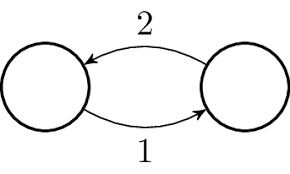
\includegraphics[width=0.2\textwidth]{figs/chap01/1.png}
\end{figure}
\item[-]
در هر یک از مسائل بسته به ذات مسئله نوع خاصی از گراف به عنوان ورودی در نظر گرفته می‌شود. برای مثال ورودی مسئله کوتاه ترین مسیر در حالت کلی یک گراف جهت دار و وزن دار است.
\end{itemize}
\end{frame}


%------------------------------------------------------------------------
\begin{frame}{يادآوری}
	\begin{itemize}\itemr
\item[-]
الگوریتم‌های گراف برخلاف بیشتر الگوریتم‌هایدارای دو متغییر تاثیر گذار در اندازه ورودی‌اند: تعداد یال‌ها (|E|) و تعداد رئوس (|V|) .
\item[-]
بر اساس قرارداد کتاب CLRS می‌توان در نمادهای مجانبی از قرار دادن نماد اندازه در اطراف V و E صرف‌نظر ‌کرد.

\item[-]
الگوریتم‌های گراف به طور معمول در دو حالت بررسی می‌شوند:
\item[الف]
زمانی که گراف متراکم باشد: در این حالت فرض میکنیم همه رئوس به هم متصل هستند بنابراین تعداد یال ها از مرتبه
\ath{V^2}
است.
\item[ب]
زمانی که گراف خلوت باشد:‌ در این حالت به طور معمول فرض می‌شود که تعداد یال‌ها از مرتبه
\ath{V}
است.

	\end{itemize}
\end{frame}

%------------------------------------------------------------------------
\begin{frame}{يادآوری}
\begin{itemize}\itemr
\item[-]
پیچیدگی زمانی ارائه شده برای یک الگوریتم گراف را می‌توان در دو حالت بالا تحلیل کرد. برای مثال تمرین زیر از کتاب CLRS را در نظر بگیرید:

\begin{figure}[h!]
\centering
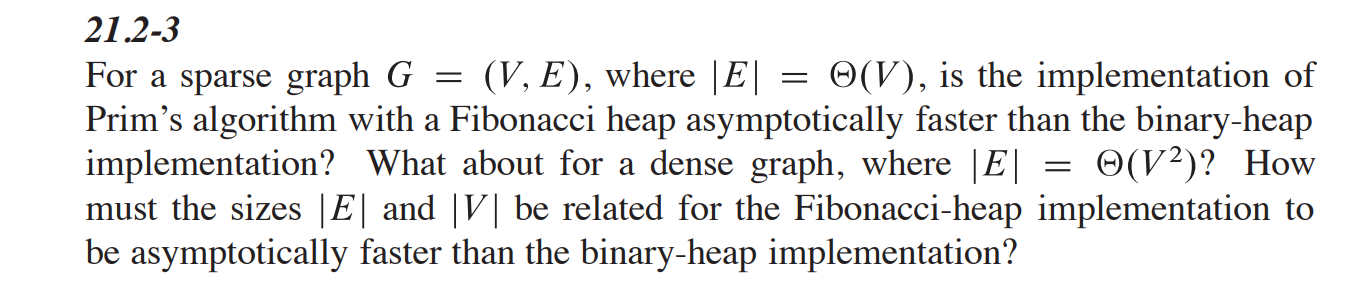
\includegraphics[width=\textwidth]{figs/chap01/2.png}
\end{figure}

\end{itemize}
\end{frame}

%------------------------------------------------------------------------
\begin{frame}{يادآوری}
\begin{itemize}\itemr
\item[-]
پیچیدگی زمانی الگوریتم پریم با استفاده از هرم دودویی از مرتبه
\m{O(E logV+V lgV)}
و با استفاده از هرم فیبوناچی از مرتبه
\m{O(E+V logV)}
است. با جایگذاری V به جای E در این دو تابع درمی‌یابیم که در گراف خلوت هر دو پیاده‌سازی‌ از لحاظ مجانبی سرعت یکسانی دارند و از مرتبه
\m{O(Vlg V)}
اند. اما در گراف متراکم پیاده‌سازی با هرم فیبوناچی از لحاظ مجانبی سریع تر و از مرتبه
\m{O(lgV^2)}
 است.
\item[-]
چنین تحلیلی در دیگر الگوریتم‌‌های گراف هم کاربرد دارد. برای مثال الگوریتم فلوید-وارشال از مرتبه زمانی
\m{O(V^3)}
 است. از تحلیل این تابع می‌توان نتیجه گرفت خلوت یا متراکم بودن گراف از نظر مجانبی تاثیری بر سرعت این الگوریتم ندارد.
\end{itemize}
\end{frame}




%------------------------------------------------------------------------
\begin{frame}{الگوریتم جانسون}
\begin{itemize}\itemr
\item[-]
الگوریتم جانسون
\fn{1}{Johnson Algorithm}
مانند الگوریتم فلوید وارشال برای یافتن کوتاه ترین مسیر بین هر دو راس گراف است. این الگوریتم برای گراف‌های خلوت پبچیدگی زمانی کمتری نسبت به بقیه روش‌ها (فلوید وارشال و روش شبیه‌سازی ضرب ماترسی) دارد.

\item[-]
الگوریتم جانسون -مانند الگوریتم بلمن فورد- می‌تواند روی گراف دارای یال منفی کوتاه ترین مسیر را به درستی محاسبه کند و وجود دور منفی در گراف را تشخیص و گزارش دهد. (گراف دارای دور منفی در مسئله کوتاه ترین مسیر یک حالت خطا محسوب می‌شود.)
\footnote{برای گراف دارای دور منفی یافتن کوتاه ترین مسیر ساده می‌تواند کاربرد داشته‌باشد. این مسئله ان‌پی-سخت است.}
\end{itemize}
\end{frame}

%------------------------------------------------------------------------
\begin{frame}{الگوریتم جانسون}
	\begin{itemize}\itemr
\item[-]
برای طراحی یک الگوریتم مسئله کوتاه‌ترین مسیر بین هر جفت رأس می‌توان V بار اجرا کردن یکی از الگوریتم‌های کوتاه‌ترین مسیرهای هم مبداء را به عنوان یک حد بالا برای مرتبه زمانی تحلیل کرد.

\item[-]
برای مثال
\m{|V|}
بار اجرای الگوریتم بلمن فورد مرتبه
\m{O(V^2E)}
و
\m{|V|}
بار اجرای الگوریتم دایجسترا مرتبه
\m{O(VE+V^2lgV)}
را به دست می‌دهد.
\item[-]
روش دوم سریع‌تر است امّا در گراف‌‌هایی که یال منفی داشته باشند به درستی کار نمی‌کند.
	\end{itemize}
\end{frame}

%------------------------------------------------------------------------
\begin{frame}{الگوریتم جانسون}
\begin{itemize}\itemr
\item[-]
الگوریتم جانسون نیز از ایده‌ایی مشابه استفاده می‌کند. این الگوریتم هر دو الگوریتم بلمن-فورد و دایجسترا را فراخوانی می‌کند؛
\item[۱]
جانسون در مرحله اول، الگوریتم بلمن-فورد را استفاده می‌کند تا وجود دور منفی را تشخیص دهد و در صورتی که دور منفی وجود داشت آن را گزارش داده و کار تمام می‌شود.
\item[۲]
در صورتی که دور منفی وجود نداشت، این الگوریتم با استفاده از روشی که در ادامه بررسی خواهد شد، همه وزن‌ها را به مقادیر غیر منفی نگاشت می‌کند.
\item[۳]
حال که همه وزن‌‌های غیر منفی شده‌اند برای هر رأس یک بار الگوریتم دایجسترا اجرا می‌شود تا کوتاه ترین مسیرها از هر رأس به بقیه رئوس محاسبه شوند.
\end{itemize}
\end{frame}

%------------------------------------------------------------------------
\begin{frame}{الگوریتم جانسون}
	\begin{itemize}\itemr
\item[-]
اما چطور باید وزن‌های گراف را به مقادیر غیر منفی نگاشت کرد؟ واضح است که بعد از تغییر وزن‌ها نباید کوتاه ترین مسیرها را تغییر کنند. برای مثال اضافه کردن یک مقدار ثابت به همه وزن‌ها نگاشت مناسبی نیست. برای درک بهتر این موضوع به مثال زیر توجه کنید:
\begin{center}
	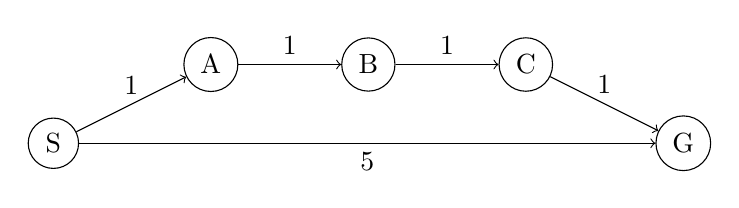
\begin{tikzpicture}[->]
		\node[circle,draw] (S) at (0,0) {S};
		\node[circle,draw] (G) at (8,0) {G};
		\node[circle,draw] (A) at (2,1) {A};
		\node[circle,draw] (B) at (4,1) {B};
		\node[circle,draw] (C) at (6,1) {C};

		\draw (S) -- node[below] {5} (G);
		\draw (S) -- node[above] {1} (A);
		\draw (A) -- node[above] {1} (B);
		\draw (B) -- node[above] {1} (C);
		\draw (C) -- node[above] {1} (G);
	\end{tikzpicture}
\end{center}
\item[-]
اضافه کردن یک واحد به همه یال‌ها کوتاه ترین مسیر از S به G را تغییر می‌دهد:

\begin{center}
	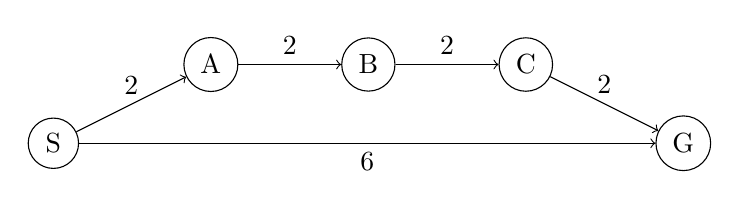
\begin{tikzpicture}[->]
		\node[circle,draw] (S) at (0,0) {S};
		\node[circle,draw] (G) at (8,0) {G};
		\node[circle,draw] (A) at (2,1) {A};
		\node[circle,draw] (B) at (4,1) {B};
		\node[circle,draw] (C) at (6,1) {C};

		\draw (S) -- node[below] {6} (G);
		\draw (S) -- node[above] {2} (A);
		\draw (A) -- node[above] {2} (B);
		\draw (B) -- node[above] {2} (C);
		\draw (C) -- node[above] {2} (G);
	\end{tikzpicture}
\end{center}

	\end{itemize}
\end{frame}

%------------------------------------------------------------------------
\begin{frame}{الگوریتم جانسون}
	\begin{itemize}\itemr
\item[-]
بیایید ویژگی‌های این تغییر وزن را به طور دقیق‌تر بررسی کنیم؛\\
فرض کنید وزن‌های گراف توسط تابعی به نام «تابع وزن»
\fn{1}{weight function}
داده شده. به طوری که وزن یال بین u و v برابر است با
\m{w(u, v)}.
آنگاه تابع وزن جدیدی مانند
\m{\hat{w}}
باید این دو ویژگی را داشته باشد:
\item[1]
به ازای هر
\m{u, v \in E}
مسیری مانند p با استفاده از تابع وزن
\m{w}
یک کوتاه ترین مسیر از u به v است اگر و تنها اگر مسیر p با استفاده از تابع وزن
\m{\hat{w}}
نیز یک کوتاه ترین مسیر باشد.
\item[2]
به ازای هر
\m{u, v \in E}
مقدار
\m{\hat{w}(u, v)}
غیر منفی باشد.
	\end{itemize}
\end{frame}

%------------------------------------------------------------------------
\begin{frame}{الگوریتم جانسون}
	\begin{itemize}\itemr
\item[-]
الگوریتم جانسون از این تغییر وزن استفاده می‌کند:
\begin{align*}
	\m{\hat{w}(u, v)} = \m{w(u, v)} + h(u) - h(v)
\end{align*}
\item[-]
به طوری که u رأس شروع و v رأس پایان یال است و h تابعی است که به هر رأس یک عدد حقیقی نسبت می‌دهد.
\item[-]
در ادامه ثابت خواهیم کرد که این تغییر وزن به ازای هر تابع h کوتاه‌ترین مسیرها را تغییر نمی‌دهد اما برای تبدیل همه وزن‌ها به مقادیر غیر منفی، تابع h باید به درستی تعریف شود.
	\end{itemize}
\end{frame}
%------------------------------------------------------------------------
\begin{frame}{الگوریتم جانسون}
	\begin{itemize}\itemr
		\item[-]
ابتدا باید ثابت ‌کنیم رابطه تغییر وزن ارائه شده ویژگی اول را ارضاء می‌کند.
		\item
فرض کنید
		\m{ p= \langle v_0, v_1, ..., v_k \rangle}
یک مسیر از
		\m{v_0}
به
		\m{v_k}
باشد. همچنین وزن کل مسیر p با تابع وزن w را با  w(p) نشان می‌دهیم. آنگاه
		\m{\hat{w}}
برابر است با:
		\begin{align*}
			\m{\hat{w}(p)= (\hat{w}(v_0, v_1) + h(v_0) -  h(v_1)) + (\hat{w}(v_1, v_2) + h(v_1) -  h(v_2)) + }
			\\
			\m{(\hat{w}(v_2, v_3) + h(v_2) -  h(v_3)) + ... + (\hat{w}(v_{k-1}, v_k) + h(v_{k-1}) -  h(v_k))}
		\end{align*}

	\end{itemize}
\end{frame}
%------------------------------------------------------------------------
\begin{frame}{الگوریتم جانسون}
	\begin{itemize}\itemr
\item
رابطه بالا نشان می‌دهد برای هر رأس مثل u، مقدار h(u) به وزن یک یال اضافه می‌شود و از یال بعدی کسر می‌شود (به غیر از رأس ابتدا و انتهای مسیر). بعد از ساده‌سازی به این رابطه می‌رسیم:
\begin{align*}
	\m{\hat{w}(p)=w(p) + h(h(v_0) - h(v_k)}
\end{align*}
\item
بنابراین برای هر دو رأس مشخص به همه کوتاه‌ترین مسیرهای بین آن دو رأس یک مقدار ثابت اضافه می‌شود پس این نگاشت وزن کوتاه ترین مسیرها را تغییر نمی‌دهد.
	\end{itemize}
\end{frame}

%------------------------------------------------------------------------
\begin{frame}{الگوریتم جانسون}
	\begin{itemize}\itemr
		\item[-]
هدف بعدی این است که شرایطی فراهم کنیم که ویژگی دوم هم برقرار باشد. برای این کار یک رأس جدید به نام s به گراف اضافه می‌کنیم. سپس این رأس را با یال‌هایی با وزن صفر به همه رئوس دیگر متصل می‌کنیم به طوری که یال ‌ها از s خارج شوند.
		\begin{figure}[h!]
			\centering
			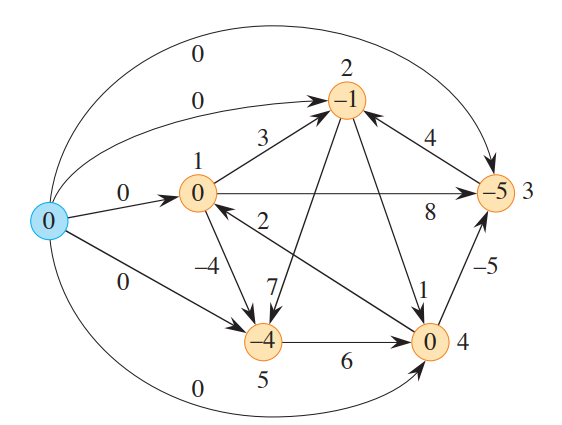
\includegraphics[width=.4\textwidth]{figs/chap02/4.png}
		\end{figure}
شکل بالا نمونه‌ایی از این تغییر را نشان می‌دهد (رأس آبی رنگ به گراف اضافه شده‌است).
	\end{itemize}
\end{frame}

%------------------------------------------------------------------------
\begin{frame}{الگوریتم جانسون}
	\begin{itemize}\itemr
		\item
سپس تعریف می‌کنیم مقدار h برای هر رأس مثل v برابر است با کوتاه ترین مسیر از s به v . در شکل بالا نیز اعداد نوشته‌شده بر رأس‌ها به همین طریق محاسبه شده‌اند.
		\item
حال با استفاده از نامساوی مثلثاتی می‌دانیم که به ازای هر
		\m{(u, v \in E)}
رابطه زیر برقرار است:
		\begin{center}
			\m{h(v) \leqslant h(u)+w(u, v) } \\

		\end{center}
		\item
اگر رابطه بالا برقرار نباشد نتیجه می‌شود که مسیر h(v) کوتاه‌ترین مسیر نبوده و به تناقض می‌رسیم.
		\item
سپس h(u) را به سمت راست نامساوی می‌بریم:
		\begin{center}
			\m{0\leqslant w(u, v) + h(u) - h(v)}
		\end{center}
		\item
سمت راست این نامساوی همان رابطه‌ایی است که برای $\hat{w}$ تعریف شد. بنابراین ثابت شد که به ازای هر
		\m{(u, v \in E)}
مقدار $\hat{w}$ غیر منفی است.
	\end{itemize}
\end{frame}

%------------------------------------------------------------------------
\begin{frame}{الگوریتم جانسون}
	\begin{itemize}\itemr
		\item[-]
درستی الگوریتم جانسون ثابت شد. شکل زیر یک نمونه از گراف تغییر وزن یافته توسط الگوریتم جانسون است:
		\begin{figure}[h!]
			\centering
			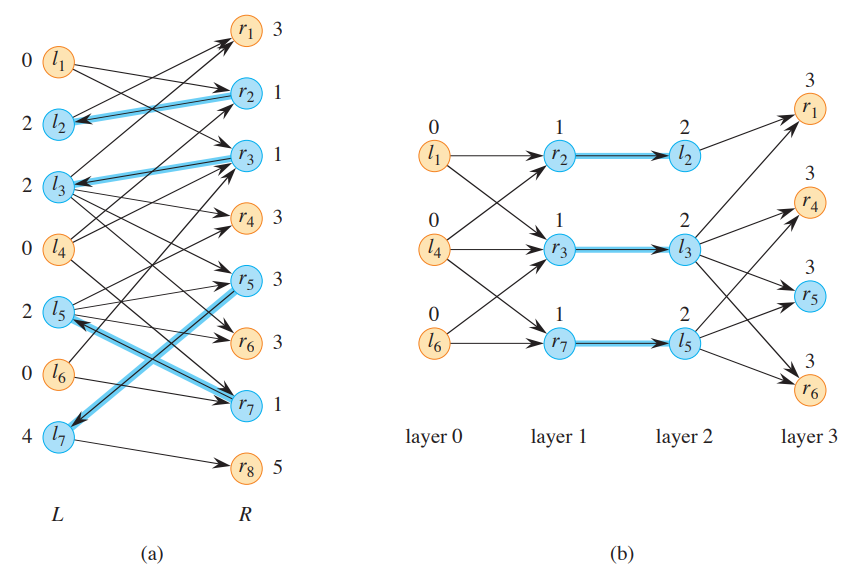
\includegraphics[width=.3\textwidth]{figs/chap02/5.png}
		\end{figure}

		\item[-]
قبلا اشاره شد که الگوریتم جانسون از الگوریتم بلمن-فورد برای تشخیص دور منفی استفاده می‌کند. همچنین دیدم که برای محاسبه تابع h نیاز به مقادیر کوتاه‌ترین مسیر از s به بقیه رئوس نیاز داریم. می‌دانیم الگوریتم بلمن-فورد توانایی محاسبه هر دوی این موارد را دارد. بنابراین الگوریتم جانسون با یک بار اجرای بلمن-فورد هم کوتاه‌ترین مسیرها از s را محاسبه می‌کند و هم وجود دور منفی را تشخیص می‌دهد.

	\end{itemize}
\end{frame}

%------------------------------------------------------------------------
\begin{frame}{الگوریتم جانسون}
	\begin{itemize}\itemr
		\item[-]
		برای یافتن وزن اصلی یک مسیر از رابطه زیر استفاده می‌کنیم:
		\begin{center}
			\m{w(p(u, v)) = \hat{w}(p(u, v)) + h(v) - h(u) }
		\end{center}

		\item[-]
		در نهایت به تحیلی پیچیدگی زمانی الگوریتم جانسون می‌پردازیم:
		\item
		اجرای $|V|$ بار الگوریتم دایجسترا زمان‌برترین مرحله الگوریتم جانسون است بنابراین -مانند دایجسترا- باید گراف را در لیست مجاورتی ذخیره کنیم. حال اگر فرض کنیم الگوریتم دایجسترا با استفاده از هرم فیبوناچی پیاده‌سازی شده‌است، پیچیدگی زمانی برابر است با
		\m{O(V^2lgV+VE)}
		که از ضرب یک
		\m{|V|}
		در مرتبه زمانی دایجسترا به دست آمده‌است.
		\item
		در صورتی که گراف خلوت باشد مرتبه زمانی این الگوریتم برابر است
		\m{O(V^2lgV)}.
		در حالی که الگوریتم فلوید-وارشال برای گراف خلوت از مربته زمانی
		\m{O(V^3)}
		است.

	\end{itemize}
\end{frame}


%%%%%%%%%%%%%%%%%%%%%%%%%
\section{الگوریتم‌های تقسیم و حل}
%%%%%%%%%%%%%%%%%%%%%%%%%


\begin{frame}{‌طراحی الگوریتم با استقرا}
\begin{itemize}\itemr
\item[-]
استقرای ریاضی
\fn{1}{induction}
روشی است برای اثبات درستی گزاره
\m{P(n)}
برای همه اعداد طبیعی
\m{n}
. به عبارت دیگر هنگامی که می‌خواهیم درستی گزاره‌های
\m{P(1)}
،
\m{P(2)}
،
\m{\cdots}
،
\m{P(n)}
را ثابت کنیم، می‌توانیم از استقرا استفاده کنیم.
\item[-]
به زبان استعاری با استفاده از استقرا ثابت می‌کنیم که می‌توانیم هر نردبانی را با طول دلخواه یا بینهایت بالا برویم اگر ثابت کنیم که می‌‌توانیم برروی پله اول برویم (پایهٔ استقرا
\fn{2}{base case}
) و همچنین ثابت کنیم اگر برروی پلهٔ
\m{n}
بودیم می‌توانیم برروی پله
\m{n+1}
نیز گام بگذاریم (گام استقرا
\fn{3}{induction step}
).
\item[-]
بنابراین در روش استقرایی برای اثبات درستی
\m{P(n)}
باید ثابت کنیم
\m{P(1)}
درست است (پایهٔ استقرا) و همچنین اگر
\m{P(n)}
درست باشد، آنگاه
\m{P(n+1)}
نیر درست است (گام استقرا).
\end{itemize}
\end{frame}


\begin{frame}{‌طراحی الگوریتم با استقرا}
\begin{itemize}\itemr
\item[-]
استقرای ریاضی براساس اصل دومینو
\fn{1}{domino principle}
است. فرض کنید تعداد زیادی دومینو به صورت ایستاده در کنار یکدیگر قرار گرفته‌اند و می‌خواهیم همهٔ دومینوهای ایستاده را بیاندازیم. برای اینکه همهٔ دومینوها بر زمین بیفتند کافی است دومینوها به گونه‌ای قرار داده شوند که با افتادن اولین دومینو، دومین دومینو برزمین بیافتد و با افتادن دومی، سومی و به همین ترتیب با افتادن
\m{n}
امین دومینو،
\m{n+1}
امین دومینو بر زمین بیافتد. سپس کافی است به اولین دومینو ضربه‌ای بزنیم تا همه دومینوهای ایستاده بیافتند و نیازی به انداختن تک‌تک آنها نداریم.
\end{itemize}
\end{frame}

\iffalse
\begin{frame}{‌طراحی الگوریتم با استقرا}
\begin{itemize}\itemr
\item[-]
در طراحی یک مسئله به روش استقرایی، باید برای پاسخ مسئله یک رابطه پیدا کنیم و پاسخ مسئله را به روش استقرایی اثبات کنیم. و سپس می‌توانیم از رابطهٔ به دست آمده برای حل مسئله استفاده کنیم.
\item[-]
برای مثال فرض کنید می‌خواهیم جمع
\m{n}
عدد اول صحیح را به دست آوریم. برای این کار
\m{n}
عدد را با یکدیگر جمع کنیم. پس الگوریتم در واقع
\m{O(n)}
است.
\item[-]
برای حل این مسئله به روش استقرایی باید رابطه‌ای برای جواب مسئله پیدا کنیم. به عبارت دیگر آیا عبارتی وجود دارد که توسط آن بتوان جمع
\m{n}
عدد اول اعداد صحیح را به دست آورد؟
\end{itemize}
\end{frame}
\fi

\begin{frame}{‌طراحی الگوریتم با استقرا}
\begin{itemize}\itemr
\item[-]
برای مثال با استفاده از استقرا می‌توان اثبات کرد:
\begin{align*}
\m{P(n) = 1 + 2 + 3 + \cdots + n = \frac{n(n+1)}{2}}
\end{align*}
\item[-]
باید اثبات کنیم
\m{P(1) = \frac{1(2)}{2}}
درست است (پایهٔ استقرا) و همچنین اگر
\m{P(n) = \frac{n(n+1)}{2}}
باشد آنگاه
\m{P(n+1) = \frac{(n+1)(n+2)}{2}}
نیز درست است (گام استقرا).
\end{itemize}
\end{frame}


\begin{frame}{‌طراحی الگوریتم با استقرا}
\begin{itemize}\itemr
\item[-]
اثبات : 
\item[-]
پایه استقرا درست است زیرا 
\m{P(1) = 1 = \frac{1(2)}{2} = 1}
\item[-]
می‌دانیم
\m{P(n+1) = P(n) + (n+1)}
بنابراین
\m{P(n+1) = \frac{n(n+1)}{2} + (n+1)} .
با بسط این رابطه به دست می‌آوریم
\m{P(n+1) = \frac{(n+1)(n+2)}{2}} .
بنابراین گام استقرا نیز درست است.
\item[-]
با استفاده از این رابطه برای محاسبهٔ
\m{n}
عدد کافی است از رابطه
\m{P(n)}
استفاده کنیم. این الگوریتم در زمان
\m{O(1)}
انجام می‌شود، در حالی که جمع 
\m{n}
عدد با استفاده از یک حلقه در زمان
\m{O(n)}
انجام می‌شود.
\end{itemize}
\end{frame}



\begin{frame}{‌طراحی الگوریتم با استقرا}
\begin{itemize}\itemr
\item[-]
استقرای ریاضی در طراحی الگوریتم‌ها بسیار پر استفاده است.
\item[-]
برای طراحی یک الگوریتم برای حل یک مسئله با استفاده از استقرا کافی است :
\item[۱.]
مسئله را در حالت پایه یعنی حالتی که اندازه ورودی کوچک است حل کنیم.
\item[۲.]
نشان‌دهیم چگونه می‌توان یک مسئله را با استفاده از یک زیر مسئله (یعنی مسئله‌ای با اندازهٔ کوچک‌تر) حل کرد.
\end{itemize}
\end{frame}


\begin{frame}{‌طراحی الگوریتم با استقرا}
\begin{itemize}\itemr
\item[-]
فرض کنید می‌خواهیم به ازای دنباله‌ای از اعداد حقیقی
\m{a_0}
،
\m{a_1}
،
\m{a_2}
،
\m{\cdots}
،
\m{a_n}
و عدد داده شده
\m{x}،
مقدار چند جمله‌ای زیر را محاسبه کنیم.\\
\begin{align*}
\m{P_n(x) = a_nx^n + a_{n-1}x^{n-1} + \cdots + a_1x + a_0}
\end{align*}
\end{itemize}
\end{frame}


\begin{frame}{‌طراحی الگوریتم با استقرا}
\begin{itemize}\itemr
\item[-]
یک الگوریتم بدیهی برای حل این مسئله با جایگذاری اعداد
\m{a_i}
و
\m{x}
در چند جمله
\m{P_n(x)}
مقدار آن را محاسبه می‌کند.
\begin{algorithm}[H]\alglr
\caption{Compute Polynomial}
  \begin{algorithmic}[1]
   \Func{ComputePolynomial}{a[], x}
    \State P = a[0]
    \For{i = 1 to n}
      \State X = 1
      \For{j = 1 to i}
          \State X = X * x
       \EndFor
       \State P = P + a[i] * X
     \EndFor
     \State \Return P                          
  \end{algorithmic}
  \label{alg:merge}
\end{algorithm}
\item[-]
پیچیدگی زمانی این الگوریتم
\m{O(n^2)}
است.
\item[-]
حال می‌خواهیم با استفاده از استقرا این مسئله را در زمان کمتری حل کنیم.
\end{itemize}
\end{frame}


\begin{frame}{‌طراحی الگوریتم با استقرا}
\begin{itemize}\itemr
\item[-]
برای حل مسئله با استفاده از استقرا باید بتوانیم مسئله را بر اساس یک زیر مسئله بیان کنیم.
\item[-]
یک زیر مسئله از مسئلهٔ محاسبه چند جمله‌ای را به صورت زیر در نظر بگیرید.
\begin{align*}
\m{P_{n-1}(x) = a_nx^{n-1} + a_{n-1}x^{n-2} + \cdots + a_1}
\end{align*}
\item[-]
فرض کنید جواب
\m{P_{n-1}(x)}
داده شده است. چگونه می‌توانیم
\m{P_n(x)}
را محاسبه کنیم؟
\end{itemize}
\end{frame}


\begin{frame}{‌طراحی الگوریتم با استقرا}
\begin{itemize}\itemr
\item[-]
برای محاسبه
\m{P_n(x)}
می‌توانیم رابطه‌ای به صورت زیر بنویسیم.
\begin{align*}
\m{P_n(x) = x \cdot P_{n-1}(x) + a_0}
\end{align*}
\item[-]
همچنین می‌توانیم
\m{P_{n-1}(x)}
را بر اساس
\m{P_{n-2}(x)}
محاسبه کنیم.
\item[-]
داریم :
\begin{align*}
\m{P_{n-2}(x) = a_nx^{n-2} + a_{n-1}x^{n-3} + \cdots + a_2}
\end{align*}
\item[-]
بنابراین خواهیم داشت :
\begin{align*}
\m{P_{n-1}(x) = x \cdot P_{n-2}(x) + a_1}
\end{align*}
\end{itemize}
\end{frame}


\begin{frame}{‌طراحی الگوریتم با استقرا}
\begin{itemize}\itemr
\item[-]
در حالت کلی برای محاسبه
\m{P_{n-j}(x)}
با استفاده از یک زیرمسئله می‌توانیم رابطهٔ زیر را ارائه کنیم:
\begin{align*}
\m{P_{n-j}(x) = x \cdot P_{n-(j+1)}(x) + a_j}
\end{align*}
\item[-]
در حالت پایه داریم:
\begin{align*}
\m{P_0(x) = a_n}
\end{align*}
\end{itemize}
\end{frame}


\begin{frame}{‌طراحی الگوریتم با استقرا}
\begin{itemize}\itemr
\item[-]
فرض کنیم
\m{n - j = i}
، در اینصورت خواهیم داشت :
\begin{align*}
\left\{ \begin{array}{lcl}
\m{P_i(x) = x \cdot P_{i-1}(x) + a_{n-i}} & \m{i > 0} & \text{اگر} \\
\m{P_0(x) = a_n} & \m{i = 0} & \text{اگر}
\end{array}\right.
\end{align*}
\end{itemize}
\end{frame}


\begin{frame}{‌طراحی الگوریتم با استقرا}
\begin{itemize}\itemr
\item[-]
بنابراین با استفاده از رابطه بازگشتی به دست آمده می‌توانیم الگوریتمی به صورت زیر بنویسیم.
\begin{algorithm}[H]\alglr
\caption{Compute Polynomial}
  \begin{algorithmic}[1]
   \Func{ComputePolynomial}{a[], x}
    \State P = a[n]
    \For{i = 1 to n}
       \State P = x * P + a[n-i]
     \EndFor  
     \State \Return P                           
  \end{algorithmic}
  \label{alg:merge}
\end{algorithm}
\item[-]
پیچیدگی زمانی این الگوریتم
\m{O(n)}
است که از الگوریتم بدیهی که در زمان
\m{O(n^2)}
چند جمله‌ای را محاسبه می‌کند سریع‌تر است.
\end{itemize}
\end{frame}


\begin{frame}{‌طراحی الگوریتم با استقرا}
\begin{itemize}\itemr
\item[-]
این الگوریتم به روش هورنر
\fn{1}{Horner's method}
معروف است که توسط ریاضی‌دان انگلیسی ویلیام هورنر
\fn{2}{William Horner}
ابداع شده است، گرچه خود هورنر آن را به ریاضی‌دان فرانسوی-ایتالیایی ژوزف لاگرانژ
\fn{3}{Joseph-Louis Lagrange}
نسبت داده است. گفته می‌شود این الگوریتم قبل از لاگرانژ احتمالاً توسط ریاضی‌دانان ایرانی و چینی ابداع شده است.
\begin{align*}
&\m{a_0 + a_1x + a_2x^2 + \cdots + a_nx^n =} \\
&~~~~~~~~~~~~~~~~~~~~~~~~~~~~~~~\m{a_0 + x ( a_1 + x (a_2 + x ( a_3 + \cdots + x (a_{n-1} + xa_n) \cdots)))}
\end{align*}
\end{itemize}
\end{frame}
\begin{frame}{‌الگوریتم‌های تقسیم و حل}
\begin{itemize}\itemr
\item[-]
برای حل یک مسئله به روش‌های متنوعی می‌توان الگوریتم طراحی کرد.
\item[-]
الگوریتم مرتب‌سازی درجی یک الگوریتم ساده است که به روش افزایشی با مرتب‌سازی زیر آرایه‌های کوچک‌تر آرایه آغاز می‌شود و در نهایت کل آرایه را مرتب می‌کند. در واقع به ازای هر عنصر
\code{A[i]}
، این عنصر در مکان مناسب خود در زیر آرایه مرتب شدهٔ
\code{A[1 : i-1]}
قرار می‌گیرد.
\end{itemize}
\end{frame}


\begin{frame}{‌الگوریتم‌های تقسیم و حل}
\begin{itemize}\itemr
\item[-]
در این قسمت با روشی دیگر برای حل مسئله‌های محاسباتی آشنا می‌شویم، که به آن روش تقسیم و حل
\fn{1}{divide and conquer method}
(تقسیم و غلبه)
گفته می‌شود و الگوریتم‌هایی که از این روش استفاده می‌کنند، در دستهٔ الگوریتم‌های تقسیم و حل قرار می‌گیرند.
\item[-]
از روش تقسیم و حل برای حل مسئلهٔ مرتب‌سازی استفاده می‌کنیم و زمان اجرای آن را محاسبه می‌کنیم.
\item[-]
خواهیم دید که با استفاده از این روش، مسئلهٔ مرتب‌سازی در زمان کمتری نسبت به الگوریتم مرتب‌سازی درجی حل می‌شود.
\end{itemize}
\end{frame}


\begin{frame}{‌الگوریتم‌های تقسیم و حل}
\begin{itemize}\itemr
\item[-]
بسیاری از  الگوریتم‌های کامپیوتری بازگشتی
\fn{1}{recursive}
هستند. در یک الگوریتم بازگشتی، برای حل یک مسئله با یک ورودی معین ، خود الگوریتم با ورودی‌های کوچکتر فراخوانی می‌شود.
\item[-]
برای مثال، برای به دست آوردن فاکتوریل عدد n کافی است فاکتوریل عدد n-1 را فراخوانی کنیم.
\item[-]
به الگوریتم‌هایی که ورودی مسئله را تقسیم می‌کنند و به طور بازگشتی الگوریتم را برای قسمت‌های تقسیم شده فراخوانی می‌‌کنند، الگوریتم‌های تقسیم و حل گفته می‌شود.
\end{itemize}
\end{frame}


\begin{frame}{‌الگوریتم‌های تقسیم و حل}
\begin{itemize}\itemr
\item[-]
به عبارت دیگر یک الگوریتم تقسیم و حل یک مسئله را به چند زیر مسئله تقسیم می‌کند که مشابه مسئلهٔ اصلی هستند و الگوریتم را برای زیر مسئله‌ها فراخوانی می‌کند و سپس نتایج به دست آمده از زیر مسئله‌ها را با هم ترکیب می‌کند تا نتیجهٔ نهایی برای مسئلهٔ اصلی به دست آید.
\item[-]
معمولاً‌ پس از شکسته شدن یک مسئله به زیر مسئله‌ها، زیر مسئله‌هایی به دست می‌آیند که می‌توانند دوباره شکسته شوند و این روند تا جایی ادامه پیدا می‌کند که مسئله امکان شکسته شدن نداشته باشد. وقتی مسئله امکان شکسته شدن نداشته باشد، حالت پایه
\fn{1}{base case}
به دست می‌آید که حل مسئله در حالت پایه به سادگی امکان پذیر است.
\end{itemize}
\end{frame}


\begin{frame}{‌الگوریتم‌های تقسیم و حل}
\begin{itemize}\itemr
\item[-]
یک الگوریتم تقسیم و حل از سه مرحلهٔ زیر تشکیل شده‌است.\\
1. تقسیم
\fn{1}{divide}
: مسئله به چند زیر مسئله که نمونه‌های کوچکتر مسئلهٔ اصلی هستند تقسیم می‌شود.\\
۲. حل یا غلبه
\fn{2}{conquer}
: زیر مسئله‌ها به صورت بازگشتی حل می‌شوند.\\
۳. ترکیب
\fn{3}{combine}
: زیر مسئله‌های حل شده با یکدیگر ترکیب می‌شوند تا جواب مسئلهٔ اصلی به دست بیاید.
\end{itemize}
\end{frame}


\begin{frame}{‌مرتب‌سازی ادغامی}
\begin{itemize}\itemr
\item[-]
الگوریتم مرتب‌سازی ادغامی
\fn{1}{merge sort}
در دستهٔ الگوریتم‌های تقسیم و حل قرار می‌گیرد. با شروع از آرایهٔ
\code{A[1:n]}
، در هر مرحله یکی از زیر آرایه‌های
\code{A[p:r]}
مرتب می‌شود و سپس این زیر آرایه‌ها با یکدیگر ادغام می‌شوند تا آرایهٔ اصلی مرتب شود. برای هر یک از زیر آرایه‌ها، الگوریتم مرتب‌سازی ادغامی فراخوانی می‌شود و به همین نحو، آن زیر آرایه‌ها تقسیم شده و به روش بازگشتی مرتب می‌شوند.
\end{itemize}
\end{frame}


\begin{frame}{‌مرتب‌سازی ادغامی}
\begin{itemize}\itemr
\item[-]
مراحل انجام مرتب‌سازی ادغامی به صورت زیر است :
\item[۱.]
تقسیم : آرایهٔ
\code{A[p:r]}
به دو زیرآرایهٔ مساوی تقسیم می‌شود. اگر 
\code{q} 
وسط 
\code{p}
 و 
\code{r}
  باشد، آنگاه دو آرایهٔ به دست آمده عبارتند از
\code{A[p:q]}
و
\code{A[q+1:r]}
. در مرحلهٔ اول 
\code{p}
 برابر با 
\code{1}
  و 
\code{r}
   برابر است با 
\code{n} .
\item[۲.]
حل : الگوریتم به صورت بازگشتی برای دو زیر آرایهٔ
\code{A[p:q]}
و
\code{A[q+1:r]}
فراخوانی می‌شود.
\item[۳.]
ترکیب : با ادغام دو آرایهٔ
\code{A[p:q]}
و
\code{A[q+1:r]}
که هر دو مرتب شده هستند، آرایهٔ مرتب شدهٔ
\code{A[p:r]}
به دست می‌آید.
\end{itemize}
\end{frame}


\begin{frame}{‌مرتب‌سازی ادغامی}
\begin{itemize}\itemr
\item[-]
این الگوریتم به طور بازگشتی فراخوانی می‌شود تا به حالت پایه برسیم.
در حالت پایه، آرایهٔ به دست آمده شامل تنها یک عنصر است که در این حالت آرایه نیاز به مرتب‌سازی ندارد. در واقع هنگامی به حالت پایه می‌رسیم که 
\code{p}
 برابر با 
\code{r}
  باشد.
\item[-]
در مرحلهٔ ادغام، با فرض اینکه دو آرایهٔ به دست آمده مرتب شده هستند، دو آرایه باید به نحوی با یکدیگر ترکیب شوند که آرایهٔ به دست آمده مرتب شده باشد.
\end{itemize}
\end{frame}


\begin{frame}{‌مرتب‌سازی ادغامی}
\begin{itemize}\itemr
\item[-]
الگوریتم مرتب‌سازی ادغامی به صورت زیر است.
\begin{algorithm}[H]\alglr
  \caption{Merge Sort} 
  \begin{algorithmic}[1]
    \Func{Merge-Sort}{A, p, r}
    \If{p >= r}	\LeftComment{zero or one element?}
    	\State \Return
    \EndIf    
    \State q = $\lfloor$ (p+r)/2 $\rfloor$	\LeftComment{ midpoint of A[p:r]}
    \State Merge-Sort (A, p, q)	\LeftComment{ recursively sort A[p:q]}
    \State Merge-Sort (A, q+1, r)	\LeftComment{ recursively sort A[q+1:r]}
    \State Merge (A, p, q, r) \LeftComment{Merge A[p:q] and A[q+1:r] into A[p:r].}
  \end{algorithmic}
  \label{alg:merge-sort}
\end{algorithm}
\end{itemize}
\end{frame}

\begin{frame}{‌مرتب‌سازی ادغامی}
\begin{itemize}\itemr
\item[-]
برای ادغام دو زیرآرایه از الگوریتم زیر استفاده می‌کنیم.
\begin{algorithm}[H]\alglr
  \caption{Merge Sort} 
  \begin{algorithmic}[1]
    \Func{Merge}{A, p, q, r}
    \State nl = q - p + 1 \LeftComment{ length of A[p:q]}
    \State nr = r - q \LeftComment{ length of A[q+1 : r]}
    \State let L[ 0 : nl - 1 ] and R[ 0 : nr - 1 ] be new arrays
    \For{i = 0 \To nl - 1} \LeftComment{ copy A[p:q] into L[0:nl - 1]}
      \State L[i] = A[p+i]
    \EndFor
    \For{j = 0 to nr - 1} \LeftComment{copy A[q+1:r] into L[0:nr - 1]} 
      \State R[j] = A[q + j + 1]
     \EndFor
  \end{algorithmic}
  \label{alg:merge}
\end{algorithm}
\end{itemize}
\end{frame}


\begin{frame}{‌مرتب‌سازی ادغامی}
\begin{itemize}\itemr
\item[-]
\begin{algorithm}[H]\alglr
  \caption{Merge Sort} 
  \begin{algorithmic}[1]
  \setcounter{ALG@line}{7}
    \Func{Merge}{A, p, q, r}
      \State i = 0 \LeftComment{ i indexes the smallest remaining element in L}
      \State j = 0 \LeftComment{j indexes the smallest remaining element in R}
      \State k = p \LeftComment{ k indexes the location in A to fill}
    \newline\LeftComment{ As long as each of the arrays L and R contains un unmerged element, copy the smallest unmerged element back into A[p : r].}                              
    \While{ i < nl \Aand j < nr}
          \If {L[i] <= R[j]}
              \State A[k] = L[i]
              \State i = i + 1
          \Else 
              \State A[k] = R[j]
              \State j = j + 1
           \EndIf
          \State k = k + 1
      \EndWhile
  \end{algorithmic}
  \label{alg:merge}
\end{algorithm}
\end{itemize}
\end{frame}



\begin{frame}{‌مرتب‌سازی ادغامی}
\begin{itemize}\itemr
\item[-]
\begin{algorithm}[H]\alglr
  \caption{Merge Sort} 
  \begin{algorithmic}[1]
    \setcounter{ALG@line}{18}
    \Func{Merge}{A, p, q, r}
    \newline\LeftComment{ Having gone through one of L and R entirely, copy the  remainder of the other to the end of A[p:r]}                                    
    \While{i < nl}
             \State A[k] = L[i]
             \State i = i + 1
             \State k = k + 1
     \EndWhile      
    \While{ j < nr}
            \State A[k] = R[j]
            \State j = j + 1
            \State k = k + 1 
      \EndWhile                                             
  \end{algorithmic}
  \label{alg:merge}
\end{algorithm}
\end{itemize}
\end{frame}


\begin{frame}{‌مرتب‌سازی ادغامی}
\begin{itemize}\itemr
\item[-]
یک مثال از ادغام دو زیر آرایه در شکل زیر نشان داده شده‌است.
\begin{figure}
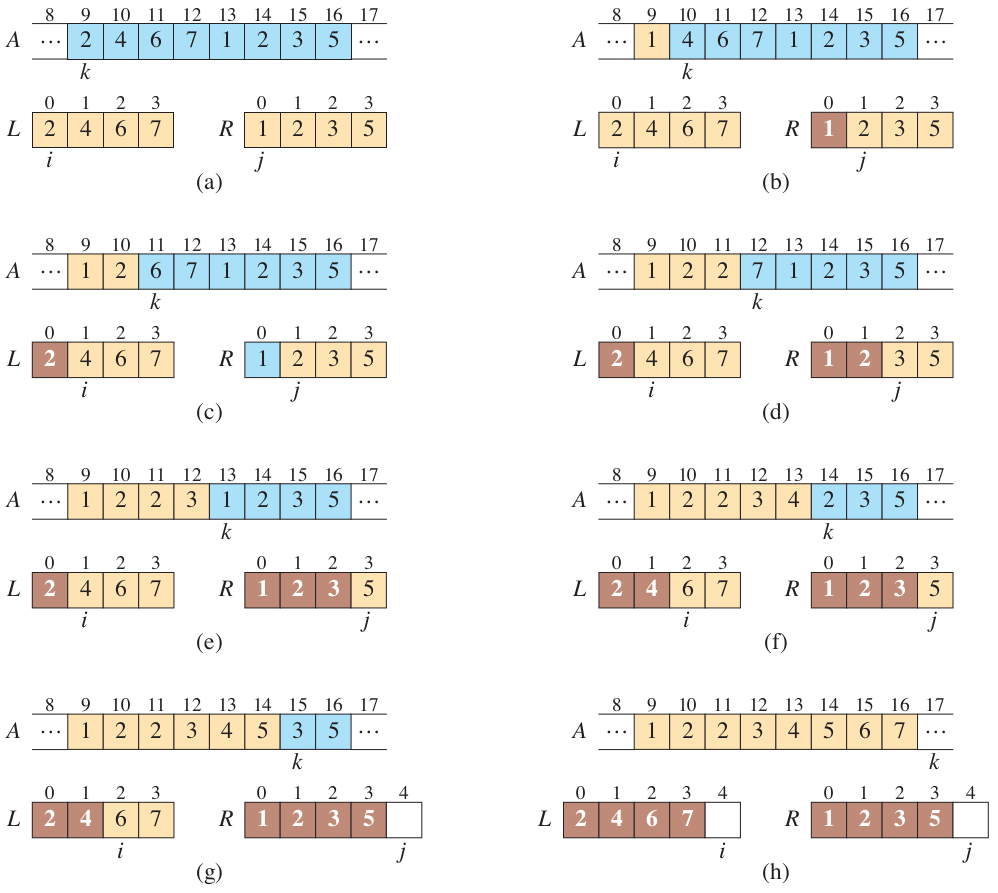
\includegraphics[width=0.5\textwidth]{figs/chap03/merge-example}
\end{figure}
\end{itemize}
\end{frame}


\begin{frame}{‌مرتب‌سازی ادغامی}
\begin{itemize}\itemr
\item[-]
در حلقهٔ تکرار الگوریتم ادغام، در هر تکرار یکی از عناصر در آرایهٔ A کپی می‌شوند و در کل تا پایان الگوریتم n عنصر در آرایه کپی می‌شوند، پس زمان اجرای این الگوریتم
\ath{n}
است.
\end{itemize}
\end{frame}


\begin{frame}{‌مرتب‌سازی ادغامی}
\begin{itemize}\itemr
\item[-]
یک مثال مرتب‌سازی ادغامی در شکل زیر نشان داده شده‌است.
\begin{figure}
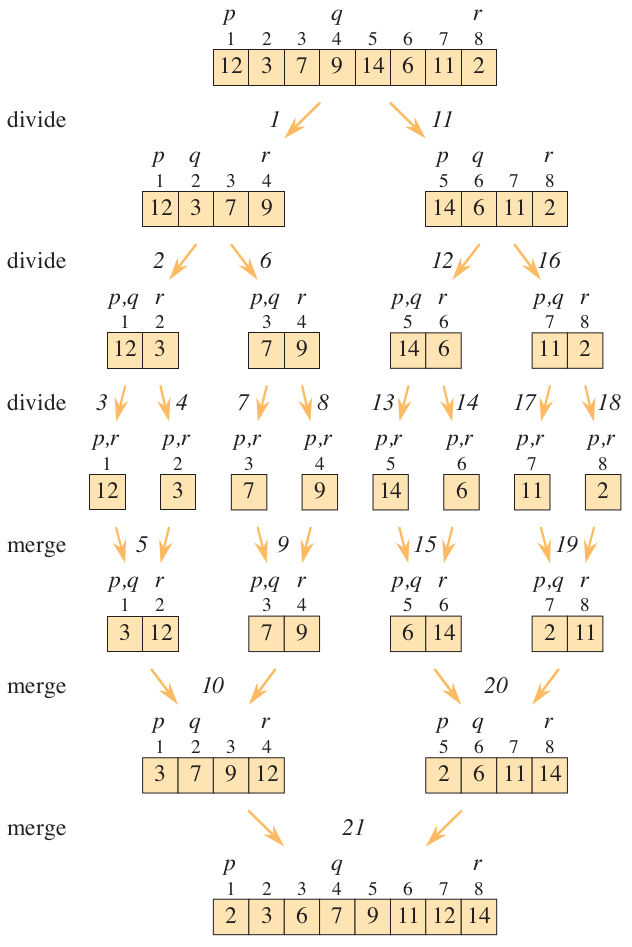
\includegraphics[width=0.3\textwidth]{figs/chap03/merge-sort-example}
\end{figure}
\end{itemize}
\end{frame}


\begin{frame}{‌مرتب‌سازی ادغامی}
\begin{itemize}\itemr
\item[-]
وقتی یک مسئله به صورت بازگشتی طراحی می‌شود، زمان اجرای آن را نیز معمولا با استفاده از معادلات بازگشتی
\fn{1}{recurrence equation}
به دست می‌آوریم.
در این معادلات بازگشتی، زمان اجرای یک الگوریتم با ورودی اندازهٔ n توسط زمان اجرای همان الگوریتم با ورودی‌هایی از اندازه‌های کوچک‌تر به دست می‌آید. روش‌های متعددی برای حل مسائل بازگشتی وجود دارند که می‌توان از آنها استفاده کرد.
\end{itemize}
\end{frame}


\begin{frame}{‌مرتب‌سازی ادغامی}
\begin{itemize}\itemr
\item[-]
به طور کلی اگر فرض کنیم زمان اجرای یک الگوریتم برای ورودی با اندازهٔ n برابر با
\m{T(n)}
باشد و توسط روش تقسیم و حل مسئلهٔ مورد نظر به
\m{a}
زیر مسئله تقسیم شود که اندازه ورودی هر کدام
\m{n/b}
باشد، آنگاه به زمان
\m{aT(n/b)}
برای حل مسئله نیاز داریم.
\item[-]
همچنین اگر به زمان 
\m{D(n)}
 برای تقسیم مسئله به زیر مسئله‌ها و به زمان
\m{C(n)} 
 برای ادغام زیر مسئله‌ها نیاز داشته باشیم، آنگاه این زمان‌ها به زمان مورد نیاز برای حل مسئله افزوده می‌شوند.
\end{itemize}
\end{frame}


\begin{frame}{‌مرتب‌سازی ادغامی}
\begin{itemize}\itemr
\item[-]
فرض کنید در حالت پایه، یعنی وقتی اندازهٔ ورودی از یک مقدار معین کوچکتر است، اجرای برنامه در زمان ثابت انجام شود، یعنی زمان اجرای برنامه در حالت پایه به اندازهٔ ورودی n بستگی نداشته باشد.
\item[-]
در حالت کلی زمان اجرای یک الگوریتم تقسیم و حل را می‌توانیم با استفاده از رابطهٔ بازگشتی زیر بنویسیم.
\begin{align*}
\m{T(n)} = \left\{\begin{array}{lr}
          \m{\Theta (1)}& \m{n < n_0}~\text{اگر}\\
          \m{D(n) + aT(n/b) + C(n)}&\text{در باقی حالات}
\end{array}\right.
\end{align*}
\end{itemize}
\end{frame}


\begin{frame}{‌مرتب‌سازی ادغامی}
\begin{itemize}\itemr
\item[-]
حال زمان اجرای الگوریتم مرتب‌سازی ادغامی را در بدترین حالت به ازای یک آرایهٔ با طول n تحلیل می‌کنیم.\\
۱. تقسیم : تقسیم کردن آرایه به دو قسمت در زمان ثابت انجام می‌شود، بنابراین داریم
\m{D(n) = \ath{1}} .\\
۲. حل : در مرحلهٔ حل از دو آرایه با اندازه
\m{n/2}
به صورت بازگشتی استفاده می‌کنیم بنابراین زمان مورد نیاز در این مرحله برابر است با
\m{2T(n/2)}
. توجه کنید که ممکن است آرایه بر دو بخش پذیر نباشد، اما معمولاً در تحلیل الگوریتم از توابع کف و سقف صرف نظر می‌کنیم، چرا که تأثیری در تحلیل الگوریتم نمی‌گذارند.\\
۳. ترکیب : در این مرحله برای ادغام دو آرایه، جهت تولید یک آرایه با طول n به زمان
\ath{n}
نیاز داریم، بنابراین داریم
\m{C(n) = \ath{n}} .
\end{itemize}
\end{frame}


\begin{frame}{‌مرتب‌سازی ادغامی}
\begin{itemize}\itemr
\item[-]
بنابراین در مجموع زمان اجرای الگوریتم مرتب‌سازی ادغامی به صورت زیر است :
\begin{center}
\m{T(n) = 2T(n/2) + \ath{n}}
\end{center}
\item[-]
با حل این معادله بازگشتی می‌توان به دست آورد
\m{T(n) = \ath{n \lg n}}
، بنابراین زمان مورد نیاز برای اجرای الگوریتم مرتب‌سازی ادغامی از مرتب‌سازی درجی بهتر است.
\end{itemize}
\end{frame}


\begin{frame}{‌مرتب‌سازی ادغامی}
\begin{itemize}\itemr
\item[-]
حال برای اینکه بدون حل معادله بازگشتی، زمان اجرای به دست آمده را درک کنیم، می‌توانیم الگوریتم را به صورت زیر تحلیل کنیم.
\item[-]
برای سادگی فرض می‌کنیم طول آرایهٔ ورودی برابر با n بوده و n توانی از ۲ است. با این ساده‌سازی همیشه با تقسیم n بر ۲ یک عدد صحیح به دست می‌آید.
\item[-]
زمان اجرای الگوریتم را به صورت زیر می‌نویسیم.
\begin{align*}
\m{T(n) =} \left\{\begin{array}{lr}
          \m{c_1} & \m{n = 1}~\text{اگر}\\
          \m{2T(n/2) + c_2n} & \m{n > 1}~ \text{اگر}\\
\end{array}\right.
\end{align*}
\item[-]
در اینجا
\m{c_1}
زمان اجرای الگوریتم است هنگامی که طول ورودی ۱ باشد و
\m{c_2}
مضرب ثابتی است که برای تقسیم و ادغام آرایه با طول n نیاز داریم.
\end{itemize}
\end{frame}


\begin{frame}{‌مرتب‌سازی ادغامی}
\begin{itemize}\itemr
\item[-]
شکل‌های زیر تقسیم این مسئله را به زیر مسئله‌ها و تحلیل زمان زیر مسئله‌ها را نشان می‌دهد.
\LR{
\begin{figure}
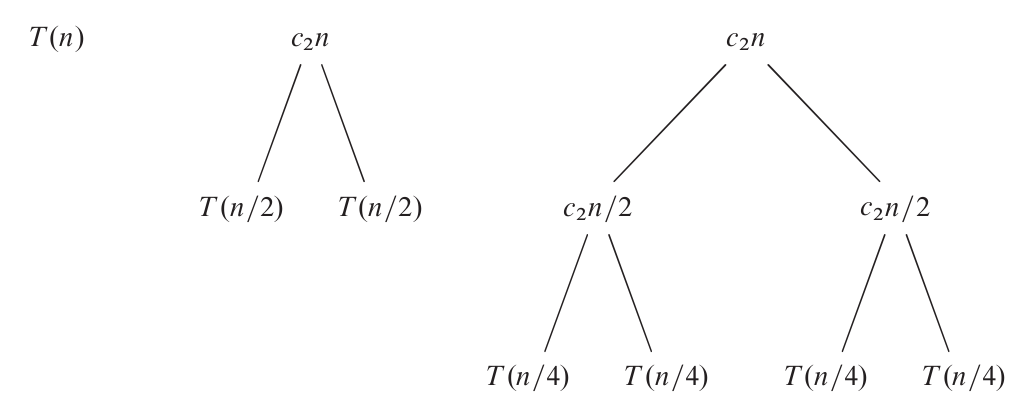
\includegraphics[width=0.5\textwidth]{figs/chap03/merge-sort-analysis1}
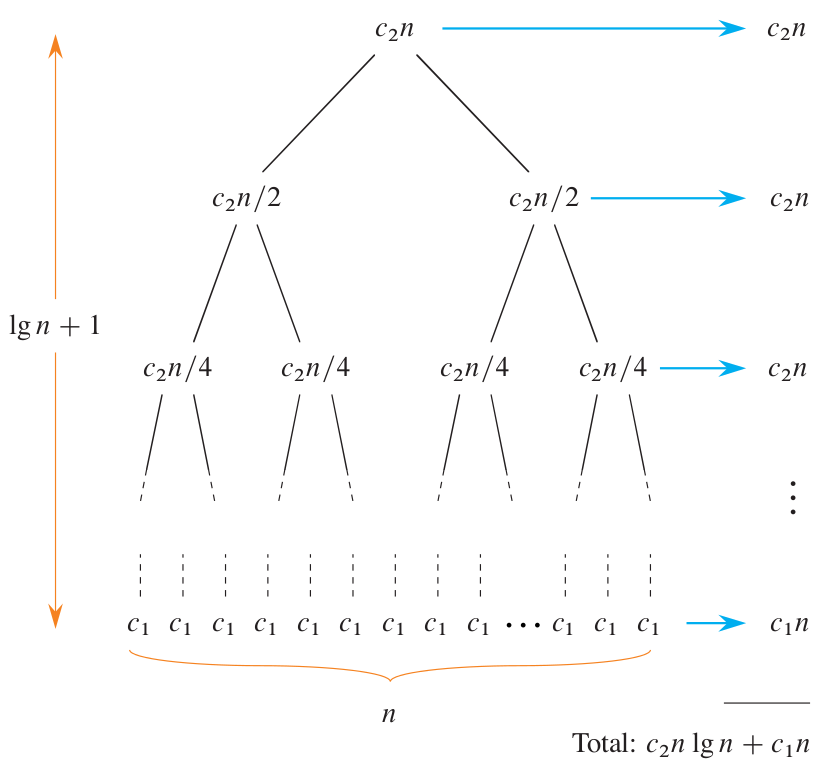
\includegraphics[width=0.4\textwidth]{figs/chap03/merge-sort-analysis2}
\end{figure}
}
\end{itemize}
\end{frame}


\begin{frame}{‌مرتب‌سازی ادغامی}
\begin{itemize}\itemr
\item[-]
مقدار
\m{c_2n}
در ریشهٔ این درخت در واقع زمان مورد نیاز برای تقسیم و ادغام را نشان می‌دهد، هنگامی که اندازهٔ مسئله برابر است با n . دو زیر درخت در سطح ۱ این درخت زمان‌های مورد نیاز را وقتی اندازهٔ ورودی
\m{n/2}
است نشان می‌دهند. هزینه مورد نیاز برای تقسیم و ادغام هر‌کدام از این زیر درخت‌ها برابر است با
\m{c_2n/2}
و مجموعه این هزینه‌ها برای دو زیر درخت برابر است با
\m{c_2n}.
\item[-]
چنانچه این محاسبات را ادامه دهیم، به این نتیجه می‌رسیم که هزینه تقسیم و ادغام برای هر یک از سطوح درخت برابر است با
\m{c_2n}.
\end{itemize}
\end{frame}


\begin{frame}{‌مرتب‌سازی ادغامی}
\begin{itemize}\itemr
\item[-]
سطح آخر، یعنی سطحی که برگ‌های درخت در آن قرار دارد، حالت پایه را نشان می‌دهد که در این حالت زمان اجرای هر یک از زیر آرایه‌ها برابر است با
\m{c_1}
و چون تعداد n زیر آرایه با طول ۱ داریم، زمان اجرا برای کل زیر آرایه‌ها برابر است با
\m{c_1 n}.
\item[-]
از آنجایی که این درخت در هر مرحله به دو بخش تقسیم می‌شود، تعداد سطوح درخت برابر است با
\m{\lg n + 1}.
\item[-]
بنابراین زمان کل اجرای الگوریتم برابر است با
\m{c_2n \lg n+ c_1n} .
\item[-]
می‌توانیم با استفاده از تحلیل مجانبی بنویسیم
\m{T(n) = \ath{n \lg n}}.
\end{itemize}
\end{frame}


\begin{frame}{‌جستجوی دودویی}
\begin{itemize}\itemr
\item[-]
برای جستجوی یک مقدار در یک آرایه باید همهٔ عناصر آرایه را یک‌به‌یک بررسی کنیم. این جستجو برای یک آرایه با
\m{n}
عنصر در زمان
\m{O(n)}
انجام می‌شود.
\item[-]
حال فرض می‌کنیم می‌خواهیم یک مقدار را در یک آرایه مرتب شده پیدا کنیم.
\item[-]
برای این کار می‌توانیم از یک الگوریتم تقسیم و حل به نام جستجوی دودویی
\fn{1}{binary search}
استفاده کنیم.
\end{itemize}
\end{frame}


\begin{frame}{‌جستجوی دودویی}
\begin{itemize}\itemr
\item[-]
الگوریتم تقسیم و حل آرایه را به دو قسمت تقسیم می‌کند. برای جستجوی مقدار
\code{x}
در آرایه
\code{A}
، ابتدا مقدار
\code{x}
با عنصر وسط آرایه یعنی
\code{A[n/2]}
مقایسه می‌شود. اگر
\code{x}
برابر با مقدار وسط آرایه بود، مقدار مورد نظر یافته شده است. اگر
\code{x}
کوچکتر از عنصر وسط آرایه بود، باید
\code{x}
را در نیمه اول آرایه یعنی\\
\code{A[1:n/2-1]}
جستجو کنیم. در غیراینصورت باید
\code{x}
را در نیمه دوم آرایه یعنی
\code{A[n/2+1:n]}
جستجو کنیم. این روند را برای زیر آرایه‌ها ادامه می‌دهیم تا یا
\code{x}
یافته شود یا مشخص شود که
\code{x}
در آرایه وجود ندارد.
\end{itemize}
\end{frame}


\begin{frame}{‌جستجوی دودویی}
\begin{itemize}\itemr
\item[-]
بنابراین مراحل انجام جستجوی دودویی به صورت زیر است.
\item[۱.]
تقسیم : برای پیدا کردن مقدار
\code{x}
در آرایه
\code{A[low:high]}
قرار می‌دهیم
\code{mid=$\lfloor$(low + high)/2$\rfloor$} .
اگر
\code{A[mid]}
برابر با
\code{x}
بود به نتیجه رسیده‌ایم در غیراینصورت آرایه را به دو قسمت
\code{A[low:mid-1]}
و
\code{A[mid+1:high]}
تقسیم می‌کنیم. این تقسیم تنها در صورتی می‌تواند انجام شود که
\code{high}
از
\code{low}
بزرگ‌تر باشد.
\item[۲.]
حل : در صورتی که مقدار
\code{x}
از
\code{A[mid]}
کوچکتر بود، الگوریتم جستجو برای
\code{A[low:mid-1]}
فراخوانی می‌شود، در غیراینصورت برای
\code{A[mid+1:high]}
فراخوانی می‌شود.
\item[۳.]
ترکیب : در گام ترکیب هیچ عملیاتی انجام نمی‌شود.
\end{itemize}
\end{frame}


\begin{frame}{‌جستجوی دودویی}
\begin{itemize}\itemr
\item[-]
برای پیدا کردن عدد ۱۸ در آرایهٔ زیر، الگوریتم به صورت زیر عمل می‌کند.
\begin{figure}
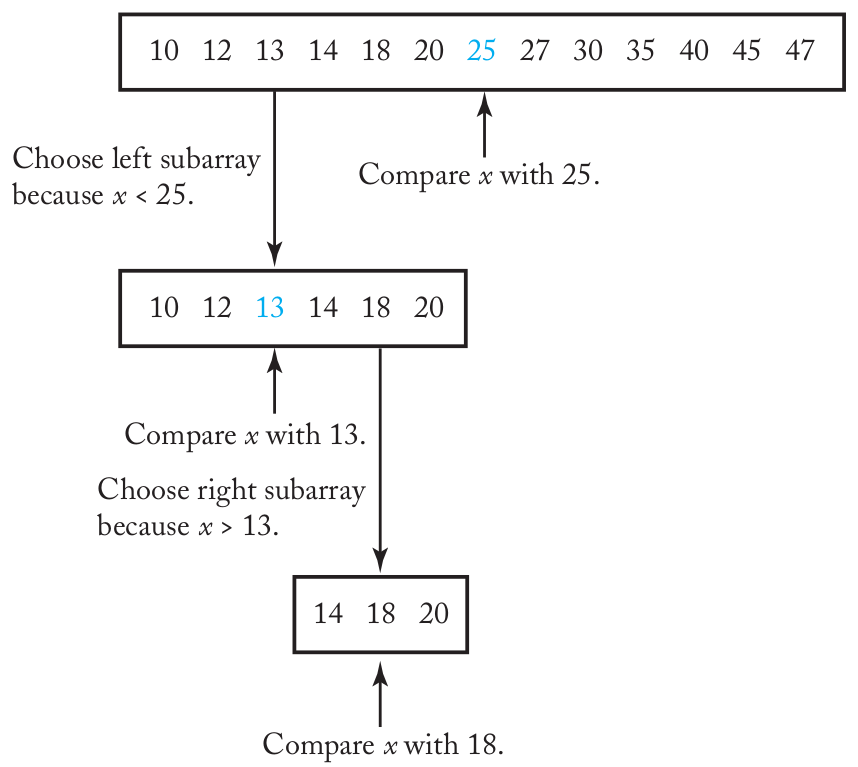
\includegraphics[width=0.55\textwidth]{figs/chap03/binarysearch2-1}
\end{figure}
\end{itemize}
\end{frame}


\begin{frame}{‌جستجوی دودویی}
\begin{itemize}\itemr
\item[-]
الگوریتم جستجوی دودویی به صورت زیر است.
\begin{algorithm}[H]\alglr
  \caption{‌Binary Search} 
  \begin{algorithmic}[1]
   \Func{BinarySearch}{A, x, low, high}
   \If{(low > high)}
        \State \Return -‌1
    \EndIf
    \State mid = $\lfloor$(low + high)/2$\rfloor$
    \If{(x == A[mid])}
         \State \Return mid
     \EndIf
     \If{(x < A[mid])}
          \State \Return BinarySearch (A, x, low, mid-1)
      \Else
          \State \Return BinarySearch (A, x, mid+1, high)
      \EndIf                          
  \end{algorithmic}
  \label{alg:merge}
\end{algorithm}
\item[-]
برای جستجوی مقدار
\code{x}
جستجوی دودویی باید به صورت
\code{BinarySearch(A, x, 1, n)}
فراخوانی شود.
\end{itemize}
\end{frame}



\begin{frame}{‌جستجوی دودویی}
\begin{itemize}\itemr
\item[-]
در تقسیم یک آرایه به دو قسمت صرفا یک عملیات تقسیم انجام می‌شود. بنابراین
\m{D(n) = O(1)}
. تقسیم آرایه در زمان ثابت انجام می‌شود.
\item[-]
بنابراین زمان اجرای الگوریتم جستجوی دودویی برای آرایه با
\m{n}
عنصر برابر است با زمان اجرای الگوریتم برای آرایه‌ای با
\m{n/2}
عنصر به علاوه یک زمان ثابت.
\item[-]
می‌توانیم بنویسیم
\m{T(n) = T(\frac{n}{2}) + O(1)}
و
\m{T(1) = 1}
\item[-]
با حل این رابطه بازگشتی به دست می‌آوریم
\m{T(n) = O(\lg n)}.
\end{itemize}
\end{frame}


\begin{frame}{‌مرتب‌سازی سریع}
\begin{itemize}\itemr
\item[-]
یکی از الگوریتم‌های مرتب‌سازی بسیار پر استفاده الگوریتم مرتب‌سازی سریع
\fn{1}{quicksort algorithm}
است.
\item[-]
این الگوریتم یک الگوریتم تقسیم و حل است. زمان اجرای آن در بدترین حالت
\ath{n^2}
است، اما در حالت میانگین در زمان
\ath{n \lg n}
اجرا می‌شود. این الگوریتم به حافظه اضافی نیاز ندارد.
\end{itemize}
\end{frame}


\begin{frame}{‌مرتب‌سازی سریع}
\begin{itemize}\itemr
\item[-]
برای مرتب‌سازی آرایه
\code{A[p:r]}
این الگوریتم از روش تقسیم و حل به صورت زیر استفاده می‌کند.
\item[۱.]
تقسیم : آرایهٔ
\code{A[p:r]}
به دو قسمت
\code{A[p:q-1]}
(قسمت پایین)
\fn{1}{low side}
و
\code{A[q+1:r]}
(قسمت بالا)
\fn{2}{high side}
تقسیم می‌شود به طوری که همه عناصر قسمت پایین از عنصر
\code{A[q]}
(عنصر محور)
\fn{3}{pivot}
کوچکتر یا برابرند و عناصر قسمت بالا از عنصر محور بزرگ‌ترند.
\item[۲.]
حل : الگوریتم مرتب‌سازی سریع برای دو زیر آرایه
\code{A[p:q-1]}
و
\code{A[q+1:r]}
فراخوانی می‌شود.
\item[۳.]
ترکیب : در این قسمت هیچ عملیاتی انجام نمی‌شود. از آنجایی که همه عناصر
\code{A[p:q-1]}
مرتب شده و کوچکتر یا مساوی
\code{A[q]}
هستند و همهٔ عناصر
\code{A[q+1:r]}
مرتب شده و بزرگتر از
\code{A[q]}
هستند، بنابراین کل آرایه
\code{A[p:r]}
مرتب شده است.
\end{itemize}
\end{frame}

\begin{frame}{‌مرتب‌سازی سریع}
\begin{itemize}\itemr
\item[-]
در تقسیم آرایه به دو قسمت پایین و بالا، فرض کنید قسمت کرمی رنگ در شکل زیر عناصری باشند که مقدار آنها از عنصر محوری x کمتر و قسمت آبی رنگ عناصری باشند که مقدار آنها از عنصر محوری بیشتر است.
\begin{figure}
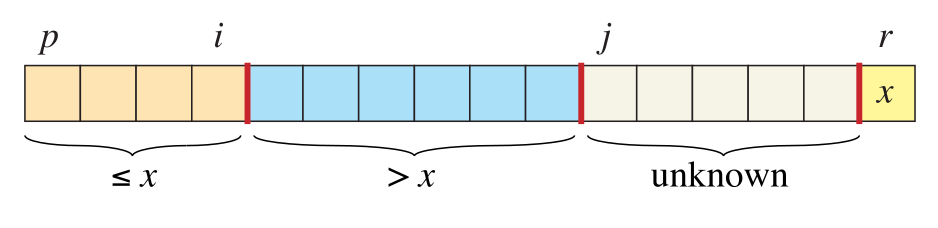
\includegraphics[width=0.7\textwidth]{figs/chap03/quicksort1}
\end{figure}
\end{itemize}
\end{frame}


\begin{frame}{‌مرتب‌سازی سریع}
\begin{itemize}\itemr
\item[-]
اندیس i مرز بین قسمت پایین و قسمت بالا را نگهداری می‌کند. توسط اندیس j عناصر آرایه یک به یک بررسی می‌شوند. در صورتی که مقدار آنها از عنصر محوری x کمتر باشد به صورت زیر به قسمت پایین منتقل می‌شوند و مرز قسمت پایین و بالا تغییر می‌کند، در غیر اینصورت قسمت در مکان خود نگه داشته می‌شوند.
\begin{figure}
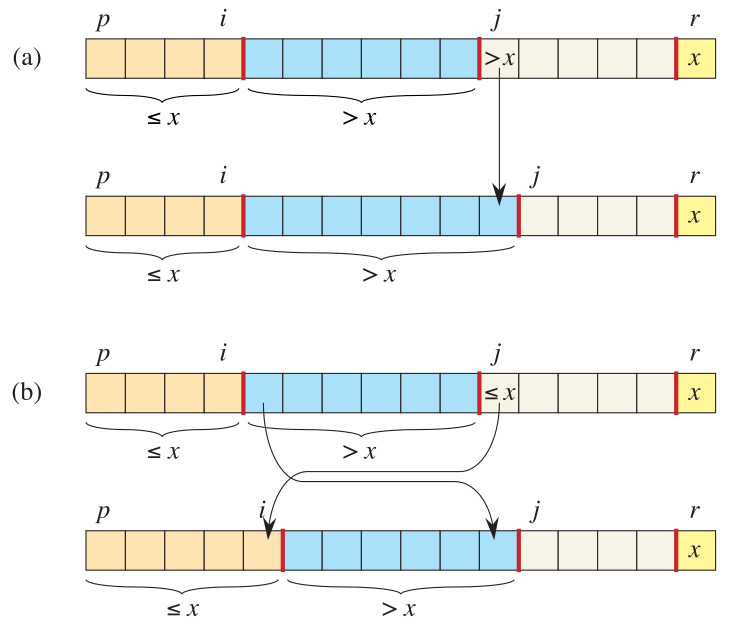
\includegraphics[width=0.5\textwidth]{figs/chap03/quicksort2}
\end{figure}
\end{itemize}
\end{frame}


\begin{frame}{‌مرتب‌سازی سریع}
\begin{itemize}\itemr
\item[-]
در شکل زیر نحوه اجرای الگوریتم تقسیم‌بندی نشان داده شده است. عنصر محور در اینجا برابر است با
\code{A[r]}.
\begin{figure}
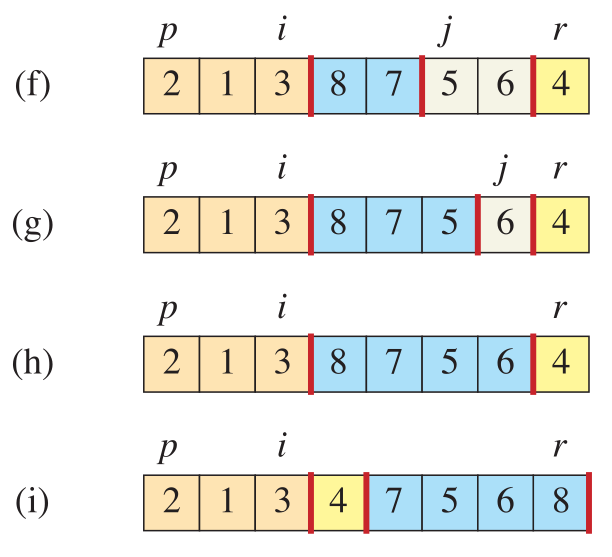
\includegraphics[width=0.4\textwidth]{figs/chap03/partition2}
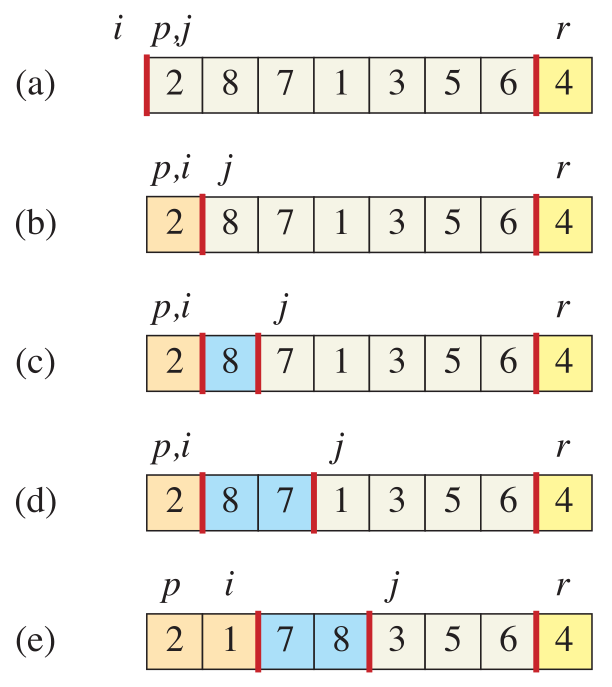
\includegraphics[width=0.4\textwidth]{figs/chap03/partition1}
\end{figure}
\end{itemize}
\end{frame}



\begin{frame}{‌مرتب‌سازی سریع}
\begin{itemize}\itemr
\item[-]
الگوریتم مرتب‌سازی سریع به صورت زیر است.
\begin{algorithm}[H]\alglr
  \caption{Quicksort} 
  \begin{algorithmic}[1]
   \Func{Quicksort}{A, p, r}
   \If{p < r}
           \LeftComment{Partition the subarray around the pivot, which ends up in A[q].}
           \State q = Partition (A, p, r)
           \State Quicksort (A, p, q-1) \LeftComment{recursively sort the low side}
           \State Quicksort (A, q+1, r) \LeftComment{recursively sort the high side}
    \EndIf                           
  \end{algorithmic}
  \label{alg:merge}
\end{algorithm}
\end{itemize}
\end{frame}


\begin{frame}{‌مرتب‌سازی سریع}
\begin{itemize}\itemr
\item[-]
الگوریتم تقسیم‌بندی
\fn{1}{partition}
باید عناصر آرایه را به گونه‌ای جابجا کند که همهٔ عناصر قسمت پایین از عنصر محور کوچک‌تر یا مساوی و عناصر قسمت بالا از عنصر محور بزرگ‌تر باشند.
\end{itemize}
\end{frame}


\begin{frame}{‌مرتب‌سازی سریع}
\begin{itemize}\itemr
\item[-]
الگوریتم تقسیم بندی به صورت زیر است.
\begin{algorithm}[H]\alglr
  \caption{Partition} 
  \begin{algorithmic}[1]
   \Func{Partition}{A, p, r}
   \State x = A[r] \LeftComment{the pivot}
   \State i = p - 1 \LeftComment{highest index into the low side}
   \For{j = p \To r-1} \LeftComment{process each element other than the pivot}
        \If{A[j] <= x} \LeftComment{does this element belong on the low side?}
            \State i = i+1 \LeftComment{index of a new slot in the low side}
            \State exchange A[i] with A[j] \LeftComment{put this element there}
        \EndIf
   \EndFor 
   \State exchange A[i+1] with A[r] \LeftComment{pivot goes just to the right of the low side}
   \State \Return i+1 \LeftComment{new index of the pivot}
  \end{algorithmic}
  \label{alg:merge}
\end{algorithm}
\end{itemize}
\end{frame}


\begin{frame}{‌مرتب‌سازی سریع}
\begin{itemize}\itemr
\item[-]
زمان اجرای الگوریتم مرتب‌سازی سریع به نحوه تقسیم‌بندی آرایه بستگی دارد. اگر تقسیم‌بندی آرایه متوازن نباشد الگوریتم در زمان
\ath{n^2}
اجرا می‌شود اما اگر تقسیم‌بندی متوازن باشد، الگوریتم در زمان
\ath{n \lg n}
اجرا می‌شود.
\end{itemize}
\end{frame}


\begin{frame}{‌مرتب‌سازی سریع}
\begin{itemize}\itemr
\item[-]
اگر در هر بار تقسیم‌بندی آرایه، یک قسمت
\m{n-1}
عنصر و قسمت دیگر
\m{0}
عنصر داشته باشد، آنگاه تقسیم‌بندی نامتوازن است. هزینه تقسیم‌بندی آرایه برابراست با
\ath{n}
. مرتب‌سازی یک آرایه با صفر عنصر در زمان ثابت انجام می‌شود یعنی
\m{T(0) = \ath{1}}
بنابراین خواهیم داشت :
\begin{align*}
\m{T(n) = T(n-1) + T(0) + \ath{n} = T(n-1) + \ath{n}}
\end{align*}
\item[-]
با حل کردن این رابطه بازگشتی به دست می‌آوریم
\m{T(n) = \ath{n^2}}.
\item[-]
بنابراین در بدترین حالت الگوریتم مرتب‌سازی سریع مانند مرتب‌سازی درجی عمل می‌کند. بدترین حالت در مرتب‌سازی سریع وقتی رخ می‌دهد که آرایه کاملا مرتب باشد.
\end{itemize}
\end{frame}


\begin{frame}{‌مرتب‌سازی سریع}
\begin{itemize}\itemr
\item[-]
اگر الگوریتم تقسیم‌بندی، آرایه را به دو قسمت مساوی تقسیم کند، آنگاه می‌توانیم زمان اجرای الگوریتم را با استفاده از رابطه بازگشتی زیر محاسبه کنیم.
\begin{align*}
\m{T(n) = 2 T(n/2) + \ath{n}}
\end{align*}
\item[-]
با حل این رابطه به دست می‌آوریم
\m{T(n) = \ath{n \lg n}}.
\item[-]
می‌توان اثبات کرد که الگوریتم مرتب‌سازی سریع در حالت میانگین در زمان
\ath{n \lg n}
اجرا می‌شود.
حالت میانگین وقتی است که در الگوریتم تقسیم‌بندی، آرایه به طور میانگین با یک نسبت معین به دو قسمت تقسیم شود.
\end{itemize}
\end{frame}



\begin{frame}{‌مرتب‌سازی سریع}
\begin{itemize}\itemr
\item[-]
همچنین برای اینکه بدترین حالت اتفاق نیافتد، می‌توان عنصر محوری را به صورت تصادفی انتخاب کرد و اثبات کرد که در این صورت زمان اجرای الگوریتم مرتب‌سازی سریع
\ath{n \lg n}
خواهد بود.
\item[-]
یک روش دیگر برای اینکه بدترین حالت اتفاق نیافتد این است که بین اولین عنصر، آخرین عنصر، و عنصر وسط از آرایه، عنصری که مقدار آن میانهٔ دو مقدار دیگر است را به عنوان عنصر محوری انتخاب کنیم. این روش به استراتژی انتخاب میانهٔ سه مقدار 
\fn{1}{median of three values}
معروف است.
\end{itemize}
\end{frame}

\begin{frame}{‌ضرب ماتریس‌ها}
\begin{itemize}\itemr
\item[-]
از روش تقسیم و حل می‌توانیم برای ضرب ماتریس‌های مربعی استفاده کنیم.
\item[-]
فرض کنید
\m{A = (a_{ij})}
و
\m{B = (b_{ij})}
دو ماتریس
\m{n \times n}
باشند. ماتریس
\m{C = A \cdot B}
نیز یک ماتریس
\m{n \times n}
است که درایه‌های آن به صورت زیر محاسبه می‌شوند.
\begin{flushleft}
\m{c_{ij} = \sum_{k=1}^{n} a_{ik} \cdot b_{kj}}
\end{flushleft}
\end{itemize}
\end{frame}


\begin{frame}{‌ضرب ماتریس‌ها}
\begin{itemize}\itemr
\item[-]
الگوریتم ضرب دو ماتریس در زیر نوشته شده‌است.
\begin{algorithm}[H]\alglr
  \caption{Matrix} 
  \begin{algorithmic}[1]
    \Func{Matrix-Multiply}{A, B, C, n}
       \For{i = 1 \To n} \LeftComment{compute entries in each of n rows}
           \For{j = 1 \To n} \LeftComment{compute n entries in row i}
			   \For{k = 1 \To n}
					\State c[i,j] = c[i,j] + a[i,k] * b[k,j] \LeftComment{compute c[i,j]}
			    \EndFor
			\EndFor
	   \EndFor 
     \end{algorithmic}
  \label{alg:merge}
\end{algorithm}
\item[-]
از آنجایی که خط ۴ باید
\m{n^3}
بار تکرار شود، بنابراین زمان مورد نیاز برای اجرای این الگوریتم برابر است با
\ath{n^3}.
\end{itemize}
\end{frame}

\begin{frame}{‌ضرب ماتریس‌ها}
\begin{itemize}\itemr
\item[-]
حال می‌خواهیم ضرب دو ماتریس را توسط روش تقسیم و حل محاسبه کنیم.
\item[-]
در مرحله تقسیم، یک ماتریس
\m{n \times n}
را به چهار ماتریس
\m{n/2 \times n/2}
تقسیم می‌کنیم. برای سادگی فرض می‌کنیم n توانی از ۲ باشد و امکان تقسیم کردن آن به ۲ در فرایند الگوریتم تقسیم و حل وجود داشته باشد.
\end{itemize}
\end{frame}


\begin{frame}{‌ضرب ماتریس‌ها}
\begin{itemize}\itemr
\item[-]
با فرض اینکه هر یک از ماتریس‌های
A
,
B
و
C
را به چهار قسمت تقسیم کنیم، محاسبات به صورت زیر انجام می‌شود.
\begin{align*}
\m{C = A \cdot B \Rightarrow} \left( \begin{array}{cc} \m{C_{11}} & \m{C_{12}} \\ \m{C_{21}} & \m{C_{22}} \end{array} \right)
= \left( \begin{array}{cc} \m{A_{11}} & \m{A_{12}} \\ \m{A_{21}} & \m{A_{22}} \end{array} \right)
\left( \begin{array}{cc} \m{B_{11}} & \m{B_{12}} \\ \m{B_{21}} & \m{B_{22}} \end{array} \right)
\end{align*}
\item[-]
بنابراین خواهیم داشت :
\begin{align*}
\m{C_{11} = A_{11} \cdot B_{11} + A_{12} \cdot B_{21}}\\
\m{C_{12}= A_{11} \cdot B_{12} + A_{12} \cdot B_{22}}\\
\m{C_{21}= A_{21} \cdot B_{11} + A_{22} \cdot B_{21}}\\
\m{C_{22}= A_{21} \cdot B_{12} + A_{22} \cdot B_{22}}
\end{align*}
\end{itemize}
\end{frame}



\begin{frame}{‌ضرب ماتریس‌ها}
\begin{itemize}\itemr
\item[-]
بنابراین ضرب یک جفت ماتریس 
\m{n \times n}
را به ضرب هشت جفت ماتریس 
\m{n/2 \times n/2}
تبدیل کردیم.
\item[-]
توجه کنید که در این محاسبات نتیجهٔ ضرب
\m{A_{11} \cdot B_{11}}
و همچنین
\m{A_{12} \cdot B_{21}}
باید در 
\m{C_{11}}
ذخیره شود.
\begin{align*}
\m{C_{11} = A_{11} \cdot B_{11} + A_{12} \cdot B_{21}}\\
\m{C_{12}= A_{11} \cdot B_{12} + A_{12} \cdot B_{22}}\\
\m{C_{21}= A_{21} \cdot B_{11} + A_{22} \cdot B_{21}}\\
\m{C_{22}= A_{21} \cdot B_{12} + A_{22} \cdot B_{22}}
\end{align*}
\item[-]
حالت پایه در این الگوریتم وقتی است که می خواهیم دو ماتریس
\m{1 \times 1}
را در هم ضرب کنیم که در این حالت در واقع دو عدد را در هم ضرب می‌کنیم.
\end{itemize}
\end{frame}


\begin{frame}{‌ضرب ماتریس‌ها}
\begin{itemize}\itemr
\item[-]
الگوریتم تقسیم و حل برای ضرب دو ماتریس را می‌توانیم به صورت زیر بنویسیم.
\begin{algorithm}[H]\alglr
  \caption{Matrix} 
  \begin{algorithmic}[1]
    \Func{Matrix-Multiply-Recursive}{A, B, C, n}
   \Statex \LeftComment{Base case.}    
    \If{n==1}
    	\State \mc{c_{11}} = \mc{c_{11}} + \mc{a_{11}} * \mc{b_{11}}
    	\State \Return
    \EndIf
   \Statex \LeftComment{Divide.}
   \State Partition A, B, and C into n/2 \mc{\times} n/2 submatrices 
    	\Statex \mc{A_{11}, A_{12}, A_{21}, A_{22}}; 
    	\Statex \mc{B_{11}, B_{12}, B_{21}, B_{22}};
    	\Statex \mc{C_{11}, C_{12}, C_{21}, C_{22}}; respectively    
  \end{algorithmic}
  \label{alg:merge}
\end{algorithm}
\end{itemize}
\end{frame}


\begin{frame}{‌ضرب ماتریس‌ها}
\begin{itemize}\itemr
\item[-]
\begin{algorithm}[H]\alglr
  \caption{Matrix} 
  \begin{algorithmic}[1]
    \setcounter{ALG@line}{4}
   \Statex \LeftComment{Conquer.}   
    	\State Matrix-Multiply-Recursive (\mc{A_{11}, B_{11}, C_{11}, n/2})
    	\State Matrix-Multiply-Recursive (\mc{A_{11}, B_{12}, C_{12}, n/2})
    	\State Matrix-Multiply-Recursive (\mc{A_{21}, B_{11}, C_{21}, n/2})
    	\State Matrix-Multiply-Recursive (\mc{A_{21}, B_{12}, C_{22}, n/2})
    	\State Matrix-Multiply-Recursive (\mc{A_{12}, B_{21}, C_{11}, n/2})
    	\State Matrix-Multiply-Recursive (\mc{A_{12}, B_{22}, C_{12}, n/2})
    	\State Matrix-Multiply-Recursive (\mc{A_{22}, B_{21}, C_{21}, n/2})
    	\State Matrix-Multiply-Recursive (\mc{A_{22}, B_{22}, C_{22}, n/2})
  \end{algorithmic}
  \label{alg:merge}
\end{algorithm}
\end{itemize}
\end{frame}


\begin{frame}{‌ضرب ماتریس‌ها}
\begin{itemize}\itemr
\item[-]
یک ضرب ماتریسی با اندازهٔ 
\m{n}
 را به ۸ ضرب ماتریسی با اندازهٔ 
\m{n/2}
تبدیل کردیم.
\item[-]
فرض می‌کنیم که در تقسیم ماتریس به ماتریس‌های کوچک‌تر، تنها اندیس‌ها را نامگذاری مجدد می‌کنیم و بنابراین عملیات در زمان ثابت می‌تواند انجام شود.
\item[-]
بنابراین برای تحلیل این الگوریتم، می‌توانیم از رابطه بازگشتی زیر استفاده کنیم.
\begin{center}
\m{T(n) = 8 T(n/2) +  \ath{1}}
\end{center}
\end{itemize}
\end{frame}


\begin{frame}{‌ضرب ماتریس‌ها}
\begin{itemize}\itemr
\item[-]
با حل کردن این معادله به دست می‌آوریم
\m{T(n) = \ath{n^3}}.
\item[-]
بنابراین روش تقسیم و حل زمان محاسبات را در ضرب ماتریسی کاهش نمی‌دهد.
\item[-]
با استفاده از الگوریتم استراسن
\fn{1}{Strassen}
که از یک الگوریتم تقسیم و حل بهینه‌تر استفاده می‌کند، زمان محاسبات کاهش پیدا خواهد کرد.
\end{itemize}
\end{frame}

\begin{frame}{‌الگوریتم استراسن}
\begin{itemize}\itemr
\item[-]
ضرب دو ماتریس
\m{n \times n}
را در زمان کمتر از
\m{n^3}
نیز می‌توان انجام داد. از آنجایی که برای ضرب دو ماتریس مربعی با اندازهٔ n دقیقا به
\m{n^3}
گام محاسباتی نیاز است،‌ بسیاری بر این باور بودند که ضرب ماتریسی نمی‌تواند در زمانی کمتر صورت بگیرد تا اینکه در سال ۱۹۶۹ ولکر استراسن
\fn{1}{Volker Strassen}
 ریاضیدان آلمانی، الگوریتمی با زمان اجرای
\ath{n^{\lg 7}}
ابداع کرد. از آنجایی که
\m{\lg 7 = 2.8073 ...}
، بنابراین می‌توان گفت الگوریتم استراسن در زمان
\abo{n^{2.81}}
ضرب دو ماتریس را محاسبه می‌کند.
\item[-]
الگوریتم استراسن یک الگوریتم از نوع و تقسیم و حل است.
\item[-]
استراسن مجددا در سال ۱۹۸۶ الگوریتمی از مرتبه
\abo{n^{2.48}}
ارائه داد.
در سال ۱۹۹۰ الگوریتمی از مرتبه
\abo{n^{2.38}}
و در سال ۲۰۲۳ یک الگوریتم بهبود یافته ارائه شد.
 جستجو برای پیدا کردن سریع‌ترین الگوریتم ضرب ماتریسی همچنان ادامه دارد.
\end{itemize}
\end{frame}


\begin{frame}{‌الگوریتم استراسن}
\begin{itemize}\itemr
\item[-]
ایدهٔ الگوریتم استراسن این است که در مراحل تقسیم و ترکیب از عملیات بیشتری استفاده می‌کند و بنابراین مراحل تقسیم و ترکیب در این الگوریتم نسبت به مراحل تقسیم و ترکیب در الگوریتم تقسیم و حل عادی زمان بیشتری صرف می‌کند ولی در ازای این افزایش زمان، در مرحله حل بازگشتی زمان کمتری مصرف می‌شود. در واقع در مرحله بازگشتی به جای فراخوانی ۸ تابع بازگشتی ۷ تابع بازگشتی فراخوانی می‌شوند.
\item[-]
به عبارت دیگر عملیات مورد نیاز برای یکی از فراخوانی‌های بازگشتی توسط تعدادی عملیات جمع در مراحل تقسیم و ترکیب انجام می‌شود.
\end{itemize}
\end{frame}


\begin{frame}{‌الگوریتم استراسن}
\begin{itemize}\itemr
\item[-]
به عنوان مثال فرض کنید می‌خواهیم به ازای دو عدد دلخواه 
\m{x}
 و 
\m{y}
  ، مقدار
\m{x^2 - y^2}
را محاسبه کنیم. اگر بخواهیم این محاسبات را به صورت معمولی انجام دهیم، باید ابتدا x و y را به توان ۲ برسانیم و سپس دو مقدار به دست آمده را از هم کم کنیم. اما یک روش دیگر برای این محاسبات وجود دارد.
\item[-]
می‌دانیم
\m{x^2 - y^2 = (x+y)(x-y)}
، بنابراین می‌توانیم این محاسبات را با یک عمل ضرب و دو عمل جمع و تفریق انجام دهبم. اگر x و y دو عدد باشند،‌ زمان انجام محاسبات تفاوت چندانی نخواهد کرد، اما اگر x و y دو ماتریس بزرگ باشند، یک عمل ضرب کمتر بهبود زیادی در زمان اجرا ایجاد می‌کند.
\item[-]
توجه کنید که جمع دو ماتریس مربعی با اندازهٔ n در زمان 
\m{O(n^2)}
انجام می‌شود، و ضرب دو ماتریس در زمان
\m{O(n^3)} .
\end{itemize}
\end{frame}


\begin{frame}{‌الگوریتم استراسن}
\begin{itemize}\itemr
\item[-]
حال که با ایدهٔ الگوریتم استراسن آشنا شدیم، الگوریتم را بررسی می‌کنیم.\\
۱. اگر
\m{n=1}
، آنگاه هر ماتریس تنها یک درایه دارد. در این صورت باید یک عملیات ضرب ساده انجام داد که در زمان
\ath{1}
امکان پذیر است. اگر
\m{n \neq 1}
، آنگاه هر یک از ماتریس‌های ورودی
\m{A}
و
\m{B}
 را به چهار ماتریس
\m{n/2 \times n/2}
تقسیم می‌کنیم. این عملیات نیز در
\ath{1}
امکان پذیر است.\\
۲. با استفاده از زیر ماتریس‌های به دست آمده از مرحله قبل تعداد ۱۰ ماتریس
\m{S_1, S_2, ..., S_{10}}
محاسبه می‌شوند. این عملیات در زمان
\ath{n^2}
انجام می‌شود.\\
۳. تابع ضرب ماتریسی به تعداد ۷ بار بر روی ماتریس‌های
\m{S_i}, \m{A_{ij}}, \m{B_{ij}}
که ابعاد هر کدام 
\m{n/2 \times n/2}
است، به طور بازگشتی انجام می‌شود. نتیجهٔ این محاسبات در ۷ ماتریس
\m{P_1, P_2, ..., P_7}
ذخیره می‌شود.
عملیات این مرحله در زمان
\m{7 T(n/2)}
انجام می‌شود.\\
۴. با استفاده از ماتریس‌های
\m{P_1, P_2, ..., P_7}
، ماتریس‌های
\m{C_{11}, C_{12}, C_{21}, C_{22}}
محاسبه می‌شود. این عملیات نیز در زمان
\ath{n^2}
انجام می‌شود.
\end{itemize}
\end{frame}


\begin{frame}{‌الگوریتم استراسن}
\begin{itemize}\itemr
\item[-]
بنابراین  زمان کل مورد نیاز برای الگوریتم استراسن از رابطه بازگشتی زیر به دست می‌آید.
\begin{flushleft}
\m{T(n) = 7 T(n/2) + \ath{n^2}}
\end{flushleft}
\item[-]
با حل این رابطه بازگشتی به دست می‌آوریم :
\begin{flushleft}
\m{T(n) = \ath{n^{\lg 7}} = O(n^{2.81})}
\end{flushleft}
\end{itemize}
\end{frame}


\begin{frame}{‌الگوریتم استراسن}
\begin{itemize}\itemr
\item[-]
حال ببینیم ماتریس‌های
\m{P_k}
چگونه با استفاده از ماتریس‌های
\m{A_{ij}}
و
\m{B_{ij}}
محاسبه می‌شوند.
\end{itemize}
\end{frame}


\begin{frame}{‌الگوریتم استراسن}
\begin{itemize}\itemr
\item[-]
در مرحلهٔ اول تعداد ۱۰ ماتریس 
\m{S_i}
 به صورت زیر محاسبه می‌شوند.
\begin{align*}
&\m{S_1 = B_{12} - B_{22}}\\
&\m{S_2 = A_{11} + A_{12}}\\
&\m{S_3 = A_{21} + A_{22}}\\
&\m{S_4 = B_{21} - B_{11}}\\
&\m{S_5 = A_{11} + A_{22}}\\
&\m{S_6 = B_{11} + B_{22}}\\
&\m{S_7 = A_{12} - A_{22}}\\
&\m{S_8 = B_{21} + B_{22}}\\
&\m{S_9 = A_{11} - A_{21}}\\
&\m{S_{10} = B_{11} + B_{12}}\\
\end{align*}
\end{itemize}
\end{frame}


\begin{frame}{‌الگوریتم استراسن}
\begin{itemize}\itemr
\item[-]
در محاسبات فوق ۱۰ بار ماتریس‌های
\m{n/2 \times n/2}
را با هم جمع کردیم که این عملیات در زمان
\ath{n^2}
امکان پذیر است.
\end{itemize}
\end{frame}


\begin{frame}{‌الگوریتم استراسن}
\begin{itemize}\itemr
\item[-]
در مرحلهٔ بعد ۷ ماتریس 
\m{P_i}
 را با استفاده از زیر ماتریس‌های 
\m{A_{ij}}
  و 
\m{B_{ij}}
   و ماتریس‌های 
\m{S_i}
    بدست می‌آوریم.
\begin{align*}
&\m{P_1 = A_{11} \cdot S_1 (= A_{11} \cdot B_{12} - A_{11} \cdot B_{22})}\\
&\m{P_2 = S_2 \cdot B_{22} (= A_{11} \cdot B_{22} + A_{12} \cdot B_{22})} \\
&\m{P_3 = S_3 \cdot B_{11} (= A_{21} \cdot B_{11} + A_{22} \cdot B_{11})}\\
&\m{P_4 = A_{22} \cdot S_4 (= A_{22} \cdot B_{21} - A_{22} \cdot B_{11})}\\
&\m{P_5 = S_5 \cdot S_6 (= A_{11} \cdot B_{11} + A_{11} \cdot B_{22} + A_{22} \cdot B_{11} + A_{22} \cdot B_{22})}\\
&\m{P_6 = S_7 \cdot S_8 (= A_{12} \cdot B_{21} + A_{12} \cdot B_{22} - A_{22} \cdot B_{21} - A_{22} \cdot B_{22})}\\
&\m{P_7 = S_9 \cdot S_{10} (= A_{11} \cdot B_{11} + A_{11} \cdot B_{12} - A_{21} \cdot B_{11} - A_{21} \cdot B_{12})}
\end{align*}
\end{itemize}
\end{frame}


\begin{frame}{‌الگوریتم استراسن}
\begin{itemize}\itemr
\item[-]
بنابراین در اینجا به ۷ عملیات ضرب نیاز داریم که به صورت بازگشتی انجام می‌شوند.
\item[-]
در مرحلهٔ آخر باید زیر ماتریس‌های 
\m{C_{ij}}
 را با استفاده از ماتریس‌های 
\m{P_i}
  به دست آوریم.
\item[-]
این محاسبات به صورت زیر انجام می‌شوند.
\begin{align*}
&\m{C_{11} = P_5 + P_4 - P_2 + P_6}\\
&\m{C_{12} = P_1 + P_2}\\
&\m{C_{21} = P_3 + P_4}\\
&\m{C_{22} = P_5 + P_1 - P_3 - P_7}
\end{align*}
\end{itemize}
\end{frame}


\begin{frame}{‌الگوریتم استراسن}
\begin{itemize}\itemr
\item[-]
با بسط دادن این روابط می‌توانیم
\m{C_{ij}}
ها را بر اساس
\m{A_{ij}}
و
\m{B_{ij}}
ها به دست آوریم و نشان دهیم که عملیات ضرب به درستی انجام می‌شود.
\begin{align*}
&\m{C_{11} = P_5 + P_4 - P_2 + P_6 (= A_{11} \cdot B_{11} + A_{12} \cdot B_{21})}\\
&\m{C_{12} = P_1 + P_2 (= A_{11} \cdot B_{12} + A_{12} \cdot B_{22})}\\
&\m{C_{21} = P_3 + P_4 (= A_{21} \cdot B_{11} + A_{22} \cdot B_{21})}\\
&\m{C_{22} = P_5 + P_1 - P_3 - P_7 (= A_{21} \cdot B_{12} + A_{22} \cdot B_{22})}
\end{align*}
\item[-]
در مرحله آخر تنها از عملیات جمع استفاده می‌کنیم بنابراین محاسبهٔ
\m{C_{ij}}
ها در زمان
\ath{n^2}
انجام می‌پذیرد.
\end{itemize}
\end{frame}


\begin{frame}{‌الگوریتم استراسن}
\begin{itemize}\itemr
\item[-]
دقت کنید که در این روش
در صورتی که تعداد سطرها یا ستون‌های یک ماتریس فرد باشند، می‌توان یک سطر با مقادیر صفر و یا یک ستون با مقادیر صفر به ماتریس اضافه کرد و پس از انجام عملیات ضرب سطر و ستون با مقادیر صفر را حذف کرد.
\end{itemize}
\end{frame}

\begin{frame}{‌ضرب اعداد}
\begin{itemize}\itemr
\item[-]
می‌خواهیم حاصلضرب دو عدد
\m{u}
و
\m{v}
را محاسبه کنیم.
\item[-]
با استفاده از روش تقسیم و حل، هریک از اعداد را به دو قسمت تقسیم کرده و با استفاده از حاصل‌ضرب قسمت‌های کوچک‌تر، ضرب دو عدد را محاسبه می‌کنیم.
\item[-]
اگر عدد
\m{u}
یک عدد
\m{n}
رقمی باشد می‌توانیم بنویسیم :
\begin{align*}
\m{u = x \times 10^m + y}
\end{align*}
به طوری که
\m{m = \lfloor \frac{n}{2} \rfloor}
است و
\m{x}
یک عدد
\m{\lceil \frac{n}{2} \rceil}
رقمی و
\m{y}
یک عدد
\m{\lfloor \frac{n}{2} \rfloor}
رقمی است.
\end{itemize}
\end{frame}


\begin{frame}{‌ضرب اعداد}
\begin{itemize}\itemr
\item[-]
اگر دو عدد
\m{n}
رقمی
\m{u}
و
\m{v}
داشته باشیم، می‌توانیم بنویسیم :
\begin{align*}
& \m{u = x \times 10^m + y}\\
& \m{v = w \times 10^m + z}
\end{align*}
\item[-]
ضرب این دو عدد برابر است با :
\begin{align*}
& \m{uv = (x \times 10^m + y)(w \times 10^m + z)}\\
& \m{~~~~= xw \times 10^{2m} + (xz + yw) \times 10^m + yz}
\end{align*}
\item[-]
حال برای ضرب دو عدد با اندازه
\m{n}
باید ۴ ضرب برروی اعدادی با اندازه
\m{\frac{n}{2}}
انجام دهیم.
\end{itemize}
\end{frame}


\begin{frame}{‌ضرب اعداد}
\begin{itemize}\itemr
\item[-]
عملیات جمع در زمان خطی انجام می‌شود، بنابراین پیچیدگی زمانی ضرب دو عدد با استفاده از تقسیم و حل برابر است با :
\begin{align*}
\m{T(n) = 4 T(\frac{n}{2}) + O(n)}
\end{align*}
\item[-]
با حل این رابطه به دست می‌آوریم
\m{T(n) = \ath{n^2}}.
\end{itemize}
\end{frame}


\begin{frame}{‌ضرب اعداد}
\begin{itemize}\itemr
\item[-]
پیچیدگی زمانی الگوریتم ضرب دو عدد
\m{n}
رقمی
\m{O(n^2)}
است زیرا تعداد
\m{n^2}
عملیات ضرب باید انجام شود.
\item[-]
بنابراین با روش تقسیم و حل هیچ بهبودی در پیچیدگی زمانی الگوریتم ضرب حاصل نشده است.
\item[-]
در روش تقسیم و حل، ضرب دو عدد
\m{n}
رقمی با استفاده از ۴ ضرب اعداد
\m{\frac{n}{2}}
رقمی انجام شد. اگر بتوانیم ضرب‌ها را کاهش دهیم، می‌توانیم پیچیدگی زمانی الگوریتم را بهبود دهیم.
\end{itemize}
\end{frame}


\begin{frame}{‌ضرب اعداد}
\begin{itemize}\itemr
\item[-]
توجه کنید که برای محاسبه ضرب دو عدد نیاز به محاسبه
\m{xw}
،
\m{(xz + yw)}
و
\m{yz}
داشتیم که برای محاسبه آن چهار عملیات ضرب نیاز بود.
\item[-]
به جای انجام چهار ضرب می‌توانیم با استفاده از یک عمل ضرب مقدار
\m{r}
را به صورت زیر محاسبه کنیم.
\begin{align*}
\m{r = (x + y)(w + z) = xw + (xz + yw) + yz}
\end{align*}
\item[-]
بنابراین مقدار
\m{xz + yw}
را می‌توانیم به صورت زیر محاسبه کنیم.
\begin{align*}
\m{xz + yw = r - xw - yz}
\end{align*}
\end{itemize}
\end{frame}


\begin{frame}{‌ضرب اعداد}
\begin{itemize}\itemr
\item[-]
پس برای محاسبه سه مقدار
\m{xw}
،
\m{(xz + yw)}
و
\m{yz}
نیاز داریم سه عملیات ضرب
\m{(x+y)(w+z)}
و
\m{xw}
و
\m{yz}
را انجام دهیم.
\item[-]
پیچیدگی زمانی این الگوریتم برابر است با :
\begin{align*}
\m{T(n) = 3T(\frac{n}{2}) + O(n)}
\end{align*}
\item[-]
با محاسبه این رابطه بازگشتی به دست می‌آوریم :
\begin{align*}
\m{T(n) = O(n^{\lg 3}) = O(n^{1.58})}
\end{align*}
\end{itemize}
\end{frame}


\begin{frame}{‌ضرب اعداد}
\begin{itemize}\itemr
\item[-]
این الگوریتم در سال ۱۹۶۰ توسط آناتولی کاراستوبا
\fn{1}{Anatoly Karatsuba}
ریاضی‌دان روسی ابداع شد و الگوریتم کاراتسوبا نامیده می‌شود.
\item[-]
در سال ۲۰۱۹ یک الگوریتم از مرتبه
\m{O(n \lg n)}
برای ضرب اعداد معرفی شده است که بر پایه الگوریتم شونهاج-استراسن
\fn{2}{Schonhage-Strassen algerithm}
و تبدیل‌های فوریه سریع بنا نهاده شده است.
\end{itemize}
\end{frame}
%
\begin{frame}{‌نزدیک‌ترین زوج نقطه}
\begin{itemize}\itemr
\item[-]
مسئلهٔ یافتن نزدیک‌ترین زوج نقطه
\fn{1}{closest pair of points}
در بین تعدادی نقاط در صفحه یکی دیگر از مسائلی است که با استفاده از روش تقسیم و حل قابل حل است.
\item[-]
این مسئله در حوزه‌های متعددی کاربرد دارد. به طور کلی هر موجودی را می‌توان با استفاده از تعدادی ویژگی مدلسازی کرد. این ویژگی‌ها یک نقطه در یک فضای چند بعدی ایجاد می‌کنند. حال برای پیدا کردن دو موجود با ویژگی‌های مشابه باید در فضای چند بعدی تشکیل شده، به دنبال نزدیک‌ترین زوج نقطه‌ها بگردیم.
\item[-]
مسئلهٔ یافتن نزدیک‌ترین زوج نقطه را ابتدا در فضای یک بعدی و سپس در فضای دو بعدی بررسی می‌کنیم.
\end{itemize}
\end{frame}


\begin{frame}{‌نزدیک‌ترین زوج نقطه}
\begin{itemize}\itemr
\item[-]
فرض کنید مجموعهٔ S حاوی n نقطه در فضای یک بعدی بر روی یک محور داده شده است. می‌خواهیم از بین این n نقطه دو نقطه پیدا کنیم که فاصلهٔ آن دو به یکدیگر از فاصلهٔ هر زوج نقطهٔ دیگری کمتر باشد. به عبارت دیگر می‌خواهیم نزدیک‌ترین زوج نقطه را در مجموعهٔ S پیدا کنیم.
\item[-]
در یک الگوریتم ابتدایی باید فاصلهٔ بین همهٔ زوج نقطه‌ها را محاسبه کنیم و از بین فاصله‌های محاسبه شده، کوتاهترین فاصله و نقاط متناظر با آن فاصله‌ را پیدا کنیم. از آنجایی که تعداد
\m{n^2}
زوج نقطه وجود دارد، زمان مورد نیاز برای محاسبهٔ همهٔ فاصله‌ها و حل مسئله
\m{O(n^2)}
است.
\end{itemize}
\end{frame}


\begin{frame}{‌نزدیک‌ترین زوج نقطه}
\begin{itemize}\itemr
\item[-]
با استفاده از روش تقسیم و حل، این مسئله را در زمان کمتری حل می‌کنیم.
\item[-]
تقسیم : نقاط مجموعه S را بر روی محور مختصات x مرتب می‌کنیم. سپس مجموعهٔ S حاوی n نقطه را به دو مجموعه
\m{S_1}
و
\m{S_2}
هر کدام شامل
\m{n/2}
نقطه تقسیم می‌کنیم.
\item[-]
حل : الگوریتم را به طور بازگشتی برای مجموعهٔ
\m{S_1}
و
\m{S_2}
فراخوانی می‌کنیم.
\item[-]
ترکیب : نزدیک‌ترین زوج نقطه در بین نقاط مجموعهٔ
\m{S}
یا
در مجموعهٔ
\m{S_1}
است و یا
\m{S_2}
و یا زوج نقطه‌ای که از اولین نقطه
\m{S_2}
و آخرین نقطهٔ
\m{S_1}
تشکیل شده است. پس در بین این سه حالت باید نزدیک‌ترین زوج نقطه محاسبه و بازگردانده شود.
\item[-]
حالت پایه : در حالت پایه مجموعهٔ S شامل ۲ نقطه است که فاصلهٔ بین این دو نقطه بازگردانده می‌شود.
\end{itemize}
\end{frame}


\begin{frame}{‌نزدیک‌ترین زوج نقطه}
\begin{itemize}\itemr
\item[-]
این الگوریتم را می‌توانیم به صورت زیر بنویسیم.
\begin{algorithm}[H]\alglr
  \caption{Closest Pair of One-Dimensional Points} 
  \begin{algorithmic}[1]
   \Func{Closest-Pair-1D}{S} \LeftComment{ S is already sorted}
    \If {|S| == 2}
       \State \Return d = p2 - p1
     \EndIf
     \State Divide S from the mid-point and conxtruct S1 and S2
     \State d1 = Closest-Pair-1D(S1)
     \State d2 = Closest-Pair-1D(S2)
     \State p1 = max(S1)
     \State p2 = min(S2)
     \State d = min \{d1, d2, p2-p1\}   
     \State \Return d                 
  \end{algorithmic}
  \label{alg:merge}
\end{algorithm}
\end{itemize}
\end{frame}


\begin{frame}{‌نزدیک‌ترین زوج نقطه}
\begin{itemize}\itemr
\item[-]
برای محاسبهٔ زمان اجرای این الگوریتم، زمان اجرای مرحله تقسیم و ترکیب را محاسبه می‌کنیم که هر دو در زمان ثابت انجام می‌شوند.
برای محاسبه زمان اجرا از رابطهٔ بازگشتی
\m{T(n) = 2T(n/2) + O(1)}
استفاده می‌کنیم، بنابراین به دست می‌آوریم
\m{T(n) = O(nlgn)} .
\end{itemize}
\end{frame}


\begin{frame}{‌نزدیک‌ترین زوج نقطه}
\begin{itemize}\itemr
\item[-]
الگوریتم یافتن نزدیک‌ترین زوج نقطه در فضای دو بعدی به طور مشابه با الگوریتم یافتن نزدیک‌ترین زوج نقطه در فضای یک بعدی عمل می‌کند.
\item[-]
الگوریتم تقسیم و حل به صورت زیر عمل می‌کند.
\item[-]
تقسیم : در مرحله تقسیم یک خط عمودی در فضای دو بعدی رسم می‌کنیم که مجموعهٔ S را از وسط به دو زیر مجموعهٔ
\m{S_1}
و
\m{S_2}
تقسیم می‌کند.
\item[-]
حل : نزدیک‌ترین زوج نقطه را در بین نقاط مجموعهٔ
\m{S_1}
و
\m{S_2}
به طور بازگشتی پیدا می‌کنیم. فرض کنیم فاصلهٔ نزدیک‌ترین زوج نقطه در مجموعهٔ
\m{S_1}
برابر با
\m{d_1}
و در مجموعهٔ
\m{S_2}
برابر با
\m{d_2}
باشد.
\item[-]
ترکیب : فاصلهٔ نزدیک‌ترین زوج نقطه در مجموعهٔ S یا برابر است با
\m{d_1}
یا
\m{d_2}
و یا برابر است با فاصله یکی از زوج نقطه‌ها که یکی از آنها در
\m{S_1}
و دیگری در
\m{S_2}
است.
\end{itemize}
\end{frame}


\begin{frame}{‌نزدیک‌ترین زوج نقطه}
\begin{itemize}\itemr
\item[-]
برای پیدا کردن فاصلهٔ زوج نقطه‌هایی که یکی از آنها در
\m{S_1}
و دیگری در
\m{S_2}
است، سه خط عمودی را در نظر بگیرید. خط عمودی اول طوری رسم شده است که دقیقا وسط مجموعهٔ نقاط قرار گرفته است یعنی فاصلهٔ آن از نقطه‌ای که مقدار x آن کمترین است برابر است با فاصله آن خط از نقطه‌ای که مقدار x آن بیشترین است. سپس دو خط موازی دیگر با این خط وسط در نظر بگیرید که فاصله هر کدام از آن‌ها از خط وسط برابر با 
\m{d=min(d_1, d_2)}
 باشد. بدین ترتیب یک نوار با عرض ۲d تشکیل داده‌ایم.
\item[-]
توجه کنید هیچ زوج نقطه‌ای که خارج از نوار و یکی از آنها در 
\m{S_1}
و دیگری در 
\m{S_2}
است،
وجود نخواهد داشت که فاصلهٔ آنها از d کمتر باشد.
بنابراین باید بررسی کنیم آیا در این نوار زوج نقطه‌ای وجود دارد که فاصله‌اش از d کمتر است یا خیر.
\item[-]
می‌توان به طور هندسی اثبات کرد که برای این کار کافی است از بالاترین نقطه شروع ‌کنیم و فاصلهٔ هر نقطه را با ۷ نقطهٔ بعدی مقایسه کنیم که این کار در زمان
\m{O(n)}
امکان پذیر است.
\item[-]
بنابراین زمان اجرای این الگوریتم را می‌توانیم از رابطه
\m{T(n) = 2T(n/2) + O(n)}
محاسبه کنیم که به دست می‌آوریم
\m{T(n) = O(nlgn)}.
\end{itemize}
\end{frame}



\begin{frame}{‌نزدیک‌ترین زوج نقطه}
\begin{itemize}\itemr
\item[-]
برای اینکه نشان دهیم هر نقطه را در نوار میانی حداکثر با ۷ نقطه باید مقایسه کنیم، ابتدا نوار میانی را به مربع‌هایی با ابعاد
\m{n/2 \times n/2}
تقسیم می‌کنیم.
\item[-]
سپس نشان می‌دهیم که در یک مربع با ابعاد 
\m{n/2 \times n/2}
نمی‌تواند بیش از یک نقطه وجود داشته باشد، چرا که وجود بیش از دو نقطه در مربعی با این ابعاد نشان دهندهٔ این است که دو نقطه در یک طرف مرز میانی فاصله ای کمتر از d دارند و این با توجه به مفروضات غیرممکن است.
\item[-]
سپس نشان می‌دهیم در بدترین حالت تعداد نقاطی که در هر یک از مربع‌های کوچک قرار دارند و فاصلهٔ آنها از یک نقطه معین می‌تواند کمتر از d باشد، ۷ است.
\end{itemize}
\end{frame}


\begin{frame}{‌حل روابط بازگشتی}
\begin{itemize}\itemr
\item[-]
در مسائل تقسیم و حل دیدیم چگونه می‌توان از روابط بازگشتی برای محاسبهٔ زمان اجرای الگوریتم‌ها بهره گرفت. در اینجا چند روش برای حل روابط بازگشتی مطرح می‌کنیم که عبارتند از روش جایگذاری
\fn{1}{substitution method}
، روش درخت بازگشت
\fn{2}{recursion-tree method}
و روش قضیه اصلی
\fn{3}{master theorem method} .
\end{itemize}
\end{frame}

\begin{frame}{‌روش جایگذاری}
\begin{itemize}\itemr
\item[-]
روش جایگذاری برای حل روابط بازگشتی از دو گام تشکیل شده است. در گام اول جواب رابطهٔ بازگشتی یا عبارت فرم بسته
\fn{1}{closed-form expression}
که در رابطهٔ بازگشتی صدق می‌کند حدس زده می‌شود. در گام دوم توسط استقرای ریاضی
\fn{2}{mathematical induction}
اثبات می‌شود که جوابی که حدس زده شده است درست است و در رابطهٔ بازگشتی صدق می‌کند.
\item[-]
برای اثبات توسط استقرای ریاضی، ابتدا باید ثابت کرد که جواب حدس زده شده برای مقادیر کوچک n درست است. سپس باید اثبات کرد که اگر جواب حدس زده شده برای n درست باشد، برای
n+1
نیز درست است. در این روش از جایگذاری جواب حدس زده شده در رابطهٔ اصلی برای اثبات استفاده می‌شود و به همین دلیل روش جایگذاری نامیده می‌شود.
\item[-]
متاسفانه هیچ قاعدهٔ کلی برای حدس زدن جواب رابطهٔ بازگشتی وجود ندارد و یک حدس خوب به کمی تجربه و خلاقیت نیاز دارد.
\end{itemize}
\end{frame}



\begin{frame}{‌روش جایگذاری}
\begin{itemize}\itemr
\item[-]
برای مثال فرض کنید می‌خواهیم رابطهٔ
\m{T(n) = 2 T(n-1)}
و
\m{T(0) = 1}
را حل کنیم.
\item[-]
این رابطه را برای n های کوچک می‌نویسیم و حدس می‌زنیم 
\m{T(n) = 2^n}
باشد.
\item[-]
سپس رابطه را با استفاده از استقرا اثبات می‌کنیم.
\end{itemize}
\end{frame}


\begin{frame}{‌روش جایگذاری}
\begin{itemize}\itemr
\item[-]
در برخی مواقع یک رابطهٔ بازگشتی شبیه رابطه‌هایی است که جواب آنها را می‌دانیم و در چنین مواقعی می‌توانیم از حدس استفاده کنیم.
\item[-]
برای مثال رابطه
\m{T(n) = 2 T(n/2 + 17) + \ath{n}}
را در نظر بگیرید. شبیه این رابطه را بدون عدد ۱۷ قبلا دیده‌ایم اما می‌توانیم حدس بزنیم که این عدد برای n های بزرگ تأثیر زیادی ندارد. پس حدس میزنیم که جواب این رابطه
\m{T(n) = O(n \lg n)}
باشد.
\item[-]
یک روش دیگر برای حدس زدن این است که ابتدا یک کران پایین حدس زده و سپس کران پایین را افزایش دهیم تا به جواب واقعی نزدیک شویم.
\end{itemize}
\end{frame}

\begin{frame}{‌روش درخت بازگشت}
\begin{itemize}\itemr
\item[-]
روش دیگر برای حل مسائل بازگشتی، استفاده از درخت بازگشت
\fn{1}{recursion tree}
است.
\item[-]
در این روش هر رأس از درخت، هزینه محاسبات یکی از زیر مسئله‌ها را نشان می‌دهد.
\item[-]
هزینهٔ کل اجرای یک برنامه عبارت است از هزینه‌ای که در سطح صفر درخت برای تقسیم و ترکیب نیاز است به علاوه هزینه محاسبه زیر مسئله‌ها. به همین ترتیب هزینه محاسبه هر یک از زیر مسئله‌های سطح اول تشکیل می‌شود از هزینه تقسیم و ترکیب به علاوهٔ هزینهٔ زیر مسئله‌های سطح دوم و به همین ترتیب الی آخر.
\item[-]
بنابراین اگر هزینهٔ محاسبهٔ همه رئوس درخت بازگشت را جمع کنیم، هزینه کل اجرای برنامه به دست می‌آید.
\end{itemize}
\end{frame}


\begin{frame}{‌روش درخت بازگشت}
\begin{itemize}\itemr
\item[-]
یک مثال درخت بازگشت را در اینجا بررسی می‌کنیم. رابطهٔ بازگشتی
\m{T(n) = 3T(n/4) + \ath{n^2}}
را در نظر بگیرید.
\end{itemize}
\end{frame}


\begin{frame}{‌روش درخت بازگشت}
\begin{itemize}\itemr
\item[-]
شکل زیر تشکیل درخت بازگشت را برای این رابطه بازگشتی در دو مرحله اول نشان می‌دهد.
\begin{figure}
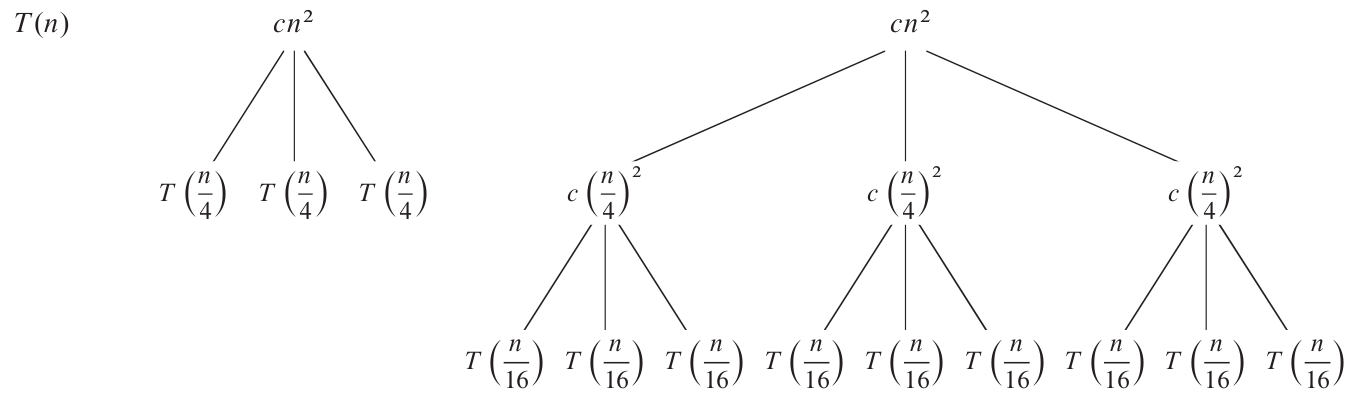
\includegraphics[width=1\textwidth]{figs/chap03/tree96-1}
\end{figure}
\end{itemize}
\end{frame}


\begin{frame}{‌روش درخت بازگشت}
\begin{itemize}\itemr
\item[-]
اگر مجموع هرینه‌ها را در هر سطح محاسبه کنیم، درختی با هزینه‌های قید شده در زیر خواهیم داشت.
\begin{figure}
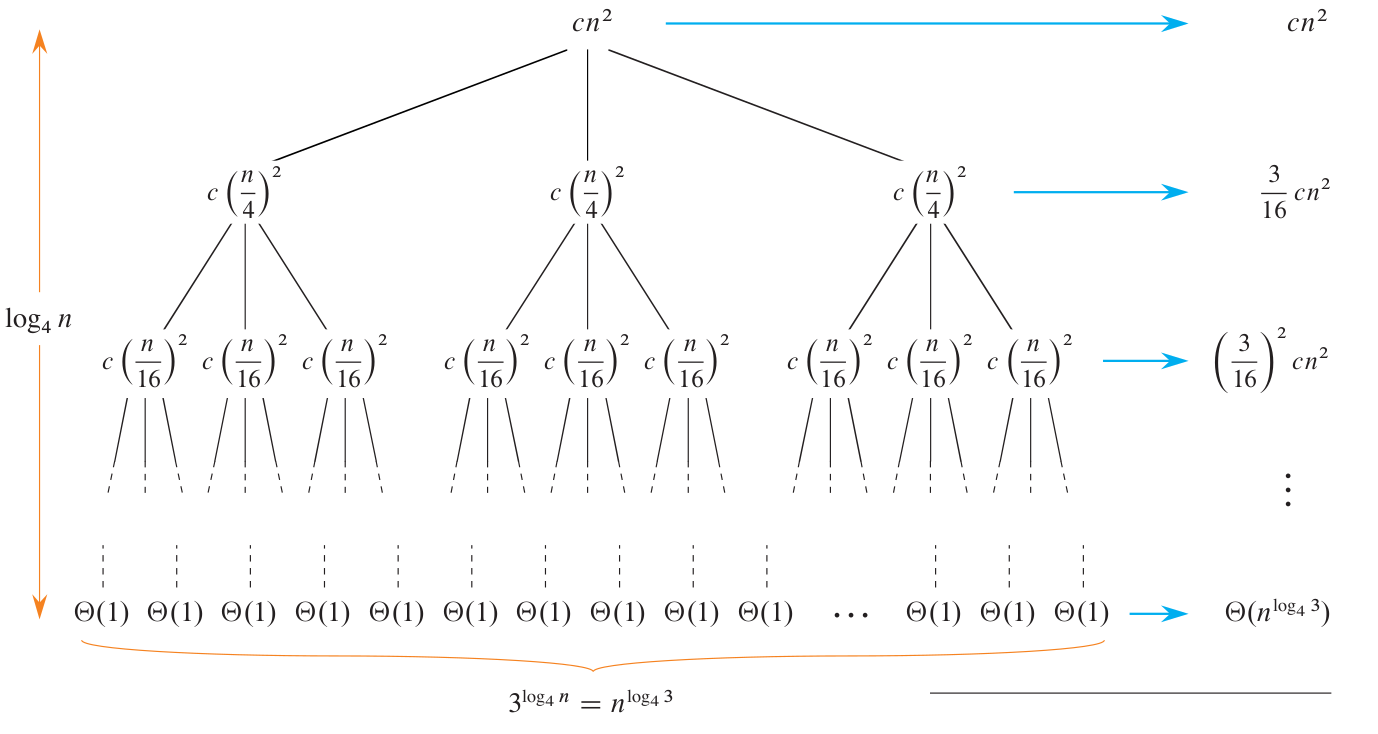
\includegraphics[width=0.9\textwidth]{figs/chap03/tree96-2}
\end{figure}
\end{itemize}
\end{frame}


\begin{frame}{‌روش درخت بازگشت}
\begin{itemize}\itemr
\item[-]
سپس هزینه‌های سطوح این درخت بازگشت را با هم جمع می‌کنیم و جواب رابطه بازگشتی را به دست می‌آوریم.
\end{itemize}
\end{frame}


\begin{frame}{‌روش درخت بازگشت}
\begin{itemize}\itemr
\item[-]
\begin{align*}
\m{T(n)} & \m{~= cn^2 + \frac{3}{16} cn^2 + {\left( \frac{3}{16} \right)}^2 cn^2 + \cdots +{\left( \frac{3}{16} \right)}^{\log_4 n} cn^2 + \ath {n^{\log_4 3}}}\\
& \m{~= {\sum_{i=0}^{\log_4 n}} {\left( \frac{3}{16} \right)}^i cn^2 + \ath {n^{\log_4 3}}} \\
& \m{~<  {\sum_{i=0}^{\infty}} {\left( \frac{3}{16} \right)}^i cn^2 + \ath {n^{\log_4 3}}}\\
& \m{~= \frac{1}{1 - (3/16)} cn^2 + \ath {n^{\log_4 3}}}\\
& \m{~= \frac{16}{13} cn^2 + \ath {n^{\log_4 3}}}\\
& \m{~= O(n^2)} ~~~~~~~~~~~~~~~~~~~~~~~~~~~~~~~~~~~ \m{(\ath {n^{\log_4 3}} = O(n^{0.8}) = O(n^2)).}
\end{align*}
\end{itemize}
\end{frame}


\begin{frame}{‌روش قضیه اصلی}
\begin{itemize}\itemr
\item[-]
روش قضیه اصلی
\fn{1}{master theorem method}
برای حل مسائل بازگشتی استفاده می‌شود که به صورت
\m{T(n) = aT(n/b) + f(n)}
هستند به طوری که
\m{a > 0}
و
\m{b > 1}
دو ثابت هستند.
\item[-]
تابع
\m{f(n)}
در اینجا تابع محرک
\fn{2}{driving function}
 نامیده می‌شود و یک رابطهٔ بازگشتی که به شکل مذکور است، رابطهٔ بازگشتی اصلی
\fn{3}{master recurrence}
  نامیده می‌شود.
\item[-]
در واقع رابطهٔ بازگشتی اصلی زمان اجرای الگوریتم‌های تقسیم و حل را توصیف می‌کند که مسئله‌ای به اندازهٔ n را به a زیر مسئله هر کدام با اندازهٔ
\m{n/b}
تقسیم می‌کنند. تابع
\m{f(n)}
هزینه تقسیم مسئله به زیر مسئله‌ها به علاوه هزینه ترکیب زیر مسئله‌ها را نشان می‌دهد.
\item[-]
اگر یک رابطهٔ بازگشتی شبیه رابطه قضیه اصلی باشد و علاوه بر آن چند عملگر کف و سقف در آن وجود داشته باشد، همچنان می‌توان از رابطهٔ قضیه اصلی استفاده کرد.
\end{itemize}
\end{frame}


\begin{frame}{‌روش قضیه اصلی}
\begin{itemize}\itemr
\item[-]
قضیه اصلی : فرض کنید
\m{a > 0}
و
\m{b > 1}
دو ثابت باشند و
\m{f(n)}
یک تابع باشد که برای اعداد بسیار بزرگ تعریف شده باشد.
\item[-]
رابطهٔ بازگشتی
\m{T(n)}
که بر روی اعداد طبیعی
\m{n \in \NN}
تعریف شده است را به صورت زیر در نظر بگیرید.
\begin{center}
\m{T(n) = aT(n/b) + f(n)}
\end{center}
\iffalse
به طوری که
\m{aT(n/b)}
برابر است با
\m{a'T( \lfloor n/b \rfloor ) + a"T(\lceil n/b \rceil)}
به ازای ثابت‌های
\m{a' \geqslant 0}
و
\m{a" \geqslant 0}
که در رابطهٔ
\m{a = a' + a"}
صدق می‌کنند.
\fi
\end{itemize}
\end{frame}


\begin{frame}{‌روش قضیه اصلی}
\begin{itemize}\itemr
\item[-]
 رفتار مجانبی
\m{T(n) = aT(n/b) + f(n)}
به صورت زیر است :
\item[۱-]
اگر ثابت
\m{\epsilon > 0}
وجود داشته باشد به طوری‌که
\m{f(n) = O(n^{\log_b^a - \epsilon})}
آنگاه
\m{T(n) = \ath{n^{\log_b^a}}}.
\item[۲-]
اگر ثابت
\m{k \geqslant 0}
وجود داشته باشد به طوری‌که
\m{f(n) = \ath{n^{\log_b^a} \lg^k n}}
آنگاه
\m{T(n) = \ath{n^{\log_b^a} \lg^{k+1}n}}.
\item[۳-]
اگر ثابت
\m{\epsilon > 0}
وجود داشته باشد به طوری‌که
\m{f(n) = \Omega(n^{\log_b^a + \epsilon})}
 آنگاه
\m{T(n) = \ath{f(n)}}.

برای برخی از توابع
\m{f(n)}
 نیاز داریم بررسی کنیم
\m{f(n)}
در رابطهٔ
\m{af(n/b) \leqslant cf(n)}
 به ازای
\m{c < 1}
و 
\m{n}
 های به اندازهٔ کافی بزرگ
صدق کند، اما برای توابعی که در تحلیل الگوریتم‌ها به آنها برمی‌خوریم این شرط معمولا برقرار است.
\end{itemize}
\end{frame}


\begin{frame}{‌روش قضیه اصلی}
\begin{itemize}\itemr
\item[۱-]
در حالت اول رشد جزء بازگشتی از رشد تابع محرک بیشتر است.
به عنوان مثال در
\m{T(n) = 2T(n/2) + \lg n}
رشد جزء بازگشتی
\ath{n}
و رشد تابع محرک
\ath{\lg n}
است.
بنابراین
\m{T(n) = \ath{n}} .
\item[۲-]
در حالت دوم رشد جزء بازگشتی و تابع محرک برابر است و یا رشد تابع محرک با یک ضریب
\ath{\lg^k n}
از جزء بازگشتی سریع‌تر است. به عنوان مثال در
\m{T(n) = 2T(n/2) + n \lg n}
رشد جزء بازگشتی
\ath{n}
و رشد تابع محرک
\ath{n \lg n}
است.
در این حالت تعداد سطوح درخت بازگشت 
\m{\lg n}
و مجموع هزینه‌های هر سطح
\ath{n \lg n}
است. بنابراین 
\m{T(n) = \ath{n \lg^2 n}} .
\item[۳-]
در حالت سوم رشد جزء بازگشتی از رشد تابع محرک کمتر است.
به عنوان مثال در
\m{T(n) = 2T(n/2) + n^2}
رشد جزء بازگشتی
\ath{n}
و رشد تابع محرک
\ath{n^2}
است.
بنابراین
\m{T(n) = \ath{n^2}} .
\end{itemize}
\end{frame}


\begin{frame}{‌روش قضیه اصلی}
\begin{itemize}\itemr
\item[-]
در یک حالت خاص اگر داشته باشیم، 
\m{T(n) = aT(n/b) + cn^k}
آنگاه می‌توانیم اثبات کنیم:
\begin{align*}
\m{T(n)} = \left\{\begin{array}{lr}
          \m{\Theta(n^{\log_b a})}& \m{a > b^k}~\text{اگر}\\
          \m{\Theta(n^k \lg n)}& \m{a = b^k}~\text{اگر}\\
          \m{\Theta(n^k)}& \m{a < b^k}~\text{اگر}
\end{array}\right.
\end{align*}

\end{itemize}
\end{frame}

\begin{frame}{‌روش قضیه اصلی}
\begin{itemize}\itemr
\item[-]
رابطهٔ بازگشتی
\m{T(n) = 9T(n/3) + n}
را در نظر بگیرید. در این رابطه داریم
\m{a = 9}
و
\m{b = 3}
بنابراین به دست می‌آوریم
\m{n^{\log_b^a} = n^{\log_3^9} = \ath{n^2}}.
از آنجایی که
\m{f(n) = n = O(n^{2- \epsilon})}
به ازای هر ثابت
\m{\epsilon < 1}
بنابراین می‌توانیم حالت اول در قضیه اصلی را در نظر بگیریم و نتیجه بگیریم
\m{T(n) = \ath{n^2}}.
\end{itemize}
\end{frame}


\begin{frame}{‌روش قضیه اصلی}
\begin{itemize}\itemr
\item[-]
رابطهٔ بازگشتی
\m{T(n) = T(2n/3) + 1}
را در نظر بگیرید. در این رابطه داریم
\m{a = 1}
و
\m{b = 3/2}
بنابراین
\m{n^{\log_b^a} = n^{\log_{3/2}^1} = n^0 = 1}.
در اینجا حالت دوم در قضیه اصلی را داریم یعنی
\m{f(n) = 1 = \ath{n^{\log_b^a} \lg^0 n} = \ath{1}}
بنابراین جواب رابطهٔ بازگشتی برابر است با
\m{T(n) = \ath{\lg n}}.
\end{itemize}
\end{frame}


\begin{frame}{‌روش قضیه اصلی}
\begin{itemize}\itemr
\item[-]
در رابطهٔ بازگشتی
\m{T(n) = 3T(n/4) + n\lg n}
داریم
\m{a = 3}
و
\m{b = 4}
که بدین معنی است که
\m{n^{\log_b^a} = n^{\log_4^3} = \ath{n^{0.793}}}.
از آنجایی که
\m{f(n) = n \lg n = \Omega (n^{\log_4^3 + \epsilon})}
جایی که
\m{\epsilon}
حدود
\m{0.2}
است، بنابراین حالت سوم در قضیه اصلی را می‌توانیم در نظر بگیریم اگر شرط
\m{af(n/b) \leqslant cf(n)}
برقرار باشد.
\begin{flushleft}
\m{af(n/b) = 3(n/4) \lg(n/4) \leqslant (3/4) n \lg n = 3/4f(n)}
\end{flushleft}
بنابراین با استفاده از حالت سوم جواب رابطهٔ بازگشتی برابراست با
\m{T(n) = \ath{n \lg n}}.
\end{itemize}
\end{frame}


\begin{frame}{‌روش قضیه اصلی}
\begin{itemize}\itemr
\item[-]
رابطهٔ بازگشتی
\m{T(n) = 2T(n/2) + \ath{n}}
رابطه‌ای بود که برای مرتب‌سازی ادغامی به دست آوردیم. از آنجایی که
\m{a = 2}
و
\m{b = 2}
داریم
\m{n^{\log_2^2} = n}.
حالت دوم در اینجا برقراراست زیرا به ازای
\m{k=0}
داریم
\m{f(n) = \ath{n}}
و بنابراین جواب رابطهٔ بازگشتی برابر است با
\m{T(n) = \ath{n \lg n}}.
\end{itemize}
\end{frame}


\begin{frame}{‌روش قضیه اصلی}
\begin{itemize}\itemr
\item[-]
رابطهٔ
\m{T(n) = 8T(n/2) + \ath{1}}
زمان اجرای الگوریتم ضرب ماتریسی را توصیف می‌کند. در اینجا داریم
\m{a = 8}
و
\m{b = 2}
بنابراین
\m{n^{\log_2^8} = n^3}.
تابع محرک
\m{f(n) = \ath{1}}
 است و بنابراین به ازای هر
\m{ \epsilon < 3}
داریم
\m{f(n) = O(n^{3 - \epsilon})} .
بنابراین حالت اول قضیه اصلی برقرار است. نتیجه می‌گیریم
\m{T(n) = \ath{n^3}}.
\end{itemize}
\end{frame}


\begin{frame}{‌روش قضیه اصلی}
\begin{itemize}\itemr
\item[-]
در تحلیل زمان اجرای الگوریتم استراسن رابطهٔ
\m{T(n) = 7T(n/2) + \ath{n^2}}
را به دست آوردیم. در این رابطهٔ بازگشتی
\m{a = 7}
و
\m{b = 2}
بنابراین
\m{n^{\log_2^7} = n^{\lg 7}}.
از آنجایی که
\m{\lg 7 = 2.8073...}
، می‌توانیم قرار دهیم
\m{\epsilon = 0.8}
و برای تابع محرک خواهیم داشت
\m{f(n) = \ath{n^2} = O \bigl( n^{\lg 7 - \epsilon} \bigr)}
، پس حالت اول در قضیه اصلی برقرار است و بنابراین جواب رابطهٔ بازگشتی برابر است با
\m{T(n) = \ath{n^{\lg 7}}}.
\end{itemize}
\end{frame}


\begin{itemframe}{مقدمه}
\itm
بسیاری از مسائل محاسباتی کاربردی ان‌پی کامل هستند و با این حال با توجه به اهمیت زیادی که دارند نیاز داریم جوابی برای آنها پیدا کنیم گرچه پیدا کردن جواب دقیق برای اینگونه مسائل در زمان چندجمله‌ای امکان‌پذیر نیست.
\itm
وقتی یک مسئله ان‌پی کامل است، برای حل آن سه راه پیش رو داریم : (۱) اگر ورودی نسبتاً کوچک باشد، می‌توان یک جواب بهینه در زمان نمایی به سرعت برای آن پیدا کرد. (۲) می‌توان یک حالت خاص از مسئله را در زمان چند جمله‌ای حل کرد. (۳) می‌توان یک جواب نزدیک به جواب بهینه در زمان چند جمله‌ای برای آن پیدا کرد. در بسیاری از کاربردها جواب نزدیک به جواب بهینه
\fn{near-optimal solution}
نیز کافی است. به چنین الگوریتم‌هایی که جواب نزدیک به بهینه تولید می‌کنند، الگوریتم‌های تقریبی
\fn{approximation algorithm}
می‌گوییم. برای بسیاری از مسائل ان‌پی کامل می‌توان یک الگوریتم تقریبی در زمان چندجمله‌ای پیدا کرد.
\end{itemframe}


\begin{itemframe}{مقدمه}
\itm
فرض کنید بر روی مسئلهٔ بهینه‌سازی کار می‌کنید که در آن هر یک از جواب‌های بالقوه
\fn{potential solution}
دارای یک هزینه است و می‌خواهید یک جواب نزدیک به بهینه پیدا کنید. بسته به نوع مسئله، ممکن است مسئله بیشینه سازی
\fn{maximization}
یا کمینه سازی
\fn{minimization}
باشد. می‌توانید یک جواب بهینه با هزینه حداکثر یا هزینه حداقل پیدا کنید.
\end{itemframe}

\begin{itemframe}{مقدمه}
\itm
می‌گوییم یک الگوریتم دارای «ضرب تقریب»
\fn{approximation ratio}
$\rho(n)$
است اگر به ازای هر ورودی با اندازهٔ n ، هزینهٔ
$C$
جواب تولید شده توسط الگوریتم نسبت به هزینهٔ
$C^*$
مربوط به جواب بهینه از مقدار
$\rho(n)$
کمتر باشد. به عبارت دیگر :
$$
\Bigl\{ \frac{C}{C^*}, \frac{C^*}{C} \Bigr\} \leqslant \rho(n)
$$
\itm
اگر یک الگوریتم دارای ضریب تقریب
$\rho(n)$
باشد، به آن الگوریتم تقریبی
$\rho(n)$
می‌گوییم.
\end{itemframe}


\begin{itemframe}{مقدمه}
\itm
از الگوریتم‌های تقریبی
$\rho(n)$
هم برای مسائل کمینه سازی و هم برای مسائل بیشینه سازی استفاده می‌شود.
\itm
در یک مسئله بیشینه سازی، داریم
$0 < C \leqslant C^*$
و بنابراین مقدار
$C^*/C$
مقدار بزرگ‌تری است که در آن هزینهٔ جواب بهینه از هزینهٔ جواب تقریبی بزرگ‌تر است.
\itm
در یک مسئله کمینه سازی، داریم
$0 < C^* \leqslant C$
و بنابراین مقدار
$C/C^*$
مقدار بزرگ‌تری است که در آن هزینهٔ جواب تقریبی از هزینهٔ جواب بهینه بزرگ‌تر است.
\itm
با فرض اینکه همهٔ هزینه‌ها مقادیر مثبت هستند، ضریب تقریب در یک الگوریتم تقریبی هیچ‌گاه کمتر از ۱ نیست.
\iffalse
 زیرا اگر داشته باشیم
$C/C^* \leqslant 1$
آنگاه
$C^*/C \geqslant 1$
.
\fi
\itm
بنابراین یک الگوریتم تقریبی با ضریب ۱ جوابی بهینه تولید می‌کند و هر چه ضریب تقریب الگوریتم تقریبی بیشتر باشد، جواب به دست آمده از جواب بهینه دورتر است.
\end{itemframe}


\begin{itemframe}{مقدمه}
\itm
برای بسیاری از مسائل، الگوریتم‌های تقریبی چند جمله‌ای با ضریب تقریب کوچک وجود دارد و برای برخی دیگر از مسائل، الگوریتم‌های تقریبی دارای ضریب تقریبی هستند که با مقدار n افزایش پیدا می‌کند.
\itm
در برخی از الگوریتم‌های تقریبی چندجمله‌ای، هرچه الگوریتم در زمان بیشتری اجرا شود، ضریب تقریب بهتری به دست می‌آید. در چنین مسائلی می‌توان با افزایش زمان محاسبات ضریب تقریب را بهبود داد.
\itm
این وضعیت حائز اهمّیت است و یک ناگذاری برای آن وجود دارد که در ادامه معرفی می‌کنیم.
\end{itemframe}

%todo this part is only usefull if an example of Approximation Scheme is mentioned delete it otherwise
\begin{itemframe}{مقدمه}
\itm
طرح تقریب
\fn{Approximation Scheme}
برای یک مسئلهٔ بهینه‌سازی، الگوریتمی تقریبی است که یک نمونه از مسئله را همراه با مقدار
$\varepsilon > 0$
دریافت می‌کند، به طوری که این الگوریتم یک الگوریتم تقریبی
$(1 + \varepsilon)$
 باشد.
\itm
اگر این طرح تقریب برای هر مقدار
$\epsilon > 0$
در زمانی چندجمله‌ای نسبت به اندازهٔ ورودی $n$ اجرا شود، آن را طرح تقریب چندجمله‌ای
\fn{Polynomial-Time Approximation Scheme}
 می‌نامیم.
\itm
زمان اجرای یک طرح تقریب چند جمله‌ایی ممکن است با کاهش
$\epsilon$
 به شدت افزایش یابد. برای مثال زمان اجرای آن می‌تواند چنین چیزی باشد:
$$
O(n^{2/\epsilon})
$$
\end{itemframe}


\begin{itemframe}{مقدمه}
\itm
اگر یک طرح تقریب، زمان اجرای چندجمله‌ای نسبت به هر دو پارامتر
$1/\varepsilon$
و $n$ داشته‌باشد، آن را «طرح تقریب چندجمله‌ای کامل»

\fn{Fully Polynomial-Time Approximation Scheme}
می‌نامیم. زمان اجرای یک طرح تقریب چند جمله‌ایی کامل می‌تواند چنین باشد:
$$
O((1/\epsilon)^2n^3)
$$
\itm
در چنین الگوریتمی، هر کاهش با ضریب ثابت در $\epsilon$، باعث افزایش زمان اجرا به‌اندازهٔ یک ضریب ثابت می‌شود.
\end{itemframe}

\begin{frame}{‌ضرب زنجیره‌ای ماتریس‌ها}
\begin{itemize}\itemr
\item[-]
مسئلهٔ ضرب زنجیره‌ای ماتریس‌ها
\fn{1}{Matrix-chain multiplication problem}
 به صورت زیر است. می‌خواهیم دنباله (زنجیره)ای از n ماتریس
\m{\langle A_1, A_2, \cdots, A_n \rangle}
را در هم ضرب کنیم. این ماتریس‌ها الزاماً ماتریس‌های مربعی نیستند و هدف این است که در این ضرب ماتریسی کمترین تعداد عملیات ضرب استفاده شود.
\item[-]
ضرب ماتریس‌ها شرکت پذیر
\fn{2}{associative}
، بدین معنی که پرانتز گذاری به هر نحوی انجام می‌شود، جواب ضرب ماتریسی تغییر نخواهد کرد.
\end{itemize}
\end{frame}


\begin{frame}{‌ضرب زنجیره‌ای ماتریس‌ها}
\begin{itemize}\itemr
\item[-]
الگوریتم ضرب دو ماتریس
\m{A(a_{ij})}
و
\m{B(b_{ij})}
به صورت زیر است. نتیجه ضرب این دو ماتریس در ماتریس
\m{C(c_{ij})}
ذخیره می‌شود.
\begin{algorithm}[H]\alglr
  \caption{Matrix Multiplication} 
  \begin{algorithmic}[1]
   \Func{Rectangular-Matrix-Multiply}{A, B, C, p, q, r}
     \For{i = 1 to p}
     	\For{j = 1 to r}
     		\For{k = 1 to q}
      			\State c[i,j] += a[i,k] * b[k,j]
     		\EndFor
     	\EndFor     		      			
     \EndFor                            
  \end{algorithmic}
  \label{alg:merge}
\end{algorithm}
\item[-]
برای اینکه ضرب ماتریسی درست باشد لازم است ابعاد ماتریس A برابر با
\m{p \times q}
و ابعاد ماتریس B برابر با
\m{q \times r}
باشد و ابعاد ماتریس حاصلضرب C در اینصورت برابر با
\m{p \times r}
خواهد بود. تعداد عملیات ضرب انجام شده برابر است با
\m{pqr}.
\end{itemize}
\end{frame}


\begin{frame}{‌ضرب زنجیره‌ای ماتریس‌ها}
\begin{itemize}\itemr
\item[-]
زنجیره ضرب ماتریسی
\m{A_1 \cdot A_2 \cdot A_3}
را در نظر بگیرید. فرض کنید ماتریس
\m{A_1}
با ابعاد
\m{10 \times 100}
، ماتریس
\m{A_2}
با ابعاد
\m{100 \times 5}
و ماتریس
\m{A_3}
با ابعاد
\m{5 \times 50}
باشد. اگر پرانتز گذاری به صورت
\m{((A_1A_2)A_3)}
باشد، تعداد
\m{10 \times 100 \times 5 = 5000}
عملیات ضرب برای ضرب
\m{A_1A_2}
و تعداد
\m{10 \times 5 \times 50 = 2500}
عملیات ضرب برای ضرب
\m{A_3}
در حاصلضرب
\m{A_1A_2}
باید انجام شود. بنابراین نیاز به انجام
\m{7500}
عملیات ضرب است.
\item[-]
حال فرض کنید پرانتز گذاری به صورت
\m{(A_1(A_2A_3))}
باشد. در اینصورت نیاز به انجام
\m{100 \times 5 \times 50 = 25000}
عملیات ضرب برای ضرب
\m{A_2A_3}
و نیاز به انجام 
\m{10 \times 100 \times 50 = 50000}
عملیات ضرب
برای ضرب
\m{A_1}
در حاصلضرب 
\m{A_2 A_3}
است،
بنابراین در مجموع نیاز به انجام
\m{75000}
عملیات ضرب است. بنابراین با استفاده از پرانتز گذاری اول، عملیات ضرب ۱۰ برابر سریع‌تر انجام می‌شود.
\end{itemize}
\end{frame}


\begin{frame}{‌ضرب زنجیره‌ای ماتریس‌ها}
\begin{itemize}\itemr
\item[-]
مسئله ضرب زنجیره‌ای ماتریس‌ها
را به صورت زیر بیان می‌کنیم :\\
زنجیرهٔ n ماتریس
\m{\langle A_1, A_2, \cdots, A_n \rangle}
را در نظر بگیرید، به طوری‌که به ازای
\m{i = 1,2, \cdots , n}
، ابعاد ماتریس
\m{A_i}
برابر است با
\m{p_{i-1} \times p_i}
. ضرب
\m{A_1 \cdot A_2 \cdots A_n}
را طوری پرانتز گذاری کنید که تعداد ضرب‌ها در عملیات ضرب این زنجیرهٔ ماتریسی حداقل باشد. ابعاد ورودی مسئله به صورت
\m{\langle p_0, p_1, p_2, \cdots, p_n \rangle}
داده شده‌اند.
\item[-]
در مسئله ضرب زنجیره‌ای ماتریس‌ها نمی‌خواهیم حاصلضرب ماتریس‌ها را به دست آوریم بلکه تنها می‌خواهیم ترتیب ضرب را به گونه‌ای به دست آوریم که هزینه ضرب به حداقل برسد. معمولا زمانی که صرف پیدا کردن پرانتز گذاری بهینه می‌شود ارزش هزینه کردن دارد، چرا که ممکن است ضرب ماتریس‌ها به صورت ترتیبی هزینهٔ گزافی به کاربر تحمیل کند.
\end{itemize}
\end{frame}


\begin{frame}{‌ضرب زنجیره‌ای ماتریس‌ها}
\begin{itemize}\itemr
\item[-]
قبل از اینکه این مسئله را حل کنیم، بررسی می‌کنیم چند پرانتز گذاری متفاوت وجود دارد. در واقع یک الگوریتم ساده برای حل این مسئله این است که هزینهٔ همهٔ پرانتز گذاری‌ها را با یکدیگر مقایسه کنیم ولی از آنجایی که تعداد پرانتز‌ گذاری‌ها بسیار زیاد است، بررسی همهٔ حالات مقدور نیست.
\item[-]
فرض کنید تعداد کل حالات برای پرانتز گذاری n ماتریس برابر باشد با
\m{P(n)}.
وقتی
\m{n = 1}
تنها یک ماتریس در زنجیره وجود دارد و بنابراین تنها یک حالت برای پرانتز گذاری وجود دارد. وقتی
\m{n \geqslant 2}
باشد، درواقع عبارت می‌تواند به دو قسمت شکسته شود به طوری‌که هر قسمت به طور جداگانه پرانتز گذاری شود. تعداد کل حالت‌های پرانتز گذاری برابر است با ضرب تعداد حالات پرانتز گذاری قسمت اول ضرب در تعداد حالت‌های پرانتز گذاری قسمت دوم.
\end{itemize}
\end{frame}


\begin{frame}{‌ضرب زنجیره‌ای ماتریس‌ها}
\begin{itemize}\itemr
\item[-]
این زنجیره می‌تواند به شکل‌های متعددی به دو قسمت تقسیم شود که با احتساب همهٔ حالت‌ها عبارت زیر را برای تعداد کل حالت‌های پرانتز گذاری به دست می‌آوریم.
\begin{align*}
\m{P(n)} = \left\{ \begin{array}{lr}
\m{1} & \m{n = 1}~~ \text{اگر}\\
\m{\sum_{k = 1}^{n - 1} P(k) P(n-k)} & \m{n \geqslant 2}~~ \text{اگر}
\end{array}\right.
\end{align*}
\item[-]
با حل این رابطهٔ بازگشتی به دست می‌آید
\m{P(n) = \Omega (2^n)}.
در واقع
\m{P(n)}
دنبالهٔ اعداد کاتالان
\fn{1}{catalan numbers}
(1, 1, 2, 5, 14, 42, 132, 429, 1430, 4862, 16796, 58786, ...)
را می‌سازد که رشد آن نمایی است و بنابراین به ازای n ‌های بسیار بزرگ، بررسی کردن همهٔ حالت‌ها در عمل غیرممکن است.
\end{itemize}
\end{frame}


\begin{frame}{‌ضرب زنجیره‌ای ماتریس‌ها}
\begin{itemize}\itemr
\item[-]
حال از روش برنامه‌ریزی پویا برای بهینه‌سازی پرانتز گذاری زنجیرهٔ ماتریسی استفاده می‌کنیم. یک الگوریتم به روش برنامه‌ریزی پویا برای یک مسئلهٔ بهینه‌سازی از چهار مرحله تشکیل شده است :
\item[۱-]
توصیف ساختار جواب بهینه بر اساس جواب بهینه زیرمسئله‌ها و بررسی اصل بهینگی
\item[۲-]
تعریف کردن مقدار جواب بهینه به طور بازگشتی
\item[۳-]
محاسبه کردن مقدار جواب بهینه
\item[۴-]
ساختن جواب بهینه توسط اطلاعات محاسبه شده
\end{itemize}
\end{frame}


\begin{frame}{‌ضرب زنجیره‌ای ماتریس‌ها}
\begin{itemize}\itemr
\item[-]
برای حل یک مسئلهٔ بهینه‌سازی توسط برنامه‌ریزی پویا باید مسئله دارای زیرساختار بهینه
\fn{1}{optimal substructure}
 باشد یا به عبارت دیگر اصل بهینگی
\fn{2}{principle of optimality}
  در آن برقرار باشد.
\item[-]
یک مسئله دارای زیرساختار بهینه است اگر جواب بهینه برای یک مسئله، شامل جواب‌های زیرمسئله‌ها باشد. به عبارت دیگر اگر جواب یک مسئلهٔ بهینه‌سازی را به دست آوریم، باید بتوانیم از جواب آن برای زیرمسئله‌ها نیز استفاده کنیم.
\item[-]
برای مثال مسئله کوتاهترین مسیر در گراف دارای زیرساختار بهینه است.
اگر کوتاهترین مسیر از x به y را به دست آوریم به طوری که مسیر از z عبور کند، کوتاهترین مسیر از x به z  و همچنین کوتاهترین مسیر از z به y نیز در جواب مسئله به دست آمده است.
\item[-]
اما مسئله بلندترین مسیر دارای زیرساختار بهینه نیست.
اگر بلندترین مسیر از x به y را به دست آوریم به طوری که مسیر از z عبور کند، نمی‌توانیم بگوییم بلندترین مسیر از z به y نیز در جواب مسئله است، زیرا ممکن است بلندترین مسیر از z به y از x عبور کند.
\end{itemize}
\end{frame}


\begin{frame}{‌ضرب زنجیره‌ای ماتریس‌ها}
\begin{itemize}\itemr
\item[-]
(گام ۱) توصیف ساختار جواب بهینه بر اساس جواب زیرمسئله‌ها و بررسی اصل بهینگی:
\item[-]
اولین مرحله در برنامه‌ریزی پویا تشخیص دادن ساختاری از مسئله است که در زیر مسئله‌ها نیز تکرار می‌شود. به عبارت دیگر اگر مسئله را برای یک زیر مسئله حل کنیم، باید بتوانیم با استفاده از اطلاعات زیر مسئله، مسئله را حل کنیم.
\item[-]
فرض کنید به ازای
\m{i \leqslant j}
ماتریس
\m{A_{i : j}}
از ضرب ماتریس‌های
\m{A_i A_{i+1} \cdots A_j}
به دست بیاید. اگر
\m{i = j}
باشد تنها یک پرانتز گذاری وجود دارد، اما اگر
\m{i < j}
باشد آنگاه برای پرانتز گذاری این عبارت می‌توانیم آن را به دو قسمت
\m{A_{i : k}}
و
\m{A_{k+1 : j}}
تقسیم کنیم به طوری‌که
\m{ i \leqslant k < j} .
با ضرب این دو ماتریس در یکدیگر، حاصل
\m{A_{i : j}}
را به دست می‌آوریم.
هزینهٔ پرانتز گذاری
\m{A_{i : j}}
برابر است با هزینه پرانتز گذاری
\m{A_{i : k}}
به علاوهٔ هزینهٔ پرانتز گذاری
\m{A_{k+1 : j}}
به علاوهٔ هزینهٔ ضرب دو قسمت در یکدیگر.
\end{itemize}
\end{frame}


\begin{frame}{‌ضرب زنجیره‌ای ماتریس‌ها}
\begin{itemize}\itemr
\item[-]
مسئلهٔ ضرب زنجیره‌ای ماتریس‌ها دارای زیرساختار بهینه است. به عبارت دیگر اگر یک پرانتزگذاری برای 
\m{A_{i:j}}
پیدا کنیم به طوری که به دو قسمت 
\m{A_{i:k}}
و
\m{A_{k+1:j}}
تقسیم شود، پرانتزگذاری
\m{A_{i:k}}
نیز بهینه است (به همین ترتیب پرانتزگذاری 
\m{A_{k+1:j}}
نیز بهینه است)
.
\item[-]
اثبات: فرض کنیم پرانتزگذاری 
\m{A_{i:j}}
 بهینه باشد و پرانتزگذاری
\m{A_{i:k}}
بهینه نباشد. در اینصورت می‌توانیم یک پرانتزگذاری بهینه برای 
\m{A_{i:k}}
پیدا کنیم و آن را در 
\m{A_{i:j}}
استفاده کنیم و یک پرانتزگذاری با هزینه کمتر برای 
\m{A_{i:j}}
به دست آوریم که با فرض اولیه در تناقض است. 
\end{itemize}
\end{frame}


\begin{frame}{‌ضرب زنجیره‌ای ماتریس‌ها}
\begin{itemize}\itemr
\item[-]
به طور خلاصه، اگر پرانتزگذاری بهینه برای
\m{A_{i : j}}
را پیدا کنیم، این پرانتزگذاری الزاما از دو پرانتزگذاری
\m{A_{i : k}}
و
\m{A_{k+1 : j}}
تشکیل شده است و الزاما پرانتزگذاری‌های
\m{A_{i : k}}
و
\m{A_{k+1 : j}}
نیز بهینه هستند.
\item[-]
بدین دلیل می‌توانیم از برنامه‌ریزی پویا استفاده کنیم، زیرا می‌توانیم هزینه‌های پرانتزگذاری‌های
\m{A_{i : k}}
و
\m{A_{k+1 : j}}
را از قبل ذخیره کنیم، و از این هزینه‌ها برای محاسبهٔ پرانتزگذاری
\m{A_{i : j}}
استفاده کنیم.
\end{itemize}
\end{frame}


\begin{frame}{‌ضرب زنجیره‌ای ماتریس‌ها}
\begin{itemize}\itemr
\item[-]
بنابراین باید مقدار 
\m{k}
 را پیدا کنیم به طوری‌که هزینهٔ پرانتز گذاری
\m{A_{i : k}}
به علاوهٔ هزینهٔ‌ پرانتزگذاری
\m{A_{k+1 : j}}
به علاوهٔ هزینهٔ ضرب
\m{A_{i : k}}
در
\m{A_{k+1 : j}}
بهینه باشد. آنگاه پرانتز گذاری
\m{A_{i : j}}
نیز بهینه خواهد بود.
\item[-]
پس برای حل مسئله یافتن هزینهٔ پرانتزگذاری بهینه برای
\m{A_{i : j}}
باید به ازای همهٔ 
\m{k}
 ها
هزینهٔ‌ پرانتزگذاری بهینه برای 
\m{A_{i : k}}
و 
\m{A_{k+1 : j}}
را محاسبه و با هزینهٔ ضرب
\m{A_{i : k}}
در
\m{A_{k+1 : j}}
جمع کنیم.
آنگاه از این میان 
\m{k}
 را به گونه‌ای انتخاب کنیم که هزینهٔ پرانتزگذاری 
بهینه باشد (تعداد ضرب‌های پرانتزگذاری
\m{A_{i : j}}
 کمترین مقدار ممکن باشد).
\iffalse
\item[-]
عبارت قبل را می‌توانیم به صورت زیر با استفاده از برهان خلف ثابت کنیم. فرض کنیم پرانتز گذاری
\m{A_{i : j}}
بهینه نباشد. این بدین معناست که یک پرانتز گذاری با هزینه کمتر وجود دارد. اما اگر یک پرانتز گذاری بهینه‌تر وجود داشته باشد می‌توان عبارت
\m{A_{i : j}}
را به دو قسمت تقسیم کرد و یک پرانتز گذاری بهتر برای
\m{A_{i : k}}
و
\m{A_{k+1 : j}}
پیدا کرد که در اینصورت به تناقض می‌رسیم.
\fi
\end{itemize}
\end{frame}



\begin{frame}{‌ضرب زنجیره‌ای ماتریس‌ها}
\begin{itemize}\itemr
\item[-]
(گام ۲) تعریف کردن مقدار جواب بهینه به طور بازگشتی :
\item[-]
فرض کنید
\m{m[i,j]}
حداقل تعداد ضرب‌های مورد نیاز برای محاسبه
\m{A_{i : j}}
باشد. حداقل تعداد ضرب‌های مورد نیاز برای کل n ماتریس یعنی
\m{A_{1 : n}}
برابراست با
\m{m[1,n]}.
\item[-]
می‌خواهیم یک عبارت بازگشتی برای مقدار
\m{m[i,j]}
محاسبه کنیم.
\item[-]
اگر
\m{i = j}
باشد، هزینه‌ای وجود ندارد، بنابراین
\m{m[i,j] = 0}.
\item[-]
اگر
\m{i < j}
باشد، از ساختار جواب بهینه برای زیر مسئله‌ها استفاده می‌کنیم. فرض کنید یک پرانتز گذاری بهینه حاصلضرب
\m{A_{i : j}}
را به دو قسمت
\m{A_{i : k}}
و
\m{A_{k+1 : j}}
تقسیم می‌کند به طوری‌که
\m{ i \leqslant k < j}.
بنابراین
\m{m[i,j]}
برابر است با هزینه
\m{m[i,k]}
برای محاسبه
\m{A_{i : k}}
به علاوه هزینه
\m{m[k+1,j]}
برای محاسبهٔ
\m{A_{k+1 : j}}
به علاوه هزینهٔ ضرب دو قسمت در یکدیگر. حاصلضرب
\m{A_{i : k} A_{k+1 : j}}
به تعداد
\m{p_{i-1} p_k p_j}
عملیات ضرب نیاز دارد. بنابراین داریم :
\begin{flushleft}
\m{m[i,j] = m[i,k] + m[k+1,j] + p_{i-1} p_k p_j}
\end{flushleft}
\end{itemize}
\end{frame}

\begin{frame}{‌ضرب زنجیره‌ای ماتریس‌ها}
\begin{itemize}\itemr
\item[-]
در رابطه قبل فرض کردیم مقدار k را می‌دانیم، اما از آنجایی که مقدار k ناشناخته است باید همهٔ مقادیر k به ازای
\m{k = i, i+1, \cdots , j-1}
امتحان کنیم تا مقدار بهینه
\m{m[i,j]}
را به‌دست آوریم. بنابراین رابطهٔ بازگشتی را در حالت کلی به صورت زیر می‌نویسیم.
\begin{align*}
\m{m[i,j]} = \left\{ \begin{array}{lr}
\m{0} & \m{i = j}~~ \text{اگر}\\
\m{min \{m[i,k] + m[k+1,j] + p_{i-1} p_k p_j : i \leqslant k < j} \} & \m{i < j}~~ \text{اگر}
\end{array}\right.
\end{align*}
\end{itemize}
\end{frame}


\begin{frame}{‌ضرب زنجیره‌ای ماتریس‌ها}
\begin{itemize}\itemr
\item[-]
(گام ۳) محاسبه کردن مقدار جواب بهینه:
\item[-]
حال می‌توانیم برنامه‌ای بنویسیم که به صورت بازگشتی رابطهٔ بازگشتی به دست آمده را محاسبه کند تا حداقل مقدار
\m{m[1,n]}
را به‌دست آوریم. این الگوریتم بازگشتی برای محاسبه، زمانی از مرتبه نمایی نیاز دارد، پس از این الگوریتم نیز در عمل برای n های بسیار بزرگ نمی‌توانیم استفاده کنیم.
\item[-]
مشکل الگوریتم بازگشتی این است که برخی از زیر مسئله‌ها یعنی برخی از
\m{m[i,j]}
‌ها ممکن است چندبار محاسبه شوند.
برای مثال برای دو پرانتزگذاری
\m{(A_{p:q})(A_{q+1})}
و
\m{(A_{p-1})(A_{p:q})}
دو بار باید هزینه پرانتزگذاری بهینه
\m{A_{p:q}}
محاسبه شود.
\item[-]
اما تعداد کل زیر مسئله‌ها به ازای
\m{1 \leqslant i \leqslant j \leqslant n}
برابراست با
\ath{n^2} .
%\begin{align*}
%\left( \begin{array}{c} \m{n} \\ \m{2} \end{array} \right) + \m{n} = \ath{n^2}
%\end{align*}
\iffalse
\item[-]
در واقع تعداد کل جفت‌های i و j هنگامی که برابر نباشند برابر است با 
\m{\binom{n}{2}} . 
اگر i و j برابر باشند، تعداد کل حالات برابر است با 
\m{n} .
\fi
\end{itemize}
\end{frame}


\begin{frame}{‌ضرب زنجیره‌ای ماتریس‌ها}
\begin{itemize}\itemr
\item[-]
به جای حل رابطه بازگشتی با استفاده از یک الگوریتم بازگشتی، آن را توسط جدولی حل می‌کنیم که مقادیر
\m{m[i,j]}
را از پایین به بالا محاسبه کند، بدین معنی که از
\m{m[1,1]}
شروع می‌کنیم و به ترتیب زیر مسئله‌های بزرگ‌تر را با استفاده از زیر مسئله‌های کوچکتر حل می‌کنیم.
\item[-]
به این روش حل مسئله
روش برنامه‌ریزی پویا گفته می‌شود.
در برنامه‌ریزی پویا مسئله به زیرمسأله‌ها شکسته شده، و حل مسئله با
 شروع از کوچکترین زیر مسئله‌ها آغاز می‌شود تا جواب مسئلهٔ اصلی با استفاده از زیر مسئله‌های کوچکتر محاسبه می‌شود.
\end{itemize}
\end{frame}


\begin{frame}{‌ضرب زنجیره‌ای ماتریس‌ها}
\begin{itemize}\itemr
\item[-]
الگوریتم زیر، مسئلهٔ بهینه‌سازی ضرب ماتریسی را به روش برنامه‌ریزی پویا حل می‌کند.
\end{itemize}
\end{frame}


\begin{frame}{‌ضرب زنجیره‌ای ماتریس‌ها}
\begin{algorithm}[H]\alglr
  \caption{Matrix Chain} 
  \begin{algorithmic}[1]
   \Func{Matrix-Chain-Order}{p , n}
     \State let m[1:n , 1:n] and s[1:n , 1:n] be new tables
     \For{i = 1 to n} \LeftComment{ chain length 1}
     	\State m[i,i] = 0 
     \EndFor
     \For{t = 2 to n} \LeftComment{t is the chain length}
        \For{i = 1 to n - t + 1}  \LeftComment{chain begins at Ai}
         \State j = i + t - 1 \LeftComment{chain ends at Aj}
         \State m[i,j] = $\infty$
         \For{k = i to j - 1} \LeftComment{try A[i:k] A[k+1 : j]}
         			\State q = m[i,k] + m[k+1,j] + p[i-1]*p[k]*p[j]
         			\If{q < m[i,j]}
         				\State m[i,j] = q \LeftComment{remember this cost}
         				\State s[i,j] = k  \LeftComment{remember this index}
         			\EndIf
         	\EndFor
         \EndFor
      \EndFor
  \State \Return m and s            
  \end{algorithmic}
  \label{alg:merge}
\end{algorithm}
\end{frame}


\begin{frame}{‌ضرب زنجیره‌ای ماتریس‌ها}
\begin{itemize}\itemr
\item[-]
زمان مورد نیاز برای حل این مسئله
\m{O(n^3)}
و حافظه مورد نیاز برای حل آن
\m{\ath{n^2}}
است، زیرا نیاز به نگهداری جدول برای محاسبه زیر مسئله‌ها می‌باشد.
\item[-]
با استفاده از برنامه‌ریزی پویا، زمان حل یک مسئله را از زمان نمایی به زمان چند جمله‌ای درجه سوم کاهش دادیم.
\end{itemize}
\end{frame}


\begin{frame}{‌ضرب زنجیره‌ای ماتریس‌ها}
\begin{itemize}\itemr
\item[-]
(گام ۴) ساختن جواب بهینه توسط اطلاعات محاسبه شده :
\item[-]
گرچه در گام قبل مقدار بهینه برای تعداد ضرب‌ها در یک زنجیرهٔ ماتریسی را محاسبه کردیم، اما روش پرانتزگذاری ماتریس‌ها را به دست نیاوردیم.
\item[-]
جدول
\m{s[1 : n , 1 : n]}
که در الگوریتم قبل محاسبه کردیم اطلاعات مورد نیاز برای جواب بهینه را نگهداری می‌کند. هر عنصر
\m{s[i , j]}
مقدار k را ذخیره می‌کند، به طوری که
\m{A_{i : j}}
به دو قسمت
\m{A_{i : k}}
و
\m{A_{k+1 : j}}
برای ضرب بهینه تقسیم می‌شود.
\end{itemize}
\end{frame}


\begin{frame}{‌ضرب زنجیره‌ای ماتریس‌ها}
\begin{itemize}\itemr
\item[-]
الگوریتم زیر پرانتز گذاری را برای مسئله ضرب زنجیرهٔ ماتریس‌ها انجام می‌دهد.
\begin{algorithm}[H]\alglr
  \caption{Print Optimal Parentheses} 
  \begin{algorithmic}[1]
   \Func{Print-Optimal-Parens}{s, i, j}
   \If{i == j}
   		\State print "A"i
   		\Else 
   		\State print "("
   		\State Print-Optimal-Parens (s, i, s[i, j])
   		\State Print-Optimal-Parens (s, s[i, j]+1, j)
   		\State print ")"
   	\EndIf
  \end{algorithmic}
  \label{alg:merge}
\end{algorithm}   
\end{itemize}
\end{frame}


\begin{frame}{‌ضرب زنجیره‌ای ماتریس‌ها}
\begin{itemize}\itemr
\item[-]
برای حل یک مسئله توسط روش برنامه‌ریزی پویا، مسئله باید دو ویژگی داشته باشد.
\item[-]
ویژگی اول این است که مسئله را باید بتوان با استفاده از جواب زیر مسئله‌های آن به دست آورد. درواقع باید بتوان برای مسئله زیر مسئله‌هایی پیدا کرد که ساختار آنها شبیه مسئله اصلی است.
به عبارت دیگر مسئله باید دارای زیرساختار بهینه باشد.
\item[-]
 ویژگی دوم این است که اگر بخواهیم مسئله را توسط الگوریتم بازگشتی حل کنیم باید زیر مسئله‌ها همپوشانی داشته باشند. بدین ترتیب جدول برنامه‌ریزی پویا راه‌حلی برای جلوگیری از محاسبات تکراری در این همپوشانی‌ها خواهد بود.
\end{itemize}
\end{frame}

\begin{frame}{‌طولانی‌ترین زیر رشته مشترک}
\begin{itemize}\itemr
\item[-]
برخی مواقع زیست شناسان نیاز دارند دو یا چند ارگانیسم مختلف را با یکدیگر مقایسه کنند. برای این کار دی‌ان‌ای این ارگانیسم‌ها باید مقایسه شوند. یک رشتهٔ دی‌ان‌ای شامل رشته‌ای از مولکول‌ها به نام مولکول‌های پایه است که می‌توانند آدنین
\fn{1}{adenine}
، سیتوزین
\fn{2}{cytosine}
، گرانین
\fn{3}{granine}
، یا تیمین
\fn{4}{thymine}
باشند. هریک از این مولکول‌های پایه با یک حرف نشان داده می‌شوند، بنابراین یک رشته دی‌ان‌ای، یک رشته بر روی الفبای
\m{\{A, C, G, T \}}
است. برای مثال
\m{S_1 = ACCGGTC}
یک رشته دی‌ان‌ای است.
\item[-]
یکی از دلایلی که نیاز داریم دو رشتهٔ دی‌ان‌ای را با یکدیگر مقایسه کنیم، برای این است که متوجه شویم دو ارگانیسم چقدر به یکدیگر شباهت دارند.
\end{itemize}
\end{frame}


\begin{frame}{‌طولانی‌ترین زیر رشته مشترک}
\begin{itemize}\itemr
\item[-]
روش‌های مختلفی برای سنجش شباهت دو رشتهٔ دی‌ان‌ای وجود دارند.
%یک روش برای سنجش شباهت دو رشتهٔ دی‌ان‌ای این است که برای شباهت یک مقدار عددی تعریف کنیم. این مقدار عددی برابر است با تعداد تغییرات مورد نیاز در یک رشته برای به دست آوردن رشتهٔ دیگر.
\item[-]
یک روش برای سنجش شباهت این است که زیر رشته‌های مشترک بین دو رشته را پیدا کنیم. هرچقدر این زیر رشته‌های مشترک طول بیشتری داشته باشند، دو رشته به یکدیگر شبیه‌ترند.
\item[-]
در این روش برای مقایسه دو رشته باید زیر رشته‌های مشترک محاسبه شوند و طولانی‌ترین آنها پیدا شود. به این مسئله، مسئلهٔ پیدا کردن طولانی‌ترین زیر رشته مشترک
\fn{1}{longest common subsequence}
گفته می‌شود.
\end{itemize}
\end{frame}


\begin{frame}{‌طولانی‌ترین زیر رشته مشترک}
\begin{itemize}\itemr
\item[-]
یک زیر دنباله از یک دنباله، دنباله‌ای است که از حذف صفر یا بیشتر عنصر از دنباله اصلی به دست بیاید.
\item[-]
به طور رسمی، به ازای دنبالهٔ
\m{X = \langle x_1, x_2, \cdots , x_m \rangle}
، دنبالهٔ
\m{Z = \langle z_1, z_2, \cdots , z_k \rangle}
را زیر دنباله
\fn{1}{subsequence}
\m{X}
می‌نامیم اگر دنبالهٔ صعودی
\m{\langle i_1, i_2, \cdots , i_k \rangle}
از اندیس‌های
\m{X}
وجود داشته باشند، به طوری‌که به ازای
\m{j = 1,2, \cdots , k}
داشته باشیم
\m{x_{i_j} = z_j}.
\item[-]
 برای مثال دنبالهٔ
\m{Z = \langle B,C,D,B \rangle}
 یک زیردنباله از دنبالهٔ
\m{X = \langle A,B,C,B,D,A,B \rangle}
 است با اندیس‌های
\m{\langle 2,3,5,7 \rangle} .
\end{itemize}
\end{frame}


\begin{frame}{‌طولانی‌ترین زیر رشته مشترک}
\begin{itemize}\itemr
\item[-]
به ازای دو دنبالهٔ
\m{X}
و
\m{Y}
، می‌گوییم دنبالهٔ
\m{Z}
یک زیردنبالهٔ مشترک
\fn{1}{common subsequence}
\m{X}
و
\m{Y}
است اگر
\m{Z}
زیر دنباله‌ای از
\m{X}
و همچنین
\m{Y}
باشد.
\item[-]
برای مثال اگر
\m{X = \langle A,B,C,B,D,A,B \rangle}
و
\m{Y = \langle B,D,C,A,B,A \rangle}
باشند آنگاه
\m{\langle B,C,A \rangle}
یک زیردنبالهٔ مشترک
\m{X}
و
\m{Y}
است.
\item[-]
دنبالهٔ
\m{\langle B,C,A \rangle}
با طول ۳ طولانی‌ترین زیر دنبالهٔ مشترک
\m{X}
و
\m{Y}
نیست، چرا که دنبالهٔ
\m{\langle B,C,B,A \rangle}
با طول ۴ وجود دارد که زیر دنبالهٔ مشترک
\m{X}
و
\m{Y}
است. این زیردنباله، طولانی‌ترین زیر دنبالهٔ مشترک
\fn{2}{longest common subsequence}
\m{X}
و
\m{Y}
است، چرا که زیردنبالهٔ مشترک بلندتری وجود ندارد.
\end{itemize}
\end{frame}



\begin{frame}{‌طولانی‌ترین زیر رشته مشترک}
\begin{itemize}\itemr
\item[-]
می‌توانیم مسئله طولانی‌ترین زیردنبالهٔ مشترک را با استفاده از یک روش جستجوی کامل
\fn{1}{exhaustive search (brute-force search)}
به دست آوریم، بدین معنی که همهٔ زیردنباله‌های مشترک دو رشته را به دست آوریم و مقایسه کنیم. از آنجایی که رشته
\m{X}
با طول m تعداد
\m{2^m}
زیردنباله دارد، بنابراین این روش برای رشته‌های طولانی غیر قابل استفاده است.
\item[-]
می‌خواهیم این مسئله را به روش برنامه‌ریزی پویا حل کنیم.
\end{itemize}
\end{frame}



\begin{frame}{‌طولانی‌ترین زیر رشته مشترک}
\begin{itemize}\itemr
\item[-]
گام اول : مشخص کردن ساختار جواب مسئله بر اساس زیرمسئله‌ها
\item[-]
برای تعریف مسئله طولانی‌ترین زیررشتهٔ مشترک با استفاده از زیر مسئله‌ها، ابتدا مفهوم پیشوند
\fn{1}{prefix}
یک دنباله را تعریف می‌کنیم.
\item[-]
به ازای دنبالهٔ
\m{X = \langle x_1, x_2, \cdots , x_m \rangle}،
i
امین پیشوند
\m{X}
برابراست با
\m{X_i = \langle x_1, x_2, \cdots , x_i \rangle}
به ازای
\m{i = 0,1, \cdots , m}.
\item[-]
برای مثال اگر
\m{X = \langle A,B,C,B,D,A,B \rangle}
باشد، آنگاه
\m{X_4 = \langle A,B,C,B \rangle}
و
\m{X_0}
دنبالهٔ تهی است.
\end{itemize}
\end{frame}


\begin{frame}{‌طولانی‌ترین زیر رشته مشترک}
\begin{itemize}\itemr
\item[-]
فرض کنید
\m{X = \langle x_1, x_2, \cdots , x_m \rangle}
و
\m{Y = \langle y_1, y_2, \cdots , y_n \rangle}
دو دنباله باشند و
\m{Z = \langle z_1, z_2, \cdots , z_k \rangle}
طولانی‌ترین زیررشته مشترک
\m{X}
و
\m{Y}
باشد. خواهیم داشت :
\item[۱-]
اگر
\m{x_m = y_n}
آنگاه
\m{z_k = x_m = y_n}
و
\m{Z_{k-1}}
طولانی‌ترین زیر رشته مشترک
\m{X_{m-1}}
و
\m{Y_{n-1}}
است.
\item[۲-]
اگر
\m{x_m \neq y_n}
و
\m{z_k \neq x_m}
باشد، آنگاه
\m{Z}
طولانی‌ترین زیر رشته مشترک
\m{X_{m-1}}
و
\m{Y}
است.
\item[۳-]
اگر
\m{x_m \neq y_n}
و
\m{z_k \neq y_n}
باشد، آنگاه
\m{Z}
طولانی‌ترین زیر رشته مشترک
\m{X}
و
\m{Y_{n-1}}
است.
\end{itemize}
\end{frame}


\begin{frame}{‌طولانی‌ترین زیر رشته مشترک}
\begin{itemize}\itemr
\item[-]
گزاره‌های ۱، ۲ ، ۳ در قضیه قبل را به ترتیب اثبات می‌کنیم.
\item[۱-]
اگر
\m{x_m = y_n}
آنگاه
\m{z_k = x_m = y_n}
و
\m{Z_{k-1}}
طولانی‌ترین زیر رشته مشترک
\m{X_{m-1}}
و
\m{Y_{n-1}}
است.
\\~
\\~
اثبات: اگر
\m{x_m = y_n}
باشد، الزاما باید داشته باشیم
\m{z_k = x_m}.
این گزاره را با برهان خلف ثابت می‌کنیم. فرض کنید
\m{z_k \neq x_m}
، آنگاه می توانیم
\m{x_m}
که برابر با
\m{y_n}
است را به
\m{Z}
بیافزاییم و زیررشته مشترکی پیدا کنیم که طول آن
\m{k+1}
است. از آنجایی که در صورت مسئله گفته شده
\m{Z}
طولانی‌ترین زیر رشته مشترک با طول
\m{k}
است، پس به تناقض می‌رسیم. پس فرض اولیه نادرست است و الزاما باید داشته باشیم
\m{z_k = x_m = y_n}.
\iffalse
پس
\m{Z_{k-1}}
یعنی
\m{k-1}
امین پیشوند
\m{Z}
باید یک زیررشته مشترک
\m{X_{m-1}}
و
\m{Y_{n-1}}
باشد.
\fi
حال باید ثابت کنیم
\m{Z_{k-1}}
طولانی‌ترین زیر رشته مشترک
\m{X_{m-1}}
و
\m{Y_{n-1}}
نیز هست. این گزاره را با برهان خلف ثابت می‌کنیم. فرض یک زیر رشته مشترک
\m{W}
برای
\m{X_{m-1}}
و
\m{Y_{n-1}}
وجود دارد که طول آن از
\m{k-1}
بیشتر است. در اینصورت با اضافه کردن
\m{x_m = y_n}
به
\m{W}
زیر رشته‌ای ساخته می‌شود که طول آن از
\m{k}
بیشتر است. اما در اینجا به تناقض می‌رسیم چون فرض کردیم طول بلندترین زیر رشته مشترک
\m{k}
است.
\end{itemize}
\end{frame}


\begin{frame}{‌طولانی‌ترین زیر رشته مشترک}
\begin{itemize}\itemr
\item[۲-]
اگر
\m{x_m \neq y_n}
و
\m{z_k \neq x_m}
باشد، آنگاه
\m{Z}
طولانی‌ترین زیر رشته مشترک
\m{X_{m-1}}
و
\m{Y}
است.
\\~
\\~
اثبات: اگر
\m{z_k \neq x_m}
باشد، آنگاه
\m{Z}
یک زیر رشته مشترک برای
\m{X_{m-1}}
و
\m{Y}
است. اگر یک زیر رشته مشترک دیگر به نام
\m{W}
با طول بیشتر از
\m{k}
برای
\m{X_{m-1}}
و
\m{Y}
وجود داشت، آنگاه
\m{W}
می‌توانست یک زیر رشته مشترک برای
\m{X}
و
\m{Y}
نیز باشد که این متناقض است با فرض اینکه
\m{Z}
بلندترین زیر رشته مشترک
\m{X}
و
\m{Y}
با طول
\m{k}
است.
\item[۳-]
اگر
\m{x_m \neq y_n}
و
\m{z_k \neq y_n}
باشد، آنگاه
\m{Z}
طولانی‌ترین زیر رشته مشترک
\m{X}
و
\m{Y_{n-1}}
است.
\\~
\\~
اثبات: شبیه و متقارن حالت ۲ است.
\end{itemize}
\end{frame}


\begin{frame}{‌طولانی‌ترین زیر رشته مشترک}
\begin{itemize}\itemr
\item[-]
بنابراین توانستیم مسئله طولانی‌ترین زیر رشته مشترک را بر اساس زیر مسئله‌های بهینه آن تعریف کنیم. جواب زیر مسئله‌های در همهٔ حالت‌های بررسی شده در جواب مسئله وجود دارد.
\item[-]
پس این مسئله دارای زیرساختار بهینه است.
\end{itemize}
\end{frame}



\begin{frame}{‌طولانی‌ترین زیر رشته مشترک}
\begin{itemize}\itemr
\item[-]
گام دوم : تعریف کردن مقدار جواب به صورت بازگشتی
\item[-]
فرض کنید 
\m{c[i,j]}
طول بلندترین زیررشتهٔ مشترک 
\m{X_i}
و
\m{Y_j}
باشد.
\item[-]
 این مسئله بهینه‌سازی را می‌توانیم بر اساس زیر ساختارهای بهینه به صورت زیر تعریف کنیم.
\begin{align*}
\m{c[i,j]} = \left\{\begin{array}{lr}
          \m{0}& \m{j = 0}~\text{یا}~\m{i = 0}~\text{اگر}\\
          \m{c[i-1,j-1] + 1}& \m{x_i = y_j}~\text{و}~\m{i,j > 0}~\text{اگر}\\
          \m{\max \{c[i,j-1],c[i-1,j] \}}& \m{x_i \neq y_j}~\text{و}~\m{i,j > 0}~\text{اگر}
\end{array}\right.
\end{align*}
\item[-]
دقت کنید که اگر الگوریتم بازگشتی برای حل این مسئله استفاده شود زیر مسئله‌ها به طور تکراری محاسبه می‌شوند. پس می‌توانیم در این‌جا از برنامه‌ریزی پویا استفاده کنیم.
\end{itemize}
\end{frame}



\begin{frame}{‌طولانی‌ترین زیر رشته مشترک}
\begin{itemize}\itemr
\item[-]
گام سوم : محاسبه طول طولانی‌ترین زیر دنباله مشترک
\item[-]
از آنجایی که برای دو دنباله
\m{X = \langle x_1, x_2, \cdots , x_m \rangle}
و
\m{Y = \langle y_1, y_2, \cdots , y_n \rangle}
مقادیر جدول
\m{c[0:m,0:n]}
باید محاسبه شوند و هر خانه از جدول در زمان ثابت
\ath{1}
محاسبه می‌شود، بنابراین زمان اجرای الگوریتم برنامه‌ریزی پویا برای این مسئله برابراست با
\ath{mn}
. طول زیر رشته مشترک برابراست با مقدار محاسبه شده برای
\m{c[m,n]}.
\end{itemize}
\end{frame}


\begin{frame}{‌طولانی‌ترین زیر رشته مشترک}
\begin{itemize}\itemr
\item[-]
الگوریتم طولانی‌ترین زیررشته مشترک به صورت زیر نوشته شده است.
\begin{algorithm}[H]\alglr
  \caption{Longest Common Subsequence Length} 
  \begin{algorithmic}[1]
   \Func{LCS-Length}{X,Y, m, n} 
    \State let b[1:m, 1:n] and c[0:m, 0:n] be new tables
    	\For{i = 1 \To m} 
      		\State c[i,0] = 0
       \EndFor
    	\For{j = 0 \To n} 
      		\State c[0,j] = 0
       \EndFor                                       
  \end{algorithmic}
  \label{alg:merge}
\end{algorithm}
\end{itemize}
\end{frame}


\begin{frame}{‌طولانی‌ترین زیر رشته مشترک}
\begin{itemize}\itemr
\item[-]
\begin{algorithm}[H]\alglr
  \caption{Longest Common Subsequence Length} 
  \begin{algorithmic}[1]
   \setcounter{ALG@line}{5}
   \Func{LCS-Length}{X,Y, m, n} 
    	\For{i = 1 \To m} \LeftComment{compute table entries in row-major order} 
        	\For{j = 1 \To n}
        		\If{X[i] == Y[j]}
        			\State c[i, j] = c[i-1, j-1] + 1
        			\State b[i, j] = "$\nwarrow$"
        		\ElsIf{c[i-1, j] $\geqslant$ c[i, j-1]}
        			\State c[i, j] = c[i-1, j] 
        			\State b[i, j] = "$\uparrow$"
        		\Else
        		    \State c[i, j] = c[i, j-1]
        			\State b[i, j] = "$\leftarrow$"
        		\EndIf
        	\EndFor
        \EndFor
    \State \Return c and b	                                         
  \end{algorithmic}
  \label{alg:merge}
\end{algorithm}
\end{itemize}
\end{frame}


\begin{frame}{‌طولانی‌ترین زیر رشته مشترک}
\begin{itemize}\itemr
\item[-]
گام چهارم : ساختن بلندترین زیر دنبالهٔ مشترک
\item[-]
با استفاده از جدول b که توسط الگوریتم قبل ساخته شده می‌توانیم زیر دنبالهٔ مشترک
\m{X}
و
\m{Y}
را بسازیم، بدین ترتیب که با
\m{b[m,n]}
شروع می‌کنیم و جهت نشانه‌ها را دنبال می‌کنیم. علامت
\m{\nwarrow}
در جدول b نشان می‌دهد که
\m{x_i = y_j}
در طولانی‌ترین زیررشتهٔ مشترک است.
\end{itemize}
\end{frame}


\begin{frame}{‌طولانی‌ترین زیر رشته مشترک}
\begin{itemize}\itemr
\item[-]
برای مثال به ازای دو دنبالهٔ
\m{X = \langle A,B,C,B,D,A,B \rangle}
و
\m{Y = \langle B,D,C,A,B,A \rangle}
جدول زیر به‌دست می‌آید.
\begin{figure}
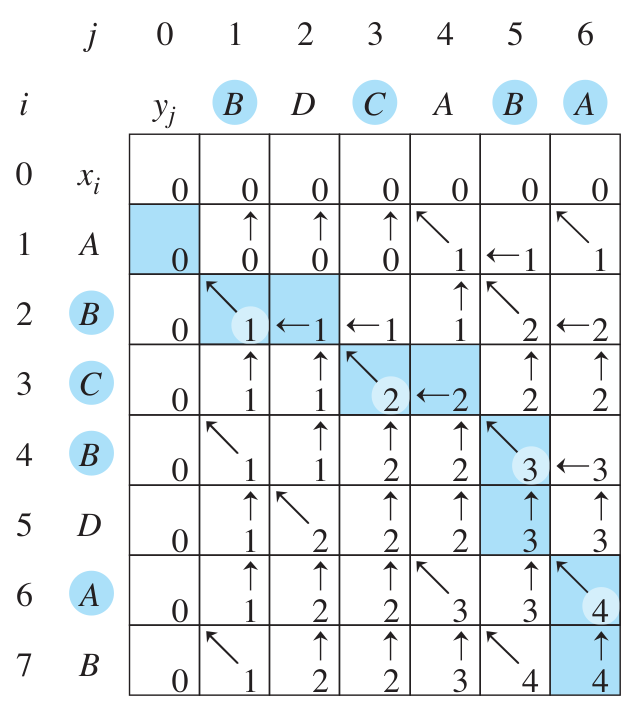
\includegraphics[width=0.4\textwidth]{figs/chap04/lcs-example}
\end{figure}
\end{itemize}
\end{frame}


\begin{frame}{‌طولانی‌ترین زیر رشته مشترک}
\begin{itemize}\itemr
\item[-]
\begin{algorithm}[H]\alglr
  \caption{Print Longest Common Subsequence} 
  \begin{algorithmic}[1]
   \Func{Print-LCS}{b, X, i, j}
		\If{i == 0 or j ==0}
				\State \Return \LeftComment{the longest common subsequence has length 0}
		\EndIf
		\If{b[i, j] == "$\nwarrow$"}
			\State Print-LCS(b, X, i-1, j-1)
			\State print X[i] \LeftComment{same as Y[j]}
		\ElsIf{b[i, j] = "$\uparrow$"}
			\State Print-LCS(b, X, i-1, j)
		\Else{\State Print-LCS(b, X, i, j-1)}
		\EndIf
  \end{algorithmic}
  \label{alg:merge}
\end{algorithm}  
\end{itemize}
\end{frame}




\begin{frame}{‌طولانی‌ترین زیر رشته مشترک}
\begin{itemize}\itemr
\item[-]
پس از طراحی یک الگوریتم معمولاً به دنبال روش‌هایی برای بهبود در زمان اجرا و میزان حافظه می‌گردیم.
\item[-]
در الگوریتم طولانی‌ترین زیر دنبالهٔ مشترک به طور مثال می توانیم جدول b را حذف کنیم و اطلاعات لازم برای ساختن بلندترین زیر دنبالهٔ مشترک را از جدول c به دست آوریم.
\item[-]
هریک از درایه‌های
\m{c[i,j]}
از طریق یکی از سه درایهٔ
\m{c[i-1,j-1]}
،
\m{c[i-1,j]}
،
\m{c[i,j-1]}
محاسبه شده است که در زمان ثابت می‌توانیم بدون جدول b به دست آوریم درایه
\m{c[i,j]}
چگونه محاسبه شده است.
\item[-]
بنابراین طولانی‌ترین زیردنبالهٔ مشترک را می‌توانیم همچنان در زمان
\ath{m+n}
بسازیم و جدول b را حذف کرده و از حافظهٔ مورد نیاز به میزان
mn
بکاهیم.
\end{itemize}
\end{frame}

\begin{frame}{‌درخت جستجوی دودویی بهینه}
\begin{itemize}\itemr
\item[-]
فرض کنید می‌خواهیم برنامه‌ای طراحی کنیم که متون انگلیسی را به فارسی ترجمه کند. به ازای هر کلمهٔ انگلیسی در یک متن باید با استفاده از یک فرهنگ لغت، معادل فارسی آن را بیابیم. برای یک جستجوی بهینه می‌توانیم یک درخت جستجوی دودویی با n رأس بسازیم که هر رأس آن یک کلمهٔ انگلیسی و معادل فارسی آن را شامل شود.
\item[-]
اگر از یک درخت جستجوی دودویی متوازن
\fn{1}{balanced binary search tree}
%مانند درخت قرمز-سیاه
%\fn{2}{red-black tree}
استفاده کنیم، می‌توانیم جستجوی هر کلمه را در یک درخت با n کلمه در زمان
\m{O(\lg n)}
انجام دهیم.
\end{itemize}
\end{frame}

\begin{frame}{‌درخت جستجوی دودویی بهینه}
\begin{itemize}\itemr
\item[-]
اما کلمات مختلف تعداد تکرارهای مختلف دارند. برای مثال کلمات a یا the در انگلیسی بسیار پر تکرارند و بهتر است این کلمات در درخت جستجو به ریشه نزدیک‌تر باشند و برخی از اسامی خاص بسیار کم تکرارند و بهتر است که فاصلهٔ آنها از ریشه بیشتر باشد.
\item[-]
با استفاده از درخت جستجوی دودویی بهینه
\fn{1}{optimal binary search tree}
می‌توان کلمات را به گونه‌ای ذخیره و بازیابی کرد که کلمات با احتمال وقوع بیشتر نزدیک‌تر به ریشه قرار بگیرند.
\end{itemize}
\end{frame}


\begin{frame}{‌درخت جستجوی دودویی بهینه}
\begin{itemize}\itemr
\item[-]
دنبالهٔ
\m{K = \langle k_1, k_2, \cdots , k_n \rangle}
با n کلید را در نظر بگیرید به طوری‌که
\m{k_1 < k_2 < \cdots < k_n} .
\item[-]
می‌خواهیم یک درخت جستجوی دودویی بهینه حاوی این کلیدها بسازیم.
\item[-]
به ازای هر یک از کلیدهای
\m{k_i}
، یک احتمال وقوع
\m{p_i}
نیز داده شده است.
\item[-]
از آنجایی که برخی از کلیدها در درخت جستجو وجود ندارد‌ (برای مثال کلماتی در کاربرد ترجمه در انگلیسی وجود دارند که معادل فارسی ندارند) ، تعداد
\m{n+1}
کلید بی‌استفاده
\m{d_0, d_1, d_2, \cdots, d_n}
نیز داریم که نماینده این کلیدها هستند. در واقع
\m{d_0}
نمایندهٔ همهٔ کلیدهایی است که از
\m{k_1}
کوچکترند و
\m{d_n}
نمایندهٔ همهٔ کلیدهایی است که از
\m{k_n}
بزرگ‌ترند و همچنین به ازای
\m{i = 1,2, \cdots, n-1}
، کلید
\m{d_i}
نمایندهٔ همهٔ مقادیری است که بین
\m{k_i}
و
\m{k_{i+1}}
قرار دارند. همچنین به ازای هر کلید
\m{d_i}
یک احتمال وقوع
\m{q_i}
داریم.
\end{itemize}
\end{frame}


\begin{frame}{‌درخت جستجوی دودویی بهینه}
\begin{itemize}\itemr
\item[-]
در شکل زیر دو درخت جستجوی دودویی بهینه را با تعداد ۵ کلید مشاهده می‌کنیم.
\begin{figure}
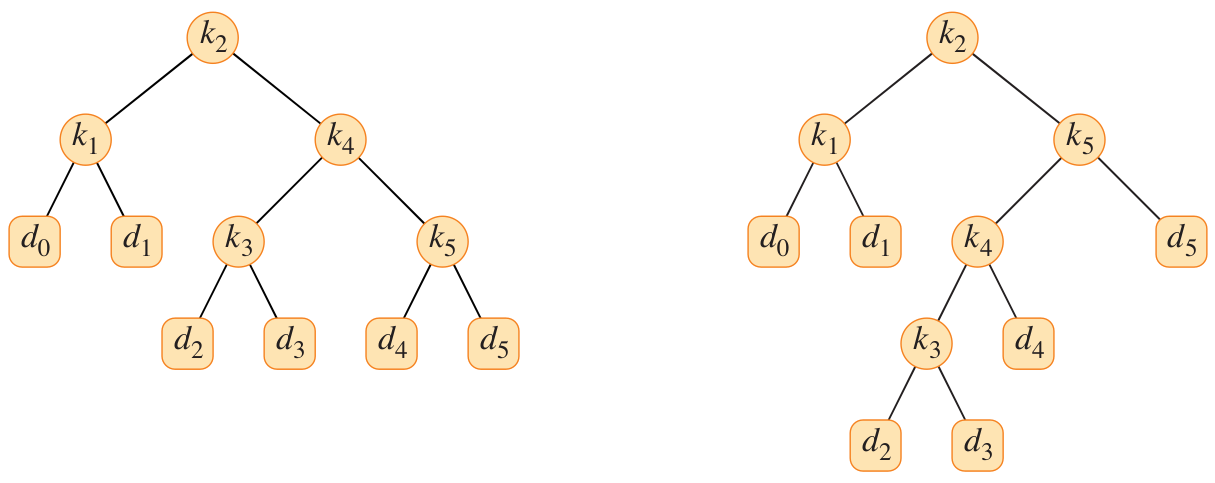
\includegraphics[width=0.9\textwidth]{figs/chap04/optimal-tree}
\end{figure}
\end{itemize}
\end{frame}


\begin{frame}{‌درخت جستجوی دودویی بهینه}
\begin{itemize}\itemr
\item[-]
هر یک از کلیدهای
\m{k_i}
یک رأس میانی است و هر یک از کلیدهای بی‌استفادهٔ
\m{d_i}
یک برگ در درخت جستجوی بهینه است.
\item[-]
از آنجایی که هر جستجو یا موفق است (که منجر به پیدا کردن یک کلید
\m{k_i}
می‌شود) و یا ناموفق (که منجر به رسیدن به کلید بی‌استفادهٔ
\m{d_i}
است)، بنابراین داریم :
\begin{align*}
\m{\sum_{i=1}^n p_i + \sum_{i=0}^n q_i = 1}
\end{align*}
\end{itemize}
\end{frame}


\begin{frame}{‌درخت جستجوی دودویی بهینه}
\begin{itemize}\itemr
\item[-]
با اطلاع داشتن از احتمال وقوع هر یک از کلید‌ها، می‌توانیم هزینه جستجو در یک درخت جستجو را پیدا کنیم.
\item[-]
فرض کنید هزینهٔ جستجوی یک کلید در درخت به ازای هر بار جستجو برابر با تعداد رئوس بررسی شده برای رسیدن به آن کلید باشد. بنابراین هزینهٔ جستجوی یک کلید در یک جستجو برابر خواهد بود با عمق
\fn{1}{depth}
رأس مربوط به آن کلید به علاوهٔ یک. ریشه در عمق صفر قرار دارد، بنابراین هزینهٔ یافتن کلید مربوط به ریشه در یک جستجو برابر است با یک.
\item[-]
برای یافتن هزینهٔ جستجوی یک کلید در یک متن، باید هزینهٔ یک بار جستجو را در احتمال وقوع آن کلید ضرب کنیم.
\item[-]
نهایتا برای یافتن هزینهٔ جستجوی یک درخت باید هزینهٔ جستجوی همهٔ کلیدها را با هم جمع کنیم.
\end{itemize}
\end{frame}

\newcommand{\depth}{\text{depth}}

\begin{frame}{‌درخت جستجوی دودویی بهینه}
\begin{itemize}\itemr
\item[-]
بنابراین هزینهٔ جستجو در درخت T برابر است با :
\begin{align*}
\m{E [\txtlr{search~cost~in}~T]} & \m{~= \sum_{i=1}^n (\depth_T (k_i)+1) \cdot p_i + \sum_{i=0}^n (\depth_T (d_i)+1) \cdot q_i}\\
& \m{~= 1 + \sum_{i=1}^n \depth_T (k_i) \cdot p_i + \sum_{i=0}^n \depth_T (d_i) \cdot q_i}
\end{align*}
\item[-]
در اینجا
\m{\depth_T}
تابعی است که عمق یک کلید را در درخت T نشان می‌دهد.
\end{itemize}
\end{frame}


\begin{frame}{‌درخت جستجوی دودویی بهینه}
\begin{itemize}\itemr
\item[-]
در شکل زیر هزینهٔ جستجو برای دو درخت جستجو محاسبه شده است.
\begin{figure}
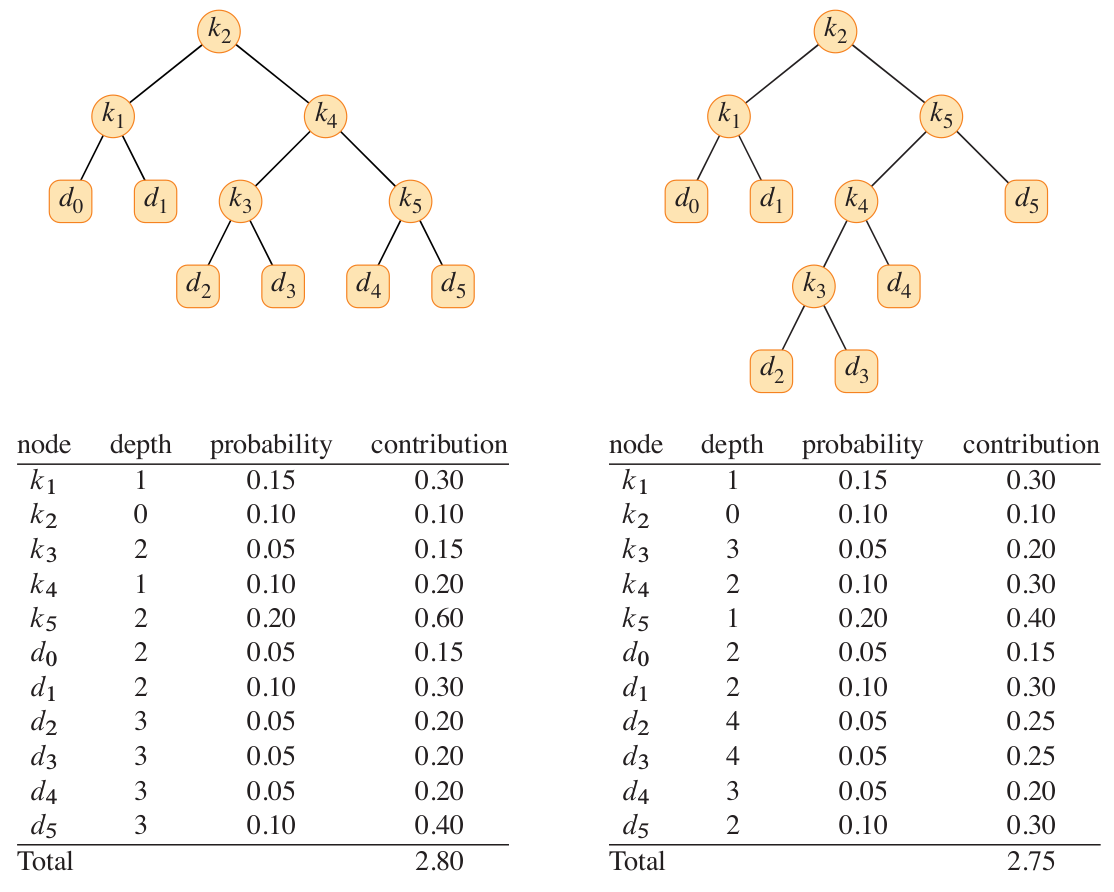
\includegraphics[width=0.6\textwidth]{figs/chap04/tree-cost}
\end{figure}
\end{itemize}
\end{frame}


\begin{frame}{‌درخت جستجوی دودویی بهینه}
\begin{itemize}\itemr
\item[-]
حال به ازای تعدادی کلید به همراه احتمال وقوع آنها، می‌خواهیم یک درخت جستجوی دودویی بیابیم که هزینهٔ جستجو در آن حداقل است.
\item[-]
به این درخت، درخت جستجوی دودویی بهینه
\fn{1}{optimal binary search tree}
گفته می‌شود.
\end{itemize}
\end{frame}


\begin{frame}{‌درخت جستجوی دودویی بهینه}
\begin{itemize}\itemr
\item[-]
در شکل زیر دو درخت جستجوی دودویی نشان داده شده‌اند. هزینهٔ جستجو در درخت سمت چپ
\m{2.80}
و در درخت سمت راست برابر با
\m{2.75}
است. درخت سمت راست یک درخت جستجوی بهینه است. در اینجا می‌توانیم ببینیم درخت جستجوی دودویی بهینه، الزاماً درختی نیست که عمق آن کمتر باشد.
\begin{figure}
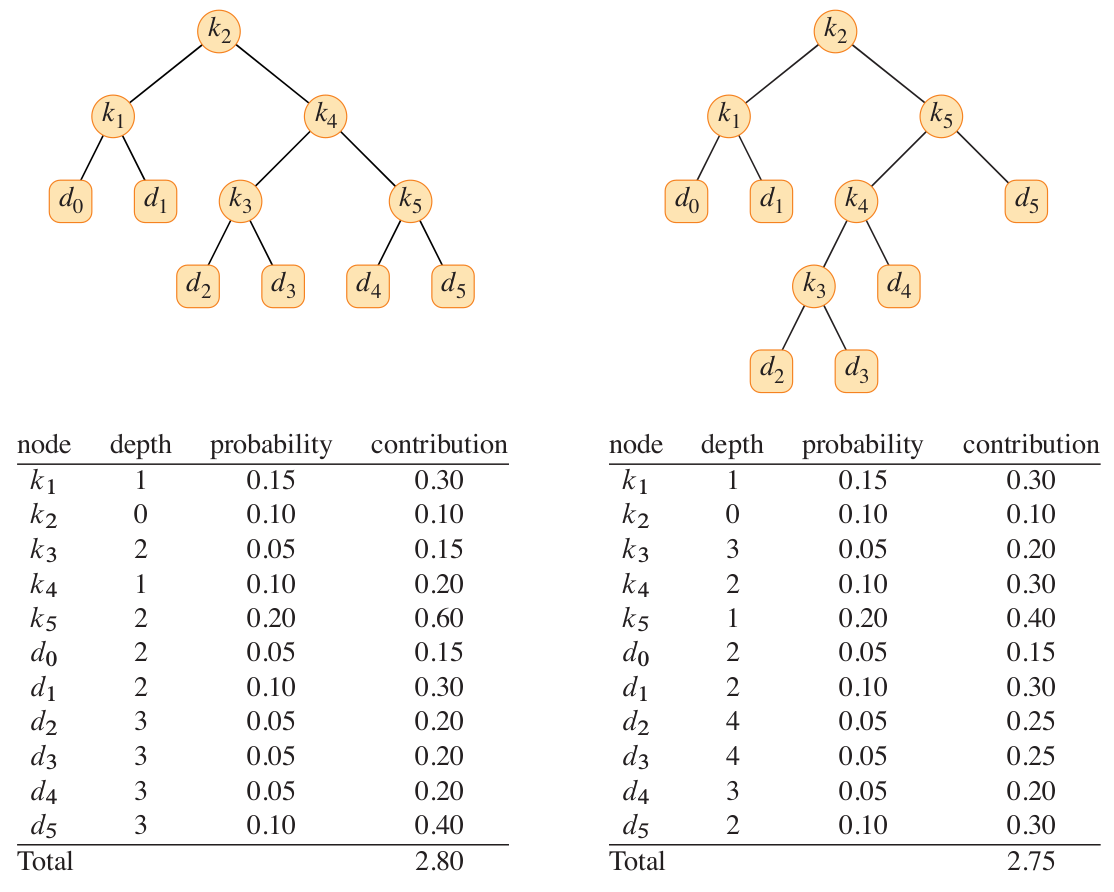
\includegraphics[width=0.5\textwidth]{figs/chap04/tree-cost}
\end{figure}
\end{itemize}
\end{frame}


\begin{frame}{‌درخت جستجوی دودویی بهینه}
\begin{itemize}\itemr
\item[-]
همچنین درخت جستجوی دودویی بهینه الزاماً درختی نیست که همهٔ کلیدها با احتمال وقوع بیشتر در ریشهٔ آن باشند. برای مثال کلید
\m{k_5}
بیشترین احتمال وقوع را دارد، اما ریشهٔ درخت جستجو
\m{k_2}
است.
\end{itemize}
\end{frame}


\begin{frame}{‌درخت جستجوی دودویی بهینه}
\begin{itemize}\itemr
\item[-]
همانند مسئله ضرب زنجیره‌ای ماتریس‌ها، با استفاده از جستجوی کامل برای بررسی همهٔ درخت‌های جستجو نمی‌توانیم در زمان چندجمله‌ای درخت جستجوی دودویی بهینه را به دست آوریم. تعداد همهٔ
 درخت‌های جستجوی دودویی از مرتبهٔ نمایی است، بنابراین بررسی همهٔ درخت‌های جستجو ممکن نیست.
\item[-]
می‌خواهیم این مسئله را با استفاده از برنامه‌ریزی پویا حل کنیم.
\end{itemize}
\end{frame}


\begin{frame}{‌درخت جستجوی دودویی بهینه}
\begin{itemize}\itemr
\item[-]
گام اول : ساختار یک درخت جستجوی دودویی بهینه
\item[-]
برای بررسی ساختار و مشخص کردن ویژگی‌های یک درخت بهینه، ابتدا ساختار درخت و زیردرخت‌های آن را بررسی می‌کنیم.
در واقع باید اثبات کنیم این مسئله دارای زیرساختار بهینه است، بدین معنی که جواب زیرمسئله‌ها را می‌توان از جواب مسئله استخراج کرد.
\item[-]
اگر یک درخت جستجوی دودویی بهینه
\m{T}
داشته باشیم، زیر درخت
\m{T'}
%شامل کلیدهای
%\m{k_i, \cdots, k_j}
%و کلیدهای
%\m{d_{i-1}, \cdots, d_j}
نیز باید بهینه باشد. اگر یک زیر درخت
\m{T''}
وجود داشت که هزینهٔ آن کمتر از
\m{T'}
بود، می‌توانستیم
\m{T'}
را با
\m{T''}
جایگزین کنیم و یک درخت با هزینه کمتر به جای
\m{T}
بیابیم که با فرض بهینه بودن
\m{T}
در تناقض است.
\item[-]
حال می‌خواهیم مسئله را با استفاده از جواب زیر مسئله‌های بهینهٔ آن حل کنیم.
\end{itemize}
\end{frame}


\begin{frame}{‌درخت جستجوی دودویی بهینه}
\begin{itemize}\itemr
\item[-]
یک زیردرخت دلخواه را در نظر بگیرید. این زیردرخت شامل کلیدهای
\m{k_i, \cdots, k_j}
است
که برگ‌های آن را کلیدهای
\m{d_{i-1}, \cdots, d_j}
تشکیل می‌دهند، به طوری‌که
\m{1 \leqslant i \leqslant j \leqslant n} .
\item[-]
به ازای کلیدهای
\m{k_i, \cdots, k_j}
، یکی از این کلیدها، برای مثال کلید
\m{k_r}
به طوری‌که
\m{i \leqslant r \leqslant j}
، ریشهٔ زیردرخت بهینه برای این کلیدهاست.
\item[-]
زیردرخت سمت چپ ریشهٔ
\m{k_r}
شامل کلیدهای
\m{k_i, \cdots, k_{r-1}}
و کلیدهای برگ
\m{d_{i-1}, \cdots, d_{r-1}}
است و زیردرخت سمت راست شامل کلیدهای
\m{k_{r+1}, \cdots, k_j}
و کلیدهای برگ
\m{d_r, \cdots, d_j}
است.
\item[-]
فرض کنید در یک زیردرخت با کلیدهای
\m{k_i, \cdots, k_j}
، کلید
\m{k_i}
را به عنوان ریشه انتخاب کنیم. 
%بنابراین زیردرخت سمت چپ این زیردرخت هیچ رأسی را شامل نمی‌شود. اگر برگ‌ها را نیز در نظر بگیریم، 
زیردرخت سمت چپ این زیردرخت یک برگ با کلید
\m{d_{i-1}}
است.
\item[-]
به طور مشابه، اگر
\m{k_j}
را به عنوان ریشه در نظر بگیریم زیر درخت سمت راست این زیر درخت شامل یک برگ با کلید
\m{d_j}
است.
\end{itemize}
\end{frame}


\begin{frame}{‌درخت جستجوی دودویی بهینه}
\begin{itemize}\itemr
\item[-]
گام دوم : راه حل بازگشتی
\item[-]
حال برای تعریف راه ‌حل بهینه به صورت بازگشتی، زیر درختی شامل کلیدهای
\m{k_i, \cdots, k_j}
را در نظر بگیرید به طوری‌که
\m{i \geqslant 1}
،
\m{j \leqslant n}
و
\m{j \geqslant i-1}
. وقتی
\m{j = i - 1}
باشد، تنها کلید برگ
\m{d_{i-1}}
را خواهیم داشت.
\item[-]
فرض کنید
\m{e[i,j]}
هزینهٔ جستجوی یک درخت جستجوی بهینه با کلیدهای
\m{k_i, \cdots, k_j}
باشد. هدف محاسبهٔ هزینه جستجو برای همهٔ کلیدهاست که برابر با مقدار
\m{e[1,n]}
می‌باشد.
\item[-]
اگر
\m{j = i - 1}
باشد، آنگاه مسئله تنها شامل یک کلید
\m{d_{i-1}}
می‌شود. در اینصورت هزینهٔ جستجو برابراست با
\m{e[i,i-1] = q_{i-1}}.
\item[-]
وقتی
\m{j \geqslant i}
باشد، باید ریشهٔ
\m{k_r}
را از بین کلیدهای
\m{k_i, \cdots, k_j}
انتخاب کنیم و یک درخت جستجوی بهینه با کلیدهای
\m{k_i, \cdots, k_{r-1}}
به عنوان زیردرخت سمت چپ ریشهٔ
\m{k_r}
و یک درخت جستجوی بهینه با کلیدهای
\m{k_{r+1}, \cdots, k_j}
به عنوان زیردرخت سمت راست ریشهٔ
\m{k_r}
بسازیم.
\end{itemize}
\end{frame}


\begin{frame}{‌درخت جستجوی دودویی بهینه}
\begin{itemize}\itemr
\item[-]
وقتی یک زیردرخت بهینه 
\m{T'}
 به عنوان زیردرخت یک رأس قرار می‌گیرد و درخت
\m{T}
را تشکیل می‌دهد،
 درواقع عمق هر یک از رأس‌های 
\m{T'}
در درخت
\m{T}
  یک واحد افزوده می‌شود. در اینصورت هزینهٔ جستجو برای رئوس زیردرخت
\m{T'}
در درخت
\m{T}
   به میزان مجموع احتمال رئوس 
\m{T'}
    افزایش می‌یابد.
\end{itemize}
\end{frame}

\begin{frame}{‌درخت جستجوی دودویی بهینه}
\begin{itemize}\itemr
\item[-]
برای مثال فرض کنید درخت
\m{T'}
 با کلید‌های
\m{k_1,k_2,k_3}
را تشکیل داده باشیم. هزینه جستجوی این درخت (بدون در نظر گرفتن کلیدهای بی‌استفاده) برابر است با
\m{E[T'] = \sum_{i=1}^3 (\depth_{T'}(k_i)+1) \cdot p_{i}  } .
\item[-]
اگر زیردرخت 
\m{T'}
در درخت 
\m{T}
قرار بگیرد به طوری که ریشه درخت 
\m{T}
کلید
\m{k_4}
و
\m{T'}
زیردرخت سمت چپ در درخت 
\m{T}
باشد، آنگاه خواهیم داشت:
\begin{align*}
\m{E[T]} =& \m{~p_4 + \Big(\sum_{i=1}^3 (\depth_{T}(k_i)+1 ) \cdot p_{i} \Big)} \\
=& \m{~p_4 + \Big( \sum_{i=1}^3 (\depth_{T'}(k_i)+2) \cdot p_{i} \Big) } \\
=& \m{~p_4 + E[T'] + \Big( \sum_{i=1}^3 p_{i} \Big) }
\end{align*}
\end{itemize}
\end{frame}

\begin{frame}{‌درخت جستجوی دودویی بهینه}
\begin{itemize}\itemr
\item[-]
برای یک زیردرخت با کلیدهای
\m{k_i, \cdots, k_j}
مجموع  احتمال‌ها برابر است با :
\begin{align*}
\m{w(i,j) = \sum_{l=i}^j p_l + \sum_{l=i-1}^j q_l}
\end{align*}
\item[-]
بنابراین اگر
\m{k_r}
ریشهٔ یک زیردرخت بهینه با کلیدهای
\m{k_i, \cdots, k_j}
باشد، خواهیم داشت :
\begin{align*}
\m{e[i,j] = p_r + (e[i,r-1] + w(i,r-1)) + (e[r+1,j] + w(r+1,j))}
\end{align*}
\end{itemize}
\end{frame}

\begin{frame}{‌درخت جستجوی دودویی بهینه}
\begin{itemize}\itemr
\item[-]
 از آنجایی که مجموع احتمال وقوع همهٔ رئوس در یک درخت برابر است با مجموع احتمال‌های وقوع رئوس زیردرخت چپ به علاوهٔ احتمال وقوع ریشه به علاوهٔ احتمال‌های وقوع رئوس زیردرخت راست، بنابراین رابطه زیر برقرار است :
\begin{align*}
\m{w(i,j) = w(i,r-1) + p_r + w(r+1,j)}
\end{align*}
\item[-]
بنابراین می‌توانیم رابطه بازگشتی برای محاسبه هزینهٔ جستجو در درخت بهینه را به صورت زیر بازنویسی کنیم :
\begin{align*}
\m{e[i,j] = e[i,r-1] + e[r+1,j] + w(i,j)}
\end{align*}
\end{itemize}
\end{frame}


\begin{frame}{‌درخت جستجوی دودویی بهینه}
\begin{itemize}\itemr
\item[-]
در اینجا فرض کردیم که می‌دانیم کدام رأس به عنوان رأس ریشهٔ
\m{k_r}
انتخاب می‌شود.
\item[-]
از آنجایی که هدف این است که ریشه‌ای را انتخاب کنیم که مقدار هزینه جستجو را کاهش دهد، بنابراین رابطهٔ بازگشتی برای محاسبهٔ هزینه جستجو در درخت بهینه را به صورت زیر می‌نویسیم.
\begin{align*}
\m{e[i,j]} = \left\{ \begin{array}{lr}
					\m{q_{i-1}} & \m{j=i-1}~~\text{اگر}\\
					\m{\min\{e[i,r-1] + e[r+1,j] + w(i,j) : i \leqslant r \leqslant j \}} & \m{i \leqslant j}~~ \text{اگر}
					\end{array}\right.
\end{align*}
\item[-]
بنابراین رابطه‌ای برای جدول
\m{e[i,j]}
جهت استفاده در یک الگوریتم برنامه‌ریزی پویا به صورت بازگشتی محاسبه کردیم.
\end{itemize}
\end{frame}


\begin{frame}{‌درخت جستجوی دودویی بهینه}
\begin{itemize}\itemr
\item[-]
جدول
\m{e[i,j]}
 تنها میزان هزینه جستجوی بهینه را نگهداری می‌کند.
\item[-]
 به یک جدول دیگر نیاز داریم برای اینکه بتوانیم ساختار درخت را نیز نگهداری کنیم تا در نهایت بتوانیم درخت جستجو بهینه را بازسازی کنیم.
\item[-]
این اطلاعات را در جدول
\m{root[i,j]}
نگهداری می‌کنیم. درواقع مقدار
\m{root[i,j]}
به ازای
\m{1 \leqslant i \leqslant j \leqslant n}
برابراست با اندیس r برای کلید
\m{k_r}
که ریشهٔ درخت جستجوی بهینه‌ای است که برای کلیدهای
\m{k_i, \cdots, k_j}
یافته می‌شود.
\end{itemize}
\end{frame}


\begin{frame}{‌درخت جستجوی دودویی بهینه}
\begin{itemize}\itemr
\item[-]
گام سوم : محاسبهٔ هزینهٔ جستجو در یک درخت جستجوی دودویی بهینه
\item[-]
حال با استفاده از روش برنامه‌ریزی پویا می‌توانیم مقادیر
\m{e[i,j]}
را به ترتیب از پایین به بالا محاسبه می‌کنیم. بنابراین کل جدول را به ازای
\m{e[1:n+1,0:n]}
مقداردهی می‌کنیم.
\item[-]
اندیس اول از 
\m{1}
 شروع شده و با
\m{n+1}
خاتمه می‌یابد، زیرا برای داشتن یک زیردرخت شامل تنها کلید
\m{d_n}
نیاز داریم
\m{e[n+1,n]}
را محاسبه کنیم. اندیس دوم باید از صفر شروع شود، زیرا برای داشتن یک زیردرخت تنها با کلید
\m{d_0}
، باید مقدار
\m{e[1,0]}
را محاسبه کنیم.
\item[-]
همهٔ مقادیر
\m{e[i,j]}
به ازای
\m{j \geqslant i-1}
باید محاسبه شوند. جدول
\m{root[i,j]}
ریشهٔ زیردرخت‌ها را با کلیدهای
\m{k_i, \cdots, k_j}
ذخیره می‌کند، به طوری‌که
\m{1 \leqslant i \leqslant j \leqslant n}.
\end{itemize}
\end{frame}


\begin{frame}{‌درخت جستجوی دودویی بهینه}
\begin{itemize}\itemr
\item[-]
همچنین می‌توانیم از یک جدول دیگر بهره بگیریم تا محاسبات را سریع‌تر انجام دهیم.
\item[-]
به جای محاسبه
\m{w(i,j)}
برای هر یک از درایه‌های
\m{e[i,j]}
%که به زمان
%\ath{j-i}
%نیاز دارد، 
جدول
\m{w[1:n+1,0:n]}
را محاسبه می‌کنیم. در حالت پایه، مقدار
\m{w[i,i-1] = q_{i-1}}
به ازای
\m{1 \leqslant i \leqslant n+1}
\item[-]
به ازای
\m{j \geqslant i}
درایه‌های جدول w را به صورت زیر محاسبه می‌کنیم.
\begin{align*}
\m{w[i,j] = w[i,j-1] + p_j + q_j}
\end{align*}
\item[-]
بنابراین می‌توانیم
\ath{n^2}
مقدار
\m{w[i,j]}
را هرکدام در زمان
\ath{1}
محاسبه کنیم.
% و مقادیر ذخیره شده در جدول را در زمان اجرا بازیابی کنیم.
\end{itemize}
\end{frame}


\begin{frame}{‌درخت جستجوی دودویی بهینه}
\begin{itemize}\itemr
\item[-]
الگوریتم زیر مسئلهٔ درخت جستجوی دودویی بهینه را به روش برنامه‌ریزی پویا حل می‌کند.
\begin{algorithm}[H]\alglr
  \caption{Optimal-BST} 
  \begin{algorithmic}[1]
   \Func{Optimal-BST}{p, q, n}
    \State let e[1:n+1 , 0:n], w[1:n+1 , 0:n], and root[1:n , 1:n] be new tables
    \For{i = 1 \To n + 1} \LeftComment{base cases} 
      \State e[i,i-1] = q[i-1]
      \State w[i,i-1] = q[i-1]
    \EndFor                        
  \end{algorithmic}
  \label{alg:merge}
\end{algorithm}
\end{itemize}
\end{frame}


\begin{frame}{‌درخت جستجوی دودویی بهینه}
\begin{itemize}\itemr
\item[-]
\begin{algorithm}[H]\alglr
  \caption{Optimal-BST} 
  \begin{algorithmic}[1]
  \setcounter{ALG@line}{4}
   \Func{Optimal-BST}{p, q, n}
    \For{t = 1 \To n}
    	\For{i = 1 \To n - t + 1}
    		\State j = i + t - 1
    		\State e[i,j] = $\infty$
    		\State w[i,j] = w[i,j-1] + p[j] + q[j]
    		 \For{r = i \To j} \LeftComment{try all possible roots r}
    		 		\State t = e[i,r-1] + e[r+1,j] + w[i,j] 
    		 		\If{t < e[i,j]} \LeftComment{new minimum?}
    		 				\State e[i,j] = t
    		 				\State root[i,j] = r
    		 		\EndIf
    		 \EndFor
    	\EndFor
    \EndFor
   \State \Return e and root                         
  \end{algorithmic}
  \label{alg:merge}
\end{algorithm}
\end{itemize}
\end{frame}


\begin{frame}{‌درخت جستجوی دودویی بهینه}
\begin{itemize}\itemr
\item[-]
الگوریتم درخت جستجوی دودویی بهینه محاسبات را در زمان
\ath{n^3}
انجام می‌دهد و به یک جدول با اندازهٔ
\ath{n^2}
نیاز دارد.
\end{itemize}
\end{frame}


\begin{frame}{‌درخت جستجوی دودویی بهینه}
\begin{itemize}\itemr
\item[-]
در شکل زیر، جدول‌های
\m{e[i,j]}
،
\m{w[i,j]}
و
\m{root[i,j]}
با استفاده از الگوریتم برنامه‌ریزی پویا برای جستجوی دودویی بهینه برای کلید‌های تعیین شده زیر، محاسبه شده‌اند.
\begin{figure}
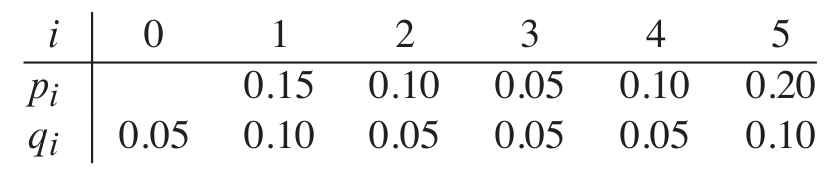
\includegraphics[width=0.5\textwidth]{figs/chap04/key-prob-example}
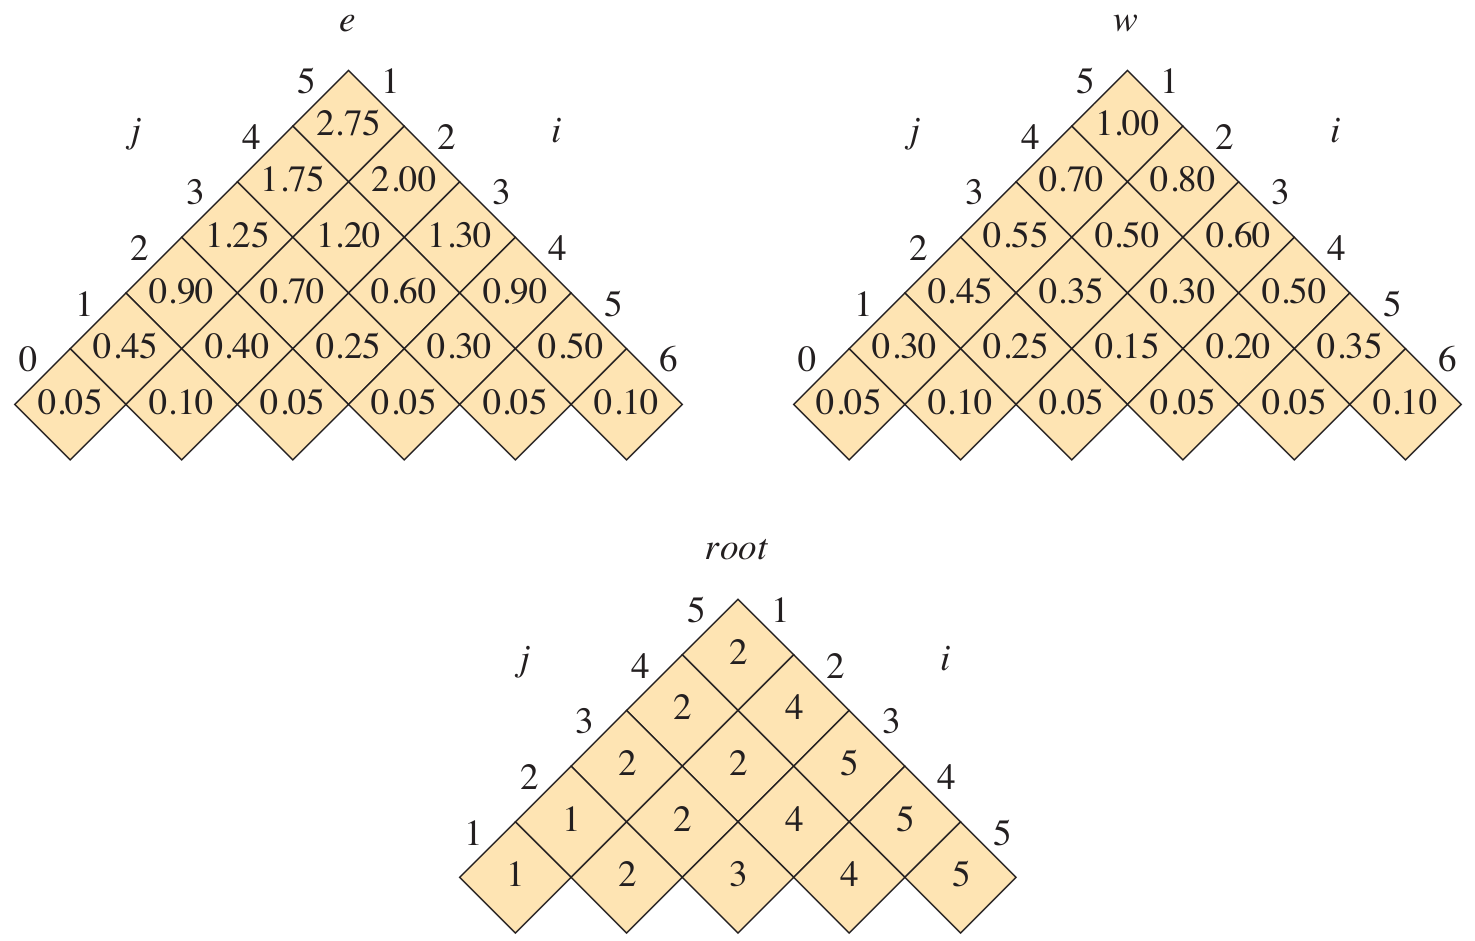
\includegraphics[width=0.5\textwidth]{figs/chap04/bst-example}
\end{figure}
\end{itemize}
\end{frame}
\newcommand{\itm}{\text{item}}
\begin{frame}{‌کوله‌پشتی ۱-۰}
\begin{itemize}\itemr
\item[-]
یک دزد با یک کوله‌پشتی به یک فروشگاه دستبرد می‌زند. وزنی که کوله‌پشتی او می‌تواند تحمل کند
\m{W}
است. در این فروشگاه تعداد
\m{n}
کالا وجود دارد. هر کالای
\m{\itm_i}
دارای وزن
\m{w_i}
و ارزش
\m{v_i}
است. دزد می‌خواهد از میان این کالاها تعدادی را انتخاب کرده در کوله‌پشتی خود قرار دهد به طوری‌که مجموع وزن کالاهای انتخاب شده از ظرفیت کوله‌پشتی یعنی
\m{W}
بیشتر نباشد و مجموع ارزش کالاهای دزدیده شده حداکثر باشد.
\item[-]
بنابراین دزد می‌خواهد از مجموعهٔ
\m{S = \{\itm_1 ,\itm_2 , \cdots ,\itm_n \} }
یک زیر مجموعه
\m{A}
را انتخاب کند به طور
\m{\sum_{\itm_i \in A} v_i}
بیشترین مقدار ممکن باشد و
\m{(\sum_{\itm_i \in A} w_i) \leqslant W}
باشد.
\item[-]
تعداد همهٔ حالت‌های ممکن تعداد همهٔ زیر مجموعه‌های
\m{S}
است که برابر است با
\m{2^n}
جایی که
\m{n}
تعداد کالاهاست.
\item[-]
در این مسئله دزد یا می‌تواند یک کالا را بردارد یا بگذارد و امکان شکستن کالاها به دو قسمت وجود ندارد. به همین دلیل به آن مسئله کوله پشتی ۱-۰
\fn{1}{\m{0}-\m{1} knapsack}
گفته می‌شود. در مسئلهٔ کوله‌پشتی کسری
\fn{2}{fractional knapsack}
دزد می‌تواند یک کالا را به دو قسمت تقسیم کرده، یک قسمت را در کوله‌پشتی قرار دهد و قسمت دیگر را در فروشگاه بگذارد.
\end{itemize}
\end{frame}


\begin{frame}{‌کوله‌پشتی ۱-۰}
\begin{itemize}\itemr
\item[-]
در گام اول باید اثبات کنیم این مسئله دارای زیر ساختار بهینه است یا به عبارت دیگر قانون بهینگی
\fn{1}{principle of optimality}
برای آن صادق است.
\item[-]
فرض کنید
\m{A}
زیر مجموعه بهینه از
\m{n}
کالا باشد. دو حالت وجود دارد : یا
\m{A}
شامل
\m{\itm_n}
می‌شود یا خیر.
\item[-]
اگر
\m{A}
کالای
\m{\itm_n}
را شامل نشود،
\m{A}
یک زیر مجموعه بهینه برای
\m{n-1}
کالا نیز هست.
\item[-]
اگر
\m{A}
کالای
\m{\itm_n}
را شامل شود، آنگاه مجموع ارزش‌های کالاهای
\m{A}
برابر است با
\m{v_n}
به علاوه بیشترین ارزش ممکن که از
\m{n-1}
کالا برای یک کوله‌پشتی با ظرفیت
\m{W-w_n}
به دست آمده است. این گزاره‌ها را می‌توانیم با برهان خلف اثبات کنیم.
\end{itemize}
\end{frame}


\begin{frame}{‌کوله‌پشتی ۱-۰}
\begin{itemize}\itemr
\item[-]
در گام دوم باید یک رابطه بازگشتی برای محاسبه جواب مسئله براساس جواب زیر مسئله‌ها بنویسیم.
\item[-]
%اگر
%\m{i > 0}
%و
%\m{w > 0}
%باشد آنگاه
فرض کنید
\m{P[i][w]}
بیشترین ارزش به دست آمده از
\m{i}
کالای اول است وقتی که ظرفیت کوله‌پشتی
\m{w}
باشد.
\item[-]
می‌توانیم یک رابطه بازگشتی به صورت زیر برای محاسبه
\m{P[i][w]}
بنویسیم.
\begin{align*}
\m{P[i][w]} = \left\{\begin{array}{lr}
          \m{\max (P[i-1][w] , v_i + P[i-1][w-w_i])}&\m{w_i \leqslant w}~\text{اگر}\\
          \m{P[i-1][w]}&\m{w_i > w}~\text{اگر}
\end{array}\right.
\end{align*}
\item[-]
در این مسئله به دنبال
\m{P[n][W]}
می‌گردیم.
\end{itemize}
\end{frame}


\begin{frame}{‌کوله‌پشتی ۱-۰}
\begin{itemize}\itemr
\item[-]
می‌توانیم جدولی تشکیل دهیم که هر سطر
\m{i}
در آن نشان دهنده این باشد که فقط از
\m{i}
کالای اول استفاده کرده‌ایم و ستون‌های آن همهٔ وزن‌های ممکن از
\m{0}
تا
\m{W}
باشد.
\item[-]
مقادیر
\m{P[0][w]}
و
\m{P[i][0]}
برابر با صفر هستند.
\item[-]
این جدول دارای
\m{nW}
خانه است پس محاسبه این جدول در زمان
\ath{nW}
امکان‌پذیر است.
\end{itemize}
\end{frame}


\begin{frame}{‌کوله‌پشتی ۱-۰}
\begin{itemize}\itemr
\item[-]
توجه کنید که هیچ رابطه‌ای بین
\m{n}
و
\m{W}
وجود ندارد و این الگوریتم می‌تواند از الگوریتمی که همه حالات را بررسی می‌کند بدتر باشد. برای مثال اگر
\m{W = n!}
باشد الگوریتم برنامه‌ریزی پویا از مرتبه
\m{n!}
است درحالی که بررسی همه حالات در زمان
\ath{2^n}
امکان‌پذیر است.
\item[-]
بنابراین تنها در صورتی از برنامه‌ریزی پویا استفاده می‌کنیم که
\m{nW < 2^n}
باشد.
\item[-]
پیچیدگی زمانی
\ath{nW}
گرچه شبیه به پیچیدگی زمانی چندجمله‌ای است، اما در واقع چندجمله‌ای نیست و مقدار 
\m{W}
می‌تواند یک تابع غیرچندجمله‌ای از ورودی مسئله باشد. این پیچیدگی زمانی را پیچیدگی زمانی شبه‌چندجمله‌ای
\fn{1}{pseudo-polynomial time complexity}
می‌نامیم.
\end{itemize}
\end{frame}

\begin{frame}{‌سریع‌ترین مسیر در جدول}
\begin{itemize}\itemr
\item[-]
جدول
\m{A}
با
\m{m}
سطر و
\m{n}
ستون را در نظر بگیرید به طوری‌که مقدار هرکدام از درایه‌های جدول یک عدد صحیح است.
\item[-]
می‌خواهیم مهره‌ای را با شروع از درایه
\m{(1,1)}
حرکت داده، به درایهٔ
\m{(m,n)}
منتقل کنیم. فرض کنید درایهٔ
\m{(1,1)}
در شمال غرب و درایهٔ
\m{(m,n)}
در جنوب شرق جدول قرار دارد.
\item[-]
وقتی مهره وارد درایهٔ
\m{(i,j)}
می‌شود، باید
\m{A[i,j]}
ثانیه در آن درایه صبر کند و پس از آن به حرکت ادامه دهد.
\item[-]
با فرض اینکه مهره تنها می‌تواند به سمت جنوب یا شرق یا مورب به جنوب شرق حرکت کند، می‌خواهیم کمترین زمان ممکن برای انتقال مهره از درایهٔ
\m{(1,1)}
به
\m{(m,n)}
را محاسبه کنیم.
\end{itemize}
\end{frame}


\begin{frame}{‌سریع‌ترین مسیر در جدول}
\begin{itemize}\itemr
\item[-]
در گام اول بررسی می‌کنیم مسئله دارای زیر ساختار بهینه است یا اصل بهینگی در آن برقرار است.
\item[-]
اگر از درایهٔ
\m{(1,1)}
مهره را حرکت داده در کمترین زمان ممکن به درایهٔ
\m{(i,j)}
برسیم حتما از یکی از سه درایهٔ
\m{(i-1,j)}
یا
\m{(i,j-1)}
یا
\m{(i-1,j-1)}
عبور کرده‌ایم.
\item[-]
در صورتی که از
\m{(i-1,j)}
عبور کرده باشیم الزاما برای حرکت از درایه
\m{(1,1)}
به
\m{(i-1,j)}
کمترین زمان ممکن را صرف کرده‌ایم. این گزاره را می‌توانیم با برهان خلف اثبات کنیم.
\item[-]
به همین ترتیب ممکن است از درایه‌های
\m{(i,j-1)}
یا
\m{(i-1,j-1)}
عبور کرده باشیم که به طور مشابه می‌توانیم اثبات کنیم الزاما در کمترین زمان ممکن به این درایه‌ها رسیده‌ایم.
\end{itemize}
\end{frame}


\begin{frame}{‌سریع‌ترین مسیر در جدول}
\begin{itemize}\itemr
\item[-]
در گام دوم رابطه‌ای برای توصیف جواب مسئله براساس جواب زیر مسئله‌ها به صورت زیر می‌نویسیم.
\begin{align*}
\m{T[i,j]} = \left\{\begin{array}{lr}
          \m{\min(T[i-1,j],T[i,j-1],T[i-1,j-1]) + A[i,j]}&\m{j > 1 , i > 1}~\text{اگر}\\
          \m{T[i-1,1] + A[i,1]}&\m{j = 1 , i > 1}~\text{اگر}\\
          \m{T[1,j-1] + A[1,j]}&\m{i = 1 , j > 1}~\text{اگر}\\
          \m{A[1,1]}&\m{j = 1 , i = 1}~\text{اگر}
\end{array}\right.
\end{align*}
\end{itemize}
\end{frame}


\begin{frame}{‌سریع‌ترین مسیر در جدول}
\begin{itemize}\itemr
\item[-]
سپس جدول
\m{T}
را در زمان
\ath{mn}
تکمیل می‌کنیم و
\m{T[m,n]}
جواب مسئله است.
\end{itemize}
\end{frame}
%%%%%%%%%%%%%%%%%%%%%%%%%
\section{الگوریتم‌های حریصانه}
%%%%%%%%%%%%%%%%%%%%%%%%%

\begin{frame}{‌الگوریتم‌های حریصانه}
\begin{itemize}\itemr
\item[-]
مسئله‌های بهینه‌سازی به دنبال جواب بهینه در مجموعه‌ای از جواب‌ها برای یک مسئله می‌گردند. یک جواب بهینه جوابی است که در یک معیار اندازه‌گیری بهترین باشد. برای مثال یک جواب بهینه می‌تواند کوچک‌ترین، بزرگ‌ترین، کوتاهترین، بلندترین و غیره باشد.
\item[-]
برنامه‌ریزی پویا یکی از روش‌ها برای حل مسئله‌های بهینه‌سازی است.
\item[-]
الگوریتم‌های حریصانه
\fn{1}{greedy algorithms}
دسته‌ای دیگر از الگوریتم‌ها برای حل مسئله‌های بهینه‌سازی هستند.
\end{itemize}
\end{frame}


\begin{frame}{‌الگوریتم‌های حریصانه}
\begin{itemize}\itemr
\item[-]
فرض کنید می‌خواهیم در مدت
\m{n}
روز به بیشترین دارایی ممکن دست پیدا کنیم.
برای این کار کافی است که در هر روز بیشترین دارایی ممکن را کسب کنیم.
بنابراین برای به دست آوردن بیشترین دارایی در مدت
\m{n}
روز باید در روز اول بیشترین دارایی را کسب کنیم و زیر مسئله‌ای که باید در گام بعد حل شود این است که چگونه در مدت
\m{n-1}
روز بیشترین دارایی را کسب کنیم.
پس در هر روز یک انتخاب حریصانه انجام می‌دهیم و آن انتخاب، کسب بیشترین دارایی در همان روز است. می‌دانیم که با این انتخاب حریصانه در مدت
\m{n}
روز بیشترین دارایی را کسب خواهیم کرد.
\item[-]
یک الگوریتم حریصانه مسئله را از بالا به پایین حل می‌کند. برای حل یک مسئله به روش حریصانه در هر گام یک انتخاب بهینه انجام می‌شود و از یک مسئله یک زیرمسئله به دست می‌آید.
این فرایند ادامه پیدا می‌کند تا زیرمسئله‌ای باقی نماند. در پایان جواب مسئله مجموعهٔ همهٔ انتخاب‌های بهینه است.
به عبارت دیگر در هر گام یک انتخاب حریصانه برای به دست آوردن جواب بهینه صورت می‌گیرد و در پایان مجموعهٔ همهٔ انتخاب‌های حریصانه جواب مسئله است.
% و در هر گام الگوریتم انتخاب‌هایی می‌کند تا به پاسخ بهینه برسد. در الگوریتم‌های حریصانه 
% در هر گام، الگوریتم بهینه‌ترین انتخاب را انجام می‌دهد به این امید که در پایان جواب بهینه به دست آید.
%\item[-]
%الگوریتم‌های حریصانه تنها در برخی از مسائل با ویژگی‌های خاص به پاسخ بهینه دست می‌یابند.
\end{itemize}
\end{frame}


\begin{frame}{‌الگوریتم‌های حریصانه}
\begin{itemize}\itemr
\item[-]
تنها برخی از مسئله‌های بهینه‌سازی را می‌توان به روش حریصانه حل کرد.
\item[-]
برای مثال مسئله درخت جستجوی دودویی بهینه را در نظر بگیرید. اگر در هر گام برای ساختن درخت جستجوی دودویی بهینه از بین همهٔ کلیدها، کلیدی را به عنوان ریشه در نظر بگیریم که بیشترین احتمال وقوع را داشته باشد، درخت به دست آمده الزاما بهینه نیست.
\item[-]
همانطور که مشاهده کردیم ریشهٔ یک درخت جستجوی دودویی بهینه ممکن است کلیدی باشد که بیشترین احتمال وقوع را نداشته باشد.
%\item[-]
%در صورتی یک مسئله را می‌توان به روش حریصانه حل کرد که پس از نوشتن رابطه بازگشتی، تنها یک زیرمسئله جواب مسئله باشد.
\end{itemize}
\end{frame}

\begin{frame}{‌مسئله انتخاب فعالیت‌ها}
\begin{itemize}\itemr
\item[-]
در مسئله انتخاب فعالیت‌ها
\fn{1}{activity selection problem}
، تعدادی فعالیت به طور همزمان می‌خواهند انجام شوند به طوری‌که این فعالیت‌ها از یک منبع مشترک استفاده می‌کنند و این منبع مشترک نمی‌تواند به طور همزمان توسط فعالیت‌ها استفاده شود. می‌خواهیم مجموعه‌ای از فعالیت‌ها را انتخاب کنیم، به طوری که بیشترین تعداد فعالیت‌ها بتوانند اجرا شوند.
\item[-]
فرض کنید شما مسئول زمانبندی یک اتاق کنفرانس هستید. به شما مجموعهٔ
\m{S = \{a_1,a_2, \cdots, a_n \}}
شامل n فعالیت داده شده است که می‌خواهند اتاق کنفرانس را رزرو کنند. در این اتاق در یک زمان تنها یک فعالیت می‌تواند صورت بگیرد.
\end{itemize}
\end{frame}


\begin{frame}{‌مسئله انتخاب فعالیت‌ها}
\begin{itemize}\itemr
\item[-]
هر فعالیت
\m{a_i}
یک زمان شروع
\fn{1}{state time}
\m{s_i}
و یک زمان پایان
\fn{2}{finish time}
\m{f_i}
دارد به طوری‌که
\m{0 \leqslant s_i < f_i < \infty}.
اگر فعالیت
\m{a_i}
انتخاب شود، آنگاه این فعالیت می‌تواند در بازهٔ زمانی
\m{[s_i,f_i)}
انجام شود. دو فعالیت
\m{a_i}
و
\m{a_j}
سازگار
\fn{3}{compatible}
گفته می‌شوند اگر بازه‌های زمانی
\m{[s_i,f_i)}
و
\m{[s_j,f_j)}
تداخل نداشته باشند. دو فعالیت تداخل ندارند اگر
\m{s_i \geqslant f_j}
یا
\m{s_j \geqslant f_i}
. در مسئلهٔ انتخاب فعالیت‌ها، هدف این است که بیشترین تعداد فعالیت‌های سازگار از یک مجموعهٔ فعالیت‌ها انتخاب شوند.
\item[-]
فرض می‌کنیم فعالیت‌ها بر اساس زمان پایان‌شان مرتب شده‌اند. به عبارت دیگر :
\begin{align*}
\m{f_1 \leqslant f_2 \leqslant f_3 \leqslant \cdots \leqslant f_{n-1} \leqslant f_n}
\end{align*}
\end{itemize}
\end{frame}


\begin{frame}{‌مسئله انتخاب فعالیت‌ها}
\begin{itemize}\itemr
\item[-]
برای مثال مجموعه‌ای از فعالیت‌ها در جدول زیر را در نظر بگیرید.
\begin{figure}
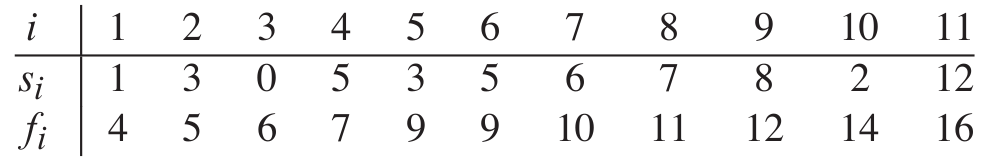
\includegraphics[width=0.7\textwidth]{figs/chap05/activity-example}
\end{figure}
\item[-]
مجموعهٔ
\m{\{a_3,a_9,a_{11}\}}
مجموعه‌ای از فعالیت‌های سازگار است ولی بزرگ‌ترین مجموعهٔ فعالیت‌های سازگار نیست چراکه
\m{\{a_1,a_4,a_8,a_{11}\}}
تعداد بیشتری فعالیت را شامل می‌شود.
همچنین مجموعهٔ
\m{\{a_2,a_4,a_9,a_{11}\}}
تعداد چهار فعالیت را شامل می‌شود.
\end{itemize}
\end{frame}



\begin{frame}{‌مسئله انتخاب فعالیت‌ها}
\begin{itemize}\itemr
\item[-]
در اینجا ابتدا سعی می‌کنیم مسئلهٔ انتخاب فعالیت‌ها را توسط برنامه‌ریزی پویا حل کنیم.
\item[-]
 فرض کنید
\m{S_{ij}}
مجموعه‌ای از فعالیت‌ها باشد که پس از اتمام فعالیت
\m{a_i}
آغاز
و قبل از شروع فعالیت
\m{a_j}
تمام می‌شوند.
فرض کنید می‌خواهیم حداکثر فعالیت‌های سازگار
\m{S_{ij}}
را پیدا کنیم و فرض کنید
\m{A_{ij}}
مجموعه‌ای است که شامل حداکثر تعداد فعالیت‌های سازگار از مجموعهٔ
\m{S_{ij}}
است.
\item[-]
حال فرض کنید
\m{a_k}
یکی از فعالیت‌ها در مجموعهٔ
\m{A_{ij}}
است. در اینجا دو زیر مسئله داریم : مسئلهٔ یافتن حداکثر فعالیت‌های سازگار در
\m{S_{ik}}
(که شامل فعالیت‌هایی می‌شود که پس از اتمام
\m{a_i}
آغاز
و قبل از شروع
\m{a_k}
پایان می‌یابند) و مسئلهٔ یافتن حداکثر فعالیت‌های سازگار در
\m{S_{kj}}
(که شامل فعالیت‌هایی می‌شود که پس از اتمام
\m{a_k}
آغاز
و قبل از شروع
\m{a_j}
پایان می‌یابند).
\end{itemize}
\end{frame}

\begin{frame}{‌مسئله انتخاب فعالیت‌ها}
\begin{itemize}\itemr
\item[-]
در گام اول باید ثابت کنیم مسئله دارای زیرساختار بهینه است.
\item[-]
 فرض کنید
\m{a_k}
در مجموعهٔ جواب
\m{A_{ij}}
است.
حال فرض کنید
\m{A_{ik} = A_{ij}\cap S_{ik}}
و
\m{A_{kj} = A_{ij}\cap S_{kj}},
بنابراین
\m{A_{ik}}
شامل فعالیت‌هایی در
\m{A_{ij}}
می‌شود که قبل از شروع
\m{a_k}
پایان می‌یابند و
\m{A_{kj}}
شامل فعالیت‌هایی در
\m{A_{ij}}
می‌شود که پس از اتمام
\m{a_k}
شروع می‌شوند.
\item[-]
اگر
\m{a_k}
در 
\m{A_{ij}}
باشد، الزاما
\m{A_{ik}}
جواب مسئله
\m{S_{ik}}
و
\m{A_{kj}}
جواب مسئله
\m{S_{kj}}
است.
\item[-]
با استفاده از برهان خلف می‌توانیم اثبات کنیم پاسخ بهینه برای
\m{S_{ij}}
شامل پاسخ بهینه برای دو زیر مسئله
\m{S_{ik}}
و
\m{S_{kj}}
می‌شود. اگر می‌توانستیم مجموعه
\m{A'_{kj}}
از حداکثر فعالیت‌های سازگار
\m{S_{kj}}
را پیدا کنیم به طوری‌که
\m{|A'_{kj}| > |A_{kj}|}
آنگاه می‌توانستیم از
\m{A'_{kj}}
به جای
\m{A_{kj}}
در زیر مسئلهٔ
\m{S_{ij}}
استفاده کنیم و بنابراین داشتیم :\\
\m{|A_{ik}| + |A'_{kj}| + 1 > |A_{ik}| + |A_{kj}| + 1 = |A_{ij}|}
که با فرض اینکه
\m{A_{ij}}
جواب بهینه است در تناقض است.
\end{itemize}
\end{frame}

\begin{frame}{‌مسئله انتخاب فعالیت‌ها}
\begin{itemize}\itemr
\item[-]
طبق تعریف می‌دانیم
حداکثر تعداد فعالیت‌ها در 
\m{S_{ik}}
برابر است با
\m{A_{ik}}
و
حداکثر تعداد فعالیت‌ها در 
\m{S_{kj}}
برابر است با
\m{A_{kj}} .
\item[-]
بنابراین داریم
\m{A_{ij} = A_{ik}\cup \{a_k \} \cup A_{kj}}
و در نتیجه
\m{|A_{ij}| = |A_{ik}| + |A_{kj}| + 1}.
\end{itemize}
\end{frame}


\begin{frame}{‌مسئله انتخاب فعالیت‌ها}
\begin{itemize}\itemr
\item[-]
فرض کنید اندازه مجموعه جواب بهینه برای
\m{S_{ij}}
را با
\m{c[i,j]}
نشان دهیم، 
بنابراین 
\m{|A_{ij}| = c[i,j]} .
\item[-]
آنگاه می توانیم بنویسیم :
\m{c[i,j] = c[i,k] + c[k,j] + 1}.
\item[-]
از آنجایی که نمی‌دانیم به ازای کدام
\m{a_k}
جواب بهینه به‌دست می‌آید، بنابراین باید همهٔ
\m{a_k}
ها را در نظر بگیریم تا جواب بهینه را به دست آوریم.
\begin{align*}
\m{c[i,j] = } \left\{ \begin{array}{lr}
					\m{0} & \m{S_{ij} = \emptyset}~~\text{اگر}\\
					\m{\max \{c[i,k] + c[k,j] + 1 : a_k \in S_{ij} \}} & \m{S_{ij} \neq \emptyset}~~\text{اگر}
					\end{array}\right.
\end{align*}
\item[-]
سپس می‌توانیم این مسئله را به روش برنامه‌ریزی پویا حل کنیم.
%\item[-]
%مشاهده خواهیم کرد که به جای چند انتخاب برای زیر مسئله‌های بهینه، در این مسئله همیشه در هنگام استفاده از برنامه‌ریزی پویا، تنها یک زیرمسئلهٔ بهینه وجود دارد. انتخاب این زیرمسئلهٔ بهینه همان انتخاب حریصانه است. درواقع با یک انتخاب حریصانه در هرگام از الگوریتم در نهایت به جواب بهینه دست پیدا می‌کنیم.
\end{itemize}
\end{frame}


\begin{frame}{‌مسئله انتخاب فعالیت‌ها}
\begin{itemize}\itemr
\item[-]
می‌توانیم رابطهٔ به دست آمده را ساده‌تر کنیم.
\item[-]
در مجموعهٔ
\m{S_{ij}}
همیشه یکی از عناصر به عنوان اولین عنصری است که در مجموعهٔ
\m{A_{ij}}
قرار می‌گیرد.
\item[-]
می‌خواهیم اولین عنصر از مجموعهٔ 
\m{S_{ij}}
که در مجموعهٔ 
\m{A_{ij}}
قرار می‌گیرد را انتخاب کنیم.
\item[-]
پس صورت مسئله را تغییر می‌دهیم.
\end{itemize}
\end{frame}


\begin{frame}{‌مسئله انتخاب فعالیت‌ها}
\begin{itemize}\itemr
\item[-]
فرض کنید
\m{S_k = \{a_i  \in S : s_i \geqslant f_k \}}
مجموعه‌ای از فعالیت‌ها باشد که پس از اتمام
\m{a_k}
آغاز می‌شوند.
\item[-]
اولین فعالیت در 
\m{S_k}
که در بزرگترین مجموعهٔ سازگار فعالیت‌ها قرار می‌گیرد کدام است؟
\end{itemize}
\end{frame}

\iffalse
\begin{frame}{‌مسئله انتخاب فعالیت‌ها}
\begin{itemize}\itemr
\item[-]
انتخاب حریصانه
\m{a_1}
اولین فعالیتی است که
انتخاب می‌شود و پس از آن
\m{S_1}
زیر مسئلهٔ بعدی است که باید حل شود.
\item[-]
بنابراین اگر
\m{a_1}
متعلق به مجموعهٔ جواب بهینه باشد، آنگاه مجموعه جواب بهینه برای کل مسئله برابر است با
\m{a_1}
 و تمام فعالیت‌هایی که به جواب زیر مسئلهٔ
\m{S_1}
تعلق دارند.
\item[-]
این راه‌حل را به طور شهودی به دست آوردیم. حال باید اثبات کنیم که این راه‌حل درست است.
\end{itemize}
\end{frame}
\fi

\begin{frame}{‌مسئله انتخاب فعالیت‌ها}
\begin{itemize}\itemr
\item[-]
قضیه : فرض کنید
\m{S_k}
مجموعه‌ای غیر تهی از فعالیت‌هاست و
\m{a_m}
فعالیتی است در
\m{S_k}
که کوچک‌ترین زمان پایان را دارد. آنگاه
\m{a_m}
در بزرگ‌ترین مجموعهٔ فعالیت‌های سازگار
\m{S_k}
قرار دارد.
\item[-]
اثبات : فرض کنید
\m{A_k}
بزرگ‌ترین مجموعهٔ فعالیت‌های سازگار
\m{S_k}
باشد و
\m{a_j}
فعالیتی در
\m{A_k}
باشد که کوچکترین زمان پایان را دارد. اگر
\m{a_j = a_m}
باشد به نتیجه مطلوب رسیده‌ایم یعنی در واقع
\m{a_m}
متعلق به بزرگ‌ترین مجموعهٔ فعالیت‌های سازگار
\m{S_k}
است.
\item[-]
حال فرض کنیم
\m{a_j \neq a_m}
باشد. مجموعهٔ
\m{A'_k = (A_k - \{a_j\}) \cup \{a_m\}}
را به عنوان مجموعه‌ای که شامل
\m{a_j}
نیست ولی
\m{a_m}
را شامل می‌شود در نظر بگیرید. فعالیت‌های
\m{A'_k}
سازگار هستند، زیرا فعالیت‌های
\m{A_k}
سازگار هستند،
و
\m{a_j}
اولین فعالیت در
\m{A_k}
است که به اتمام می‌رسد و
\m{f_m \leqslant f_j}.
از آنجایی که
\m{|A'_k| = |A_k|}
، نتیجه می‌گیریم که
\m{A'_k}
نیز بزرگ‌ترین مجموعه فعالیت‌های سازگار
\m{S_k}
است که
\m{a_m}
را نیز شامل می‌شود.
\end{itemize}
\end{frame}



\begin{frame}{‌مسئله انتخاب فعالیت‌ها}
\begin{itemize}\itemr
\item[-]
فرض کنید اندازه مجموعه جواب بهینه برای
\m{S_{k}}
را با
\m{c[k]}
نشان دهیم، 
بنابراین 
\m{|A_{k}| = c[k]} .
\item[-]
اگر اولین عضو مجموعهٔ
\m{S_k}
فعالیت
\m{a_m}
باشد، طبق قضیه قبل
\m{a_m}
در
\m{A_k}
است.
  مجموعه فعالیت‌های باقیمانده
\m{S_{m}}
است و در اینصورت
می توانیم بنویسیم :
\m{c[k] = 1 + c[m]}.
\item[-]
بنابراین می‌توانیم بنویسیم:
\begin{align*}
\m{c[k] = } \left\{ \begin{array}{lr}
					\m{0} & \m{S_{k} = \emptyset}~~\text{اگر}\\
					\m{1 + c[m]} & \text{باشد.}~\m{S_k}~\text{اولین عضو}~\m{a_m}~\text{و}~\m{S_{k} \neq \emptyset}~~\text{اگر}
					\end{array}\right.
\end{align*}
\item[-]
در اینجا یک رابطهٔ بازگشتی به دست آوردیم که همیشه تنها یک انتخاب بهینه در آن وجود دارد.
در صورتی که بتوانیم چنین رابطهٔ بازگشتی برای یک مسئله پیدا کنیم، که در آن همیشه یک انتخاب بهینه وجود داشته باشد، می‌توانیم مسئله را با استفاده از روش حریصانه حل کنیم.
%\item[-]
%مشاهده خواهیم کرد که به جای چند انتخاب برای زیر مسئله‌های بهینه، در این مسئله همیشه در هنگام استفاده از برنامه‌ریزی پویا، تنها یک زیرمسئلهٔ بهینه وجود دارد. انتخاب این زیرمسئلهٔ بهینه همان انتخاب حریصانه است. درواقع با یک انتخاب حریصانه در هرگام از الگوریتم در نهایت به جواب بهینه دست پیدا می‌کنیم.
\end{itemize}
\end{frame}


\iffalse
\begin{frame}{‌مسئله انتخاب فعالیت‌ها}
\begin{itemize}\itemr
\item[-]
اما این مسئله را می‌توانیم به روشی ساده‌تر نیز حل کنیم. به طور شهودی می‌توانیم حدس بزنیم که باید فعالیت‌هایی را انتخاب کنیم که امکان انتخاب حداکثر تعداد فعالیت‌ها را به ما بدهند، بنابراین به طور شهودی می‌توانیم حدس بزنیم باید فعالیتی ابتدا تمام شود که زمان پایان آن زودتر باشد تا تعداد بیشتری فعالیت بتوانند به عنوان فعالیت بعدی انتخاب شوند.
\item[-]
به عبارت دیگر از آنجایی که فعالیت‌ها به ترتیب بر اساس زمان پایان‌شان مرتب شده‌اند و در ابتدا فعالیتی انتخاب می‌شود که زمان پایان آن از همه زودتر باشد، بنابراین فعالیت
\m{a_1}
انتخاب می‌شود. سپس فعالیتی انتخاب شود که زمان شروع آن پس از زمان اتمام
\m{a_1}
باشد تا با
\m{a_1}
تداخل نداشته باشد و ضمنا زمان پایان آن از بقیه فعالیت‌های ممکن کمتر باشد. پس اولین فعالیت پس از
\m{a_1}
که زمان شروع آن پس از اتمام
\m{a_1}
است انتخاب می‌شود.
\end{itemize}
\end{frame}
\fi

\iffalse
\begin{frame}{‌مسئله انتخاب فعالیت‌ها}
\begin{itemize}\itemr
\item[-]
گرچه توانستیم مسئله انتخاب فعالیت‌ها را با استفاده از برنامه‌ریزی پویا حل کنیم، ولی با استفاده از قضیه قبل می‌توانیم این مسئله را به روشی دیگر نیز حل کنیم.
\end{itemize}
\end{frame}
\fi


\begin{frame}{‌مسئله انتخاب فعالیت‌ها}
\begin{itemize}\itemr
\item[-]
بنابراین در هر بار باید فعالیتی را انتخاب کنیم که زمان پایان آن از همهٔ فعالیت‌های دیگر کوچک‌تر باشد. سپس تنها فعالیت‌هایی را نگه‌داریم که زمان شروع آنها از زمان پایان فعالیت انتخاب شده بزرگ‌تر است و فرایند را تکرار کنیم تا جایی که دیگر فعالیتی برای انتخاب نداشته باشیم.
\item[-]
برای حل این مسئله می توانیم از یک الگوریتم بازگشتی استفاده کنیم.
\item[-]
این الگوریتم یک الگوریتم حریصانه است، زیرا در هر مرحله به طور حریصانه فعالیتی انتخاب می‌شود که منجر به تعداد بیشتری فعالیت سازگار شود و در پایان برای مسئلهٔ کلی جواب بهینه پس از حل زیر مسئله ها به صورت بهینه به‌دست می‌آید.
\end{itemize}
\end{frame}



\begin{frame}{‌مسئله انتخاب فعالیت‌ها}
\begin{itemize}\itemr
\item[-]
الگوریتم‌های حریصانه برخلاف الگوریتم‌های برنامه‌ریزی پویا، به صورت از بالا به پایین
\fn{1}{top-down}
انجام می‌شوند.
در روش حریصانه برای حل یک مسئله یک انتخاب حریصانه انجام می‌گیرد، و در گام بعدی مسئله برای زیرمسئلهٔ به دست آمده حل می‌شود.
بنابراین الگوریتم از حل مسئلهٔ اصلی شروع می‌کند و سپس زیرمسئله‌ها را به ترتیب حل می‌کند.
در روش برنامه‌ریزی پویا ابتدا زیرمسئله‌ها حل می‌شوند تا در پایان جواب مسئلهٔ اصلی به دست آید، پس این الگوریتم‌ها به صورت از پایین به بالا
\fn{2}{bottom-up}
انجام می‌شوند.
\end{itemize}
\end{frame}


\begin{frame}{‌مسئله انتخاب فعالیت‌ها}
\begin{itemize}\itemr
\item[-]
در الگوریتم زیر، مسئله انتخاب فعالیت توسط حریصانه حل می‌شود. 
\begin{algorithm}[H]\alglr
  \caption{Recursive-Activity-Selector} 
  \begin{algorithmic}[1]
   \Func{Recursive-Activity-Selector}{s, f, k, n}
   \State m = k + 1
   \While{m < = n and s[m] < f[k]} \LeftComment{find the first activity in S[k] to finish}
   		\State m = m + 1
   	\EndWhile
   	\If{m < = n}
   			\State \Return \{a[m]\} $\cup$ Recursive-Activity-Selector (s, f, m, n)
   		\Else
   		    \State \Return $\emptyset$
    \EndIf                   
  \end{algorithmic}
  \label{alg:merge}
\end{algorithm}
\item[-]
برای شروع فرض کنید فعالیت 
\m{a_0}
با زمان اتمام
\m{f_0 = 0}
در مجموعهٔ
\m{S_0 = S}
 وجود دارد. برای شروع، تابع
\texttt{Recursive-Activity-Selector(s,f,0,n)}
فراخوانی می‌شود.
\end{itemize}
\end{frame}


\begin{frame}{‌مسئله انتخاب فعالیت‌ها}
\begin{itemize}\itemr
\item[-]
با فرض اینکه فعالیت‌ها مرتب شده باشند، این الگوریتم در زمان
\ath{n}
مسئله را حل می‌کند.
\end{itemize}
\end{frame}


\begin{frame}{‌مسئله انتخاب فعالیت‌ها}
\begin{itemize}\itemr
\item[-]
یک نمونه از مسئلهٔ انتخاب فعالیت را به صورت زیر در نظر بگیرید.
\begin{figure}
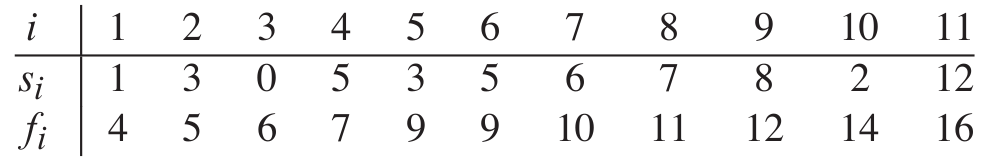
\includegraphics[width=0.7\textwidth]{figs/chap05/activity-example}
\end{figure}
\end{itemize}
\end{frame}

\begin{frame}{‌مسئله انتخاب فعالیت‌ها}
\begin{itemize}\itemr
\item[-]
در مثال زیر این نمونه از مسئله انتخاب فعالیت توسط الگوریتم حریصانه بازگشتی حل شده است.
\begin{figure}
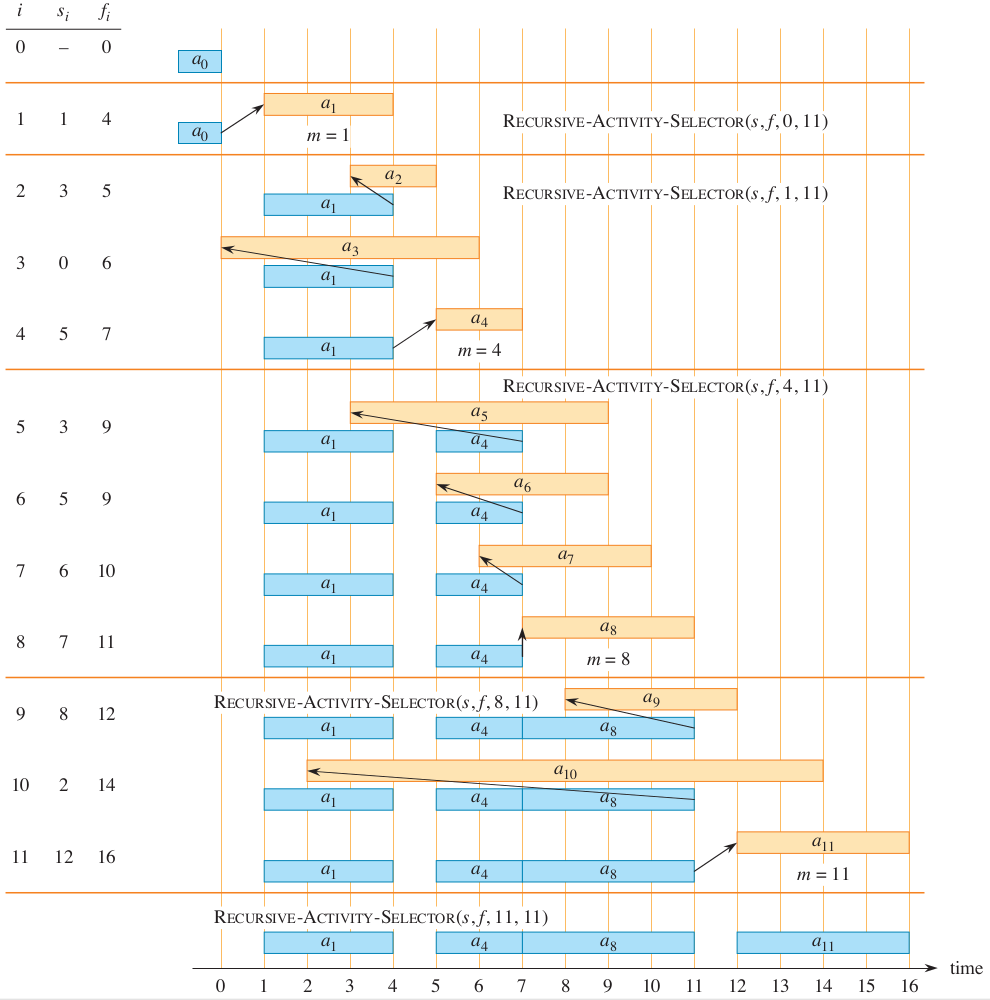
\includegraphics[width=0.47\textwidth]{figs/chap05/activity-recursive-example}
\end{figure}
\end{itemize}
\end{frame}


\iffalse
\begin{frame}{‌مسئله انتخاب فعالیت‌ها}
\begin{itemize}\itemr
\item[-]
این الگوریتم بازگشتی را می‌توانیم به یک الگوریتم غیربازگشتی با یک حلقه تکرار تبدیل کنیم.
\item[-]
به طور کلی همهٔ الگوریتم‌هایی که با یک فراخوانی بازگشتی پایان می‌یابند می‌توانند به الگوریتم‌های غیر بازگشتی با حلقه تکرار تبدیل شوند.
\end{itemize}
\end{frame}
\fi

\begin{frame}{‌مسئله انتخاب فعالیت‌ها}
\begin{itemize}\itemr
\item[-]
الگوریتم زیر مسئله انتخاب فعالیت را به صورت غیر بازگشتی حل می‌کند.
\begin{algorithm}[H]\alglr
  \caption{Greedy-Activity-Selector} 
  \begin{algorithmic}[1]
   \Func{Greedy-Activity-Selector}{s, f, n}
   \State A = \{a[1]\}
   \State k = 1
   \For{m = 2 \To n}
   		\If{s[m] >= f[k]} \LeftComment{is a[m] in S[k] ?}
   				\State A = A $\cup$ \{a[m]\} \LeftComment{yes, so choose it}
   				\State k = m \LeftComment{and continue from there}
   		\EndIf
   	\EndFor
    \State \Return A                       
  \end{algorithmic}
  \label{alg:merge}
\end{algorithm}
\end{itemize}
\end{frame}

\begin{frame}{مسئلهٔ کوله‌پشتی}
\begin{itemize}\itemr
\item[-]
یک الگوریتم حریصانه در هر مرحله انتخابی انجام می‌دهد که در لحظه بهترین انتخاب است و در پایان جواب بهینه نهایی مسئله از این انتخاب‌های بهینه تشکیل شده است. این رویکرد همیشه به جواب بهینه نمی‌رسد اما در برخی مسائل مانند مسئله انتخاب فعالیت جواب بهینه را پیدا می‌کند.
\item[-]
برای حل یک مسئله به روش حریصانه ابتدا ساختار مسئله مشخص می‌شود و یک جواب بازگشتی برای مسئله بر اساس زیر مسئله‌ها طراحی می‌شود. برخلاف روش برنامه‌ریزی پویا که در آن جواب یک مسئله به چند زیرمسئله بستگی پیدا می کند، در مسئله‌هایی که با روش حریصانه حل می‌شوند، جواب یک مسئله به یک زیر مسئله بستگی دارد. پس از یافتن چنین رابطهٔ بازگشتی که در آن جواب یک مسئله تنها به یک زیرمسئله بستگی دارد، یک الگوریتم بازگشتی حریصانه برای مسئله پیدا می‌شود.
%سپس می‌توان الگوریتم بازگشتی را به یک الگوریتم غیر بازگشتی با یک حلقه تکرار تبدیل کرد.
%\item[-]
%به طور خلاصه برای حل یک مسئله به روش حریصانه می‌توان الگوریتمی طراحی کرد که در هر گام یک انتخاب بهینه انجام دهد و تنها یک زیرمسئله برای حل‌کردن باقی می‌ماندو که به طور بازگشتی زیر مسئله‌ها نیز یک انتخاب بهینه صورت می‌دهند. سپس باید اثبات کرد که این روش بهینه را به دست می‌دهد.
\end{itemize}
\end{frame}

\begin{frame}{مسئلهٔ کوله‌پشتی}
\begin{itemize}\itemr
\item[-]
الگوریتم حریصانه مسئله را به صورت از بالا به پایین حل می‌کند، اما برنامه‌ریزی پویا مسئله را از پایین به بالا حل می‌کند.
\item[-]
الگوریتم حریصانه در هر گام انتخابی انجام می‌دهد که بهترین انتخاب است و جواب بهینه از این انتخاب‌های بهینه تشکیل شده است.
\item[-]
در مسئله‌هایی که با الگوریتم حریصانه حل می‌شوند جواب مسئله تنها به جواب یک زیرمسئله بستگی دارد، در حالی که در برنامه‌ریزی پویا، مسئله به چند زیرمسئله بستگی دارد.
\end{itemize}
\end{frame}

\begin{frame}{مسئلهٔ کوله‌پشتی}
\begin{itemize}\itemr
\item[-]
از آنجایی که الگوریتم حریصانه و برنامه‌ریزی پویا شباهت زیادی به یکدیگر دارند و هر دو از زیر مسئله‌های بهینه برای یافتن جواب بهینه مسئله استفاده می‌کنند، ممکن است گاهی برای مسائلی که به روش حریصانه حل می‌شوند، از برنامه‌ریزی پویا استفاده کنیم و یا گاهی به خطا ممکن است بخواهیم مسئله‌ای که به روش برنامه‌ریزی پویا حل می‌شود را به روش حریصانه حل کنیم.
\end{itemize}
\end{frame}


\begin{frame}{مسئلهٔ کوله‌پشتی}
\begin{itemize}\itemr
\item[-]
مسئله کوله پشتی ۱-۰
\fn{1}{\m{0}-\m{1} knapsack problem}
را در نظر بگیرید. یک دزد که مشغول دزدی از یک فروشگاه است، می‌خواهد از بین تعدادی کالا که هر کدام ارزش و وزن مشخصی دارند، تعدادی کالا را در کوله پشتی خود که W کیلوگرم ظرفیت دارد بگذارد، به طوری‌که ارزش کالاهایی که با خود می‌برد حداکثر باشد.
\item[-]
بنابراین این دزد می‌تواند هر زیر مجموعه‌ای از n کالا را بردارد. ارزش کالای i ام برابر است با
\m{v_i}
و وزن آن برابراست با
\m{w_i}
به طوری‌که
\m{v_i}
و
\m{w_i}
دو عدد صحیح هستند. ظرفیت کوله‌پشتی W است و هدف جمع‌آوری تعدادی کالا است که مجموع ارزش آنها حداکثر ممکن باشد.
\item[-]
به این مسئله، مسئله کوله‌پشتی ۱-۰ گفته می‌شود، زیرا دزد به ازای هر کالا باید یا آن را بگذارد یا بردارد و نمی‌تواند قسمتی از کالا را ببرد و قسمتی را بگذارد.
\item[-]
در مسئله کوله پشتی کسری
\fn{2}{fractional knapsack problem}
 دزد می‌تواند یک کالا را به دو قسمت غیر مساوی تقسیم کند و قسمتی از آن را بردارد و قسمتی را با خود ببرد.
\end{itemize}
\end{frame}


\begin{frame}{مسئلهٔ کوله‌پشتی}
\begin{itemize}\itemr
\item[-]
مسئله کوله پشتی ۱-۰ یک مسئلهٔ بهینه‌سازی است که ویژگی آن داشتن زیر ساختار بهینه است، بدین معنی که یک جواب بهینه برای یک مسئله، از جواب بهینه برای زیرمسئله‌های آن تشکیل شده است.
درواقع اگر کالاهای پر ارزش با حداکثر مجموع وزن W را در نظر بگیریم که کالای j را در برگرفته‌اند، آنگاه کالاهای کوله‌پشتی بدون کالای j باید پر ارزش‌ترین کالاها با حداکثر مجموع وزن
\m{W-w_j}
باشند.
\item[-]
همچنین در مسئله کوله‌پشتی کسری، اگر مجموعهٔ پر ارزش‌ترین کالاها با حداکثر وزن W را در نظر بگیریم که مقدار w از کالای j را در برگرفته باشد، آنگاه بقیه کالاهای داخل کوله‌پشتی منهای قسمت w از کالای j با وزن
\m{W-w}
باید پرارزش‌ترین کالاهایی باشند که دزد می‌تواند از بین کالاهای موجود انتخاب کند.
\item[-]
با وجود اینکه این دو مسئله ساختار بسیار مشابهی دارند، روش حریصانه برای مسئله کوله‌پشتی کسری می‌تواند مورد استفاده قرار بگیرد،
در حالی که
 برای مسئله کوله‌پشتی ۱-۰ راه‌حل حریصانه جواب بهینه به دست نمی‌دهد و باید از روش برنامه‌ریزی پویا استفاده کرد.
\end{itemize}
\end{frame}


\begin{frame}{مسئلهٔ کوله‌پشتی}
\begin{itemize}\itemr
\item[-]
برای حل مسئله کوله‌پشتی توسط روش حریصانه، ابتدا ارزش یک کیلوگرم از هر کالا را به صورت
\m{v_i/w_i}
محاسبه می‌کنیم. وقتی ارزش هر کالا مشخص شد، دزد از با ارزش‌ترین کالا شروع می‌کند و سعی می‌کند کوله‌پشتی خود را پر کند. اگر پرارزش‌ترین کالا به اتمام رسید و هنوز کوله‌پشتی فضای خالی داشت، دزد با دومین کالای پرارزش ادامه می‌دهد و سعی می‌کند آنقدر از آن کالا بر دارد تا کوله پشتی پر شود و اگر کوله‌پشتی با کالای پرارزش دوم پر نشد به سراغ کالای پرارزش سوم می‌رود. این روند آنقدر ادامه پیدا می‌کند تا کوله‌پشتی پر شود. این الگوریتم حریصانه نیاز به مرتب‌سازی کالاها بر اساس ارزش آنها در واحد وزن دارد که این کار با استفاده از یک الگوریتم مرتب‌سازی سریع در زمان
\m{O(n \lg n)}
برای 
\m{n}
کالا انجام می‌شود.
\end{itemize}
\end{frame}

\begin{frame}{مسئلهٔ کوله‌پشتی}
\begin{itemize}\itemr
\item[-]
برای اینکه در مسئلهٔ کوله‌پشتی کسری از الگوریتم توصیف شده استفاده کنیم، باید اثبات کنیم الگوریتم درست است.
\item[-]
می‌توانیم درستی این الگوریتم را با استفاده از برهان خلف ثابت کنیم.
فرض کنید کالاهای برداشته شده در کوله‌پشتی بهینه، شامل کالای m که بیشترین چگالی ارزشی
\fn{1}{value density}
 را دارد نشود. به عبارت دیگر کالای m که چگالی ارزشی آن
\m{v_m / w_m}
است به طوری که
\m{\forall i, v_m / w_m > v_i/w_i}
در کوله‌پشتی بهینه نباشد.
دقت کنید که در مسئلهٔ کوله‌پشتی کسری، الزاما کوله‌پشتی پر می‌شود.
\item[-]
بنابراین در کوله‌پشتی کالای k وجود دارد که چگالی ارزشی آن از کالای m کمتر است، یعنی
\m{v_k/w_k < v_m/w_m} .
در اینصورت می‌توانیم x کیلوگرم از کالای k را از کوله‌پشتی برداریم و x کیلوگرم از کالای m را در کوله‌پشتی قرار دهیم.
\item[-]
مقدار
\m{x \cdot (v_m/w_m) - x \cdot (v_k/w_k)}
مثبت است، که با فرض اولیه مبنی بر اینکه کوله‌پشتی بهینه است در تناقض دارد، پس کوله‌پشتی الزاما حاوی کالایی با بیشترین چگالی ارزشی است.
\end{itemize}
\end{frame}


\begin{frame}{مسئلهٔ کوله‌پشتی}
\begin{itemize}\itemr
\item[-]
 الگوریتم حریصانه برای مسئله کوله‌پشتی ۱-۰ نمی‌تواند مورد استفاده قرار بگیرد.
\item[-]
در مسئله کوله‌پشتی ۱-۰ زیر مسئله‌ها باید با یکدیگر مقایسه شوند، در صورتی که جواب بهینه مسئله کوله پشتی کسری تنها به یک زیر مسئله بستگی دارد.
\item[-]
می‌توان با استفاده از یک مثال نقض نشان داد که الگوریتم حریصانه نمی‌تواند در کوله‌پشتی ۱-۰ مورد استفاده قرار بگیرد.
\end{itemize}
\end{frame}


\begin{frame}{مسئلهٔ کوله‌پشتی}
\begin{itemize}\itemr
\item[-]
مثال زیر نشان می‌دهد که روش حریصانه برای مسئله کوله پشتی ۱-۰ الزاما جواب بهینه را به دست نمی‌آورد. با وجود اینکه کالای اول پر ارزش‌ترین کالاست ولی در مسئله کوله پشتی ۱-۰ در جواب بهینه انتخاب نمی‌شود.
 \begin{figure}
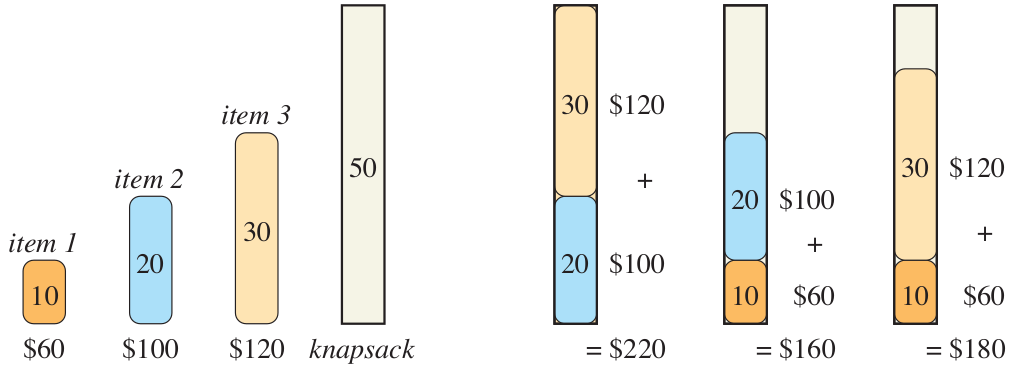
\includegraphics[width=0.7\textwidth]{figs/chap05/knapsack-example}
 \end{figure}
\item[-]
همچنین اگر پر کردن کوله پشتی را با کالاهایی آغاز کنیم که بیشترین قیمت را دارند،
ممکن است کالاها با قیمت بالا حجم زیادی را اشغال کرده و کوله پشتی را پر کنند، در صورتی که مجموع ارزش کالاهای کم ارزش‌تر بیشتر باشد.
\end{itemize}
 \end{frame}


\begin{frame}{مسئلهٔ کوله‌پشتی}
\begin{itemize}\itemr
\item[-]
در مسئله کوله پشتی کسری توسط یک الگوریتم حریصانه شروع به پر کردن کوله پشتی توسط پرارزش‌ترین کالاها می‌کنیم.
\begin{figure}
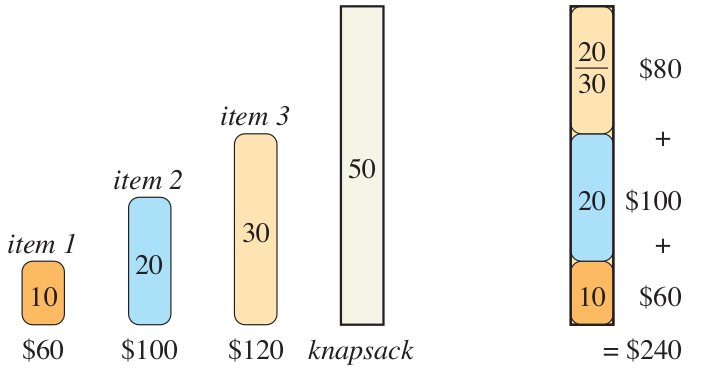
\includegraphics[width=0.6\textwidth]{figs/chap05/knapsack-greedy}
\end{figure}
\end{itemize}
\end{frame}




\begin{frame}{‌کدهای هافمن}
\begin{itemize}\itemr
\item[-]
کدهای هافمن
\fn{1}{Huffman codes}
برای فشرده‌سازی داده‌ها استفاده می‌شوند. این کدها بسته به ویژگی داده‌ها، می‌توانند بین ۲۰ تا ۹۰ درصد در میزان حافظه مورد نیاز برای ذخیره‌سازی داده‌ها صرفه جویی کنند.
\item[-]
 الگوریتم حریصانه هافمن جدولی شامل تعداد تکرار حروف دریافت کرده، سپس برای هر حرف یک کد تولید می‌کند، به طوری که ذخیرهٔ یک متن با استفاده از کدهای تولید شده کمترین میزان حافظه را اشغال کند.
\item[-]
فرض کنید یک فایل داده‌ای داریم که شامل
۱۰۰،۰۰۰
حرف (کاراکتر) است و می‌خواهیم فایل را به صورت فشرده ذخیره کنیم و همچنین می‌دانیم ۶ حرف اول الفبا دارای تعداد تکرارهای ذکر شده در جدول زیر هستند.
\begin{figure}
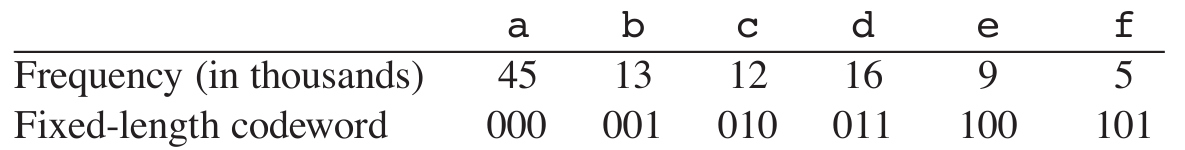
\includegraphics[width=0.7\textwidth]{figs/chap05/huffman-example}
\end{figure}
\end{itemize}
\end{frame}


\begin{frame}{‌کدهای هافمن}
\begin{itemize}\itemr
\item[-]
برای مثال حرف a در این فایل
۴۵،۰۰۰
بار و حرف b تعداد
۱۳،۰۰۰
بار تکرار شده‌اند.
\item[-]
برای نمایش داده‌ها در این فایل راه‌های زیادی وجود دارد. در اینجا از یک کد گذاری دودویی استفاده می‌کنیم. به ازای هر یک از حروف الفبا یک عدد دودویی در نظر گرفته و آن حرف را با کد در نظر گرفته شده نمایش می‌دهیم. به این کدهای دودویی
\fn{1}{binary character  code}
،به اختصار کد می‌گوییم.
\item[-]
می‌توانیم از کدهایی با طول ثابت
\fn{2}{fixed-length code}
استفاده کنیم، که در اینصورت به تعداد
\m{ \lceil \lg n \rceil}
بیت برای نمایش n حرف نیاز داریم. برای ۶ حرف به ۳ بیت نیاز داریم :
\m{a = 000}،
\m{b = 001}،
\m{c = 010}،
\m{d = 011}،
\m{e = 100}و
\m{f = 101}.
\item[-]
با استفاده از این روش کد گذاری برای یک فایل شامل
۱۰۰،۰۰۰
حرف به
۳۰۰،۰۰۰
بیت نیاز داریم. اما آیا می‌توانیم با تعداد کمتری بیت این فایل را ذخیره کنیم؟
\end{itemize}
\end{frame}


\begin{frame}{‌کدهای هافمن}
\begin{itemize}\itemr
\item[-]
برای فشرده‌سازی این فایل متنی و ذخیره‌سازی حروف به طور کارامدتر از کدهایی با طول متغیر
\fn{1}{variable-length code}
استفاده می‌کنیم.
\item[-]
برای نمایش حروفی که تعداد تکرار بیشتری دارند، از کدهای کوتاه‌تر و برای نمایش حروفی که تعداد تکرار کمتری دارند، از کدهای بلندتر استفاده می‌کنیم.
\end{itemize}
\end{frame}


\begin{frame}{‌کدهای هافمن}
\begin{itemize}\itemr
\item[-]
برای مثال یک روش کدگذاری با کدهای طول متغیر در شکل زیر نمایش داده شده است.
\begin{figure}
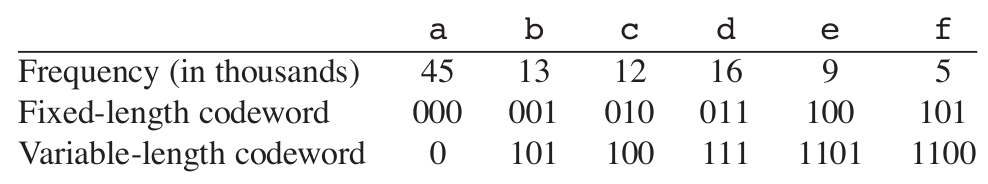
\includegraphics[width=0.7\textwidth]{figs/chap05/huffman-vlc}
\end{figure}
\item[-]
در اینجا از بیت صفر برای نمایش a و عدد چهاربیتی
۱۱۰۰
برای نمایش حروف f استفاده می‌کنیم.
\item[-]
برای نمایش یک فایل شامل
۱۰۰،۰۰۰
حرف با تعداد‌های تکرار ذکر شده به تعداد بیت زیر نیاز داریم‌ :
\begin{align*}
\m{(45 \times 1 + 13 \times 3 + 12 \times 3 + 16 \times 3 + 9 \times 4 + 5 \times 4) \times 1000 = 224000~~\text{bit} }
\end{align*}
\item[-]
بنابراین با استفاده از این روش کدگذاری توانستیم به جای ۳۰۰ هزار بیت از ۲۲۴ هزار بیت استفاده کنیم و حدود ۲۵ درصد در فضای حافظهٔ مورد نیاز صرفه‌جویی کنیم.
\end{itemize}
\end{frame}


\begin{frame}{‌کدهای هافمن}
\begin{itemize}\itemr
\item[-]
در روش کدگذاری استفاده شده، هیچ‌یک از کدها پیشوند کدهای دیگر نبودند. بدین ترتیب به افزودن خط فاصله بین کدها نیازی نداریم و می‌توانیم کدهای یکتا را شناسایی کنیم. به این مجموعهٔ کد، کدهای بدون پیشوند
\fn{1}{prefix-free code}
می‌گوییم.
\item[-]
ثابت شده‌است که کدهای بدون پیشوند بهینه‌ترین روش برای فشرده‌سازی اطلاعات است و هیچ روش کدگذاری بهینه‌تری برای فشرده‌سازی بیشتر وجود ندارد.
\item[-]
با استفاده از روش کدگذاری می‌توانیم کلمهٔ face را به صورت
\begin{align*}
\m{1100 \cdot 0 \cdot 100 \cdot 1101 = 110001001101}
\end{align*}
ذخیره کنیم. در اینجا عملگر
\m{" \cdot "}
به معنی الحاق دو رشته است.
\end{itemize}
\end{frame}


\begin{frame}{‌کدهای هافمن}
\begin{itemize}\itemr
\item[-]
کدهای بدون پیشوند فرایند کدگشایی را ساده می‌کنند. از آنجایی که هیچ کدی پیشوند کد دیگری نیست، کدگذاری یک فایل ابهام ایجاد نمی‌کند. برای کدگشایی یک فایل از ابتدای فایل شروع می‌کنیم و کدها را به ترتیب تبدیل به حروف می‌کنیم.
\item[-]
برای مثال در کدگشایی رشتهٔ
\m{100011001101}
کد
\m{1}
یا
\m{10}
یا
\m{1000}
وجود ندارند و تنها کدی که می‌توان در ابتدای این رشته تشخیص داد، کد
\m{100}
است. این کد معادل کلمه
cafe
می‌باشد.
\begin{align*}
\m{100011001101 = 100 \cdot 0 \cdot 1100 \cdot 1101 = cafe}
\end{align*}
\begin{figure}
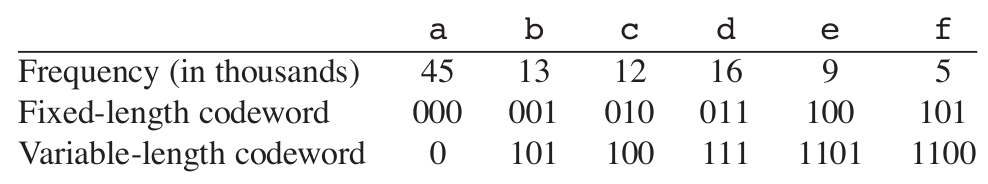
\includegraphics[width=0.7\textwidth]{figs/chap05/huffman-vlc}
\end{figure}
\end{itemize}
\end{frame}


\begin{frame}{‌کدهای هافمن}
\begin{itemize}\itemr
\item[-]
در فرایند کدگشایی برای جستجوی بهینهٔ کدها و حروف متناظر آنها از یک درخت دودویی استفاده می‌کنیم. برگ‌های این درخت دودویی، حروف متناظر با کدهایی هستند که از الحاق کدهای روی یال‌ها از ریشه تا برگ مورد نظر به دست می‌آیند.
\item[-]
به عبارت دیگر کد مربوط به یک حرف درواقع یک مسیر از ریشه تا حرف مورد نظر است به طوری‌که صفر به معنای رفتن به سمت فرزند سمت چپ و یک به معنای رفتن به فرزند سمت راست است.
\end{itemize}
\end{frame}


\begin{frame}{‌کدهای هافمن}
\begin{itemize}\itemr
\item[-]
شکل‌های زیر دو درخت متفاوت برای کدگذاری حروف را نشان می‌دهند.
\begin{figure}
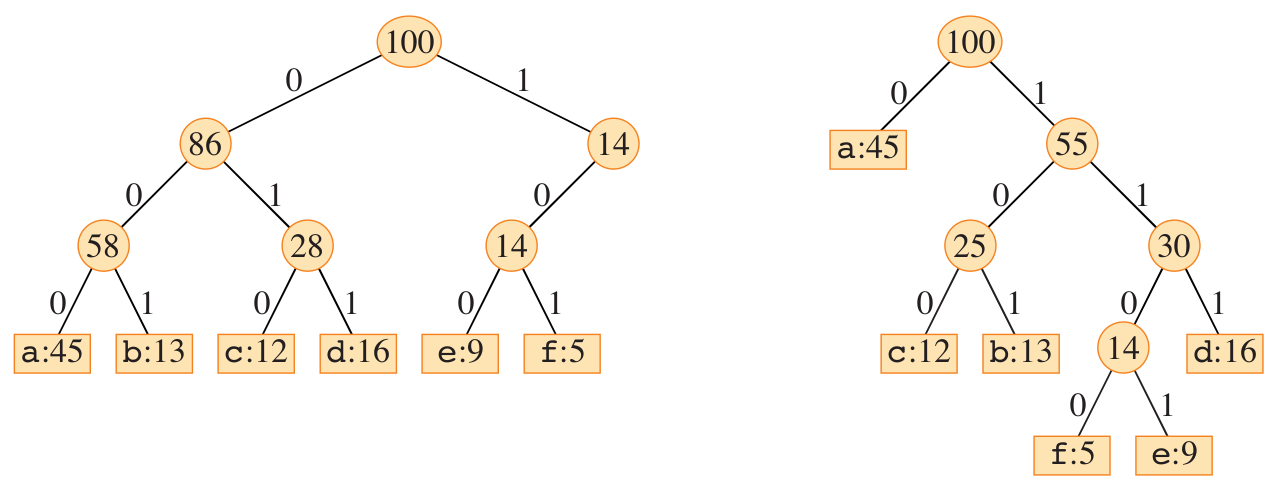
\includegraphics[width=0.9\textwidth]{figs/chap05/huffman-tree}
\end{figure}
\end{itemize}
\end{frame}


\begin{frame}{‌کدهای هافمن}
\begin{itemize}\itemr
\item[-]
می‌توان ثابت کرد که یک کدگذاری بهینه همیشه توسط یک درخت دودویی پُر
\fn{1}{full binary tree}
(درخت اکیدا دودویی)
نشان داده می‌شود،
بدین معنی که هر رأس میانی در درخت بهینه الزاما دارای دو فرزند است. در شکل زیر در سمت چپ، درخت دودویی پر نیست، زیرا به ازای کد ۱۱ هیچ حرفی وجود ندارد،
پس کدگذاری توسط این درخت نمی‌تواند یک کدگذاری بهینه باشد،
 اما درخت سمت راست یک درخت دودویی پر را نشان می‌دهد.
\begin{figure}
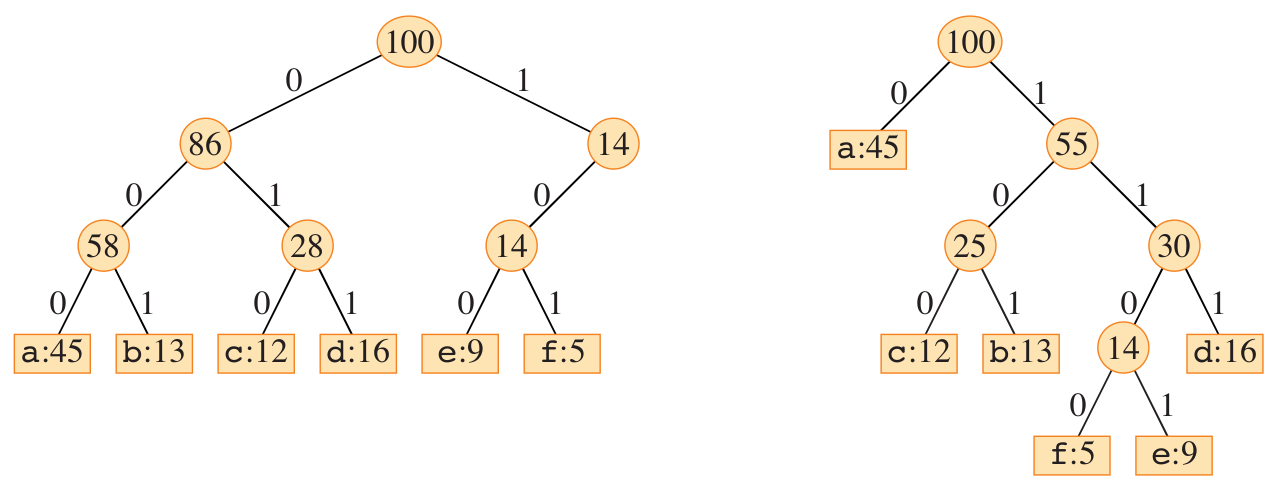
\includegraphics[width=0.6\textwidth]{figs/chap05/huffman-tree}
\end{figure}
%\item[-]
%در درخت سمت چپ از کد ۱ برای هیچ حرفی استفاده نشده است و به همین دلیل این کدگذاری نمی‌تواند بهینه باشد.
\end{itemize}
\end{frame}


\begin{frame}{‌کدهای هافمن}
\begin{itemize}\itemr
\item[-]
یک درخت دودویی پر با 
\m{n}
 برگ الزاما 
\m{n-1}
رأس غیربرگ دارد.
\item[-]
اگر
\m{C}
الفبای مورد نظر برای کدگذاری باشد، درختی که برای کدهای بدون پیشوند بهینه به دست می‌آید، دارای
\m{|C|}
برگ است که هر برگ متناظر با یک حرف است و تعداد
\m{|C| - 1}
رأس میانی (غیربرگ) در درخت داریم.
\end{itemize}
\end{frame}


\begin{frame}{‌کدهای هافمن}
\begin{itemize}\itemr
\item[-]
اگر درخت
\m{T}
درختی برای کدهای بدون پیشوند باشد، می‌توانیم تعداد بیت‌های مورد نیاز برای کدگذاری یک فایل را محاسبه کنیم. به ازای هر حرف c در الفبای
\m{C}
 ، فرض کنید
\m{c.freq}
تعداد تکرار آن حرف در فایل باشد و فرض کنید
\m{d_T(c)}
عمق برگ متناظر با حرف c در درخت باشد. دقت کنید که
\m{d_T(c)}
طول کد متناظر با حرف c نیز هست. در اینصورت تعداد بیت‌های مورد نیاز برای کدگذاری فایل داده‌ای برابراست با
\begin{align*}
\m{B(T) = \sum_{c \in C} c.freq \times d_T(c)}
\end{align*}
\item[-]
به مقدار
\m{B(T)}
هزینه
\fn{1}{cost}
درخت T می‌گوییم.
\end{itemize}
\end{frame}


\begin{frame}{‌کدهای هافمن}
\begin{itemize}\itemr
\item[-]
هافمن یک الگوریتم حریصانه ابداع کرد که کدهای بدون پیشوند بهینه تولید می‌کند. این کدها به کدهای هافمن مشهور هستند.
%\item[-]
%ابتدا الگوریتم حریصانهٔ تولید کدهای هافمن را توضیح می‌دهیم و سپس اثبات می‌کنیم چرا الگوریتم حریصانه در اینجا می‌تواند مورد استفاده قرار بگیرد.
\item[-]
ورودی الگوریتم هافمن مجموعهٔ
\m{C}
شامل n حرف است، به طوری که هر عضو
\m{c \in C}
یک حرف است که ویژگی
\m{c.freq}
تعداد تکرار آن را نشان می‌دهد.
\item[-]
این الگوریتم درخت T را برای تولید کدهای بهینه می‌سازد. این درخت از پایین به بالا تولید می‌شود، بدین معنی که الگوریتم با
\m{|C|}
برگ آغاز می‌کند و با ادغام این برگ‌ها به صورت ساختار درختی، کل درخت را تا ریشه می‌سازد.
\item[-]
در این الگوریتم از یک صف اولویت استفاده می‌شود که حروف با کمترین تعداد‌های تکرار به ترتیب از صف خارج می‌شوند.
\end{itemize}
\end{frame}


\begin{frame}{‌کدهای هافمن}
\begin{itemize}\itemr
\item[-]
الگوریتم هافمن به صورت زیر است.
\begin{algorithm}[H]\alglr
  \caption{Huffman} 
  \begin{algorithmic}[1]
   \Func{Huffman}{C}
   \State n = |C|
   \State Q = C
   \For{i = 1 \To n - 1}
   			\State allocate a new node z
   			\State x = Extract-Min(Q)
   			\State y = Extract-Min(Q)
   			\State z.left = x
   			\State z.right = y
   			\State z.freq = x.freq + y.freq
   			\State Insert(Q,z)
   	\EndFor
   	\State \Return Extract-Min(Q) \LeftComment{the root of the tree is the only node left}                       
  \end{algorithmic}
  \label{alg:merge}
\end{algorithm}
\end{itemize}
\end{frame}


\begin{frame}{‌کدهای هافمن}
\begin{itemize}\itemr
\item[-]
برای مثالی که در قبل مطرح کردیم، الگوریتم هافمن به صورت زیر عمل می‌کند.
\begin{figure}
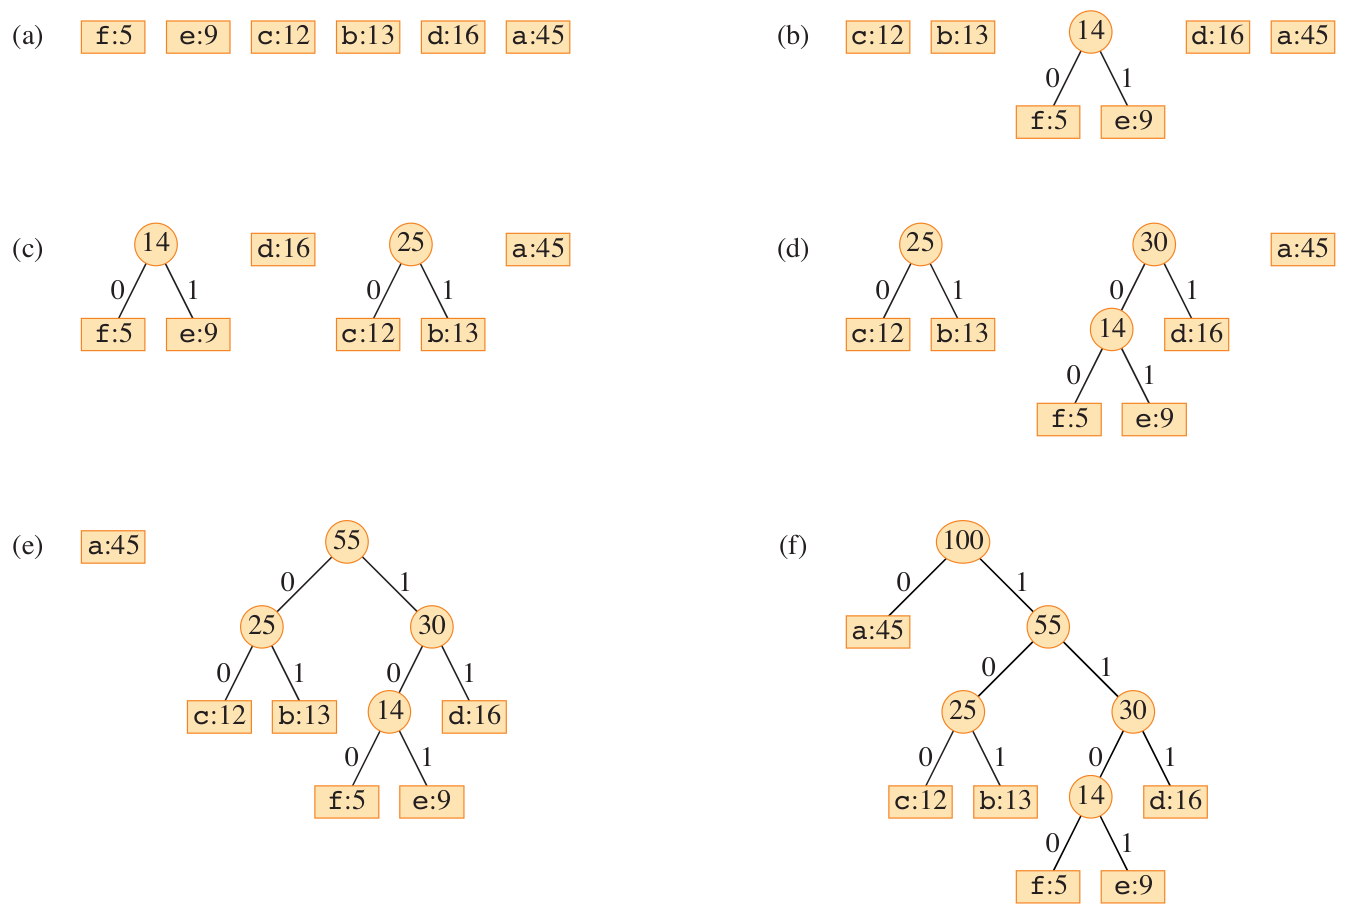
\includegraphics[width=0.7\textwidth]{figs/chap05/huffman-alg-ex}
\end{figure}
\end{itemize}
\end{frame}


\begin{frame}{‌کدهای هافمن}
\begin{itemize}\itemr
\item[-]
زمان الگوریتم هافمن به نحوهٔ پیاده‌سازی صف اولویت بستگی دارد. فرض کنیم با بهینه‌ترین الگوریتم موجود، صف اولویت برای یک الفبا با n حرف در زمان
\m{O(n)}
ساخته می‌شود.
\item[-]
حلقهٔ اصلی در الگوریتم هافمن
\m{n-1}
بار تکرار می‌شود، زیرا تعداد رئوس غیربرگ
\m{n-1}
است
 و از آنجایی که در هر بار استفاده از صف اولویت به زمان
\m{\lg n}
نیاز داریم، بنابراین زمان اجرای الگوریتم
\m{O(n \lg n)}
است.
\item[-]
بنابراین کل زمان اجرای الگوریتم هافمن برای الفبای n حرفی برابراست با
\m{O(n \lg n)}.
\end{itemize}
\end{frame}


\begin{frame}{‌کدهای هافمن}
\begin{itemize}\itemr
\item[-]
برای اثبات اینکه الگوریتم حریصانه هافمن درست است، نشان می‌دهیم مسئله تعیین کدهای بدون پیشوند بهینه دارای ویژگی انتخاب حریصانه است.
\item[-]
به عبارت دیگر می‌خواهیم اثبات کنیم دو رأس با کمترین تعداد تکرار الزاما در درخت کدهای بهینه همزاد یکدیگرند و در بیشترین عمق قرار می‌گیرند.
\end{itemize}
\end{frame}


\begin{frame}{‌کدهای هافمن}
\begin{itemize}\itemr
\item[-]
قضیه : فرض کنید
\m{C}
یک الفبا باشد به طوری‌که
\m{c \in C}
دارای تعداد تکرار
\m{c.freq}
باشد. فرض کنید x و y دو حرف در C با کمترین تعداد‌های تکرار باشند. آنگاه یک کدگذاری بدون پیشوند بهینه برای C وجود دارد به طوری‌که x و y طول یکسانی دارند و تنها در بیت آخر متفات‌اند، یعنی همزاد یکدیگرند و همچنین در بیشترین عمق درخت قرار دارند.
\end{itemize}
\end{frame}


\begin{frame}{‌کدهای هافمن}
\begin{itemize}\itemr
\item[-]
اثبات : ایدهٔ اثبات این است که درخت
\m{T}
که یک درخت بهینهٔ بدون پیشوند را در نظر بگیریم و آن را تغییر دهیم تا یک درخت دودویی بدون پیشوند دیگر ساخته شود به طوری‌که در درخت ساخته شده x و y همزاد
\fn{1}{sibiling}
و در عمق بیشینه در درخت
\m{T}
باشند. چنین درختی که در آن x و y همزاد یکدیگرند یعنی طول یکسان دارند و تنها در بیت آخر متفاوت‌اند، نیز یک درخت بهینه خواهد بود.
\item[-]
فرض کنید a و b دو حرف باشند که در درخت
\m{T}
همزاد هستند و در بیشترین عمق درخت قرار دارند. حال فرض کنید
\m{a.freq \leqslant b.freq}
و
\m{x.freq \leqslant y.freq}.
از آنجایی‌که
\m{x.freq}
و
\m{y.freq}
کمترین تعداد‌های تکرار هستند و
\m{a.freq}
و
\m{b.freq}
دو تعداد تکرار دلخواه هستند، بنابراین خواهیم داشت
\m{x.freq \leqslant a.freq}
و
\m{y.freq \leqslant b.freq}.
\item[-]
بنابراین می‌توانیم داشته باشیم
\m{x.freq = a.freq}
و
\m{y.freq = b.freq}
که در اینصورت قضیه به طور بدیهی درست است، زیرا a و b دارای کمترین تعداد تکرار هستند.
 پس فرض می‌کنیم تعداد تکرارهای
 x 
 و
 y
 متفاوت از a و b هستند.
\end{itemize}
\end{frame}


\begin{frame}{‌کدهای هافمن}
\begin{itemize}\itemr
\item[-]
همانطور که شکل زیر نشان می‌دهد، فرض کنید جای a و x را در درخت
\m{T}
عوض می‌کنیم و درخت
\m{T'}
را به‌دست می‌آوریم و جای b و y را در درخت 
\m{T'}
عوض کرده،
درخت
\m{T''}
را به دست می‌آوریم.
\begin{figure}
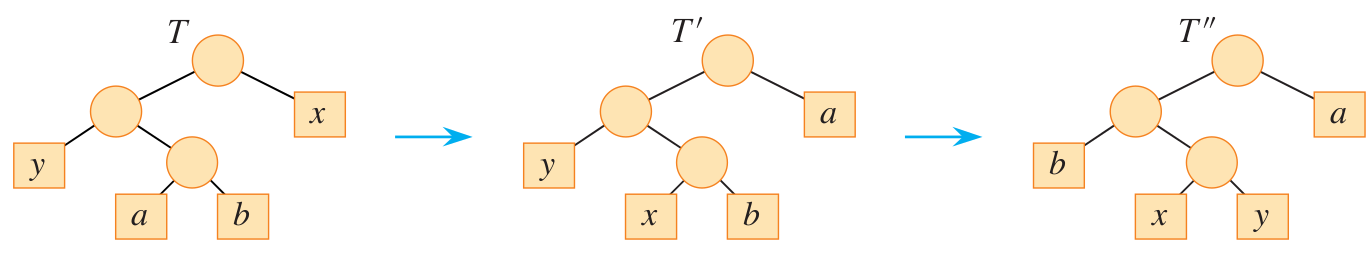
\includegraphics[width=0.9\textwidth]{figs/chap05/huffman-proof}
\end{figure}
\item[-]
نشان می‌دهیم که هزینهٔ درخت
\m{T''}
کوچکتر یا مساوی درخت
\m{T}
 است.
 از آنجایی که فرض کردیم درخت 
 \m{T}
 یک درخت بهینه است، بنابراین هزینه درخت 
 \m{T''}
 و
\m{T}
باید برابر باشد.
\end{itemize}
\end{frame}


\begin{frame}{‌کدهای هافمن}
\begin{itemize}\itemr
\item[-]
تفاوت هزینهٔ درخت
\m{T}
و
\m{T'}
به صورت زیر خواهد بود.
\begin{align*}
\m{B(T)} & \m{- B(T')}\\
&\m{= \sum_{c \in C} c.freq \cdot d_T(c) - \sum_{c \in C} c.freq \cdot d_{T'}(c)}\\
&\m{= x.freq \cdot d_T(x) + a.freq \cdot d_T(a) - x.freq \cdot d_{T'}(x) - a.freq \cdot d_{T'}(a)}\\
&\m{= x.freq \cdot d_T(x) + a.freq \cdot d_T(a) - x.freq \cdot d_T(a) - a.freq \cdot d_T(x)}\\
&\m{= (a.freq - x.freq) (d_T(a) - d_T(x))}\\
&\m{\geqslant 0}
\end{align*}
\end{itemize}
\end{frame}


\begin{frame}{‌کدهای هافمن}
\begin{itemize}\itemr
\item[-]
از آنجایی که
\m{a.freq - x.freq}
و همچنین
\m{d_T(a) - d_T(x)}
غیر منفی هستند، بنابراین مقدار
\m{B(T) - B(T')}
مثبت است.
\item[-]
درواقع
\m{a.freq - x.freq}
غیر منفی است زیرا x یک برگ با حداقل تعداد تکرار است و
\m{d_T(a) - d_T(x)}
غیر منفی است زیرا a یک برگ با عمق بیشینه در درخت
\m{T}
است.
\item[-]
به همین ترتیب تعویض y و b هزینه را افزایش نمی‌دهد و بنابراین
\m{B(T') - B(T'')}
نیز غیر منفی است.
\item[-]
بنابراین
\m{B(T'') \leqslant B(T') \leqslant B(T)}
و چون
\m{T}
بهینه است بنابراین داریم
\m{B(T) \leqslant B(T'')}
و بنابراین
\m{B(T'') = B(T)}
در نتیجه
\m{T''}
یک درخت بهینه است که در آن x و y دو برگ همزاد با عمق حداکثر هستند و قضیه ثابت می‌شود.
\end{itemize}
\end{frame}


\begin{frame}{‌کدهای هافمن}
\begin{itemize}\itemr
\item[-]
این قضیه در واقع نشان می‌دهد که ساختن درخت بهینه، می‌تواند با انتخاب حریصانه ادغام دو حرف با کمترین تعداد تکرار آغاز شود و ادامه یابد. بنابراین از بین همهٔ انتخاب‌ها برای ادغام الگوریتم هافمن دو حرف با کمترین تعداد را در هر مرحله انتخاب می‌کند که یک انتخاب بهینه است، و همچنین درخت کلی به دست آمده در نهایت یک درخت بهینه خوهد بود.
\end{itemize}
\end{frame}


\begin{frame}{‌کدهای هافمن}
\begin{itemize}\itemr
\item[-]
حال می‌خواهیم ثابت کنیم ساختن کدهای بدون پیشوند بهینه دارای ویژگی زیر ساختار بهینه است.
\item[-]
به عبارت دیگر، می‌خواهیم اثبات کنیم اگر رأس z به عنوان پدر رئوس x و y با کمترین تعداد تکرار به همراه بقیه رئوس درخت به جز x و y ، یک درخت کدهای بهینه را تشکیل دهند، آنگاه درختی که در آن x و y به عنوان فرزندان z اضافه شده‌اند نیز درخت کدهای بهینه است.
\end{itemize}
\end{frame}


\begin{frame}{‌کدهای هافمن}
\begin{itemize}\itemr
\item[-]
قضیه : فرض کنید
\m{C}
یک الفبا باشد به طوری‌که برای هر حرف
\m{c \in C}
تعداد تکرار c برابر با
\m{c.freq}
باشد. فرض کنید x و y دو حرف در
\m{C}
با تعداد تکرار حداقل باشند. فرض کنید
\m{C'}
همان الفبای 
\m{C}
 باشد به طوری‌که حروف x و y حذف شده و حرف z به آن اضافه شده است، بنابراین
\m{C' = (C - \{x,y\}) \cup \{z\}}
تعداد تکرار همهٔ حروف در
\m{C'}
برابر با حروف
\m{C}
هستند و همچنین
\m{z.freq = x.freq + y.freq}.
فرض کنید
\m{T'}
درختی باشد که کدهای بدون پیشوند بهینه
\m{C'}
را نمایش می‌دهد. آنگاه درخت
\m{T}
که از درخت
\m{T'}
به دست آمده و در آن رأس z با یک رأس میانی با دو فرزند x و y به جایگزین شده است، کدهای بدون پیشوند بهینه برای الفبای
\m{C}
را نمایش می‌دهد.
\end{itemize}
\end{frame}


\begin{frame}{‌کدهای هافمن}
\begin{itemize}\itemr
\item[-]
اثبات : ابتدا نشان می‌دهیم چگونه هزینه
\m{B(T)}
از درخت
\m{T}
بر اساس هزینهٔ
\m{B(T')}
از درخت
\m{T'}
بیان می‌شود.
\item[-]
به ازای هر حرف
\m{c \in C - \{x,y\}}
، داریم
\m{d_T(c) = d_{T'}(c)}
و بنابراین
\m{c.freq \times d_T(c) = c.freq \times d_{T'}(c)} .
\item[-]
چون
\m{d_T(x) = d_T(y) = d_{T'}(z) + 1}
،بنابراین داریم :
\begin{align*}
\m{x.freq \times d_T(x) + y.fraq \times d_T(y)} & \m{= (x.freq + y.freq)(d_{T'}(z) + 1)}\\
& \m{= z.freq \times d_{T'}(z) + (x.freq + y.freq)}
\end{align*}
\item[-]
بنابراین نتیجه می‌گیریم
\m{B(T) = B(T') + x.freq + y.freq}
که برابر است با
\m{B(T') = B(T) - x.freq - y.freq}.
\item[-]
حال از برهان خلف استفاده می‌کنیم.
\end{itemize}
\end{frame}


\begin{frame}{‌کدهای هافمن}
\begin{itemize}\itemr
\item[-]
فرض کنید
\m{T}
درخت بهینه بدون پیشوند برای
\m{C}
نیست. بنابراین یک درخت
\m{T''}
بهینه وجود دارد به طوری‌که
\m{B(T'') < B(T)}.
درخت
\m{T''}
دو رأس x و y را به عنوان همزاد درخود دارد.
\item[-]
حال فرض کنید
\m{T'''}
همان درخت
\m{T''}
باشد که در آن پدر مشترک x و y با رأس برگ z جایگزین شده است به طوری‌که
\m{z.freq = x.freq + y.freq}
\item[-]
بنابراین :
\begin{align*}
\m{B(T''')} & \m{= B(T'') - x.freq - y.freq}\\
& \m{< B(T) - x.freq - y.freq}\\
& \m{= B(T')}
\end{align*}
\item[-]
به این نتیجه رسیدیم که 
\m{T'''}
یک درخت بهینه برای 
\m{C'}
است، اما با این نتیجه 
 به تناقض می‌رسیم زیرا فرض کردیم
\m{T'}
درخت بدون پیشوند بهینه برای
\m{C'}
است. بنابراین
\m{T}
باید کدهای بدون پیشوند بهینه برای الفبای
\m{C}
را نمایش دهد.
\end{itemize}
\end{frame}


\begin{frame}{‌کدهای هافمن}
\begin{itemize}\itemr
\item[-]
دو قضیهٔ اثبات شده نشان می‌دهند الگوریتم هافمن کدهای بدون پیشوند بهینه تولید می‌کند.
\end{itemize}
\end{frame}


%%%%%%%%%%%%%%%%%%%%%%%%%
\section{جستجوی ترکیبیاتی}
%%%%%%%%%%%%%%%%%%%%%%%%%

\begin{frame}{‌جستجوی ترکیبیاتی}
\begin{itemize}\itemr
\item[-]
روش‌های تقسیم و حل، برنامه‌ریزی پویا و حریصانه را برای حل دسته‌ای از مسئله‌های محاسباتی بررسی کردیم. در مسئله‌های بررسی شده، یک راه‌حل ساده برای پیدا کردن جواب مسئله جستجوی همهٔ حالت‌ها است ولی چنین جستجویی در زمان معقول (زمان چند جمله‌ای) امکان پذیر نیست چرا که تعداد همهٔ حالت‌های ممکن از مرتبه نمایی است و بنابراین جستجوی همهٔ حالت‌ها در زمان نمایی صورت می‌گیرد. توسط روش‌های تقسیم و حل، برنامه‌ریزی پویا و حریصانه روش‌هایی برای حل مسئله‌ها در زمان معقول ارائه کردیم.
\item[-]
پیدا کردن جواب در زمان چند جمله‌ای برای همهٔ مسئله‌ها همیشه امکان پذیر نیست و گاهی تنها راه حل ، جستجوی فضای حالت برای آن مسئله است. جستجوی فضای حالت به معنی تولید همهٔ جواب‌های مسئله و انتخاب حالت بهینه یا حالت مورد نظر از بین همهٔ حالت‌های ممکن است. تعداد این حالت‌ها از مرتبهٔ نمایی است و بنابراین چنین الگوریتم‌هایی به زمان نمایی برای محاسبه نیاز دارند و در نتیجه برای مسائلی با اندازهٔ بزرگ در عمل قابل استفاده نیستند.
\end{itemize}
\end{frame}


\begin{frame}{‌جستجوی ترکیبیاتی}
\begin{itemize}\itemr
\item[-]
در مبحث جستجوی ترکیبیاتی
\fn{1}{combinatorial search}
، روش‌های جستجوی همه فضای حالت برای یک مسئله بررسی می‌شود. در این روش‌ها مطالعه می‌کنیم چگونه به طور منظم همهٔ حالت‌ها را بررسی کنیم و یا اینکه چگونه با استفاده از روش‌هایی فضای حالت را محدود کنیم.
\item[-]
ترکیبیات
\fn{2}{combinatorics}
شاخه‌ای از ریاضیات است که در آن به بررسی ساختارهای متناهی و شمارش این ساختارها می‌پردازیم.
\item[-]
برای مثال گراف یک ساختار متناهی است و تعداد مسیرها در یک گراف، متناهی است. برای پیدا کردن بلندترین مسیر در یک گراف می‌توانیم همهٔ مسیرها را بررسی و بلندترین آنها را انتخاب کنیم.
\item[-]
بهینه سازی ترکیبیاتی
\fn{3}{combinatorial optimization}
شاخه‌ای از بهینه‌سازی است که در آن مجموعهٔ جواب‌های امکان پذیر گسسته است و هدف پیدا کردن جواب بهینه از بین همهٔ جواب‌های ممکن است.
\end{itemize}
\end{frame}

\begin{frame}{‌پسگرد}
\begin{itemize}\itemr
\item[-]
روش پسگرد
\fn{1}{backtrack}
روشی است که با استفاده از آن همهٔ فضای حالت را جستجو می‌کنیم. در این روش با یکی از حالت‌ها در فضای حالت شروع می‌کنیم و برای انتخاب حالت بعد یکی از پارامترهای فضای حالت را تغییر می‌دهیم. ممکن است در انتخاب حالت بعد، چند پارامتر قابل تغییر باشند. در اینصورت یکی از پارامترها را تغییر می‌دهیم و به حالت بعد می‌رویم و سپس پسگرد می‌کنیم تا یکی دیگر از پارامترها را تغییر دهیم. بدین صورت همهٔ حالت‌ها در فضای حالت بررسی می‌شوند.
\end{itemize}
\end{frame}

\iffalse
\begin{frame}{‌پسگرد}
\begin{itemize}\itemr
\item[-]
برای مثال فرض کنید می‌خواهیم همهٔ رشته‌ها با طول ۲ که از سه حرف a و b و c تشکیل شده‌اند را بشماریم. یا به عبارت دیگر همهٔ فضای حالت را تولید کنیم.
\item[-]
با استفاده از روش پسگرد در ابتدا ۳ انتخاب برای حرف اول داریم حرف a را انتخاب می‌کنیم و سپس از بین ۳ انتخاب برای حرف دوم، حرف a را انتخاب می‌کنیم پس رشتهٔ aa را به دست می‌آوریم، سپس پسگرد می‌کنیم و حرف b را برای حرف دوم رشته انتخاب می‌کنیم و رشته ab را بدست می‌آوریم. بار دیگر با یک پسگرد رشتهٔ ac را بدست می‌آوریم. در پسگرد بعدی هیچ انتخابی برای حرف دوم وجود نخواهد داشت پس دوباره پسگرد می‌کنیم و حرف b را به عنوان حرف اول انتخاب می‌کنیم. با استفاده از این روش به ترتیب رشته‌های
ba
،
bb
،
bc
،
ca
،
cb
و
cc
به دست می‌آیند.
\end{itemize}
\end{frame}
\fi

\begin{frame}{‌پسگرد}
\begin{itemize}\itemr
\item[-]
فرض کنید وارد یک باغ پر پیچ و خم یا باغ هزارتو
\fn{1}{maze}
شده‌اید و می‌خواهید راه خروجی را پیدا کند. راه را در پیش می‌گیرید و به هر چند راهی که می‌رسید راه اول از سمت چپ را انتخاب می‌کنید. در پایان یا راه خروجی را پیدا می‌کنید و یا به بن‌بست بر می‌خورید. در صورتی که به بن‌بست رسیدید، بازمی‌گردید تا به اولین چندراهی قبل از بن‌بست برسید. به جای راه اول از سمت چپ، دومین راه از سمت چپ را امتحان می‌کنید و در صورت برخورد با بن‌بست راه را باز می‌گردید و در چند راهی راه سوم را امتحان می‌کنید. فرض کنید که همهٔ راه‌ها در چند راهی آخر را امتحان کردید و به بن‌بست خوردید. در این صورت باید مسیر را بازگردید تا به دومین چند راهی قبل از بن‌بست برسید و این بار در دومین چندراهی قبل از بن‌بست، دومین راه را انتخاب کنید. این روند را ادامه می‌دهید تا راه خروجی را پیدا کنید. به این روش حل مسئله روش پسگرد گفته می‌شود.
\item[-]
هر یک از چندراهی‌ها یکی از پارامترهای مسئله است که مقادیر مختلف آن را امتحان می‌کنید.
\end{itemize}
\end{frame}


\begin{frame}{‌پسگرد}
\begin{itemize}\itemr
\item[-]
روش پسگرد وقتی استفاده می‌شود که می‌خواهیم مسئله‌ای را حل کنیم که در آن عناصر یک دنباله
\fn{1}{sequence}
باید از اشیائی از یک مجموعهٔ
\fn{2}{set}
معین انتخاب شوند، به طوری‌که دنباله ویژگی مشخصی داشته باشد و معیار
\fn{3}{criterion}
معینی را برآورده کند.
\end{itemize}
\end{frame}

\begin{frame}{مسئلهٔ چند وزیر}
\begin{itemize}\itemr
\item[-]
می‌خواهیم تعداد n وزیر را در یک صفحه شطرنج
\m{n \times n}
به گونه‌ای قرار دهیم که هیچ یک از وزیرها همدیگر را تهدید نکنند. به عبارت دیگر هیچ دو وزیری نباید در یک سطر یا ستون یا خط مورب مشترکی قرار بگیرند.
\item[-]
دنباله‌ای که در این مسئله به دنبال آن می‌گردیم، دنباله‌ای است از n مکان که n وزیر در آنها قرار گرفته‌اند. مجموعه‌ای که هر یک از عناصر دنباله می‌توانند از  اعضای آن مجموعه انتخاب شوند عبارت است از مجموعه‌ای شامل
\m{n^2}
مکان بر روی صفحهٔ شطرنج.
\item[-]
ویژگی معینی که این دنباله باید داشته باشد این است که هیچ دو مکان انتخاب شده‌ای بر روی یک خط افقی، عمودی یا مورب قرار نگیرد.
\item[-]
مسئلهٔ چند وزیر یا
n
وزیر،
 حالت کلی مسئلهٔ ۸ وزیر است که در آن ۸ وزیر در یک صفحه شطرنج استاندارد با تعداد
۸ $\times$ ۸
مکان قرار می‌گیرند.
\item[-]
در اینجا برای سهولت نمایش حالات مختلف مسئله ۴ وزیر را در نظر می‌گیریم.
\end{itemize}
\end{frame}


\begin{frame}{مسئلهٔ چند وزیر}
\begin{itemize}\itemr
\item[-]
روش پسگرد در واقع روشی است که در یک درخت
\fn{1}{tree}
به صورت عمق-اول
\fn{2}{depth-first}
جستجو می‌کند. پس ابتدا جستجوی عمق-اول در درخت را توضیح می‌دهیم.
\item[-]
فرض کنید درختی داریم که از تعدادی رأس و یال تشکیل شده است و می‌خواهیم همهٔ مسیرهای درخت را که با ریشه شروع می‌شوند و با یک برگ پایان می‌یابند بررسی کنیم.
\item[-]
در واقع دنباله‌هایی که در اینجا بررسی می‌کنیم دنباله‌هایی هستند که یک مسیر در درخت را نشان می‌دهند و با ریشه آغاز و با یکی از برگ‌ها پایان می‌یابند.
\end{itemize}
\end{frame}


\begin{frame}{مسئلهٔ چند وزیر}
\begin{itemize}\itemr
\item[-]
ابتدا به سراغ ریشهٔ درخت می‌رویم و ریشه را به عنوان اولین عنصر دنباله انتخاب می‌کنیم. سپس اولین فرزند از سمت چپ در سطح یک درخت را انتخاب می‌کنیم و اگر این رأس دارای فرزند بود اولین فرزند آن را در سطح دو انتخاب می‌کنیم. این کار را ادامه می‌دهیم تا به یک برگ برسیم. تا اینجا یک مسیر در درخت را بررسی کرده‌ایم. با فرض اینکه برگ در سطح n قرار دارد، به رأس پدر در سطح
\m{n-1}
باز می‌گردیم و فرزند دوم را انتخاب می‌کنیم. این کار را ادامه می‌دهیم تا مسیر دوم و به همین ترتیب همهٔ مسیرها در درخت را بررسی کنیم.
\end{itemize}
\end{frame}


\begin{frame}{مسئلهٔ چند وزیر}
\begin{itemize}\itemr
\item[-]
درخت زیر را در نظر بگیرید. با استفاده از روش پسگرد ابتدا مسیر
\m{(1,2,3)}
سپس
\m{(1,2,4,5)}
سپس
\m{(1,2,4,6)}
، و به همین ترتیب
\m{(1,2,7)}
،
\m{(1,8,9)}
،
\m{(1,8,10)}
، الی آخر بررسی می‌شوند.
\begin{figure}
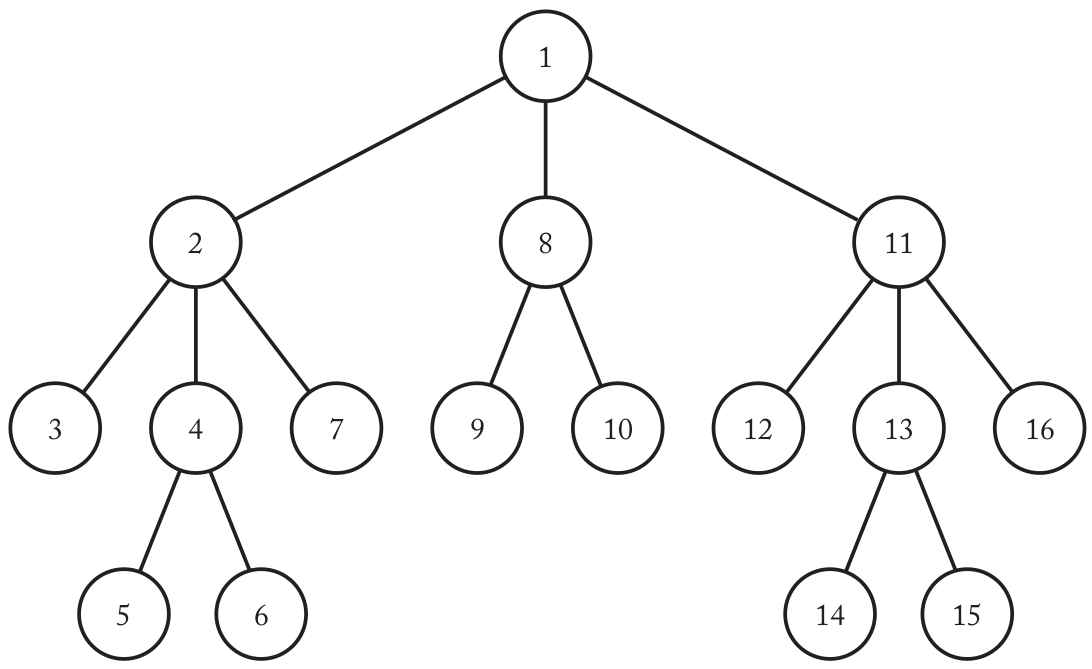
\includegraphics[width=0.6\textwidth]{figs/chap06/tree-backtrack}
\end{figure}
\end{itemize}
\end{frame}


\begin{frame}{مسئلهٔ چند وزیر}
\begin{itemize}\itemr
\item[-]
الگوریتم زیر این روش پسگرد را نشان می‌دهد.
\begin{algorithm}[H]\alglr
  \caption{Depth First TreeSearch} 
  \begin{algorithmic}[1]
   \Func{Depth-First-Tree-Search}{node v}
	 \State visit(v)
	 \For{each child u of v}
   			\State Depth-First-Tree-Search(u)
   	 \EndFor                     
  \end{algorithmic}
  \label{alg:merge}
\end{algorithm}
\end{itemize}
\end{frame}


\begin{frame}{مسئلهٔ چند وزیر}
\begin{itemize}\itemr
\item[-]
حال که با روش پسگرد آشنا شدیم، مسئلهٔ ۴ وزیر را در نظر می‌گیریم. می‌خواهیم ۴ وزیر را در یک صفحهٔ شطرنج
۴ $\times$ ۴
به گونه‌ای قرار دهیم که هیچ دو وزیری یکدیگر را تهدید نکنند. از آنجایی که هیچ دو وزیری نمی‌توانند در یک سطر قرار بگیرند، پس هر وزیر را باید در یک سطر متفاوت از بقیه وزیرها قرار دهیم. از آنجایی که هر وزیر در هر یک از ستون‌ها می تواند قرار بگیرد، بنابراین تعداد همهٔ حالت‌هایی که باید بررسی شوند برابر است با
۲۵۶ = ۴ $\times$ ۴ $\times$ ۴ $\times$ ۴.
\item[-]
برای بررسی همهٔ حالت‌ها درختی تشکیل می‌دهیم که در آن،
مکان اولین وزیر در سطح یک انتخاب می‌شود و مکان وزیر دوم در سطح دوم و به همین ترتیب مکان وزیر سوم در سطح سوم و مکان وزیر چهارم در سطح چهارم انتخاب می‌شوند.
\item[-]
یک مسیر از ریشه تا برگ درواقع یکی از گزینه‌های انتخاب مکان‌های صفحه را نشان می‌دهد. یک گزینه جواب مسئله است اگر در آن هیچ دو وزیری یکدیگر را تهدید نکنند.
\item[-]
به درخت تشکیل شده درخت فضای حالت گفته می‌شود.
\end{itemize}
\end{frame}


\begin{frame}{مسئلهٔ چند وزیر}
\begin{itemize}\itemr
\item[-]
قسمتی از درخت فضای حالات مسئله ۴ وزیر در شکل زیر نمایش داده شده است.
\begin{figure}
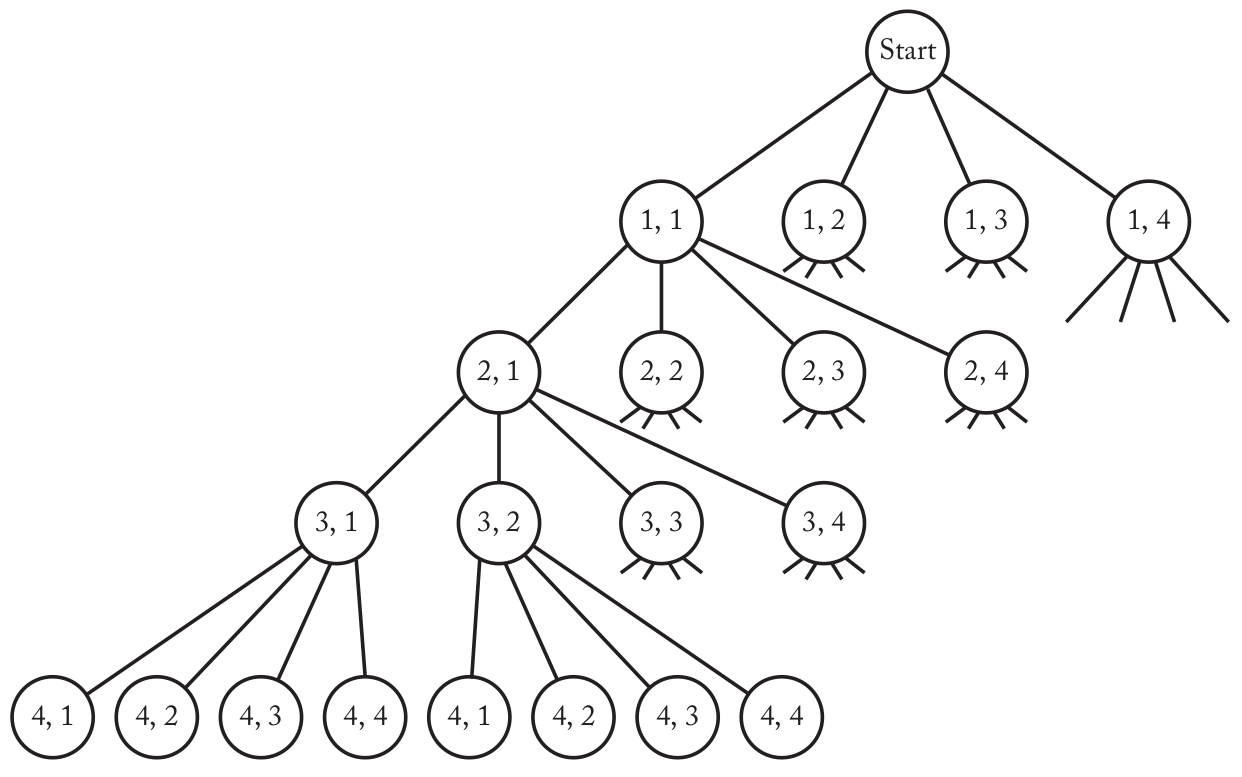
\includegraphics[width=0.7\textwidth]{figs/chap06/n-queens-tree}
\end{figure}
\end{itemize}
\end{frame}


\begin{frame}{مسئلهٔ چند وزیر}
\begin{itemize}\itemr
\item[-]
این درخت در مجموع ۲۵۶ برگ دارد که هر مسیر از ریشه تا یکی از برگ‌ها یکی از گزینه‌ها را نشان می‌دهد. در هریک از رأس‌های درخت یک جفت
\m{(i,j)}
ذخیره می‌شود که برابر با یک مکان در صفحهٔ شطرنج در سطر i و ستون j است.
\end{itemize}
\end{frame}


\begin{frame}{مسئلهٔ چند وزیر}
\begin{itemize}\itemr
\item[-]
 جستجو در این درخت می تواند بهینه‌تر از بررسی همهٔ ۲۵۶ انتخاب نیز انجام شود. برای مثال وقتی وزیر اول در مکان
\m{(1,1)}
قرار گرفت، بدیهی است که وزیر دوم نمی‌تواند در مکان
\m{(2,1)}
قرار بگیرد پس این مسیر در درخت ادامه داده نمی‌شود. همینطور وزیر دوم نمی‌تواند در مکان دوم قرار بگیرد پس نیازی نداریم این مسیر را نیز ادامه دهیم.
\item[-]
در شکل زیر این بهینه‌سازی نشان داده شده است.
\begin{figure}
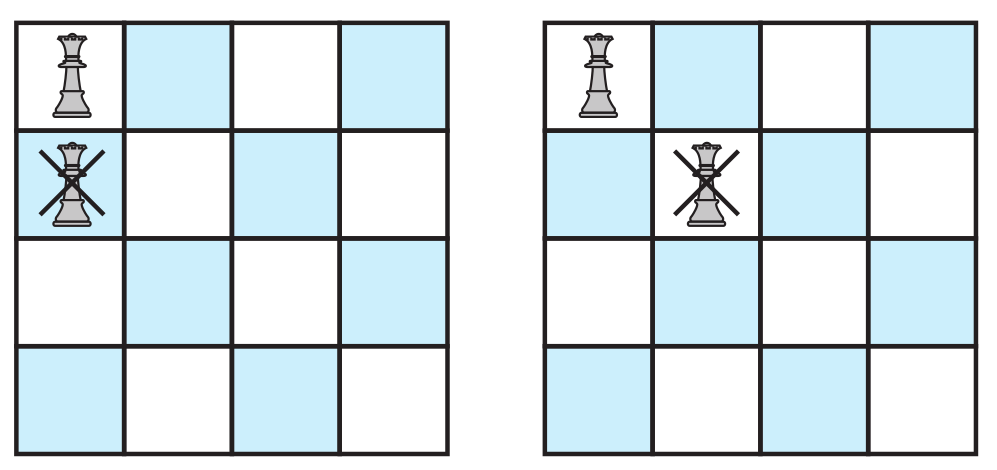
\includegraphics[width=0.6\textwidth]{figs/chap06/n-queens-opt}
\end{figure}
\end{itemize}
\end{frame}


\begin{frame}{مسئلهٔ چند وزیر}
\begin{itemize}\itemr
\item[-]
پسگرد عبارت است از روندی که توسط آن وقتی در یک انتخاب به یک گزینهٔ غیر جواب می‌رسیم، در درخت فضای حالت به عقب بازمی‌گردیم یا به عبارت دیگر از انتخاب یک رأس صرف نظر می‌کنیم و به رأس پدر پسگرد می‌کنیم تا فرزند بعدی پدر را انتخاب کنیم.
\item[-]
به یک رأس در درخت فضای حالت نومید کننده
\fn{1}{nonpromising}
می‌گوییم، اگر انتخاب آن رأس به جواب نیانجامد و به همین ترتیب به یک رأس امید دهنده
\fn{2}{promising}
می‌گوییم اگر با انتخاب آن همچنان احتمال رسیدن به جواب وجود داشته باشد.
\end{itemize}
\end{frame}


\begin{frame}{مسئلهٔ چند وزیر}
\begin{itemize}\itemr
\item[-]
به طور خلاصه در روش پسگرد، بر روی درخت فضای حالت، جستجوی عمق اول انجام می‌دهیم و در فرایند جستجو اگر به رأس نومید کننده برخورد کردیم مسیر را ادامه نمی‌دهیم و به رأس پدر پسگرد می‌کنیم.
\item[-]
به این روش هرس‌کردن
\fn{1}{pruning}
فضای حالت نیز گفته می‌شود که در آن تعدادی از دنباله‌ها بررسی نمی‌شوند.
\end{itemize}
\end{frame}


\begin{frame}{مسئلهٔ چند وزیر}
\begin{itemize}\itemr
\item[-]
در حالت کلی این الگوریتم به صورت زیر نوشته می‌شود.
\begin{algorithm}[H]\alglr
  \caption{Checknode} 
  \begin{algorithmic}[1]
   \Func{Checknode}{node v}
   \If{promising(v)}
   		\If{there is a solution at v}
   				\State write the solution
   		\Else
   			\For{each child u of v}
   					\State Checknode(u)
   			\EndFor
   		\EndIf
   	\EndIf                           
  \end{algorithmic}
  \label{alg:merge}
\end{algorithm}
\end{itemize}
\end{frame}


\begin{frame}{مسئلهٔ چند وزیر}
\begin{itemize}\itemr
\item[-]
ریشهٔ فضای حالت به تابع
Checknode
داده می‌شود که توسط آن رأس ریشه بررسی می‌شود. در بررسی یک رأس، ابتدا باید بررسی شود که انتخاب آن رأس امید دهنده است یا نومید کننده. اگر انتخاب آن امید دهنده بود و به جواب رسیدیم،‌ جواب را چاپ می‌کنیم. اگر انتخاب امید دهنده بود ولی به جواب نرسیدیم، رئوس فرزند به ترتیب برای بررسی انتخاب می‌شود.
\end{itemize}
\end{frame}


\begin{frame}{مسئلهٔ چند وزیر}
\begin{itemize}\itemr
\item[-]
تابع
promising
برای مسئله‌های مختلف متفاوت است. در مسئلهٔ ۴ وزیر، این تابع مقدار نادرست باز می‌گرداند اگر مکان‌های انتخاب شده از ریشه تا رأس مورد بررسی، به صورت سطری، ستونی یا قطری در یک راستا باشند.
\end{itemize}
\end{frame}


\begin{frame}{مسئلهٔ چند وزیر}
\begin{itemize}\itemr
\item[-]
در شکل زیر قسمتی از درخت فضای حالت به صورت هرس شده نشان‌داده شده است.
\begin{figure}
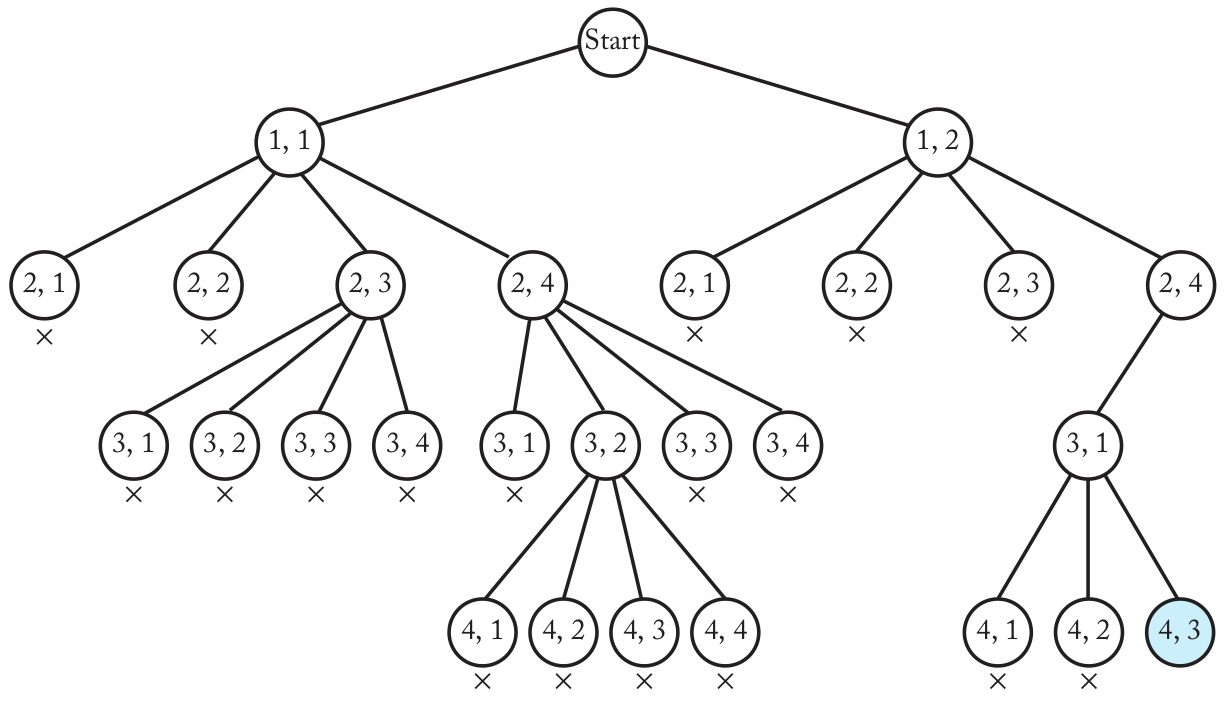
\includegraphics[width=0.7\textwidth]{figs/chap06/n-queens-tree2}
\end{figure}
\end{itemize}
\end{frame}


\begin{frame}{مسئلهٔ چند وزیر}
\begin{itemize}\itemr
\item[-]
در شکل زیر روند بررسی فضای حالت در صفحهٔ شطرنج نشان‌داده شده است.
\begin{figure}
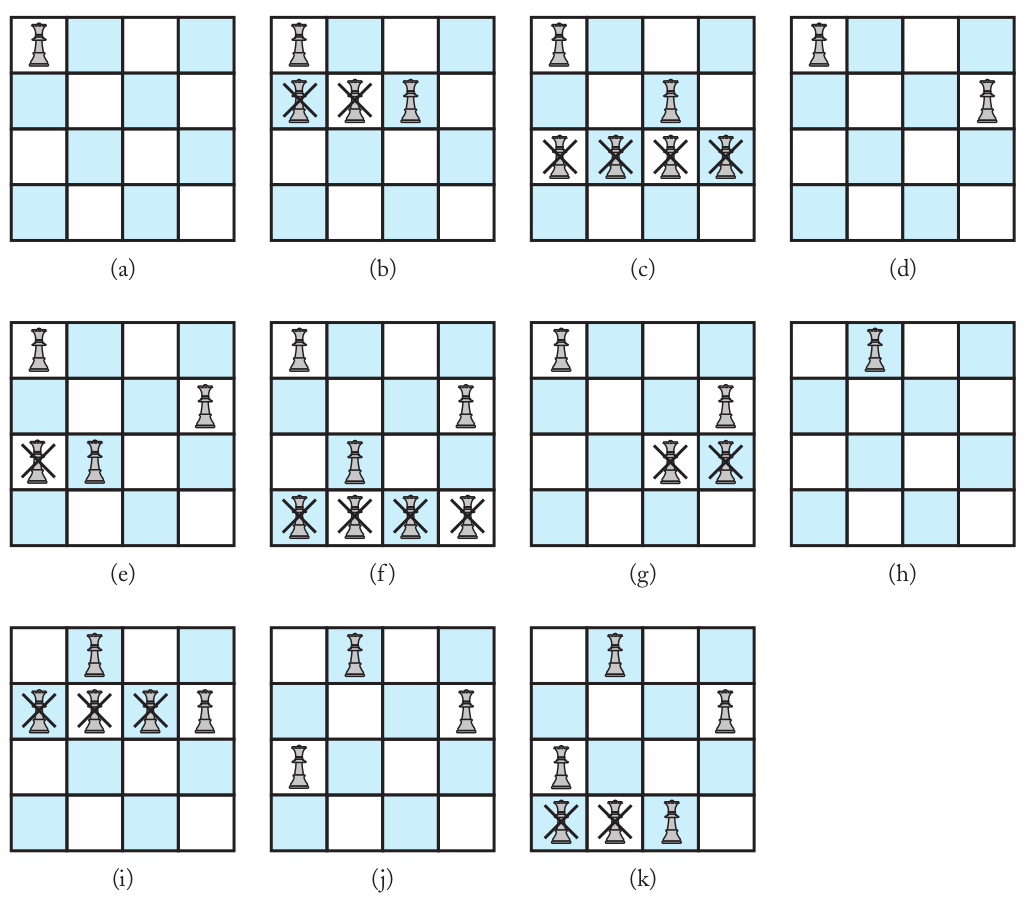
\includegraphics[width=0.5\textwidth]{figs/chap06/n-queens-board}
\end{figure}
\end{itemize}
\end{frame}


\begin{frame}{مسئلهٔ چند وزیر}
\begin{itemize}\itemr
\item[-]
تابع
promising
باید بررسی کند که آیا دو وزیر در یک ستون یا قطر قرار گرفته‌اند یا خیر.
\item[-]
اگر
\m{col(i)}
ستونی باشد که وزیر i ام در آن قرار گرفته است، باید بررسی کنیم که
\m{col(i)}
و
\m{col(j)}
برای هیچ دو وزیر i و j برابر نباشد.
\item[-]
همچنین دو وزیر به صورت مورب یکدیگر را تهدید می‌کنند اگر
\m{col(i) - col(j) = i - j}
و یا
\m{col(i) - col(j) = j - i}
باشد.
\end{itemize}
\end{frame}


\begin{frame}{مسئلهٔ چند وزیر}
\begin{itemize}\itemr
\item[-]
الگوریتم پسگرد برای مسئلهٔ چند وزیر به صورت زیر است. برای شروع الگوریتم تابع
\code{Queens(0)}
فراخوانی می‌شود.
\begin{algorithm}[H]\alglr
  \caption{Queens} 
  \begin{algorithmic}[1]
   \Func{Queens}{index i}
   \If{Promising(i)}
   		\If{i == n}
   				\State print col[1] through col[n]
   		\Else
   		\Statex \LeftComment{See if queen in (i+1)-st row can be}
   		\Statex \LeftComment{positioned in each of the n columns.}
   				\For{j = 1 \To n}
   					\State col[i + 1] = j
   					\State Queens(i + 1)	
   				\EndFor
   		\EndIf
  \EndIf                       
  \end{algorithmic}
  \label{alg:merge}
\end{algorithm}
\end{itemize}
\end{frame}


\begin{frame}{مسئلهٔ چند وزیر}
\begin{itemize}\itemr
\item[-]
\begin{algorithm}[H]\alglr
  \caption{Promising} 
  \begin{algorithmic}[1]
   \Func{Promising}{index i}
   \Statex  \LeftComment{Check if any queen k threatens queen in the i-th row.}	
   \For{k = 1 \To i - 1}	 
   			\If{col[i] == col[k] \textbf{or} |col[i] − col[k]| == i − k}
   					\State \Return false
   			\EndIf
   	\EndFor
   	\State \Return true                  
  \end{algorithmic}
  \label{alg:merge}
\end{algorithm}
\end{itemize}
\end{frame}


\begin{frame}{مسئلهٔ چند وزیر}
\begin{itemize}\itemr
\item[-]
حال می‌خواهیم الگوریتم پسگرد برای چند وزیر را تحلیل کنیم.
برای این کار تعداد رئوسی که در درخت فضای حالت بررسی می‌شوند را محاسبه می‌کنیم. از آنجایی که به دست آوردن تعداد دقیق حالات  وقتی حالت‌ها هرس می‌شوند ساده نیست، برای تعداد رئوس بررسی شده در درخت فضای حالت یک کران بالا در نظر می‌گیریم.
\item[-]
در درخت فضای حالات در سطح صفر، یک رأس داریم، در سطح یک تعداد n رأس، در سطح ۲ تعداد
\m{n^2}
رأس و در سطح n تعداد
\m{n^n}
رأس داریم. پس تعداد همهٔ رئوس بررسی شده برابر است با :
\begin{align*}
\m{1 + n + n^2 + n^3 + \cdots + n^n = \frac{n^{n+1} - 1}{n-1}}
\end{align*}
\item[-]
برای مسئله ۸ وزیر این تعداد برابر است با
\begin{align*}
\m{\frac{8^{8+1}-1}{8-1} = 19,173,961}
\end{align*}
\end{itemize}
\end{frame}


\begin{frame}{مسئلهٔ چند وزیر}
\begin{itemize}\itemr
\item[-]
حال یک کران بالای دیگر برای تعداد رئوس بررسی شده در نظر می‌گیریم. می‌دانیم که هیچ دو وزیری نمی‌توانند در یک ستون قرار بگیرند، بنابراین وقتی وزیر اول انتخاب شد، وزیر دوم تنها در ۷ مکان می‌تواند قرار بگیرد پس در سطح اول ۸ رأس و در سطح دوم
\LR{۸ $\times$ ۷}
رأس، در سطح سوم
\LR{۸ $\times$ ۷ $\times$ ۶}
رأس داریم و بدین ترتیب الی آخر.
\item[-]
پس در حالت کلی کران بالای رئوس بررسی شده برابراست با :
\begin{align*}
\m{1 + n + n(n-1) + n(n-1)(n-2) + \cdots + n!}
\end{align*}
\item[-]
برای مسئله ۸ وزیر این تعداد برابراست با
۱۰۹،۶۰۱
رأس.
\end{itemize}
\end{frame}


\begin{frame}{مسئلهٔ چند وزیر}
\begin{itemize}\itemr
\item[-]
تعداد دقیق رئوس بررسی شده را می‌توانیم با پیاده‌سازی الگوریتم به دست آوریم.
\item[-]
از آنجایی که کران بالای تعداد حالت مورد بررسی
\m{n!}
است، زمان اجرای الگوریتم پسگرد برای مسئلهٔ n وزیر
\m{O(n!)}
است.
\end{itemize}
\end{frame}
\iffalse
\begin{frame}{شاخه و کران}
\begin{itemize}\itemr
\item[-]
روش شاخه و کران
\fn{1}{branch and bound}
برای بهبود الگوریتم‌های پسگرد به کار می‌روند.
\item[-]
روش شاخه و کران، همچون روش پسگرد درخت فضای حالت را برای یافتن جواب بررسی می‌کند.
\item[-]
یک الگوریتم شاخه و کران در هر رأس درخت جستجوی حالات،
کرانی را محاسبه می‌کند که با استفاده از مقدار کران می‌توان گفت آیا آن رأس
 امید دهنده است یا خیر. مقداری که به عنوان کران در هر رأس محاسبه می‌شود، با استفاده از کرانی بر روی جواب مسئله به دست می‌آید.
\end{itemize}
\end{frame}
\fi

\begin{frame}{شاخه و کران}
\begin{itemize}\itemr
\item[-]
روش شاخه و کران
\fn{1}{branch and bound}
 همچون روش پسگرد درخت فضای حالت را برای یافتن جواب بررسی می‌کند.
\item[-]
این روش معمولاً برای مسائل بهینه‌سازی استفاده می‌شود. در مسائل بهینه‌سازی هدف یافتن جواب بهینه (کوچکترین، بزرگترین، ...) است. در هر لحظه در هنگام پیمایش درخت فضای حالت یکی از جواب‌های به دست آمده تا آن لحظه بهینه است. بنابراین قبل از بسط دادن یک رأس می‌توانیم محاسبه کنیم آیا جوابی که با بسط دادن آن رأس به دست می‌آید، از جواب بهینه‌ای که تا آن لحظه به دست آمده است، بهتر است یا خیر. در صورتی که امیدی به یافتن جواب بهتر نبود، رأس مورد پیمایش بسط داده نمی‌شود.
\item[-]
بنابراین اگر با بسط دادن یک رأس امید به یافتن جواب بهینه‌تر وجود نداشت، می‌گوییم آن رأس نومیدکننده
\fn{2}{nonpromising}
است، در غیر اینصورت امیددهنده
\fn{3}{promising}
است.
یک الگوریتم شاخه و کران در هر رأس درخت جستجوی حالات،
کرانی را محاسبه می‌کند که با استفاده از مقدار کران می‌توان گفت آیا آن رأس
 امید دهنده است یا خیر.
\end{itemize}
\end{frame}


\begin{frame}{شاخه و کران}
\begin{itemize}\itemr
\item[-]
می‌توانیم مسئلهٔ کوله پشتی ۱-۰ را با استفاده از روش پسگرد حل کنیم.
\item[-]
در سطح اول در درخت فضای حالت، دو حالت بررسی می‌شوند : (۱) کالای اول در کوله پشتی قرار می‌گیرد، یا (۲) کالای اول در کوله‌پشتی قرار نمی‌گیرد. همینطور در سطح دوم به ازای هر یک از دو حالت سطح اول درخت، باید دو حالت بررسی شوند : اینکه کالای دوم در کوله‌پشتی قرار می‌گیرد یا نمی‌گیرد.
این فرایند ادامه پیدا می‌کند تا به یک جواب برسیم و هزینه کوله‌پشتی را محاسبه کنیم. در یک الگوریتم پسگرد باید همهٔ برگ‌های درخت فضای حالت بررسی شده، برگی که بیشترین هزینه را دارد انتخاب شود. 
\end{itemize}
\end{frame}

\begin{frame}{شاخه و کران}
\begin{itemize}\itemr
\item[-]
همچنین در حل این مسئله
 می‌توان از روش شاخه و کران استفاده کرد. برای بررسی اینکه
 یک رأس امیددهنده است یا خیر،
باید محاسبه کنیم که آیا حداکثر ارزشی که می‌تواند با برداشتن باقی اشیاء حاصل شود، از جواب بهینهٔ به دست آمده تا آن لحظه بیشتر است یا خیر.
تنها در صورتی بسط یک رأس را ادامه می‌دهیم که امیدی به بهبود جواب داشته باشیم.
\item[-]
یک الگوریتم شاخه و کران به ازای هر رأس در درخت فضای حالت محاسبه می‌کند آیا هزینه‌ای که با بسط آن رأس به دست می‌آید از جواب بهینه به دست آمده بهتر خواهد بود یا خیر. به عبارت دیگر می‌گوییم در هر رأس یک کران محاسبه می‌شود و با استفاده از کران محاسبه شده تصمیم گرفته می‌شود رأس مورد بررسی هرس شود یا خیر.
%\item[-]
%در هر لحظه در حین اجرای الگوریتم پسگرد، یکی از جواب های به دست آمده جواب بهینه است. در هر رأس درخت فضای حالت برای اجناس باقیمانده خارج از کوله پشتی یک کران بالا با استفاده از الگوریتم حریصانه (با فرض این که اجناس را می‌توان تقسیم کرد) به دست می‌آوریم. اگر مقدار این کران بالا از جواب بهینه به دست آمده تا آن لحظه کمتر بود، آن رأس را بسط نمی‌دهیم زیرا امیدی به پیدا کردن جواب بهینه با بسط آن رأس وجود نخواهد داشت.
\end{itemize}
\end{frame}

\begin{frame}{شاخه و کران}
\begin{itemize}\itemr
\item[-]
در روش شاخه و کران، با استفاده از مقدار کران به دست آمده، نه تنها می‌توان تصمیم گرفت که یک رأس بسط داده شود و یا خیر، بلکه می‌توان علاوه بر آن با استفاده از کران به دست آمده، تصمیم گرفت کدام رأس برای بسط دادن مناسب‌تر است.
\item[-]
با استفاده از این روش معمولاً می‌توان با سرعت بیشتری به جواب بهینه دست پیدا کرد.
\item[-]
به این روش جستجوی بهتر اول
\fn{1}{best-first search}
با هرس کردن شاخه و کران
\fn{2}{branch and bound pruning}
گفته می‌شود.
\end{itemize}
\end{frame}


\begin{frame}{شاخه و کران}
\begin{itemize}\itemr
\item[-]
در جستجوی بهتر اول، درخت فضای حالت را با استفاده از جستجوی سطح اول
\fn{1}{breadth-first search}
 پیمایش می‌کنیم.
%در جستجوی درخت فضای حالت گاهی به جای جستجوی عمق اول، از جستجوی سطح اول
%\fn{1}{breadth-first search}
%استفاده می‌شود.
\item[-]
در پیمایش سطح اول، ابتدا ریشه بررسی می‌شود، سپس رئوس سطح یک و پس از آن رئوس سطح دو و بدین ترتیب همهٔ رئوس تا برگ‌ها بررسی می‌شوند.
\item[-]
برخلاف جستجوی عمق اول که در آن از یک الگوریتم بازگشتی استفاده می‌شود، در جستجوی سطح-اول از یک صف برای پیمایش رئوس درخت استفاده می‌کنیم.
\item[-]
بدین ترتیب فرزندان یک رأس در صف قرار می‌گیرند و به ترتیب فرزندان یک به یک از صف خارج شده و فرزندانشان پیمایش می‌شوند. بنابراین در این روش ابتدا سطح اول درخت، سپس سطح دوم و به همین ترتیب همهٔ سطوح پیمایش می‌شوند. به همین دلیل به این جستجو سطح-اول گفته می‌شود.
\end{itemize}
\end{frame}


\begin{frame}{شاخه و کران}
\begin{itemize}\itemr
\item[-]
الگوریتم زیر الگوریتم جستجوی درخت با استفاده از روش سطح-اول را نشان می‌دهد.
\begin{algorithm}[H]\alglr
  \caption{Breadth-First-Tree-Search} 
  \begin{algorithmic}[1]
   \Func{Breadth-First-Tree-Search}{tree T}
   \State queue Q
   \State node u, v
   \State initialize(Q)		\LeftComment{initialize Q to be empty.}
   \State u = root(T)
   \State visit(u)
   \State enqueue(Q, u)
   \While{!empty(Q)}
   		\State v = dequeue(Q)
   		\For{each child u of v}
   				\State visit(u)
   				\State enqueue(Q, u)
   		\EndFor
   \EndWhile                        
  \end{algorithmic}
  \label{alg:merge}
\end{algorithm}
\end{itemize}
\end{frame}

\begin{frame}{مسئلهٔ فروشندهٔ دوره‌گرد}
\begin{itemize}\itemr
\item[-]
یک فروشندهٔ دوره‌گرد می‌خواهد برای فروش اجناس خود به همهٔ شهرها سفر کند.
هر دو شهر می‌توانند توسط یک جادهٔ یک طرفه به یکدیگر متصل شده باشند و هر جاده طولی معین دارد.
فروشندهٔ دوره‌گرد می‌خواهد از شهر خود سفر را آغاز کند و مسیری را بپیماید که از هر شهر تنها یک بار عبور کند و در پایان به شهر خود بازگردد.
در ضمن می‌خواهد مسیر پیموده شده کوتاهترین مسیر باشد.
\item[-]
این مسئله را با استفاده از یک گراف مدلسازی می‌کنیم.
در یک گراف جهت‌دار، می‌خواهیم کوتاه‌ترین مسیری را پیدا کنیم که از یک رأس آغاز می‌شود، از هریک از رئوس تنها یک بار عبور می‌کند و به رأس اول باز می‌گردد. چنین مسیری یک مسیر بهینه است. از آنجایی که این مسیر بهینه از همهٔ رئوس عبور می‌کند، بنابراین می‌توانیم از هر رأسی مسیر را آغاز کنیم. به مسیری که از هر رأس تنها یک بار عبور می‌کند مسیر همیلتونی می‌گوییم و به مسیری که از هر رأس تنها یک بار عبور کند و به رأس اول بازگردد یک دور همیلتونی می‌گویند. در اینجا به دنبال کوتاهترین دور همیلتونی می‌گردیم.
\end{itemize}
\end{frame}


\begin{frame}{مسئلهٔ فروشندهٔ دوره‌گرد}
\begin{itemize}\itemr
\item[-]
در شکل زیر ماتریس مجاورت برای یک گراف جهت‌دار نشان داده شده است که در آن از هر رأس به رأس دیگر یک یال وجود دارد. اعداد در ماتریس مجاورت طول یال‌ها از یک رأس به رأس دیگرند. کوتاهترین دور همیلتونی در این گراف نشان داده شده است.
\begin{figure}
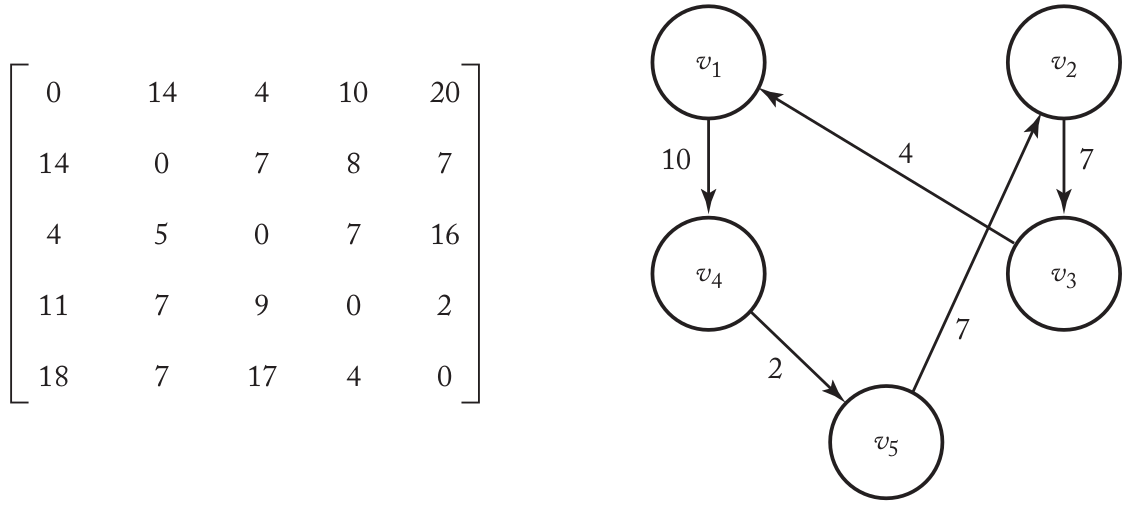
\includegraphics[width=0.7\textwidth]{figs/chap06/263-tsp}
\end{figure}
\end{itemize}
\end{frame}


\begin{frame}{مسئلهٔ فروشندهٔ دوره‌گرد}
\begin{itemize}\itemr
\item[-]
قسمتی از درخت جستجوی فضای حالت برای این مسئله در زیر نشان داده شده است.
\begin{figure}
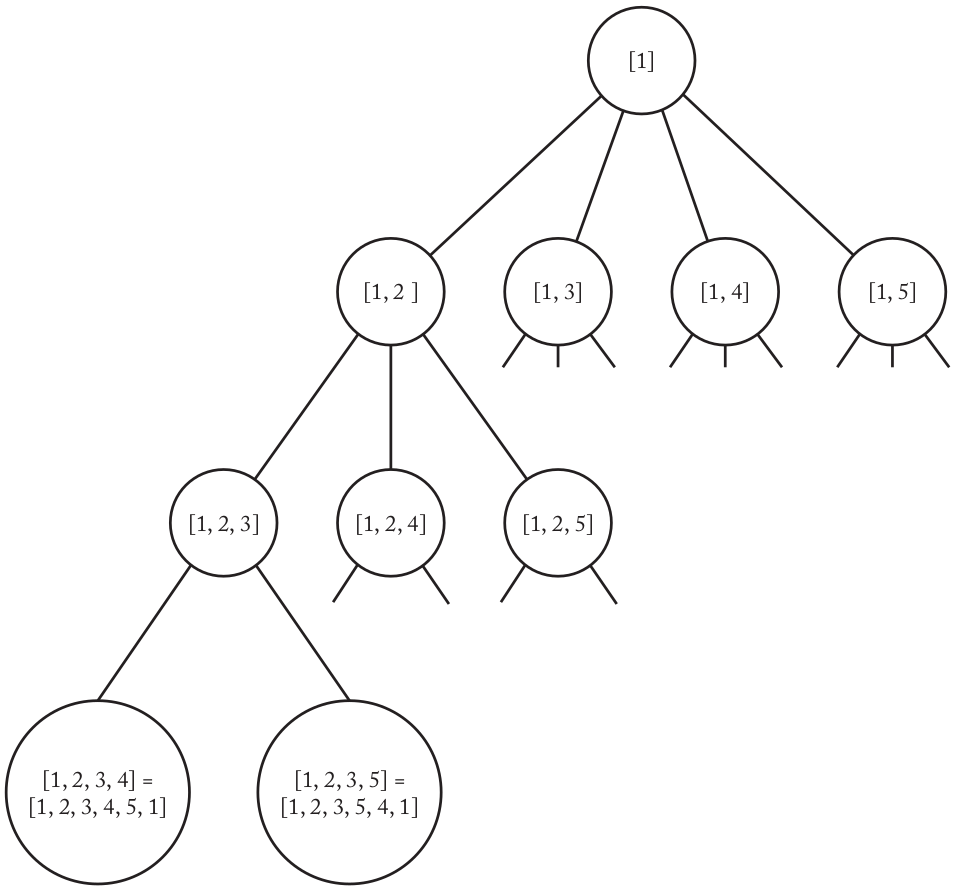
\includegraphics[width=0.5\textwidth]{figs/chap06/264-tsp}
\end{figure}
\end{itemize}
\end{frame}


\begin{frame}{مسئلهٔ فروشندهٔ دوره‌گرد}
\begin{itemize}\itemr
\item[-]
در این درخت فضای حالت، با رأس شماره ۱ از گراف آغاز می‌کنیم. مسیر بهینه ممکن است از هر یک از رئوس ۲ ، ۳ ، ۴ و ۵ عبور کند، بنابراین به ازای هریک از این رئوس یک فرزند در سطح یک در درخت فضای حالت می‌سازیم. رأس
\m{[1,2]}
در درخت فضای حالت مسیری را در گراف مشخص می‌کند که از رأس ۱ و ۲ در گراف عبور کند.
\end{itemize}
\end{frame}


\begin{frame}{مسئلهٔ فروشندهٔ دوره‌گرد}
\begin{itemize}\itemr
\item[-]
اکنون باید برای هر رأس در درخت فضای حالت یک مقدار کران پیدا کنیم. در هر رأس درخت فضای حالت یک کران پایین برای طول مسیری که می‌توان با بسط دادن آن رأس به دست آورد محاسبه می‌کنیم.
\item[-]
اگر کران پایین محاسبه شده در یک رأس از کوتاهترین مسیر همیلتونی به دست آمده تا آن لحظه کمتر باشد، آن رأس درخت فضای حالت امیددهنده است و آن رأس را بسط می‌دهیم، در غیر اینصورت آن رأس نومیدکننده است و بسط دادن را از آن رأس ادامه نمی‌دهیم.
\end{itemize}
\end{frame}


\begin{frame}{مسئلهٔ فروشندهٔ دوره‌گرد}
\begin{itemize}\itemr
\item[-]
برای محاسبهٔ کران به صورت زیر عمل می‌کنیم.
\item[-]
در هر رأس درخت فضای حالت تعدادی از رئوس گراف پیمایش شده و تعدادی پیمایش نشده‌اند.
به ازای رأس‌های پیمایش شده در گراف طول مسیر معین شده است. اما به ازای رأس‌های پیمایش نشده در گراف باید یک کران پایین برای طول مسیر محاسبه کنیم.
\item[-]
رأس پیمایش نشدهٔ
\m{V_i}
را در نظر بگیرید. جهت پیدا کردن یک کران پایین برای کوتاهترین مسیر،
به ازای هریک از رأس‌های پیمایش نشدهٔ
\m{V_i}
باید کوتاهترین یال خروجی از آن رأس را به صورت
\m{\min_{k} (V_i,V_k)}
 محاسبه کنیم و طول کوتاهترین یال‌های خروجی را به ازای همهٔ رئوس پیمایش نشده به صورت
\m{\sum_{i} \min_{k} (V_i,V_k)}
محاسبه کنیم.
\item[-]
 به عبارت دیگر به ازای هر یک از رئوس پیمایش نشدهٔ
\m{V_i}
باید یالی را پیدا کنیم که از
\m{V_i}
خارج می‌شود و کمترین هزینه را دارد.
مجموع طول این یال‌ها یک کران پایین برای طول مسیر است.
توجه کنید که این بدین معنا نیست که کوتاهترین‌ها الزاما در مسیر همیلتونی انتخاب می‌شوند، بلکه بدین معناست که هیچ مسیر همیلتونی با طول کمتر از مقدار محاسبه شده وجود نخواهد داشت.
\end{itemize}
\end{frame} 


\begin{frame}{مسئلهٔ فروشندهٔ دوره‌گرد}
\begin{itemize}\itemr
\item[-]
محاسبه کران را با یک مثال بررسی می‌کنیم. ماتریس مجاورت زیر را در نظر بگیرید.
\begin{figure}
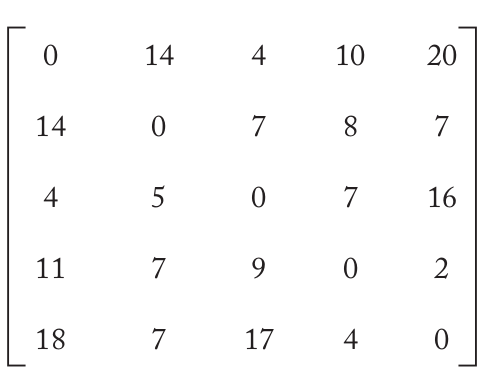
\includegraphics[width=0.2\textwidth]{figs/chap06/263-tsp-matrix}
\end{figure}
\item[-]
در ریشه درخت فضای حالت هیچ‌یک از رئوس گراف پیموده نشده‌اند. کران پایین مسیر در ریشه را می‌توانیم توسط رابطهٔ
\m{\sum_i \min_k (V_i,V_k)}
محاسبه کنیم. این مقدار برابراست با :
\begin{align*}
\m{\sum_i \min_k (V_i,V_k) = 4 + 7 + 4 + 2 + 4 = 21}
\end{align*}
\item[-]
بنابراین طول کوتاه‌ترین مسیر ممکن با شروع از رأس 
\m{V_1}
برابر است با ۲۱ .
\end{itemize}
\end{frame} 

\begin{frame}{مسئلهٔ فروشندهٔ دوره‌گرد}
\begin{itemize}\itemr
\item[-]
حال به ازای همهٔ فرزندان ریشه یک کران محاسبه می‌کنیم.
%و رأسی را برای پیمایش انتخاب می‌کنیم که کران محاسبه شده برای آن کمینه باشد.
برای مثال
 رأس
\m{[1,2]}
در درخت فضای حالت را در نظر بگیرید. یالی با طول
\m{14}
از رأس
\m{V_1}
به رأس
\m{V_2}
پیموده شده است.
طول کوتاهترین مسیری که با ادامهٔ این مسیر می‌تواند وجود داشته باشد برابر خواهد بود با ۱۴ به علاوه کوتاهترین مسیری که از بقیه رئوس به غیر از 
\m{V_2}
 عبور می‌کند. توجه کنید که از آخرین رأس در مسیر که در اینجا
\m{V_2}
است،
نمی‌توانیم به اولین رأس در مسیر که در اینجا
\m{V_1}
است،
بازگردیم اما امکان این که از هر یک از رئوس دیگر به 
\m{V_1}
برویم وجود دارد.
\begin{figure}
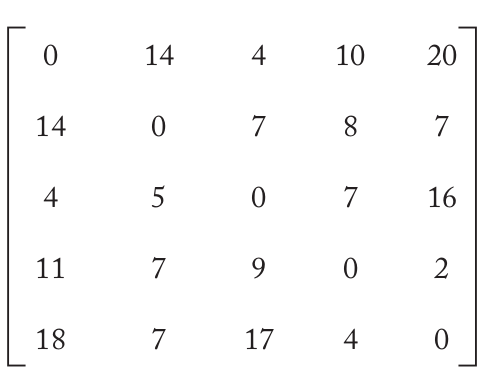
\includegraphics[width=0.2\textwidth]{figs/chap06/263-tsp-matrix}
\end{figure}
\item[-]
 کران پایین مسیر در این رأس برابراست با :
\begin{align*}
\m{14 + \sum_{i\in \{2,3,4,5 \}} min_k(V_i,V_k) = 14 + 7 + 4 + 2 + 4 = 31}
\end{align*}
\end{itemize}
\end{frame} 


\begin{frame}{مسئلهٔ فروشندهٔ دوره‌گرد}
\begin{itemize}\itemr
\item[-]
بدین ترتیب می‌توانیم مقدار کران را در هر‌یک از رئوس درخت فضای حالت به صورت زیر محاسبه کنیم.
\begin{figure}
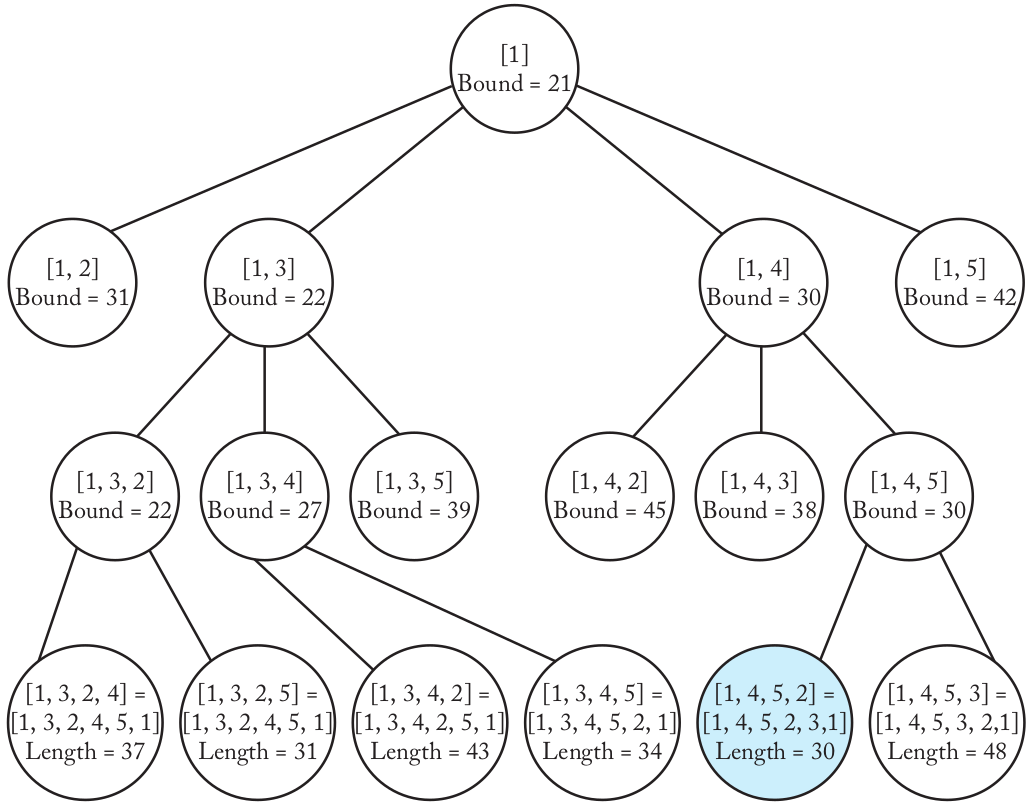
\includegraphics[width=0.5\textwidth]{figs/chap06/267-tree}
\end{figure}
\end{itemize}
\end{frame} 


\begin{frame}{مسئلهٔ فروشندهٔ دوره‌گرد}
\begin{itemize}\itemr
\item[-]
مقدار کران را برای همهٔ رئوس محاسبه می‌کنیم و رأسی را برای بسط دادن انتخاب می‌کنیم که مقدار کران آن کمینه باشد.
\item[-]
در اینجا از بین رئوس
\m{[1,2], [1,3], [1,4], [1,5]}
رأس 
\m{[1,3]}
کوچکترین کران را دارد که برابر با ۲۲ است.
\item[-]
وقتی رأس 
\m{[1,3]}
بسط داده شد، در نهایت کوتاهترین طول مسیری که در ریشه به دست می‌آید برابر با ۳۱ است.
\item[-]
اما در رأس 
\m{[1,4]}
همچنان یک کران کوچکتر برابر با ۳۰ وجود دارد،‌ بنابراین آن رأس را بسط می‌دهیم و در نهایت مسیری با طول ۳۰ پیدا می‌کنیم.
\end{itemize}
\end{frame} 


\begin{frame}{مسئلهٔ فروشندهٔ دوره‌گرد}
\begin{itemize}\itemr
\item[-]
هر رأس در درخت فضای حالت را می‌توانیم با ساختمان زیر نشان دهیم.
\begin{algorithm}[H]\alglr
\caption{Node Structure} 
\begin{algorithmic}[1]
\Statex \textbf{struct} node
\State~~ int level \LeftComment{the node’s level in the tree}
\State~~ ordered-set path
\State~~ int bound
\end{algorithmic}
\label{alg:node-structure}
\end{algorithm}
\end{itemize}
\end{frame} 


\begin{frame}{مسئلهٔ فروشندهٔ دوره‌گرد}
\begin{itemize}\itemr
\item[-]
در الگوریتم زیر برای یک گراف با n رأس، که وزن یال‌های آن با ماتریس W داده شده است، می‌خواهیم کوتاهترین دور همیلتونی را پیدا کنیم.
\begin{algorithm}[H]\alglr
  \caption{Travelling Salesman Problem} 
  \begin{algorithmic}[1]
   \Func{Travelling-Salesman-Problem}{int n, int-matrix W}
   \State ordered-set opttour \LeftComment{Optimal tour}
   \State int minlength = $\infty$ \LeftComment{The length of the optimal tour}
   \State priority-queue PQ
   \State node v
   \State initialize(PQ)		\LeftComment{Initialize PQ to be empty.}
   \State v.level = 0
   \State v.path = [1]	\LeftComment{Make first vertex the}
   \State v.bound = bound(v)		\LeftComment{starting one.}
   \State insert(PQ,v)                           
  \end{algorithmic}
  \label{alg:tsp1}
\end{algorithm}
\end{itemize}
\end{frame} 


\begin{frame}{مسئلهٔ فروشندهٔ دوره‌گرد}
\begin{center}
\resizebox{.74\textwidth}{!}{
\begin{minipage}{\textwidth}
\begin{algorithm}[H]\alglr
  \caption{Travelling Salesman Problem} 
  \begin{algorithmic}[1]
  \setcounter{ALG@line}{9}
  % \Func{Travel2}{int n, const number W[] [], ordered-set\& opttour, number\& minlength}
   \While{!empty(PQ)}
   	  \State remove(PQ, v)\LeftComment{Remove node with best bound.}
   	  \If{(v.bound < minlength)}
   			   \For{(all i not in v.path)}
   			           %\State create new node u
   			           \State create the new tree node u
   			           \State u.level = v.level + 1\LeftComment{Set u to a child of v.}
   					   \State u.path = [v.path , i] \LeftComment{put i at the end of v.path}
						\Statex \LeftComment{Check if next vertex completes a tour.}   					   
   					   \If{(u.level == n-2)}
							\Statex \LeftComment{put the last vertex not in u.path and also vertex 1 at the end of u.path}   					       
   					        \State u.path = [u.path, last-vertex, 1]
                           \Statex \LeftComment{Function length computes the length of the tour.}   							
   							\If{(length(u) < minlength)}
   									\State minlength = length(u)
   									\State opttour = u.path
   							\EndIf
   					   \Else
   							\State u.bound = bound(u)
   					        \If{(u.bound < minlength)}
   							   \State insert(PQ, u)
   					         \EndIf
   					   \EndIf
   		   \EndFor
   	   \EndIf
   \EndWhile     
   \State \Return (opttour, minlength)                         
  \end{algorithmic}
  \label{alg:tsp2}
\end{algorithm}
\end{minipage}
}
\end{center}
\end{frame}



\begin{frame}{مسئلهٔ فروشندهٔ دوره‌گرد}
\begin{itemize}\itemr
\item[-]
کران یک رأس درخت فضای حالت را به صورت زیر محاسبه می‌کنیم.
\begin{center}
\resizebox{.8\textwidth}{!}{
\begin{minipage}{\textwidth}
\begin{algorithm}[H]\alglr
\caption{Computing Bound for Travelling Salesman Problem} 
  \begin{algorithmic}[1]
   \Func{bound}{node v}
   \State bound = 0  
   \For{edge (i,j) in v.path}
       \State bound += length(i,j)
   \EndFor  
   %\State min = $\infty$
   \State i = last vertex in v.path
   \State min = $\min_k$ \{ W[i][k], vertex k $\not\in$ v.path \}
   %\For{vertex k not in v.path}
   %        \If{W[i][k] < min}
   %            \State min = W[i][k]
   %        \EndIf
   %    \EndFor  
   \State bound += min      
   \For{vertex i $\not\in$ v.path}
   \State min = $\min_k$ \{ W[i][k], vertex k $\not\in$ v.path \textbf{or} k = 1 \}
       %\State min = W[i][1]
       %\For{vertex k not in v.path}
       %    \If{W[i][k] < min}
       %        \State min = W[i][k]
       %    \EndIf
       %\EndFor
       \State bound += min
  \EndFor
  \State \Return bound
  \end{algorithmic}
  \label{alg:tsp-bound}
\end{algorithm}
\end{minipage}
}
\end{center}
\end{itemize}
\end{frame} 

\iffalse
\begin{frame}{مسئلهٔ فروشندهٔ دوره‌گرد}
\begin{itemize}\itemr
\item[-]
ممکن است در یک الگوریتم شاخه و کران بتوانیم چندین تابع کران پیدا کنیم که در این موارد معمولاً یکی از توابع، کران بهتری پیدا می‌کند.
\end{itemize}
\end{frame}
\fi

%%%%%%%%%%%%%%%%%%%%%%%%%
\section{الگوریتم‌های گراف}
%%%%%%%%%%%%%%%%%%%%%%%%%

\begin{frame}{‌الگوریتم‌های گراف}
\begin{itemize}\itemr
\item[-]
گراف یک ساختار گسسته است که با استفاده از آن می‌توان تعدادی مفهوم که با یکدیگر در ارتباط هستند را مدلسازی کرد.
\item[-]
برای مدلسازی مفاهیم از رئوس گراف و برای مدلسازی ارتباط بین مفاهیم از یال‌های گراف استفاده می‌کنیم.
\item[-]
گراف‌ها در علوم کامپیوتر و دیگر شاخه‌های علوم بسیار پر استفاده‌اند. برای مثال برای مدلسازی یک شبکهٔ کامپیوتری که از تعدادی کامپیوتر و تعدادی مسیر ارتباطی تشکیل شده است، می‌توانیم از یک گراف استفاده کنیم و از الگوریتم‌های گراف برای یافتن مسیر بهینه برای انتقال یک بسته در شبکه بهره بگیریم. همچنین در شبکه‌های اجتماعی می‌توان افراد و سازمان‌ها را به عنوان رئوس یک گراف در نظر گرفت و ارتباط بین افراد و سازمان‌ها را با استفاده از یال‌های گراف مدلسازی کرد. از الگوریتم‌های گراف جهت تحلیل این شبکه اجتماعی برای یافتن اطلاعات در گراف می‌توان استفاده کرد.
\end{itemize}
\end{frame}


\begin{frame}{‌الگوریتم‌های گراف}
\begin{itemize}\itemr
\item[-]
در زبان‌شناسی می‌توان از گراف‌ها جهت نمایش ارتباط بین کلمات در یک زبان استفاده کرد و از گراف به دست آمده در پردازش زبان طبیعی، و ترجمه‌های ماشینی استفاده کرد.
\item[-]
در علوم فیزیک و شیمی می‌توان از گراف‌ها جهت مدلسازی مولکول‌ها استفاده کرد و ساختار مولکول‌ها و روابط آنها و نیروهای بین اتم‌ها و مولکول‌ها را شبیه سازی کرد.
\item[-]
در علوم اجتماعی می‌توان از گراف‌ها جهت مدلسازی ارتباط انسان‌ها و نحوه منتشر شدن اطلاعات و افکار بین انسان‌ها و جوامع استفاده کرد.
\item[-]
در علوم زیست‌شناسی می‌توان از گراف‌ها جهت بررسی روابط بین گونه‌های جانوری و گیاهی و همچنین بررسی ساختار ژن‌ها استفاده کرد.
\end{itemize}
\end{frame}


\begin{frame}{‌الگوریتم‌های گراف}
\begin{itemize}\itemr
\item[-]
در این قسمت با روش‌های نمایش گراف و جستجوی گراف‌ها آشنا می‌شویم. با استفاده از روش‌های جستجوی گراف‌ها می‌توانیم ساختار یک گراف و ویژگی‌های آن را بشناسیم.
\end{itemize}
\end{frame}


\begin{frame}{‌الگوریتم‌های گراف}
\begin{itemize}\itemr
\item[-]
یک گراف را می‌توان با استفاده از دو مجموعهٔ رأس‌ها
\fn{1}{vertex set}
\m{(V)}
و یال‌ها
\fn{2}{edge set}
\m{(E)}
نمایش داد. بدین ترتیب دوتایی
\m{G = (V,E)}
گرافی را نمایش می‌دهد که در آن
\m{V}
مجموعه‌ای است از رئوس و
\m{E}
مجموعه‌ای است از یال‌ها. یک یال دو رأس را به یکدیگر متصل می‌کند.
\end{itemize}
\end{frame}


\begin{frame}{‌الگوریتم‌های گراف}
\begin{itemize}\itemr
\item[-]
علاوه بر روش استاندارد نمایش یک گراف توسط مجموعه‌ها، می‌توانیم یک گراف را توسط مجموعه‌ای از لیست‌های مجاورت
\fn{1}{adjacency lists}
یا یک ماتریس مجاورت
\fn{2}{adjacency matrix}
نشان دهیم.
\item[-]
توسط لیست مجاورت می‌توان گراف‌های خلوت
\fn{3}{sparse graph}
را که در آنها
\m{|E|}
بسیار کوچک‌تر از
\m{{|V|}^2}
است نمایش داد.
وقتی گراف متراکم
\fn{4}{dense}
است، می‌توان از نمایش ماتریس مجاورت استفاده کرد.
\end{itemize}
\end{frame}


\begin{frame}{‌الگوریتم‌های گراف}
\begin{itemize}\itemr
\item[-]
در نمایش لیست مجاورت
\fn{1}{adjacency-list representation}
برای گراف
\m{G = (V,E)}
از آرایهٔ
\m{Adj}
شامل
\m{|V|}
عنصر استفاده می‌کنیم. به ازای هر
\m{u \in V}
،
لیست مجاورت
\m{Adj[u]}
شامل رئوس
\m{v}
 است به طوری‌که
\m{(u,v) \in E}
. پس
\m{Adj[u]}
شامل همهٔ رئوسی است که در گراف
\m{G}
مجاور
\m{u}
هستند. در پیاده‌سازی این روش،
عناصر این آرایه می‌توانند اشاره‌گر به رئوس مجاور باشند.
\end{itemize}
\end{frame}


\begin{frame}{‌الگوریتم‌های گراف}
\begin{itemize}\itemr
\item[-]
در شکل زیر دو گراف توسط لیست مجاورت نشان داده شده‌اند.
\begin{figure}
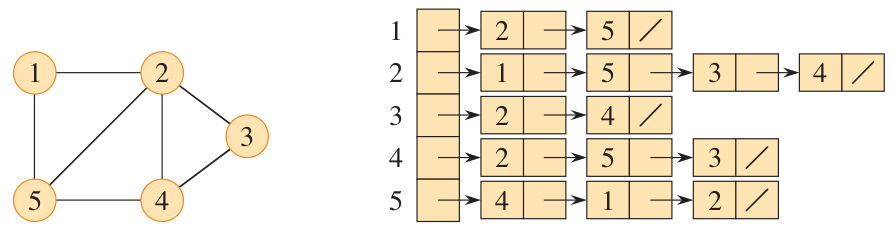
\includegraphics[width=0.6\textwidth]{figs/chap07/550-graph1-adj}
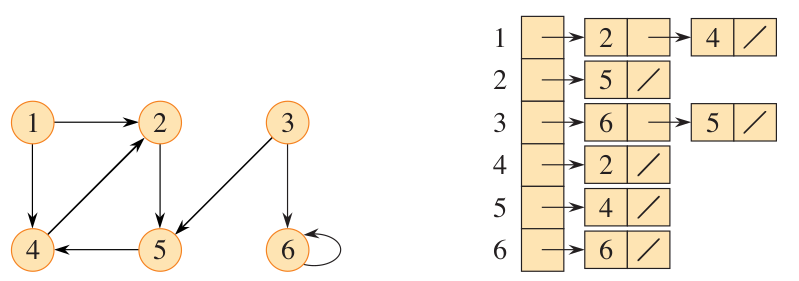
\includegraphics[width=0.6\textwidth]{figs/chap07/550-graph2-adj}
\end{figure}
\end{itemize}
\end{frame}


\begin{frame}{‌الگوریتم‌های گراف}
\begin{itemize}\itemr
\item[-]
اگر
\m{G}
یک گراف جهت‌دار باشد، مجموع اندازه همهٔ لیست‌های مجاورت برابراست با
\m{|E|}
، زیرا هریک از یال‌های
\m{(u,v)}
توسط درایهٔ
\m{Adj[u]}
نشان داده می‌شود.
\item[-]
اگر
\m{G}
یک گراف بدون جهت باشد، آنگاه مجموع اندازهٔ همهٔ لیست‌های مجاورت برابراست با
\m{2|E|}
، زیرا هر یک از یال‌های
\m{(u,v)}
هم در
\m{Adj[u]}
و هم در
\m{Adj[v]}
نمایش داده می‌شود.
\item[-]
فضای حافظه‌ای که لیست مجاورت برای نگهداری گراف نیاز دارد برابراست با
\ath{V+E} .
\iffalse
یافتن یک یال در گراف نیز به زمان
\ath{V+E}
نیاز دارد، زیرا برای یافتن یک یال همهٔ
\m{|V|}
درایهٔ لیست مجاورت باید بررسی شوند.
\fi
\end{itemize}
\end{frame}


\begin{frame}{‌الگوریتم‌های گراف}
\begin{itemize}\itemr
\item[-]
توسط لیست مجاورت می‌توانیم گراف‌های وزن‌دار
\fn{1}{weighted graphs}
را نیز نمایش دهیم.
در یک گراف وزن‌دار، هریک از یال‌ها دارای یک وزن است که توسط تابع وزن
\fn{2}{weight function}
\m{w : E \rightarrow \RR}
تولید می‌شود.
\item[-]
برای مثال فرض کنید
\m{G = (V,E)}
یک گراف وزن‌دار با تابع وزن
\m{w}
باشد. آنگاه می‌توانیم وزن
\m{w(u,v)}
از یال
\m{(u,v) \in E}
را در کنار رأس
\m{v}
در لیست مجاورت
\m{u}
ذخیره کنیم و نمایش دهیم.
\item[-]
یکی از معایب لیست مجاورت این است که برای پیدا کردن یال
\m{(u,v)}
سریع‌ترین روش ممکن جستجوی
\m{v}
در لیست مجاورت
\m{Adj[u]}
است.
\item[-]
ماتریس مجاورت برای پیدا کردن یک یال می‌تواند از لیست مجاورت سریع‌تر عمل کند.
\end{itemize}
\end{frame}


\begin{frame}{‌الگوریتم‌های گراف}
\begin{itemize}\itemr
\item[-]
در نمایش ماتریس مجاورت
\fn{1}{adjacency matrix representation}
برای گراف
\m{G = (V,E)}
فرض می‌کنیم هر رأس یک شماره از 
\m{1}
 تا
\m{|V|}
داشته باشد. سپس گراف
\m{G}
را با استفاده از ماتریس
\m{A = (a_{ij})}
با اندازهٔ
\m{|V| \times |V|}
نشان می‌دهیم به طوری‌که
\begin{align*}
\m{a_{ij}}  = \left\{ \begin{array}{lr}
				\m{1} & \m{(i,j) \in E}~\text{اگر}\\
					\m{0} & \text{در غیر اینصورت}
					\end{array}\right.
\end{align*}
\end{itemize}
\end{frame}


\begin{frame}{‌الگوریتم‌های گراف}
\begin{itemize}\itemr
\item[-]
در شکل زیر دو ماتریس مجاورت نشان داده شده‌اند.
\begin{figure}
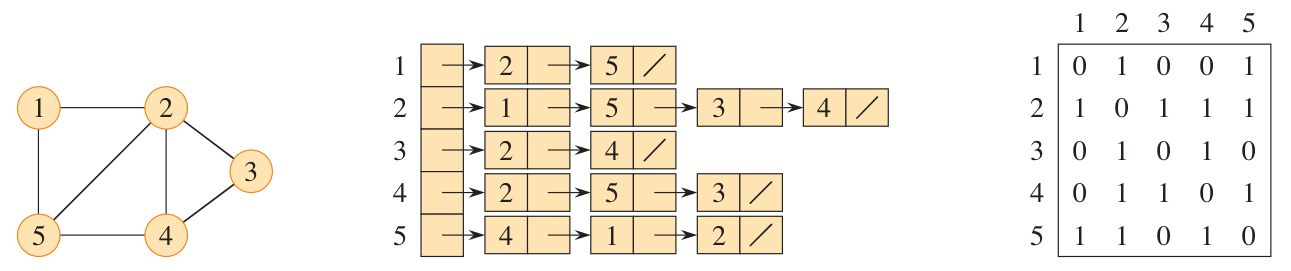
\includegraphics[width=0.9\textwidth]{figs/chap07/550-graph1}
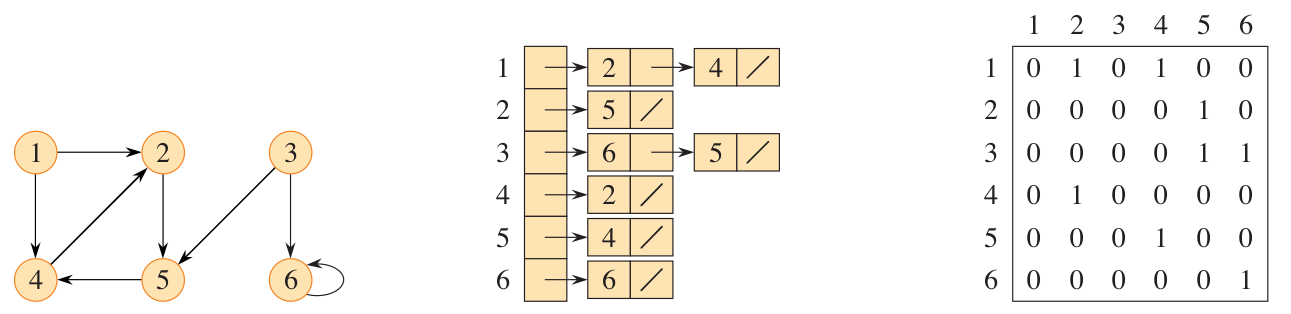
\includegraphics[width=0.9\textwidth]{figs/chap07/550-graph2}
\end{figure}
\end{itemize}
\end{frame}


\begin{frame}{‌الگوریتم‌های گراف}
\begin{itemize}\itemr
\item[-]
ماتریس مجاورت به حافظه
\ath{V^2}
برای نگهداری گراف نیاز دارد. برای یافتن یال
\m{(u,v)}
در گراف می‌توانیم درایهٔ
\m{A[u,v]}
را بررسی کنیم و بنابراین یافتن یک یال در گراف در زمان
\ath{1}
انجام می‌شود.
\item[-]
برای یک گراف بدون جهت، گراف نسبت به قطر اصلی‌اش متقارن است، زیرا
\m{A[u,v]}
برابراست با
\m{A[v,u]}
بنابراین ماتریس مجاورت برابر با ترانهادهٔ
\fn{1}{transpose}
 آن است و داریم
\m{A = A^T} .
\item[-]
اما در یک گراف جهت‌دار می‌توانیم یالی از
\m{u}
به
\m{v}
داشته باشیم بدون اینکه یال از
\m{v}
به
\m{u}
وجود داشته باشد.
\end{itemize}
\end{frame}


\begin{frame}{‌الگوریتم‌های گراف}
\begin{itemize}\itemr
\item[-]
با استفاده از ماتریس مجاورت می‌توانیم یک گراف وزن‌دار را نیز نمایش دهیم.
\item[-]
برای مثال، اگر
\m{G = (V,E)}
یک گراف وزن‌دار با تابع وزن
\m{w}
باشد، می‌توان وزن
\m{w(u,v)}
برای یال
\m{(u,v) \in E}
را به عنوان درایهٔ ماتریس مجاورت در سطر
\m{u}
و ستون
\m{v}
ذخیره کرد.
\item[-]
استفاده از ماتریس مجاورت در عمل راحت‌تر است اما به ازای گراف‌های بزرگ خلوت ممکن است فضای حافظه مورد نیاز آنها بسیار زیاد شود.
برای ذخیره‌سازی گراف‌های خلوت جهت‌دار، لیست مجاورت نسبت به ماتریس مجاورت فضای بسیار کمتری اشغال می‌کند.
\end{itemize}
\end{frame}

\begin{frame}{‌جستجوی سطح‌اول}
\begin{itemize}\itemr
\item[-]
جستجوی سطح‌اول
\fn{1}{breadth-first search}
یکی از ساده‌ترین الگوریتم‌های جستجوی گراف است که در بسیاری از الگوریتم‌های گراف استفاده می‌شود. برای مثال الگوریتم دایکسترا برای یافتن کوتاهترین مسیر بین دو رأس از جستجوی سطح‌اول استفاده می‌کند.
\item[-]
به ازای گراف دلخواه
\m{G=(V,E)}
و یک رأس مبدأ
\fn{2}{source vertic}
به نام
\m{s}
، الگوریتم جستجوی سطح‌اول همهٔ یال‌های گراف
\m{G}
را با شروع از رأس
\m{s}
بررسی می‌کند.
\item[-]
با شروع از رأس
\m{s}
، الگوریتم سطح‌اول ابتدا رئوسی را بررسی می‌کند که به
\m{s}
نزدیک‌ترند،
بدین معنی که برای رسیدن به آن رئوس از
\m{s}
باید از تعداد یال‌های کمتری عبور کرد.
\end{itemize}
\end{frame}


\begin{frame}{‌جستجوی سطح‌اول}
\begin{itemize}\itemr
\item[-]
یال‌هایی که در جستجوی سطح‌اول به ترتیب بررسی می‌شوند، یک درخت سطح‌اول می‌سازد که ریشهٔ آن
\m{s}
است و به ازای هر یک از رئوس
\m{v}
، یک مسیر ساده از
\m{s}
به
\m{v}
کوتاهترین مسیر از
\m{s}
به
\m{v}
در گراف را نشان می‌دهد.
در اینجا کوتاهترین مسیر درواقع مسیری است که دارای کمترین تعداد یال باشد.
\item[-]
جستجوی سطح‌اول، بدین دلیل سطح‌اول نامیده می‌شود که به ازای هر رأس
\m{v}
ابتدا رئوس مجاور آن بررسی  می‌شوند، قبل از اینکه رئوس مجاور مجاور آن بررسی شوند.
بنابراین اگر نزدیکترین رئوس به یک رأس را در سطح در نظر بگیریم و دورترین رئوس را در عمق، جستجوی سطح‌اول، قبل از بررسی رئوس در عمق، همهٔ رئوس در سطح را بررسی می‌کند.
بنابراین برخلاف جستجوی عمق اول که به ازای هر رأس
\m{v}
یک رأس مجاور مجاور
\m{v}
 ممکن است قبل از یک رأس مجاور
\m{v}
  پیمایش شود، در جستجوی سطح‌اول همهٔ رئوس مجاور
\m{v}
قبل از پیمایش رئوس مجاور مجاور 
\m{v}
پیمایش می‌شوند.
\end{itemize}
\end{frame}


\begin{frame}{‌جستجوی سطح‌اول}
\begin{itemize}\itemr
\item[-]
 در جستجوی سطح‌اول با شروع از رأس
\m{s}
ابتدا رئوس مجاور
\fn{1}{adjacent}
 یا همسایه‌هایی
\fn{2}{neighbour}
  بررسی می‌شوند که فاصلهٔ آنها از
\m{s}
برابر ۱ است، سپس همسایه‌ها با فاصلهٔ ۲ بررسی می‌شوند، پس از آن همسایه‌ها با فاصلهٔ ۳ و به همین ترتیب الی آخر، تا وقتی که همه رئوس بررسی شده باشند.
\item[-]
در جستجوی سطح‌اول از یک صف استفاده می‌شود که در آن ابتدا همسایه‌ها با فاصله ۱، سپس همسایه‌ها با فاصلهٔ ۲ و به همین ترتیب الی آخر در صف قرار می‌گیرند. بنابراین با خارج کردن همسایه‌ها از صف به ترتیب فاصله، گراف به صورت سطح‌اول بررسی می‌شود.
\end{itemize}
\end{frame}


\begin{frame}{‌جستجوی سطح‌اول}
\begin{itemize}\itemr
\item[-]
در الگوریتم جستجوی سطح‌اول می‌توانیم برای هر رأس ۳ رنگ در نظر بگیریم : سفید، خاکستری و سیاه. همهٔ رئوس در ابتدا به رنگ سفید هستند و رئوسی که هیچ مسیری از
\m{s}
به آنها وجود ندارد تا انتها به رنگ سفید باقی می‌‌مانند. وقتی یک رأس برای اولین بار با شروع از
\m{s}
پیمایش می‌شود، آن رأس به رنگ خاکستری تبدیل می‌شود. رنگ خاکستری بدین معنی است که آن رأس در مرز جستجو قرار گرفته است. مرز جستجو در واقع مرز میان رئوس پیمایش نشده و رئوس پیمایش شده است. صفی که در جستجوی سطح‌اول استفاده می‌شود، شامل همهٔ رئوس خاکستری است.
\item[-]
رئوس خاکستری به ترتیب از صف خارج می‌شوند و به رنگ سیاه تبدیل می‌شوند و رئوس سفید همسایهٔ آنها که تاکنون پیمایش نشده‌اند به رنگ خاکستری تبدیل می‌شوند و وارد صف می‌شوند.
\end{itemize}
\end{frame}


\begin{frame}{‌جستجوی سطح‌اول}
\begin{itemize}\itemr
\item[-]
یک الگوریتم جستجوی سطح‌اول، یک درخت سطح‌اول می‌سازد که ریشهٔ آن رأس
\m{s}
است. هرگاه در فرایند جستجو، یک رأس سفید
\m{v}
که در لیست همسایه‌های رأس خاکستری
\m{u}
 قرار دارد پیدا می‌شود، رأس
\m{v}
و یال
\m{(u,v)}
به درخت اضافه می‌شوند. می‌گوییم رأس
\m{u}
، سَلَف
\fn{1}{predecessor}
یا پدر رأس
\m{v}
و رأس
\m{v}
خَلَف
\fn{2}{successor}
یا فرزند رأس
\m{u}
در درخت سطح‌اول است. از آنجایی که هر رأس قابل دسترس از طریق
\m{s}
تنها یک بار بررسی می‌شود، هر رأس تنها یک پدر دارد.
\item[-]
تنها رأس ریشه، یعنی رأس
\m{s}
  دارای پدر نیست.
\item[-]
اگر رأس
\m{u}
بر روی یک مسیر ساده درخت از ریشه
\m{s}
به رأس
\m{v}
قرار بگیرد، آنگاه رأس
\m{u}
جد
\fn{3}{ancestor}
رأس
\m{v}
است و رأس
\m{v}
نوادهٔ
\fn{4}{descendant}
رأس
\m{u}
است.
\end{itemize}
\end{frame}


\begin{frame}{‌جستجوی سطح‌اول}
\begin{itemize}\itemr
\item[-]
در الگوریتم جستجوی سطح‌اول که بررسی خواهیم کرد،
\code{v.color}
رنگ رأس
\m{v}
است که می‌تواند سفید، خاکستری یا سیاه باشد،
\code{v.d}
فاصلهٔ رأس
\m{v}
از رأس
\m{s}
است و
\code{v.pred}
پدر رأس
\m{v}
است.
\item[-]
 رأس
\code{v.pred}
پدر
\fn{1}{predecessor}
 رأس
\code{v}
است، و رأس
\code{v}
فرزند
\fn{2}{successor}
رأس
\code{v.pred}
.
\end{itemize}
\end{frame}


\begin{frame}{‌جستجوی سطح‌اول}
\begin{itemize}\itemr
\item[-]
الگوریتم زیر جستجوی سطح‌اول را نشان می‌دهد.
\begin{algorithm}[H]\alglr
  \caption{Breadth-First Search} 
  \begin{algorithmic}[1]
   \Func{BFS}{G,s}
   \For{each vertex u $\in$ G.V - \{s\} }
   			\State u.color = White
   			\State u.d = $\infty$
   			\State u.pred = Nil
   	\EndFor
   	\State s.color = Gray
   	\State s.d = 0
   	\State s.pred = Nil
   	\State Q = $\emptyset$
   	\State Enqueue(Q,s)         
  \end{algorithmic}
  \label{alg:merge}
\end{algorithm}
\end{itemize}
\end{frame}


\begin{frame}{‌جستجوی سطح‌اول}
\begin{algorithm}[H]\alglr
  \caption{Breadth-First Search} 
  \begin{algorithmic}[1]
  \setcounter{ALG@line}{9}
   %\Func{Bfs}{G,s}			%\LeftComment{}
        \While{!empty(Q)}
        		\State u = Dequeue(Q)
        		\For{each vertex v in G.Adj[u]}		\LeftComment{search the neighbors of u}
        			\If{v.color == White}		\LeftComment{is v being discovered now?}
        				\State v.color = Gray
        				\State v.d = u.d + 1
        				\State v.pred = u
        				\State Enqueue(Q,v)		\LeftComment{v is now on the frontier}
        			\EndIf
        		\EndFor
        		\State u.color = Black		\LeftComment{u is now behind the frontier}
        \EndWhile		                   
  \end{algorithmic}
  \label{alg:merge}
\end{algorithm}
\end{frame}


\begin{frame}{‌جستجوی سطح‌اول}
\begin{itemize}\itemr
\item[-]
در شکل زیر یک گراف به صورت سطح‌اول پیمایش شده است.
\begin{figure}
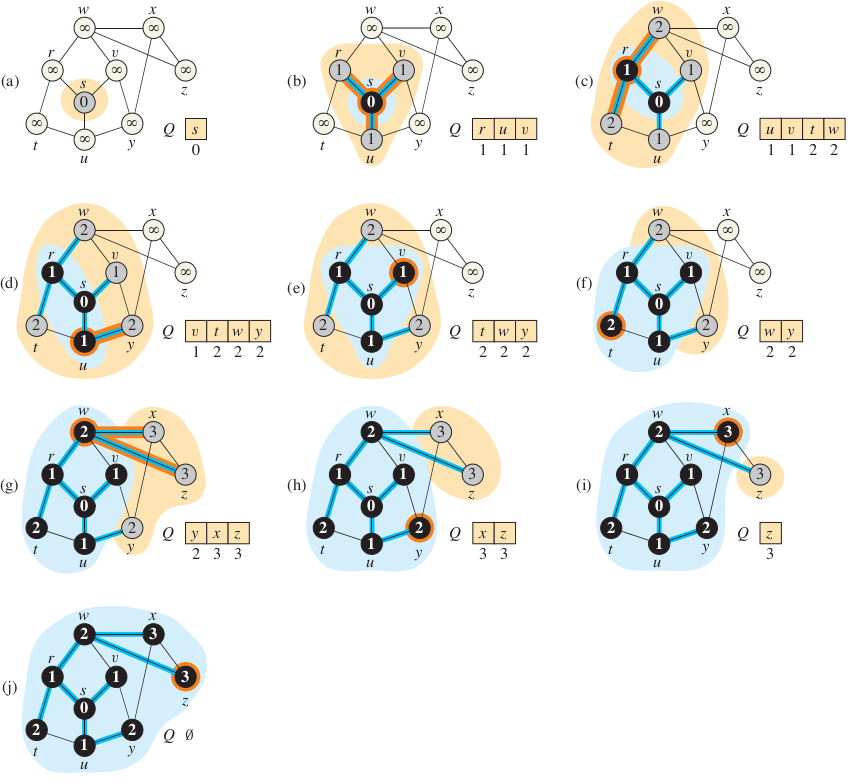
\includegraphics[width=0.5\textwidth]{figs/chap07/557-bfs}
\end{figure}
\end{itemize}
\end{frame}


\begin{frame}{‌جستجوی سطح‌اول}
\begin{itemize}\itemr
\item[-]
تحلیل الگوریتم جستجوی سطح‌اول : برای تحلیل الگوریتم جستجوی سطح‌اول می‌توانیم از تحلیل تجمعی استفاده کنیم. در این الگوریتم هیچ‌گاه یک رأس از رنگ خاکستری یا سیاه به رنگ سفید در نمی‌آید. هر رأس حداکثر یک بار وارد صف می‌شود و بنابراین هر رأس حداکثر یک بار از صف خارج می‌شود. عملیات اضافه کردن و برداشتن از صف در زمان
\m{O(1)}
انجام می‌شود.
خارج کردن رئوس از صف در زمان
\m{O(V)}
انجام می‌گیرد.
همچنین بررسی لیست مجاورت هر رأس حداکثر یک‌بار انجام می‌شود و مجموع طول همهٔ لیست‌های مجاورت برابر است با
\ath{E}
، بنابراین زمان لازم برای اجرای الگوریتم برابراست با
\m{O(V+E)}~.
نتیجه می‌گیریم جستجوی سطح‌اول در زمان خطی نسبت به اندازه لیست مجاورت اجرا می‌شود.
\item[-]
می‌توان ثابت کرد الگوریتم جستجوی سطح‌اول کوتاهترین مسیر از
\m{s}
به هریک از رئوس را محاسبه می‌کند.
\end{itemize}
\end{frame}

\iffalse
\begin{frame}{‌جستجوی سطح‌اول}
\begin{itemize}\itemr
\item[-]
حال می‌خواهیم اثبات کنیم الگوریتم جستجوی سطح‌اول کوتاهترین مسیر از رأس مبدأ
\m{s}
به هریک از رئوس گراف را پیدا می‌کند. فاصله کوتاهترین مسیر
\fn{1}{shortest path distance}
\m{\delta(s,v)}
از رأس
\m{s}
به
\m{v}
کمترین تعداد یال‌هایی است که در یک مسیر از
\m{s}
به
\m{v}
می‌توان پیمود. اگر هیچ مسیری از
\m{s}
به
\m{v}
وجود نداشته باشد، آنگاه
\m{\delta(s,v) = \infty}
مسیری که طول آن
\m{\delta(s,v)}
باشد کوتاهترین مسیر
\fn{2}{shortest path}
از
\m{s}
به
\m{v}
است.
\end{itemize}
\end{frame}
\fi

\begin{frame}{‌جستجوی عمق‌اول}
\begin{itemize}\itemr
\item[-]
جستجوی عمق‌اول به جای اینکه جستجو را در سطح شروع کند و همهٔ رئوس مجاور را در ابتدا پیمایش کند، به ازای هر رأس پیمایش شده، مجاور رأس را پیمایش می‌کند و به عبارت دیگر جستجو در عمق انجام می‌دهد.
\item[-]
برای روشن‌تر شدن جستجوی سطحی و عمقی مثال زیر را در نظر بگیرید. می‌خواهیم مطلبی را درون چندین کتاب جستجو کنیم. در یک جستجوی سطحی ابتدا به سراغ صفحه اول همهٔ کتاب‌ها می‌رویم تا این که در نهایت همهٔ کتاب‌ها را بررسی کنیم. در یک جستجوی عمقی ابتدا کتاب اول را تا انتها مطالعه می‌کنیم و در صورتی که مطلب مورد نظر را پیدا نکردیم به سراغ کتاب دوم می‌رویم تا این که در نهایت همهٔ کتاب‌ها را جستجو کنیم. در این مثال هیچ یک از جستجوها مزیتی بر دیگری ندارد چرا که مطلب مورد نظر ممکن است در صفحهٔ آخر کتاب اول باشد که در این صورت جستجوی عمقی زودتر به جواب می‌رسد و یا ممکن است مطلب مورد نظر در صفحه اول کتاب آخر باشد که در این صورت جستجوی سطح اول زودتر به جواب می‌رسد.
\end{itemize}
\end{frame}


\begin{frame}{‌جستجوی عمق‌اول}
\begin{itemize}\itemr
\item[-]
جستجوی عمق‌اول یال‌های بررسی نشدهٔ رئوس تازه پیدا شده را زودتر از یال‌های بررسی نشدهٔ رئوس قبلاً پیدا شده بررسی می‌کند. وقتی فرایند جستجو به نقطه‌ای رسید که یال‌های یک رأس همگی بررسی شده بودند، الگوریتم پسگرد می‌کند تا به رئوسی برسد که یال‌های آنها هنوز بررسی نشده‌اند.
\item[-]
در صورتی که یک رأس با شروع از رأس آغازین قابل دسترس نباشد، گراف همبند نیست و برای جستجوی کامل گراف، الگوریتم یکی از رئوس را به عنوان مبدأ جدید انتخاب کرده و جستجو را از رأس جدید آغاز می‌‌کند.
\end{itemize}
\end{frame}


\begin{frame}{‌جستجوی عمق‌اول}
\begin{itemize}\itemr
\item[-]
همانند جستجوی سطح اول، در جستجوی عمق‌اول توسط رنگ رأس‌ها وضعیت آنها مشخص می‌شود. هر رأس در ابتدا سفید است، هنگامی که برای اولین بار پیدا می‌شود به رنگ خاکستری تبدیل می‌شود و در پایان هنگامی که بررسی شد (بدین معنی که همهٔ رئوس در لیست مجاورت آن پیدا شدند) به رنگ سیاه در می‌آید.
\end{itemize}
\end{frame}


\begin{frame}{‌جستجوی عمق‌اول}
\begin{itemize}\itemr
\item[-]
در جستجوی عمق‌اول هر رأس دارای دو برچسب زمان
\fn{1}{time stamp}
است. برچسب زمان اول
\m{v.s}
زمانی نشان می‌دهد که رأس برای بار اول پیدا شده است و به رنگ خاکستری درآمده است و برچسب دوم
\m{v.f}
مشخص می‌کند که رأس
\m{v}
به طور کامل بررسی شده است بدین معنی که همهٔ رئوس لیست مجاورت آن پیدا شده‌اند و رأس
\m{v}
به رنگ مشکی درآمده است.
\end{itemize}
\end{frame}


\begin{frame}{‌جستجوی عمق‌اول}
\begin{itemize}\itemr
\item[-]
الگوریتم زیر جستجوی عمق‌اول را نشان می‌دهد.
\begin{algorithm}[H]\alglr
  \caption{Depth-First Search} 
  \begin{algorithmic}[1]
   \Func{DFS}{G}
   \For{each vertex u $\in$ G.V}
   			\State u.color = White
   			\State u.pred = Nil
   	\EndFor
   	\State time = 0
   	\For{each vertex u $\in$ G.V}
   			\If{u.color == White}
   					\State DFS-Visit(G,u)
   			\EndIf
   	\EndFor                           
  \end{algorithmic}
  \label{alg:merge}
\end{algorithm}
\end{itemize}
\end{frame}


\begin{frame}{‌جستجوی عمق‌اول}
\begin{itemize}\itemr
\item[-]
\begin{algorithm}[H]\alglr
  \caption{DFS-Visit} 
  \begin{algorithmic}[1]
   \Func{DFS-Visit}{G,u}
   \State time = time + 1		\LeftComment{white vertex u has just been discovered}
   \State u.s = time
   \State u.color = Gray
   \For{each vertex v in G.Adj[u]}		\LeftComment{explore each edge(u,v)}
   		\If{v.color == White}
   				\State v.pred = u
   				\State DFS-Visit(G,v)
   		\EndIf
   \EndFor
   \State time = time + 1
   \State u.f = time
   \State u.color = Black   \LeftComment{blacken u; it is finished}                           
  \end{algorithmic}
  \label{alg:merge}
\end{algorithm}
\end{itemize}
\end{frame}


\begin{frame}{‌جستجوی عمق‌اول}
\begin{itemize}\itemr
\item[-]
وقتی الگوریتم جستجوی عمق‌اول به اتمام می‌رسد هر رأس دارای دو برچسب زمان است که یکی زمان پیدا شدن
\fn{1}{discovery time}
و دیگری زمان به پایان رسیدن
\fn{2}{finish time}
را نشان می‌دهد.
\end{itemize}
\end{frame}


\begin{frame}{‌جستجوی عمق‌اول}
\begin{itemize}\itemr
\item[-]
در مثال زیر، گراف توسط الگوریتم عمق‌اول بررسی شده است.
\begin{figure}
\includegraphics[width=0.6\textwidth]{figs/chap07/566-dfs}
\end{figure}
\end{itemize}
\end{frame}


\begin{frame}{‌جستجوی عمق‌اول}
\begin{itemize}\itemr
%\item[-]
%خطوط ۱ تا ۳ و خطوط ۵ تا ۷ در الگوریتم جستجوی عمق‌اول در زمان
%\ath{V}
%انجام می‌شوند.
\item[-]
در اینجا نیز برای تحلیل الگوریتم از تحلیل تجمعی استفاده می‌کنیم.
\item[-]
الگوریتم
\code{DFS-Visit}
برای هر رأس
\m{v \in V}
تنها یک بار فراخوانی می‌شود، چرا که این الگوریتم برای رئوس سفید فراخوانی می‌شود و آنها را به رنگ خاکستری تبدیل می‌کند. الگوریتم
\code{DFS-Visit}
به ازای هر رأس
\m{v}
در یک حلقه تکرار
\m{|Adj[v]|}
بار تکرار می‌شود. بنابراین برای همهٔ رئوس، این حلقه
\m{\sum_{v \in V} |Adj[v]| = \ath{E}}
بار تکرار می‌شود.
\item[-]
پس زمان اجرای الگوریتم جستجوی عمق‌اول
\ath{V+E}
است.
\end{itemize}
\end{frame}


\begin{frame}{‌جستجوی عمق‌اول}
\begin{itemize}\itemr
\item[-]
می‌توان اثبات کرد که در جستجوی عمق‌اول زمان پیدا شدن و زمان به اتمام رسیدن رئوس گراف یک ساختار پرانتز گذاری کامل دارند. اگر به ازای یافته شدن رأس
\m{u}
یک پرانتز به صورت
\m{"(u"}
باز کنیم و به ازای به اتمام رسیدن بررسی رأس
\m{u}
پرانتز را به صورت
\m{"u)"}
ببندیم، یک عبارت با پرانتزگذاری کامل به دست می‌آید بدین معنی که پرانتزها تودرتو هستند.
\end{itemize}
\end{frame}


\begin{frame}{‌جستجوی عمق‌اول}
\begin{itemize}\itemr
\item[-]
از جستجوی عمق‌اول در مرتب‌سازی توپولوژیکی
\fn{1}{topological sort}
یا مرتب‌سازی موضعی
یک گراف بدون دور
\fn{2}{acyclic graph}
استفاده می‌شود.
\item[-]
یک مرتب‌سازی توپولوژیکی در یک گراف بدون دور
\m{G=(V,E)}
رئوس گراف را به گونه‌ای مرتب می‌کند که اگر
\m{G}
شامل یال
\m{(u,v)}
باشد، آنگاه
\m{u}
قبل از
\m{v}
در آرایهٔ مرتب شده قرار می‌گیرد.
\item[-]
مرتب‌سازی توپولوژیکی تنها برای گراف‌های جهت‌دار بدون دور
\fn{3}{directed acyclic graph}
تعریف می‌شود.
\item[-]
مرتب‌سازی توپولوژیکی به گونه‌ای است که اگر رئوس مرتب شده برروی یک خط افقی قرار بگیرند، جهت همهٔ یال‌های از چپ به راست است.
\end{itemize}
\end{frame}


\begin{frame}{‌جستجوی عمق‌اول}
\begin{itemize}\itemr
\item[-]
از یک گراف جهت‌دار بدون دور می‌توان برای نمایش دادن رویداد‌ها
\fn{1}{event}
استفاده کرد.
\item[-]
برای مثال در شکل زیر برای یک گراف شامل تعدادی رویداد مرتب‌سازی توپولوژیکی انجام شده است.
\begin{figure}
\includegraphics[width=0.6\textwidth]{figs/chap07/574-topological}
\end{figure}
\end{itemize}
\end{frame}

\begin{frame}{‌درخت پوشای کمینه}
\begin{itemize}\itemr
\item[-]
در طراحی مدارهای الکتریکی، معمولاً طراحان نیاز دارند که قسمت‌هایی از مدار را که در یک سطح ولتاژ قرار دارند، به یکدیگر متصل کنند. برای متصل کردن
\m{n}
نقطه به یکدیگر، به
\m{n-1}
سیم نیاز داریم که به شکل‌های متفاوت می‌توانند هر یک  دو نقطه را به یکدیگر متصل کنند. در چنین مسئله‌ای هدف یافتن روشی برای اتصال است که در آن از کمترین مقدار سیم لازم استفاده می‌کنیم. برای مدلسازی این مسئله به صورت زیر عمل می‌کنیم.
\item[-]
گراف
\m{G = (V,E)}
را با وزن‌های
\m{w : E \to \RR}
در نظر بگیرید. وزن یال
\m{(u,v) \in E}
برابر است با
\m{w(u,v)} .
\end{itemize}
\end{frame}


\begin{frame}{‌درخت پوشای کمینه}
\begin{itemize}\itemr
\item[-]
نقطه‌ها در یک مدار الکتریکی معادل رئوس گراف و سیم‌ها معادل یال‌های گراف هستند. مقدار سیمی که برای اتصال یک نقطه به نقطه دیگر نیاز است را با وزن یال مدلسازی می‌کنیم.
\item[-]
هدف پیدا کردن زیر مجموعهٔ
\m{ T \subseteq E}
است که همهٔ رئوس گراف را به یکدیگر متصل می‌کند و وزن کل آن برابر با
\m{w(T) = \sum_{(u,v) \in T} w(u,v)}
کمینه است.
\item[-]
زیرمجموعهٔ
\m{ T }
همهٔ رأس‌های گراف را به یکدیگر متصل می‌کند و دارای هیچ دوری نیست، پس یک درخت را تشکیل می‌دهد. به چنین درختی، درخت پوشا
\fn{1}{spanning tree}
گفته می‌شود. مسئله درخت پوشای کمینه
\fn{2}{minimum spanning tree problem}
به دنبال درخت پوشایی می‌گردد که وزن آن از همهٔ درخت‌های پوشای دیگر کمتر باشد.
\end{itemize}
\end{frame}


\begin{frame}{‌درخت پوشای کمینه}
\begin{itemize}\itemr
\item[-]
ورودی مسئله درخت پوشای کمینه گراف همبند بدون جهت
\m{G = (V,E)}
است که تابع وزن یال‌های آن
\m{w : E \rightarrow \RR}
است. هدف یافتن یک درخت پوشای کمینه برای
\m{G}
است.
\item[-]
دو الگوریتم حریصانه برای یافتن درخت پوشای کمینه معرفی خواهیم کرد که روش آنها مشابه است ولی پیاده‌سازی آنها متفاوت است.
\item[-]
این استراتژی را به عنوان یک الگوریتم کلی برای یافتن درخت پوشای کمینه معرفی می‌کنیم.
\end{itemize}
\end{frame}


\begin{frame}{‌درخت پوشای کمینه}
\begin{itemize}\itemr
\item[-]
الگوریتم کلی برای یافتن درخت پوشای کمینه به صورت زیر است.
\begin{algorithm}[H]\alglr
  \caption{Generic-MST} 
  \begin{algorithmic}[1]
   \Func{Generic-MST}{G,w}
   \State A =$\emptyset$
   \While{A does not form a spanning tree}
   			\State find an edge (u,v) that is safe for A
   			\State A = A $\cup$ {(u,v)}
   	\EndWhile
   	\State \Return A               
  \end{algorithmic}
  \label{alg:merge}
\end{algorithm}
\end{itemize}
\end{frame}


\begin{frame}{‌درخت پوشای کمینه}
\begin{itemize}\itemr
\item[-]
قبل از هر تکرار در حلقه،
\m{A}
یک زیر مجموعه از یک درخت پوشای کمینه است.
\item[-]
در هر گام از الگوریتم، یال
\m{(u,v)}
به
\m{A}
اضافه می‌شود بدون اینکه ویژگی
\m{A}
تغییر کند. به عبارت دیگر
\m{A \cup {(u,v)}}
نیز زیرمجموعه‌ای از درخت پوشای کمینه است.
\item[-]
یالی که به
\m{A}
اضافه می‌شود را یک یال مطمئن
\fn{1}{safe edge}
می‌نامیم زیرا ویژگی درخت را حفظ می‌کند.
\item[-]
پس در گام اول قبل از شروع حلقه ویژگی درخت (که زیرمجموعهٔ درخت پوشای کمینه است) برقرار است. در هرگام در حلقه تکرار ویژگی درخت حفظ می‌شود، پس در پایان یک درخت پوشای کمینه خواهیم داشت.
\end{itemize}
\end{frame}


\begin{frame}{‌درخت پوشای کمینه}
\begin{itemize}\itemr
\item[-]
حال روشی برای یافتن یال مطمئن ارائه می‌‌دهیم.
\item[-]
قبل از بررسی ویژگی یال مطمئن چند تعریف ارائه می‌کنیم.
\item[-]
یک برش
\fn{1}{cut}
\m{(S,V-S)}
از یک گراف بدون جهت
\m{G = (V,E)}
یک تقسیم‌بندی از رئوس
\m{V}
است که در آن مجموعهٔ رئوس به دو قسمت تقسیم می‌شوند.
\item[-]
می‌گوییم یال
\m{(u,v) \in E}
از برش
\m{(S,V-S)}
عبور می‌کند
\fn{1}{crosses}
اگر یک رأس یال در مجموعهٔ
\m{S}
و رأس دیگر یال در مجموعهٔ
\m{V-S}
قرار بگیرد.
\item[-]
یالی را که از یک برش عبور می‌کند یال سبک
\fn{3}{light edge}
می‌نامیم اگر وزن آن در بین همهٔ یال‌هایی که از برش عبور می‌کنند کمینه باشد. در یک برش ممکن است چند یال سبک هم‌وزن وجود داشته باشند.
\end{itemize}
\end{frame}


\begin{frame}{‌درخت پوشای کمینه}
\begin{itemize}\itemr
\item[-]
شکل زیر یک برش را نشان می‌دهد.
یال سبک در این برش یال 
\m{(c, d)}
با وزن ۷ است.
\begin{figure}
\includegraphics[width=0.9\textwidth]{figs/chap07/588-cut}
\end{figure}
\end{itemize}
\end{frame}


\begin{frame}{‌درخت پوشای کمینه}
\begin{itemize}\itemr
\item[-]
قضیه : فرض کنید
\m{G = (V,E)}
یک گراف همبند بدون جهت با یال‌های وزن‌دار باشد و وزن‌ها با تابع
\m{w}
تعریف شده باشند. فرض کنید
\m{A}
یک زیرمجموعه از
\m{E}
باشد که در یک درخت پوشای کمینه برای
\m{G}
قرار گرفته باشد و فرض کنید
\m{(S,V-S)}
یک برش از
\m{G}
باشد که هیچ یالی در
\m{A}
از آن
عبور نمی‌کند. فرض کنید
\m{(u,v)}
یک یال سبک باشد که از برش
\m{(S,V-S)}
عبور می‌کند. آنگاه یال
\m{(u,v)}
یک یال مطمئن برای
\m{A}
است.
\item[-]
اثبات:
از برهان خلف استفاده می‌کنیم.
فرض کنیم 
\m{(u,v)}
یک یال مطمئن برای 
\m{A}
نیست.
از آنجایی که 
درخت پوشای کمینه همبند است و در آن دور وجود ندارد، 
\m{u}
و
\m{v}
باید از طریق یک مسیر یکتا به یکدیگر متصل شده باشند.
حال یالی که 
\m{S}
و
\m{V-S}
را به یکدیگر متصل می‌کند از درخت پوشای کمینه حذف می‌کنیم و 
\m{(u,v)}
را جایگزین آن می‌کنیم. درخت پوشای به دست آمده هزینه‌اش از درخت قبلی بیشتر نیست و بنابراین کمینه است. پس یال
\m{(u,v)}
یک یال مطمئن است.
\end{itemize}
\end{frame}


\iffalse
\begin{frame}{‌درخت پوشای کمینه}
\begin{itemize}\itemr
\item[-]
اثبات : فرض کنید
\m{T}
یک درخت پوشای کمینه باشد که
\m{A}
را شامل می‌شود. درخت پوشای کمینه
\m{T'}
را به گونه‌ای می‌سازیم که شامل
\m{A \cup {(u,v)}}
شود و نشان می‌دهیم که
\m{(u,v)}
یک یال مطمئن برای
\m{A}
است.
\item[-]
از آنجایی که 
درخت پوشای کمینه همبند است و در آن دور وجود ندارد، 
\m{u}
و
\m{v}
باید از طریق یک مسیر یکتا به یکدیگر متصل شده باشند.
 مسیر ساده
\m{p}
از رأس
\m{u}
به
\m{v}
در درخت
\m{T}
را در نظر بگیرید.
\item[-]
شکل زیر این حالت را نشان می‌دهد.
\begin{figure}
\includegraphics[width=0.3\textwidth]{figs/chap07/589-proof}
\end{figure}
\end{itemize}
\end{frame}


\begin{frame}{‌درخت پوشای کمینه}
\begin{itemize}\itemr
\item[-]
از آنجایی که
\m{u}
و
\m{v}
در دو طرف برش
\m{(S,V-S)}
قرار دارند، حداقل یک یال در
\m{T}
وجود دارد که بر روی مسیر سادهٔ
\m{p}
است و همچنین از برش عبور می‌کند. فرض کنید
\m{(x,y)}
چنین یالی باشد.
\item[-]
یال
\m{(x,y)}
در
\m{A}
نیست، زیرا می‌دانیم برش از یال‌های
\m{A}
عبور نمی‌کند.
\item[-]
از آنجایی که
\m{(x,y)}
یک مسیر ساده یکتا از
\m{u}
به
\m{v}
در
\m{T}
است، حذف کردن
\m{(x,y)}
درخت
\m{T}
را به دو جزء تقسیم می‌کند. اضافه کردن
\m{(u,v)}
آن دو جزء را دوباره به یکدیگر متصل می‌کند و درخت پوشای جدید
\m{T' = (T - \{(x,y)\}) \cup \{(u,v)\}}
را می‌سازد.
\end{itemize}
\end{frame}


\begin{frame}{‌درخت پوشای کمینه}
\begin{itemize}\itemr
\item[-]
حال نشان می‌دهیم
\m{T'}
یک درخت پوشای کمینه است. از آنجایی که
\m{(u,v)}
یک یال سبک است که از
\m{(S,V-S)}
عبور می‌کند و
\m{(x,y)}
نیز از این برش عبور می‌کند
\m{w(u,v) \leqslant w(x,y)}
. بنابراین :
\begin{align*}
\m{w(T') = w(T) - w(x,y) + w(u,v) \leqslant w(T)}
\end{align*}
\item[-]
اما
\m{T}
یک درخت پوشای کمینه است، بنابراین
\m{w(T) \leqslant w(T')}
و بنابراین
\m{T'}
باید یک درخت پوشای کمینه باشد.
\item[-]
حال باید نشان دهیم
\m{(u,v)}
یک یال سبک برای
\m{A}
است. داریم
\m{A \subseteq T'}
بنابراین
\m{A \subseteq T}
و
\m{(x,y) \notin A}
بنابراین
\m{A \cup{(u,v)} \subseteq T'}
بنابراین از آنجایی که
\m{T'}
یک درخت پوشای کمینه است،
\m{(u,v)}
برای
\m{A}
مطمئن است.
\end{itemize}
\end{frame}
\fi

\begin{frame}{‌الگوریتم پریم}
\begin{itemize}\itemr
\item[-]
الگوریتم پریم مطابق با قضیه‌ای که بیان شد طراحی شده است.
\item[-]
در الگوریتم پریم
\fn{1}{Prim's algorithm}
 یال‌های مجموعهٔ
\m{A}
(زیرمجموعهٔ یال‌های درخت پوشای کمینه)
همیشه یک درخت را تشکیل می‌دهند.
\item[-]
درخت پوشای کمینه با یک رأس ریشه
%\m{r}
آغاز می‌شود تا در نهایت همهٔ یال‌ها
%\m{V}
را پوشش دهد. در هرگام یک یال سبک به درخت
\m{A}
افزوده می‌شود که
\m{A}
را به یک رأس متصل می‌کند.
\item[-]
این الگوریتم یک الگوریتم حریصانه است، زیرا در هر مرحله یک یال با وزن کمینه به درخت افزوده می‌شود.
\end{itemize}
\end{frame}


\begin{frame}{‌الگوریتم پریم}
\begin{itemize}\itemr
\item[-]
شکل زیر روند اجرای الگوریتم پریم را نشان می‌دهد.
\begin{figure}
\includegraphics[width=0.6\textwidth]{figs/chap07/595-prim-1}
\end{figure}
\end{itemize}
\end{frame}

\begin{frame}{‌الگوریتم پریم}
\begin{itemize}\itemr
\item[-]
شکل زیر روند اجرای الگوریتم پریم را نشان می‌دهد.
\begin{figure}
\includegraphics[width=0.6\textwidth]{figs/chap07/595-prim-2}
\end{figure}
\end{itemize}
\end{frame}

\begin{frame}{‌الگوریتم پریم}
\begin{itemize}\itemr
\item[-]
الگوریتم پریم در زیر نشان داده شده است.
\begin{algorithm}[H]\alglr
  \caption{Minimum Spanning Tree - Prim} 
  \begin{algorithmic}[1]
   \Func{Mst-Prim}{G,w,r}
   \For{each vertex u $\in$ G.V}
   		\State u.key = $\infty$
   		\State u.pred = Nil
   	\EndFor
   	\State r.key = 0
   	\State Q = $\emptyset$
   	\For{each vertex u $\in$ G.V}
   			\State Insert(Q,u)
   	\EndFor                    
  \end{algorithmic}
  \label{alg:merge}
\end{algorithm}
\end{itemize}
\end{frame}


\begin{frame}{‌الگوریتم پریم}
\begin{itemize}\itemr
\item[-]
\begin{algorithm}[H]\alglr
  \caption{Minimum Spanning Tree - Prim} 
  \begin{algorithmic}[1]
   \setcounter{ALG@line}{7}
   %\Func{Mst-Prim}{G,w,r}
   	\While{Q $\neq$ $\emptyset$}
   			\State u = Extract-Min(Q)		\LeftComment{add u to the tree}
   			\For{each vertex v in G.Adj[u]}		\LeftComment{update keys of u's non-tree neighbors}
   					\If{v $\in$ Q and w(u,v) < v.key}
   							\State v.pred = u
   							\State v.key = w(u,v)
   							\State Decrease-Key(Q,v,w(u,v))
   					\EndIf
   			\EndFor
   	\EndWhile                           
  \end{algorithmic}
  \label{alg:merge}
\end{algorithm}
\end{itemize}
\end{frame}


\begin{frame}{‌الگوریتم پریم}
\begin{itemize}\itemr
\item[-]
برای اضافه کردن یال جدید به درخت
\m{A}
، الگوریتم از صف اولویت
\m{Q}
استفاده می‌کند که در آن رئوسی که به درخت افزوده نشده‌اند نگهداری می‌شود.
\item[-]
برای هر رأس
\m{v}
، ویژگی
\m{v.key}
وزن کمینه یالی است که
\m{v}
را به یک رأس دیگر در درخت متصل می‌کند.
\item[-]
مقدار
\m{v.pred}
پدر رأس
\m{v}
را در درخت مشخص می‌کند.
\end{itemize}
\end{frame}


\iffalse
\begin{frame}{‌الگوریتم پریم}
\begin{itemize}\itemr
\item[-]
به طور ضمنی در این الگوریتم مجموعه
\m{A}
حاوی
\m{A = \{(v,v.pred) : v \in V-\{r\}-Q\}}
است.
\item[-]
وقتی الگوریتم به پایان می‌رسد، صف اولویت خالی می‌شود و در نتیجه داریم :
\begin{align*}
\m{A = \{(v,v.pred) : v \in V-\{r\}\}}
\end{align*}
\end{itemize}
\end{frame}
\fi



\begin{frame}{‌الگوریتم پریم}
\begin{itemize}\itemr
\item[-]
زمان اجرای الگوریتم پریم را به صورت زیر تحلیل می‌کنیم.
%به نحوه پیاده‌سازی صف اولویت بستگی دارد.
\item[-]
حلقهٔ
\code{while}
به تعداد
\m{|V|}
بار تکرار می‌شود و از آنجایی که عملیات
\code{Extract-Min}
در زمان
\m{O(lg|V|)}
اجرا می‌شود، زمان لازم برای انجام این عملیات
\m{O(|V|lg|V|)}
است.
\item[-]
حلقهٔ
\code{for}
در خطوط ۱۰ تا ۱۴ جمعاً
\m{O(|E|)}
بار تکرار می‌شود. هر فراخوانی
\code{Decrease-Key}
در زمان
\m{O(lg|V|)}
اجرا می‌شود، بنابراین الگوریتم پریم در زمان
\m{O(|V|lg|V|+|E|lg|V|)}
اجرا می‌شود. چون تعداد یال‌های گرافی که دارای درخت پوشای کمینه است، حداقل برابر با 
\m{|V|}
است، پس زمان اجرای الگوریتم پریم برابر با
\m{O(|E|lg|V|)}
 است.
\end{itemize}
\end{frame}

\iffalse
\begin{frame}{‌الگوریتم پریم}
\begin{itemize}\itemr
\item[-]
اگر صف اولویت با یک هرم فیبوناچی
\fn{1}{Fibonacci heap}
پیاده‌سازی شود، زمان اجرای الگوریتم پریم بهبود می‌یابد.
\item[-]
اگر هرم فیبوناچی تعداد
\m{|V|}
عنصر را نگهداری کند، تابع
\code{Exract-Min}
در زمان
\m{O(lgV)}
اجرا می‌شود و هریک از عملیات
\code{Insert}
و
\code{Decrease-Key}
در
\m{O(1)}
اجرا می‌شوند. بنابراین الگوریتم پریم می‌تواند در زمان
\m{O(E+VlgV)}
اجرا شود.
\end{itemize}
\end{frame}
\fi

\begin{frame}{‌الگوریتم کروسکال}
\begin{itemize}\itemr
\item[-]
الگوریتم کروسکال ابتدا به ازای هر رأس یک مجموعهٔ مجزا ایجاد می‌کند. سپس برای یافتن یال مطمئن در هر مرحله از بین همهٔ یال‌هایی که دو رأس در دو مجموعهٔ مجزا را به یکدیگر متصل می‌کنند، یال
\m{(u,v)}
با کمترین وزن را انتخاب می‌کند.
وقتی یال
\m{(u,v)}
به عنوان یک یال از درخت پوشای کمینه انتخاب شد،
مجموعه‌ای که رأس 
\m{u}
در آن قرار دارد به مجموعه‌ای که رأس 
\m{v}
در آن قرار دارد متصل می‌شوند.
%\item[-]
%فرض کنید
%\m{C_1}
%و
%\m{C_2}
%دو درخت باشند که با یال
%\m{(u,v)}
%به یکدیگر متصل شده‌اند. از آنجایی که
%\m{(u,v)}
%باید یک یال سبک باشد که
%\m{C_1}
%را به یک درخت دیگر متصل می‌کند،
%\m{(u,v)}
%یک یال مطمئن برای
%\m{C_1}
%است.
\item[-]
الگوریتم کروسکال یک الگوریتم حریصانه است زیرا در هرگام، یالی را اضافه می‌کند که کمترین وزن را دارد و در نهایت درخت به دست آمده دارای کمترین وزن خواهد بود.
\end{itemize}
\end{frame}



\begin{frame}{‌الگوریتم کروسکال}
\begin{itemize}\itemr
\item[-]
در شکل زیر روند اجرای الگوریتم کروسکال نشان داده شده است.
\begin{figure}
\includegraphics[width=0.7\textwidth]{figs/chap07/592-kruskal1}
\end{figure}
\end{itemize}
\end{frame}

\begin{frame}{‌الگوریتم کروسکال}
\begin{itemize}\itemr
\item[-]
\begin{figure}
\includegraphics[width=0.7\textwidth]{figs/chap07/592-kruskal2}
\end{figure}
\end{itemize}
\end{frame}

\begin{frame}{‌الگوریتم کروسکال}
\begin{itemize}\itemr
\item[-]
\begin{figure}
\includegraphics[width=0.7\textwidth]{figs/chap07/593-kruskal}
\end{figure}
\end{itemize}
\end{frame}


\begin{frame}{‌الگوریتم کروسکال}
\begin{itemize}\itemr
\item[-]
الگوریتم کروسکال در زیر نشان داده شده است.
\begin{algorithm}[H]\alglr
  \caption{Minimum Spanning Tree - Kruskal} 
  \begin{algorithmic}[1]
   \Func{Mst-Kruskal}{G,w}
   \State A = $\emptyset$
   \For{each vertex v $\in$ G.V}
   			\State Make-Set(v)
   	\EndFor
   	\State creat a single list of the edges in G.E
   	\State sort the list of edges into monotonically increasing order by weight w
   	\For{each edge(u,v) taken from the sorted list in order}
   			\If{Find-Set(u) $\neq$ Find-Set(v)}
   					\State A = A $\cup$ {(u,v)}
   					\State Union(Find-Set(u),Find-Set(v))
   			\EndIf
   	\EndFor
   	\State \Return A                           
  \end{algorithmic}
  \label{alg:merge}
\end{algorithm}
\end{itemize}
\end{frame}



\begin{frame}{‌الگوریتم کروسکال}
\begin{itemize}\itemr
\iffalse
\item[-]
مقدار دهی اولیه مجموعه
\m{A}
در زمان
\m{O(1)}
انجام می‌شود.
\item[-]
ساختن لیست یال‌ها در خط‌ ۴ در زمان
\m{O(V+E)}
انجام می‌شود. برای گراف همبند
\m{G}
این کار در
\m{O(E)}
انجام می‌شود.
\fi
\item[-]
در الگوریتم کروسکال،
زمان لازم برای مرتب‌سازی یال‌ها
\m{O(|E|lg|E|)}
است.
\item[-]
زمان لازم برای بررسی همهٔ یال‌ها
\m{O(|E|)}
است.
\item[-]
بنابراین، زمان اجرای الگوریتم کروسکال در مجموع
\m{O(|E|lg|E|)}
است.
\item[-]
همچنین با توجه به اینکه
\m{|E| < |V|^2}
، داریم
\m{lg|E| < 2lg|V|}
و بنابراین
\m{lg|E| = O(lg|V|)} .
پس می‌توانیم بگوییم زمان اجرای الگوریتم کروسکال برابراست با
\m{O(|E|lg|V|)} .
\end{itemize}
\end{frame}


\begin{frame}{‌کوتاهترین مسیر از یک مبدأ}
\begin{itemize}\itemr
\item[-]
فرض کنید می‌خواهیم از شهری به شهر دیگر برویم و برای کاهش هزینه می‌خواهیم کوتاهترین مسیر را انتخاب کنیم.
اطلاعات همهٔ راه‌ها و شهرها و فاصلهٔ بین شهر‌ها را در اختیار داریم. چگونه می‌توانیم با این اطلاعات کوتاهترین مسیر را انتخاب کنیم؟
\item[-]
یک راه ساده این است که همهٔ مسیرها را به دست آورده و طول آنها را با یکدیگر مقایسه کنیم، اما زمان لازم برای انجام چنین الگوریتم آنقدر زیاد است که در عمل مورد استفاده نیست.
\item[-]
در اینجا الگوریتمی برای محاسبهٔ جواب این مسئله به طور کارامد ارائه می‌کنیم.
\end{itemize}
\end{frame}


\begin{frame}{‌کوتاهترین مسیر از یک مبدأ}
\begin{itemize}\itemr
\item[-]
ورودی مسئلهٔ کوتاهترین مسیر
\fn{1}{shortest path problem},
گراف جهت‌دار وزن‌دار
\m{G = (V,E)}
با تابع وزن
\m{w : E \rightarrow \RR}
است که به ازای هر یال وزن آن را باز می‌گرداند. وزن مسیر
\m{p = \langle v_0,v_1, \cdots , v_k \rangle}
که به صورت
\m{w(p)}
نشان داده می‌شود برابراست با مجموع وزن همهٔ یال‌های مسیر:
\begin{align*}
\m{w(p) = \sum_{i = 1}^k w(v_{i-1},v_i)}
\end{align*}
\item[-]
وزن کوتاهترین مسیر از رأس
\m{u}
به
\m{v}
را به صورت زیر تعریف می‌کنیم.
\begin{align*}
\m{\delta(u,v)} = \left\{ \begin{array}{lr}
							 \m{\min \{ w(p) : u \stackrel{p}{\leadsto} v\}} & \text{اگر مسیری از u به v وجود داشته باشد}\\
							 \m{\infty} & \text{در غیر اینصورت}
							 \end{array}\right.
\end{align*}
\end{itemize}
\end{frame}


\begin{frame}{‌کوتاهترین مسیر از یک مبدأ}
\begin{itemize}\itemr
\item[-]
کوتاهترین مسیر از رأس
\m{u}
به
\m{v}
مسیر
\m{p}
است که وزن آن برابر با وزن کوتاهترین مسیر از
\m{u}
به
\m{v}
باشد :
\m{w(p) = \delta(u,v)}
\item[-]
در مثال پیدا کردن مسیر بین دو شهر، شهرها رأس‌های گراف، و جاده‌های بین دو شهر یال‌های گراف و فاصله جاده‌های بین دو شهر وزن یال‌ها هستند.
\item[-]
الگوریتم جستجوی سطح‌اول در واقع یک الگوریتم کوتاهترین مسیر برای یک گراف بدون وزن است یعنی گرافی که در آن وزن یال‌ها برابر با مقدار واحد است.
\end{itemize}
\end{frame}


\begin{frame}{‌کوتاهترین مسیر از یک مبدأ}
\begin{itemize}\itemr
\item[-]
در الگوریتم‌های کوتاهترین مسیر از روشی به نام آزادسازی
\fn{1}{relaxation}
استفاده می‌کنیم.
\item[-]
به ازای هر رأس
\m{v \in V}
الگوریتم کوتاهترین مسیر از یک رأس
\fn{2}{single-source shortest path}
یک متغیر به نام
\m{v.d}
نگه‌می‌دارد که یک کران بالا برای کوتاهترین مسیر از
\m{s}
به
\m{v}
است.
\item[-]
مقدار
\m{v.d}
را تخمین کوتاهترین مسیر
\fn{3}{shortest-path estimate}
می‌نامیم.
\end{itemize}
\end{frame}


\begin{frame}{‌کوتاهترین مسیر از یک مبدأ}
\begin{itemize}\itemr
\item[-]
برای مقداردهی اولیه تخمین فاصله و رئوس پدر هر رأس در مسئله کوتاهترین مسیر به صورت زیر عمل می‌کنیم.
\begin{algorithm}[H]\alglr
  \caption{Initialize-Single-Source} 
  \begin{algorithmic}[1]
   \Func{Initialize-Single-Source}{G,s}
   \For{each vertex v $\in$ G.V}
   			\State v.d = $\infty$
   			\State v.pred = Nil
   	\EndFor
   	\State s.d = 0   
  \end{algorithmic}
  \label{alg:merge}
\end{algorithm}
\end{itemize}
\end{frame}


\begin{frame}{‌کوتاهترین مسیر از یک مبدأ}
\begin{itemize}\itemr
\item[-]
با فرض اینکه کوتاهترین مسیر از مبدأ 
\m{s}
 به رأس
\m{u}
محاسبه شده است و 
\m{u.d}
به دست آمده است،
روند آزادسازی یال
\m{(u,v)}
بدین صورت است که بررسی می‌کنیم آیا با عبور از
\m{u}
کوتاهترین مسیر از
\m{s}
به
\m{v}
بهبود پیدا می‌کند یا خیر. اگر مقدار کوتاهترین مسیر بهبود پیدا می‌کند
\m{v.d}
و
\m{v.pred}
را به روز رسانی می‌کنیم.
\item[-]
الگوریتم آزادسازی در زیر نشان داده شده است.
\begin{algorithm}[H]\alglr
  \caption{Relax} 
  \begin{algorithmic}[1]
   \Func{Relax}{u,v,w}
   \If{v.d > u.d + w(u,v)}
   			\State v.d = u.d + w(u,v)
   			\State v.pred = u
   	\EndIf                           
  \end{algorithmic}
  \label{alg:merge}
\end{algorithm}
\end{itemize}
\end{frame}


\begin{frame}{‌کوتاهترین مسیر از یک مبدأ}
\begin{itemize}\itemr
\item[-]
در شکل زیر دو مثال از آزادسازی یک یال نشان داده شده است. در یکی از مثال‌ها تخمین کوتاهترین مسیر کاهش پیدا می‌کند و در مثال دیگر تغییری پیدا نمی‌کند.
\begin{figure}
\includegraphics[width=0.7\textwidth]{figs/chap07/610-relaxation}
\end{figure}
\end{itemize}
\end{frame}


\begin{frame}{‌کوتاهترین مسیر از یک مبدأ}
\begin{itemize}\itemr
\item[-]
دو الگوریتم مهم برای محاسبه کوتاهترین مسیر عبارتند از الگوریتم بلمن فورد و الگوریتم دایکسترا.
\item[-]
در الگوریتم بلمن فورد هر یال
\m{|V| - 1}
بار آزادسازی می‌شود، اما در الگوریتم دایکسترا هر یال فقط یک بار آزادسازی می‌شود.
\item[-]
در الگوریتم بلمن‌فورد وزن یال‌ها می‌توانند منفی نیز باشد، اما الگوریتم دایکسترا تنها گراف‌هایی با وزن یال مثبت را می‌پذیرد.
وزن یال منفی می‌تواند کاربردهای متنوعی داشته باشد. برای مثال، اگر یک خودروی برقی را در نظر بگیریم که در جاده‌هایی با شیب منفی شارژ می‌شود و در جاده‌هایی با شیب مثبت انرژی مصرف می‌کند، می‌توانیم شیب جاده را به عنوان وزن یال‌های گراف در نظر بگیریم.
\end{itemize}
\end{frame}

\begin{frame}{‌الگوریتم بلمن-فورد}
\begin{itemize}\itemr
\item[-]
الگوریتم بلمن-فورد
\fn{1}{Bellman-Ford algorithm}
مسئله کوتاهترین مسیر را در حالت کلی حل می‌کند وقتی وزن یال‌ها می‌توانند منفی نیز باشند.
\item[-]
به ازای یک گراف دلخواه
\m{G = (V,E)}
با یال‌های وزن‌دار و رأس مبدأ
\m{s}
و تابع وزن
\m{w : E \rightarrow \RR}
الگوریتم بلمن فورد در صورتی که یک دور با وزن منفی وجود داشته باشد که از مبدأ قابل دسترسی باشد، مقدار نادرست را باز می‌گرداند، بدین معنی که کوتاهترین مسیر وجود ندارد. اما اگر چنین دوری وجود نداشته باشد، الگوریتم بلمن فورد کوتاهترین مسیر را از مبدأ به همهٔ رئوس را باز می‌گرداند.
\end{itemize}
\end{frame}


\begin{frame}{‌الگوریتم بلمن-فورد}
\begin{itemize}\itemr
\item[-]
الگوریتم بلمن فورد در زیر توصیف شده است.
\begin{algorithm}[H]\alglr
  \caption{Bellman-Ford} 
  \begin{algorithmic}[1]
   \Func{Bellman-Ford}{G,w,s}
   \State Initialize-Single-Source(G, s)
   \For{i = 1 \To |G.V| - 1}
   		\For{each edge (u,v) $\in$ G.E}
   				\State Relax(u,v,w)
   		\EndFor
   	\EndFor
   	\For{each edge (u,v) $\in$ G.E}
   			\If{v.d > u.d + w(u,v)}
   					\State \Return False
   			\EndIf
   	\EndFor
   	\State \Return True                         
  \end{algorithmic}
  \label{alg:merge}
\end{algorithm}
\end{itemize}
\end{frame}


\begin{frame}{‌الگوریتم بلمن-فورد}
\begin{itemize}\itemr
\item[-]
یک مثال از اجرای الگوریتم بلمن فورد در زیر نشان داده شده است.
\begin{figure}
\includegraphics[width=0.7\textwidth]{figs/chap07/613-bellman}
\end{figure}
\end{itemize}
\end{frame}


\begin{frame}{‌الگوریتم بلمن-فورد}
\begin{itemize}\itemr
\item[-]
مقداردهی اولیه در خط ۱ در زمان
\ath{|V|}
اجرا می‌شود.
\item[-]
%اگر گراف با لیست مجاورت نمایش داده شود،
بررسی همهٔ یال‌ها به زمان 
\ath{|E|}
نیاز خواهد داشت.
% وقتی که گراف با لیست مجاورت نمایش داده شده باشد.
\item[-]
در حلقه خطوط ۲ تا ۴ هر یک از
\m{|V| -1}
تکرارهای حلقه، در زمان
\ath{|E|}
اجرا می‌شود.
\item[-]
حلقه خطوط ۵ تا ۷ در زمان
\ath{|E|}
اجرا می‌شود.
\item[-]
بنابراین الگوریتم بلمن فورد در زمان
\m{O(|V| |E|)}
اجرا می‌شود.

\end{itemize}
\end{frame}

\begin{frame}{‌الگوریتم بلمن-فورد}
\begin{itemize}\itemr
\item[-]
برای اثبات درستی الگوریتم بلمن فورد نشان می‌دهیم اگر هیچ دوری با وزن منفی وجود نداشته باشد، این الگوریتم به درستی کوتاهترین مسیر را برای همهٔ رئوس از یک رأس مبدأ محاسبه می‌کند.
\item[-]
قضیه:
فرض کنید
\m{G = (V,E)}
یک گراف وزن‌دار جهت‌دار با رأس مبدأ
\m{s}
و تابع وزن
\m{w : E \rightarrow \RR}
باشد و فرض کنید
\m{G}
هیچ دوری با وزن منفی نداشته باشد که از
\m{s}
قابل دسترسی باشد. آنگاه بعد از
\m{|V| -1}
تکرار در حلقهٔ خطوط ۲ تا ۴ الگوریتم بلمن فورد به دست می‌آوریم
\m{v.d = \delta(s,v)}
به ازای همه رئوس
\m{v}
که از
\m{s}
قابل دسترس هستند.
\end{itemize}
\end{frame}


\begin{frame}{‌الگوریتم بلمن-فورد}
\begin{itemize}\itemr
\item[-]
اثبات : یک رأس
\m{v}
را در نظر بگیرید که از
\m{s}
قابل دسترس است و فرض کنید
\m{p = \langle v_0,v_1, \cdots , v_k \rangle}
به طوری‌که
\m{v_0 = s}
و
\m{v_k = v}
و
\m{p}
کوتاهترین مسیر از
\m{s}
به
\m{v}
باشد.
\item[-]
از آنجایی که کوتاهترین مسیر باید یک مسیر ساده باشد،
\m{p}
حداکثر
\m{|V| -1}
یال دارد و بنابراین
\m{k \leqslant |V| -1} .
\item[-]
هر یک از
\m{|V| -1}
تکرار در حلقه خطوط ۲ تا ۴ همه
\m{|E|}
یال را آزادسازی می‌کند.
\end{itemize}
\end{frame}


\begin{frame}{‌الگوریتم بلمن-فورد}
\begin{itemize}\itemr
\item[-]
بعد از یک بار تکرار حلقه، یال
\m{(s,v_1)}
آزاد سازی می‌شود و بنابراین
\m{v_1.d = w(s,v_1) = \delta(s, v_1)}
وزن کوتاهترین مسیر از
\m{s}
به
\m{v_1}
خواهد بود.
\item[-]
بعد از دو بار تکرار حلقه، یال
\m{(v_1,v_2)}
برای بار دوم آزادسازی می‌شود
 بنابراین
\m{v_2.d = v_1.d + w(v_1,v_2) = \delta(s,v_2)}
وزن کوتاهترین مسیر از
\m{s}
به
\m{v_2}
خواهد بود.
\item[-]
بنابراین
 در تکرار
\m{i}
ام، به ازای
\m{i = 1,2, \cdots, k}
یال
\m{(v_{i-1},v_i)}
 آزادسازی می‌شود و  
\m{v_i.d = v_{i-1}.d + w(v_{i-1},v_i) = \delta(s, v_i)}
وزن کوتاهترین مسیر از
\m{s}
به
\m{v_i}
خواهد بود.
\item[-]
 پس از 
\m{|V| -1}
بار آزادسازی یال‌ها
به دست می‌آوریم:
\begin{align*}
\m{v_k.d = \delta(s,v_k)}
\end{align*}
\end{itemize}
\end{frame}


\iffalse
\begin{frame}{‌الگوریتم بلمن-فورد}
\begin{itemize}\itemr
\item[-]
ویژگی آزادسازی مسیر
\fn{1}{path relaxation property}
به صورت زیر است.
\item[-]
اگر
\m{p = \langle v_0,v_1, \cdots , v_k \rangle}
کوتاهترین مسیر از
\m{s = v_0}
به
\m{v_k}
باشد و یال‌های
\m{p}
به ترتیب
\m{(v_0,v_1)}
،
\m{(v_1,v_2)}
،
\m{\cdots}
،
\m{(v_{k-1},v_k)}
آزادسازی شوند، آنگاه
\m{v_{k}.d = \delta(s,v_k)}
\end{itemize}
\end{frame}
\fi

\begin{frame}{‌الگوریتم دایکسترا}
\begin{itemize}\itemr
\item[-]
الگوریتم دایکسترا مسئله کوتاهترین مسیر برای گراف وزن‌دار جهت‌دار
\m{G = (V,E)}
را وقتی وزن‌ها منفی نباشند حل می‌کند. به عبارت دیگر به ازای هر یال
\m{(u,v) \in E}
در الگوریتم دایکسترا لازم است داشته باشیم
\m{w(u,v) \geqslant 0} .
\item[-]
با یک پیاده‌سازی بهینه، الگوریتم دایکسترا می‌تواند در زمان کمتری نسبت به الگوریتم بلمن-فورد مسئله را حل کند.
\end{itemize}
\end{frame}


\begin{frame}{‌الگوریتم دایکسترا}
\begin{itemize}\itemr
\item[-]
الگوریتم دایکسترا به صورت زیر است.
\begin{algorithm}[H]\alglr
  \caption{Dijkstra} 
  \begin{algorithmic}[1]
  \Func{Dijkstra}{G, w, s}
   \State Initialize-Single-Source(G,s)
   \State S = $\emptyset$
   \State Q = $\emptyset$
   \For{each vertex u $\in$ G.V}
   		\State Insert(Q,u)
   	\EndFor
   	\While{Q $\neq \emptyset$}
   			\State u = Extract-Min(Q)
   			\State S = S $\cup$ \{u\}
   			\For{each vertex v in G.Adj[u]}
   					\State Relax(u,v,w)
   					\If{the call of Relax decreased v.d}
   							\State Decrease-Key(Q,v,v.d)
   					\EndIf
   			\EndFor
   	\EndWhile                       
  \end{algorithmic}
  \label{alg:merge}
\end{algorithm}
\end{itemize}
\end{frame}


\begin{frame}{‌الگوریتم دایکسترا}
\begin{itemize}\itemr
\item[-]
یک مثال از الگوریتم دایکستر در شکل زیر نشان داده شده است.
\begin{figure}
\includegraphics[width=0.9\textwidth]{figs/chap07/621-dijkstra}
\end{figure}
\end{itemize}
\end{frame}


\begin{frame}{‌الگوریتم دایکسترا}
\LR{
\begin{figure}[!ht]
 % \centering
  {\includestandalone[width=0.22\textwidth]{figs/chap07/d1}}
 {\includestandalone[width=0.22\textwidth]{figs/chap07/d2}}
 {\includestandalone[width=0.22\textwidth]{figs/chap07/d3}}
  {\includestandalone[width=0.22\textwidth]{figs/chap07/d4}}
  {\includestandalone[width=0.22\textwidth]{figs/chap07/d5}}
  {\includestandalone[width=0.22\textwidth]{figs/chap07/d6}}
 {\includestandalone[width=0.22\textwidth]{figs/chap07/d7}}
  {\includestandalone[width=0.22\textwidth]{figs/chap07/d8}}
  \iffalse
 \only<1>{\includestandalone{figs/chap07/d1}}
 \only<2>{\includestandalone{figs/chap07/d2}}
 \only<3>{\includestandalone{figs/chap07/d3}}
  \only<4>{\includestandalone{figs/chap07/d4}}
  \only<5>{\includestandalone{figs/chap07/d5}}
  \only<6>{\includestandalone{figs/chap07/d6}}
  \only<7>{\includestandalone{figs/chap07/d7}}
  \only<8>{\includestandalone{figs/chap07/d8}}
  \fi
  \label{fig:d1}
\end{figure}
}
\iffalse
\[
P =~\langle~c_1, \pause \pause c_2, \pause \pause c_3,\pause \pause 
c_4,  \pause c_5 ~\rangle
\]
\fi
\end{frame}



\begin{frame}{‌الگوریتم دایکسترا}
\begin{itemize}\itemr
\item[-]
مجموعهٔ 
\m{S}
شامل رئوسی است که کوتاهترین مسیر از مبدأ برای آنها تعیین شده است.
\item[-]
از آنجایی که الگوریتم دایکسترا همیشه نزدیک‌ترین رأس به مبدأ در
\m{V-S}
را به
\m{S}
اضافه می‌کند، این الگوریتم یک الگوریتم حریصانه است.
\end{itemize}
\end{frame}


\begin{frame}{‌الگوریتم دایکسترا}
\begin{itemize}\itemr
\item[-]
برای تحلیل زمان اجرای الگوریتم دایکسترا از تحلیل تجمعی استفاده می‌کنیم.
\item[-]
از آنجایی که هر رأس
\m{u \in V}
به مجموعهٔ
\m{S}
فقط یک‌بار اضافه می‌شود، هر یال در لیست مجاورت
\m{Adj[u]}
در حلقه
\code{for}
خطوط ۹ تا ۱۲ دقیقا یک‌بار در طول اجرای الگوریتم بررسی می‌شود.
بنابراین این حلقه در مجموع
به تعداد یال‌های گراف
تکرار می‌شود و
\code{Decrease-key}
در مجموع حداکثر
به تعداد یال‌ها
تکرار می‌شود.
هزینه بررسی همهٔ یال‌ها
\m{O(|E|)}
است.
\item[-]
حلقه
\code{while}
نیز به تعداد رئوس گراف تکرار می‌شود.
\item[-]
زمان اجرای الگوریتم دایکسترا به پیاده‌سازی صف اولویت بستگی پیدا می‌کند.
\item[-]
در یک پیاده‌سازی ساده صف اولویت توابع
\code{Insert}
و
\code{Decrease-key}
در زمان
\m{O(1)}
و تابع
\code{Extract-Min}
در زمان
\m{O(|V|)}
اجرا می‌شود.
\item[-]
بنابراین زمان اجرای الگوریتم
\m{O(|V|^2 + |E|) = O(|V|^2)}
است.
\end{itemize}
\end{frame}



\begin{frame}{‌الگوریتم دایکسترا}
\begin{itemize}\itemr
\item[-]
اگر صف اولویت با استفاده از هیپ پیاده‌سازی شود،
 توابع
\code{Extract-Min}
و
\code{Decrease-key}
در زمان
\m{O(lg|V|)}
اجرا می‌شوند.
\item[-]
بنابراین زمان اجرای الگوریتم
\m{O((|V|+|E|)lg|V|)}
خواهد بود.
\item[-]
در یک گراف همبند که تعداد یال‌ها بزرگتر یا مساوی تعداد رئوس است، الگوریتم دایکسترا در زمان
\m{O(|E| lg |V|)}
اجرا می‌شود.
\item[-]
یک پیاده‌سازی بهینه‌تر نیز با استفاده از هرم فیبوناچی برای الگوریتم دایکسترا وجود دارد که زمان اجرا را به
\m{O(|E| + |V| lg |V|)}
کاهش می‌دهد که در اینجا به آن نمی‌پردازیم.
\end{itemize}
\end{frame}

\begin{frame}{‌کوتاهترین مسیر بین همهٔ جفت‌ها}
\begin{itemize}\itemr
\item[-]
اکنون مسئله کوتاهترین مسیر بین همهٔ جفت رأس‌ها در گراف را بررسی می‌کنیم.
\item[-]
یکی از کاربرهای این الگوریتم، پیدا کردن کوتاهترین مسیر بین هر دو شهر در یک اطلس جغرافیایی است. یکی از کاربردهای دیگر این الگوریتم پیدا کردن فاصلهٔ بین دو نقطه در یک شبکه کامپیوتری برای ارسال بسته‌ها به طور بهینه است.
\item[-]
خروجی الگوریتم یک جدول به اندازهٔ
\m{|V| \times |V|}
است که در سطر
\m{u}
و ستون
\m{v}
فاصله بین شهر
\m{u}
و شهر
\m{v}
را باز می‌گرداند.
\end{itemize}
\end{frame}


\begin{frame}{‌کوتاهترین مسیر بین همهٔ جفت‌ها}
\begin{itemize}\itemr
\item[-]
یک راه حل ساده این است که به ازای هر یک از رئوس گراف، آن رأس را مبدأ فرض کرده و الگوریتم کوتاهترین مسیر از رأس مبدأ را از هریک از رئوس گراف اجرا کنیم تا فاصله بین همهٔ رئوس به دست بیاید برای مثال اگر وزن یال‌ها مثبت باشند، می‌توان از الگوریتم دایکسترا به تعداد
\m{|V|}
بار استفاده کرد که در مجموع کل محاسبات در زمان
\m{O(|V|^3)}
 اجرا می‌شود.
اگر صف اولویت در الگوریتم دایکسترا توسط هرم فیبوناچی پیاده‌سازی شود، زمان اجرا به
\m{O(|V|^2 lg |V| + |V||E|)}
کاهش پیدا می‌کند.
البته در بدترین حالت 
\m{|E| = O(|V|^2)},
بنابراین زمان اجرای الگوریتم یافتن کوتاهترین مسیر بین همه جفت رئوس با استفاده از الگوریتم دایکسترا برابر است با 
\m{O(|V|^3)} .
\item[-]
اگر گراف یال‌هایی با وزن منفی داشته باشد، نمی‌توان از الگوریتم دایکسترا استفاده کرد. می‌توانیم در این‌صورت با استفاده از الگوریتم بلمن-فورد، کوتاهترین مسیر بین همهٔ جفت‌ها را در زمان
\m{O(|V|^2 |E|)}
محاسبه کنیم که در صورتی که گراف متراکم باشد، زمان اجرا برابر خواهد بود با
\m{O(|V|^4)} .
\end{itemize}
\end{frame}


\begin{frame}{‌کوتاهترین مسیر بین همهٔ جفت‌ها}
\begin{itemize}\itemr
\item[-]
در این قسمت الگوریتمی ارائه می‌کنیم که کوتاهترین مسیر بین همهٔ رئوس را در زمان کمتری محاسبه کند.
\item[-]
برای استفاده از این الگوریتم، گراف را با استفاده از ماتریس مجاورت نشان می‌دهیم.
\end{itemize}
\end{frame}


\begin{frame}{‌کوتاهترین مسیر بین همهٔ جفت‌ها}
\begin{itemize}\itemr
\item[-]
اگر رأس‌ها را با شماره‌های ۱، ۲، ... ،
\m{|V|}
شماره گذاری کنیم، به طوری‌که تعداد رئوس برابر با
\m{n}
باشد، آنگاه یک ماتریس
\m{n \times n}
که با
\m{W = (w_{ij})}
نشان می‌دهیم، وزن یال‌ها را در گراف
\m{G = (V,E)}
نشان می‌دهد، به طوری‌که
\begin{align*}
\m{w_{ij}} = \left\{\begin{array}{llr}
          \m{0}& \m{i = j}&\text{اگر}\\
          \m{w(i,j)}&\m{(i,j) \in E}~\text{و}~\m{i \neq j}&\text{اگر}\\
          \m{\infty}&\m{(i,j) \notin E}&\text{اگر}
\end{array}\right.
\end{align*}
\item[-]
خروجی الگوریتم یک جدول
\m{n \times n}
خواهد بود به طوری‌که در سطر
\m{i}
و ستون
\m{j}
مقدار
\m{\delta(i,j)}
قرار گیرد.
\item[-]
خروجی الگوریتم کوتاهترین مسیر می‌تواند شامل یک ماتریس رئوس ماقبل
\fn{1}{predecessor matrix}
به نام
\m{\Pi = (\pi_{ij})}
نیز باشد که در آن
\m{\pi_{ij}}
رأس پدر (ماقبل) رأس
\m{j}
را بر روی مسیری که از رأس
\m{i}
آغاز شده نشان می‌دهد. در صورتی که
\m{i = j}
باشد یا هیچ مسیری از
\m{i}
به
\m{j}
وجود نداشته باشد، آنگاه
\m{\pi_{ij}}
برابر با
\code{NIL}
خواهد بود.
\end{itemize}
\end{frame}


\begin{frame}{‌کوتاهترین مسیر بین همهٔ جفت‌ها}
\begin{itemize}\itemr
\item[-]
برای چاپ کوتاهترین مسیر از
\m{i}
به
\m{j}
با استفاده از ماتریس رئوس ماقبل می‌توانیم از الگوریتم زیر استفاده کنیم.
\begin{algorithm}[H]\alglr
  \caption{Print-All-Pairs-Shortest-Path} 
  \begin{algorithmic}[1]
   \Func{Print-All-Pairs-Shortest-Path}{\mc{\Pi},i,j}
   \If{i == j}
   		\State print i
   \ElsIf{\mc{\pi_{ij}} == NIL}
   		\State print "no path from" i "to" j "exists"
   \Else
        \State Print-All-Pairs-Shortest-Path(\mc{\Pi},i,\mc{\pi_{ij}})
   		\State print j
   \EndIf                           
  \end{algorithmic}
  \label{alg:merge}
\end{algorithm}
\end{itemize}
\end{frame}

\begin{frame}{‌الگوریتم فلوید-وارشال}
\begin{itemize}\itemr
\item[-]
الگوریتم فلوید-وارشال
\fn{1}{Floyed-Warshall algorithm}
مسئله کوتاهترین مسیر بین همهٔ جفت‌ها را در زمان
\m{O(V^3)}
حل می‌کند. در این الگوریتم یال‌ها با وزن منفی می‌توانند وجود داشته باشند، اما دورها با وزن منفی در گراف ورودی مسئله مجاز نیستند.
این الگوریتم یک الگوریتم از نوع برنامه‌ریزی پویا است.
\end{itemize}
\end{frame}


\begin{frame}{‌الگوریتم فلوید-وارشال}
\begin{itemize}\itemr
\item[-]
رئوس گراف
\m{G}
را با اعداد صحیح شماره گذاری می‌کنیم. بنابراین خواهیم داشت
\m{V = \{1,2, \cdots, n\}} .
\item[-]
برای حل این مسئله با استفاده از برنامه‌ریزی پویا ابتدا کوتاهترین مسیر بین رئوس 
\m{i}
و
\m{j}
را با فرض اینکه
هیچ رأسی در مسیر وجود نداشته باشد محاسبه می‌کنیم. در صورتی که یال
\m{(i,j)}
وجود داشته باشد، طول چنین مسیری برابر با وزن این یال است.
سپس کوتاهترین مسیر بین رئوس
\m{i}
و
\m{j}
را با فرض بر اینکه
 فقط رأس 
\m{1}
در مسیر
 وجود داشته باشد به دست می‌آوریم. سپس فرض می‌کنیم رأس 
\m{2}
  نیز وجود داشته باشد
و کوتاهترین مسیر بین همهٔ جفت رئوس را با فرض اینکه رئوس میانی مسیر
در مجموعهٔ
\m{\{1, 2 \}}
باشند محاسبه می‌کنیم.
\item[-]
 به همین ترتیب 
به ازای
\m{1 \leqslant k \leqslant n}
زیر مجموعهٔ
\m{\{1,2, \cdots, k\}}
از رئوس را در نظر می‌گیریم و به ازای هر جفت از رئوس
\m{i,j \in V}
، همه مسیرها از
\m{i}
به
\m{j}
را که از رئوس
\m{\{1,2, \cdots, k\}}
می‌گذرند را در نظر می‌گیریم و فرض می‌کنیم
\m{p}
کوتاهترین مسیر بین همهٔ این مسیرها باشد.
\end{itemize}
\end{frame}


\begin{frame}{‌الگوریتم فلوید-وارشال}
\begin{itemize}\itemr
\item[-]
حال حالت‌های زیر را در نظر می‌گیریم.
\item[-]
اگر
\m{k}
یک رأس میانی در مسیر
\m{p}
نباشد، آنگاه همهٔ رئوس میانی مسیر
\m{p}
متعلق به مجموعهٔ
\m{\{1,2, \cdots, k-1\}}
هستند. بنابراین کوتاهترین مسیر از رأس
\m{i}
به رأس
\m{j}
با رئوس میانی
\m{\{1,2, \cdots, k\}} ,
همان
کوتاهترین مسیر از
\m{i}
به
\m{j}
با رئوس میانی در مجموعهٔ
\m{\{1,2, \cdots, k-1\}}
است.
\item[-]
اگر
\m{k}
یک رأس میانی در مسیر
\m{p}
باشد، آنگاه مسیر
\m{p}
را به دو قسمت
\m{i \stackrel{p_1}{\leadsto} k \stackrel{p_2}{\leadsto}j }
تقسیم می‌کنیم. 
 چون رأس
\m{k}
یک رأس میانی در مسیر
\m{p_1}
نیست، همهٔ رئوس میانی در مسیر
\m{p_1}
به مجموعهٔ
\m{\{1,2, \cdots, k-1\}}
تعلق دارند. بنابراین
\m{p_1}
کوتاهترین مسیر از
\m{i}
به
\m{k}
با همهٔ رئوس میانی
\m{\{1,2, \cdots, k-1\}}
است. همچنین
\m{p_2}
کوتاهترین مسیر از رأس
\m{k}
به رأس
\m{j}
با همهٔ رئوس میانی در مجموعهٔ
\m{\{1,2, \cdots, k-1\}}
است.
\end{itemize}
\end{frame}


\begin{frame}{‌الگوریتم فلوید-وارشال}
\begin{itemize}\itemr
\item[-]
شکل زیر این تقسیم بندی مسیر را نشان می‌دهد.
\begin{figure}
\includegraphics[width=0.9\textwidth]{figs/chap07/656-floyd}
\end{figure}
\end{itemize}
\end{frame}


\begin{frame}{‌الگوریتم فلوید-وارشال}
\begin{itemize}\itemr
\item[-]
بر اساس مشاهدهٔ قبلی می‌توانیم جواب مسئله کوتاهترین مسیر بین جفت‌ها را به صورت یک رابطهٔ بازگشتی بیان کنیم.
\item[-]
فرض کنید
\m{d_{ij}^{(k)}}
طول کوتاهترین مسیر از
\m{i}
به
\m{j}
باشد به طوری‌که رئوس میانی متعلق به مجموعه
\m{\{1,2, \cdots, k\}}
باشند.
\end{itemize}
\end{frame}


\begin{frame}{‌الگوریتم فلوید-وارشال}
\begin{itemize}\itemr
\item[-]
وقتی
\m{k = 0}
است، یک مسیر از رأس
\m{i}
به رأس
\m{j}
که هیچ رأس میانی با شماره‌ای بزرگ‌تر از
\m{0}
نداشته باشد، درواقع هیچ رأس میانی ندارد. چنین مسیری حداکثر یک یال دارد، بنابراین
\m{d_{ij}^{(0)} = w_{ij}}
\item[-]
می‌توانیم مقدار
\m{d_{ij}^{(k)}}
را به صورت بازگشتی تعریف کنیم.
\begin{align*}
\m{d_{ij}^{(k)}} = \left\{\begin{array}{lr}
          \m{w_{ij}}& \m{k = 0}~\text{اگر}\\
          \m{min\{d_{ij}^{(k-1)} , d_{ik}^{(k-1)} + d_{kj}^{(k-1)} \}}& \m{k \geqslant 1}~\text{اگر}
\end{array}\right.
\end{align*}
\item[-]
چون برای هر مسیر، همهٔ رئوس میانی متعلق به مجموعهٔ
\m{\{1,2, \cdots, k\}}
هستند، بنابراین ماتریس
\m{D^n = (d_{ij}^{(n)})}
شامل جواب پایانی است. به ازای هر
\m{i,j \in V}
داریم
\m{d_{ij}^{(n)} = \delta(i,j)} .
\end{itemize}
\end{frame}


\begin{frame}{‌الگوریتم فلوید-وارشال}
\begin{itemize}\itemr
\item[-]
الگوریتم فلوید-وارشال از رابطه بازگشتی محاسبه شده استفاده می‌کند و توسط یک روند پایین به بالا مقدار بالا
\m{d_{ij}^{(k)}}
را به ازای
\m{k}
های متفاوت از کوچک به بزرگ محاسبه می‌کند.
\end{itemize}
\end{frame}


\begin{frame}{‌الگوریتم فلوید-وارشال}
\begin{itemize}\itemr
\item[-]
گراف زیر را در نظر بگیرید.
\begin{figure}
\includegraphics[width=0.4\textwidth]{figs/chap07/652-graph}
\end{figure}
\end{itemize}
\end{frame}

\begin{frame}{‌الگوریتم فلوید-وارشال}
\begin{itemize}\itemr
\item[-]
شکل زیر فرایند محاسبه ماتریس‌های
\m{D^{(k)}}
و
\m{\Pi^{(k)}}
را برای این گراف نشان می‌دهد.
\begin{figure}
\includegraphics[width=0.6\textwidth]{figs/chap07/658-floyd-pi-1}
\includegraphics[width=0.3\textwidth]{figs/chap07/652-graph}
\end{figure}
\end{itemize}
\end{frame}


\begin{frame}{‌الگوریتم فلوید-وارشال}
\begin{itemize}\itemr
\item[-]
شکل زیر فرایند محاسبه ماتریس‌های
\m{D^{(k)}}
و
\m{\Pi^{(k)}}
را برای این گراف نشان می‌دهد.
\begin{figure}
\includegraphics[width=0.6\textwidth]{figs/chap07/658-floyd-pi-2}
\includegraphics[width=0.3\textwidth]{figs/chap07/652-graph}
\end{figure}
\end{itemize}
\end{frame}



\begin{frame}{‌الگوریتم فلوید-وارشال}
\begin{itemize}\itemr
\item[-]
الگوریتم فلوید-وارشال به صورت زیر است.
\begin{algorithm}[H]\alglr
  \caption{Floyd-Warshall} 
  \begin{algorithmic}[1]
   \Func{Floyd-Warshall}{W,n}
   \State \mc{D^{(0)}} = W
   \For{k = 1 \To n}
   		\State let \mc{D^{(k)}} = (\mc{d_{ij}^{(k)}}) be a new n \mc{\times} n matrix
   		\For{i = 1 \To n}
   				\For{j = 1 \To n}
   						\State \mc{d_{ij}^{(k)}} = \mc{\min \{d_{ij}^{(k-1)} , d_{ik}^{(k-1)} + d_{kj}^{(k-1)}\}}
   				\EndFor
   		\EndFor
   	\EndFor
   	\State \Return \mc{D^{(n)}}                       
  \end{algorithmic}
  \label{alg:merge}
\end{algorithm}
\end{itemize}
\end{frame}


\begin{frame}{‌الگوریتم فلوید-وارشال}
\begin{itemize}\itemr
\item[-]
در الگوریتم فلوید-وارشال سه حلقه
\code{for}
تودرتو وجود دارد. چون محاسبه خط ۶ برنامه در زمان
\m{O(1)}
انجام می‌شود، بنابراین این الگوریتم در زمان
\ath{n^3}
محاسبه می‌شود.
\end{itemize}
\end{frame}


\begin{frame}{‌الگوریتم فلوید-وارشال}
\begin{itemize}\itemr
\item[-]
ماتریس رئوس ماقبل
\m{\Pi}
نیز می‌تواند در زمان محاسبهٔ
\m{D^{(0)}}
،
\m{D^{(1)}}
،
\m{\cdots}
،
\m{D^{(n)}}
محاسبه شود.
\item[-]
به عبارت دیگر می‌توانیم
\m{\Pi^{0}}
،
\m{\Pi^{1}}
،
\m{\cdots}
،
\m{\Pi^{n}}
را محاسبه کنیم به طوری‌که
\m{\Pi = \Pi^{(n)}}
و
\m{\pi_{ij}^{(k)}}
رأس ماقبل رأس
\m{j}
در کوتاهترین مسیری است که از رأس
\m{i}
شروع می‌شود و همهٔ رئوس میانی در مجموعه
\m{\{1,2, \cdots, k\}}
را شامل می‌شود.
\item[-]
مقدار
\m{\pi_{ij}^{(k)}}
را می‌توانیم به صورت بازگشتی تعریف کنیم.
\item[-]
وقتی
\m{k = 0}
است، کوتاهترین مسیر از
\m{i}
به
\m{j}
هیچ رأس میانی ندارد، بنابراین داریم :
\begin{align*}
\m{\pi_{ij}^{(0)}} = \left\{\begin{array}{lrr}
          \text{NIL}& \m{w_{ij}=\infty}~\text{یا} & \m{i = j}~\text{اگر}\\
          \m{i}& \m{w_{ij} < \infty}~\text{و} & \m{i \neq j}~\text{اگر}\\
\end{array}\right.
\end{align*}
\end{itemize}
\end{frame}


\begin{frame}{‌الگوریتم فلوید-وارشال}
\begin{itemize}\itemr
\item[-]
به ازای
\m{k \geqslant 1}
، اگر کوتاهترین مسیر از رأس 
\m{i}
به
\m{j}
، رأس
\m{k}
را به عنوان رأس میانی شامل نشود، 
آنگاه رأس ماقبل 
\m{j}
در مسیری که
 با رئوس میانی
\m{\{1,2, \cdots, k\}}
 از 
\m{i}
آغاز شده است
برابر است با رأس ماقبل
\m{j}
در مسیری که 
 با رئوس میانی
\m{\{1,2, \cdots, k-1\}}
از 
\m{i}
آغاز شده است.
\item[-]
اگر کوتاهترین مسیر از رأس 
\m{i}
به
\m{j}
، رأس
\m{k}
را به عنوان رأس میانی شامل شود،
به طوری که
\m{i {\leadsto} k {\leadsto}j }
و
\m{k \neq j}
، آنگاه رأس ماقبل رأس
\m{j}
در این مسیر همان رأس ماقبل
\m{j}
در مسیری است که از
\m{k}
آغاز می‌شود و شامل همهٔ رئوس در مجموعهٔ
\m{\{1,2, \cdots, k-1\}}
می‌شود.
\item[-]
پس به ازای
\m{k \geqslant 1}
داریم :
\begin{align*}
\m{\pi_{ij}^{(k)}} = \left\{\begin{array}{lr}
          \m{\pi_{kj}^{(k-1)}}& \m{d_{ij}^{(k-1)} > d_{ik}^{(k-1)} + d_{kj}^{(k-1)}}~\text{اگر}\\
          \m{\pi_{ij}^{(k-1)}}& \m{d_{ij}^{(k-1)} \leqslant d_{ik}^{(k-1)} + d_{kj}^{(k-1)}}~\text{اگر}
\end{array}\right.
\end{align*}
\end{itemize}
\end{frame}


\begin{itemframe}{مقدمه}
\itm
بسیاری از مسائل محاسباتی کاربردی ان‌پی کامل هستند و با این حال با توجه به اهمیت زیادی که دارند نیاز داریم جوابی برای آنها پیدا کنیم گرچه پیدا کردن جواب دقیق برای اینگونه مسائل در زمان چندجمله‌ای امکان‌پذیر نیست.
\itm
وقتی یک مسئله ان‌پی کامل است، برای حل آن سه راه پیش رو داریم : (۱) اگر ورودی نسبتاً کوچک باشد، می‌توان یک جواب بهینه در زمان نمایی به سرعت برای آن پیدا کرد. (۲) می‌توان یک حالت خاص از مسئله را در زمان چند جمله‌ای حل کرد. (۳) می‌توان یک جواب نزدیک به جواب بهینه در زمان چند جمله‌ای برای آن پیدا کرد. در بسیاری از کاربردها جواب نزدیک به جواب بهینه
\fn{near-optimal solution}
نیز کافی است. به چنین الگوریتم‌هایی که جواب نزدیک به بهینه تولید می‌کنند، الگوریتم‌های تقریبی
\fn{approximation algorithm}
می‌گوییم. برای بسیاری از مسائل ان‌پی کامل می‌توان یک الگوریتم تقریبی در زمان چندجمله‌ای پیدا کرد.
\end{itemframe}


\begin{itemframe}{مقدمه}
\itm
فرض کنید بر روی مسئلهٔ بهینه‌سازی کار می‌کنید که در آن هر یک از جواب‌های بالقوه
\fn{potential solution}
دارای یک هزینه است و می‌خواهید یک جواب نزدیک به بهینه پیدا کنید. بسته به نوع مسئله، ممکن است مسئله بیشینه سازی
\fn{maximization}
یا کمینه سازی
\fn{minimization}
باشد. می‌توانید یک جواب بهینه با هزینه حداکثر یا هزینه حداقل پیدا کنید.
\end{itemframe}

\begin{itemframe}{مقدمه}
\itm
می‌گوییم یک الگوریتم دارای «ضرب تقریب»
\fn{approximation ratio}
$\rho(n)$
است اگر به ازای هر ورودی با اندازهٔ n ، هزینهٔ
$C$
جواب تولید شده توسط الگوریتم نسبت به هزینهٔ
$C^*$
مربوط به جواب بهینه از مقدار
$\rho(n)$
کمتر باشد. به عبارت دیگر :
$$
\Bigl\{ \frac{C}{C^*}, \frac{C^*}{C} \Bigr\} \leqslant \rho(n)
$$
\itm
اگر یک الگوریتم دارای ضریب تقریب
$\rho(n)$
باشد، به آن الگوریتم تقریبی
$\rho(n)$
می‌گوییم.
\end{itemframe}


\begin{itemframe}{مقدمه}
\itm
از الگوریتم‌های تقریبی
$\rho(n)$
هم برای مسائل کمینه سازی و هم برای مسائل بیشینه سازی استفاده می‌شود.
\itm
در یک مسئله بیشینه سازی، داریم
$0 < C \leqslant C^*$
و بنابراین مقدار
$C^*/C$
مقدار بزرگ‌تری است که در آن هزینهٔ جواب بهینه از هزینهٔ جواب تقریبی بزرگ‌تر است.
\itm
در یک مسئله کمینه سازی، داریم
$0 < C^* \leqslant C$
و بنابراین مقدار
$C/C^*$
مقدار بزرگ‌تری است که در آن هزینهٔ جواب تقریبی از هزینهٔ جواب بهینه بزرگ‌تر است.
\itm
با فرض اینکه همهٔ هزینه‌ها مقادیر مثبت هستند، ضریب تقریب در یک الگوریتم تقریبی هیچ‌گاه کمتر از ۱ نیست.
\iffalse
 زیرا اگر داشته باشیم
$C/C^* \leqslant 1$
آنگاه
$C^*/C \geqslant 1$
.
\fi
\itm
بنابراین یک الگوریتم تقریبی با ضریب ۱ جوابی بهینه تولید می‌کند و هر چه ضریب تقریب الگوریتم تقریبی بیشتر باشد، جواب به دست آمده از جواب بهینه دورتر است.
\end{itemframe}


\begin{itemframe}{مقدمه}
\itm
برای بسیاری از مسائل، الگوریتم‌های تقریبی چند جمله‌ای با ضریب تقریب کوچک وجود دارد و برای برخی دیگر از مسائل، الگوریتم‌های تقریبی دارای ضریب تقریبی هستند که با مقدار n افزایش پیدا می‌کند.
\itm
در برخی از الگوریتم‌های تقریبی چندجمله‌ای، هرچه الگوریتم در زمان بیشتری اجرا شود، ضریب تقریب بهتری به دست می‌آید. در چنین مسائلی می‌توان با افزایش زمان محاسبات ضریب تقریب را بهبود داد.
\itm
این وضعیت حائز اهمّیت است و یک ناگذاری برای آن وجود دارد که در ادامه معرفی می‌کنیم.
\end{itemframe}

%todo this part is only usefull if an example of Approximation Scheme is mentioned delete it otherwise
\begin{itemframe}{مقدمه}
\itm
طرح تقریب
\fn{Approximation Scheme}
برای یک مسئلهٔ بهینه‌سازی، الگوریتمی تقریبی است که یک نمونه از مسئله را همراه با مقدار
$\varepsilon > 0$
دریافت می‌کند، به طوری که این الگوریتم یک الگوریتم تقریبی
$(1 + \varepsilon)$
 باشد.
\itm
اگر این طرح تقریب برای هر مقدار
$\epsilon > 0$
در زمانی چندجمله‌ای نسبت به اندازهٔ ورودی $n$ اجرا شود، آن را طرح تقریب چندجمله‌ای
\fn{Polynomial-Time Approximation Scheme}
 می‌نامیم.
\itm
زمان اجرای یک طرح تقریب چند جمله‌ایی ممکن است با کاهش
$\epsilon$
 به شدت افزایش یابد. برای مثال زمان اجرای آن می‌تواند چنین چیزی باشد:
$$
O(n^{2/\epsilon})
$$
\end{itemframe}


\begin{itemframe}{مقدمه}
\itm
اگر یک طرح تقریب، زمان اجرای چندجمله‌ای نسبت به هر دو پارامتر
$1/\varepsilon$
و $n$ داشته‌باشد، آن را «طرح تقریب چندجمله‌ای کامل»

\fn{Fully Polynomial-Time Approximation Scheme}
می‌نامیم. زمان اجرای یک طرح تقریب چند جمله‌ایی کامل می‌تواند چنین باشد:
$$
O((1/\epsilon)^2n^3)
$$
\itm
در چنین الگوریتمی، هر کاهش با ضریب ثابت در $\epsilon$، باعث افزایش زمان اجرا به‌اندازهٔ یک ضریب ثابت می‌شود.
\end{itemframe}


\begin{frame}{‌الگوریتم‌های تقریبی}
\begin{itemize}\itemr
\item[-]
بسیاری از مسائل محاسباتی کاربردی ان‌پی کامل هستند و با این حال با توجه به اهمیت زیادی که دارند نیاز داریم جوابی برای آنها پیدا کنیم گرچه پیدا کردن جواب دقیق برای اینگونه مسائل در زمان چندجمله‌ای امکان‌پذیر نیست.
\item[-]
وقتی یک مسئله ان‌پی کامل است، برای حل آن سه راه پیش رو داریم : (۱) اگر ورودی نسبتاً کوچک باشد، می‌توان یک جواب بهینه در زمان نمایی به سرعت برای آن پیدا کرد. (۲) می‌توان یک حالت خاص از مسئله را در زمان چند جمله‌ای حل کرد. (۳) می‌توان یک جواب نزدیک به جواب بهینه در زمان چند جمله‌ای برای آن پیدا کرد. در بسیاری از کاربردها جواب نزدیک به جواب بهینه
\fn{1}{near-optimal solution}
نیز کافی است. به چنین الگوریتم‌هایی که جواب نزدیک به بهینه تولید می‌کنند، الگوریتم‌های تقریبی
\fn{2}{approximation algorithm}
می‌گوییم. برای بسیاری از مسائل ان‌پی کامل می‌توان یک الگوریتم تقریبی در زمان چندجمله‌ای پیدا کرد.
\end{itemize}
\end{frame}


\begin{frame}{‌الگوریتم‌های تقریبی}
\begin{itemize}\itemr
\item[-]
فرض کنید بر روی مسئلهٔ بهینه‌سازی کار می‌کنید که در آن هر یک از جواب‌های بالقوه
\fn{1}{potential solution}
دارای یک هزینه است و می‌خواهید یک جواب نزدیک به بهینه پیدا کنید. بسته به نوع مسئله، ممکن است مسئله بیشینه سازی
\fn{2}{maximization}
یا کمینه سازی
\fn{3}{minimization}
باشد. می‌توانید یک جواب بهینه با هزینه حداکثر یا هزینه حداقل پیدا کنید.
\end{itemize}
\end{frame}


\begin{frame}{‌الگوریتم‌های تقریبی}
\begin{itemize}\itemr
\item[-]
می‌گوییم یک الگوریتم دارای ضرب تقریب
 \fn{1}{approximation ratio}
\m{\rho(n)}
است اگر به ازای هر ورودی با اندازهٔ n ، هزینهٔ
\m{C}
جواب تولید شده توسط الگوریتم نسبت به هزینهٔ
\m{C^*}
مربوط به جواب بهینه از مقدار
\m{\rho(n)}
کمتر باشد. به عبارت دیگر :
\begin{align*}
\m{\Bigl\{ \frac{C}{C^*}, \frac{C^*}{C} \Bigr\} \leqslant \rho(n)}
\end{align*}
\item[-]
اگر یک الگوریتم دارای ضریب تقریب
\m{\rho(n)}
باشد، به آن الگوریتم تقریبی
\m{\rho(n)}
می‌گوییم.
\end{itemize}
\end{frame}


\begin{frame}{‌الگوریتم‌های تقریبی}
\begin{itemize}\itemr
\item[-]
از الگوریتم‌های تقریبی
\m{\rho(n)}
هم برای مسائل کمینه سازی و هم برای مسائل بیشینه سازی استفاده می‌شود.
\item[-]
در یک مسئله بیشینه سازی، داریم
\m{0 < C \leqslant C^*}
و بنابراین مقدار
\m{C^*/C}
مقدار بزرگ‌تری است که در آن هزینهٔ جواب بهینه از هزینهٔ جواب تقریبی بزرگ‌تر است.
\item[-]
در یک مسئله کمینه سازی، داریم
\m{0 < C^* \leqslant C}
و بنابراین مقدار
\m{C/C^*}
مقدار بزرگ‌تری است که در آن هزینهٔ جواب تقریبی از هزینهٔ جواب بهینه بزرگ‌تر است.
\item[-]
با فرض اینکه همهٔ هزینه‌ها مقادیر مثبت هستند، ضریب تقریب در یک الگوریتم تقریبی هیچ‌گاه کمتر از ۱ نیست.
\iffalse
 زیرا اگر داشته باشیم
\m{C/C^* \leqslant 1}
آنگاه
\m{C^*/C \geqslant 1}
.
\fi
\item[-]
بنابراین یک الگوریتم تقریبی با ضریب ۱ جوابی بهینه تولید می‌کند و هر چه ضریب تقریب الگوریتم تقریبی بیشتر باشد، جواب به دست آمده از جواب بهینه دورتر است.
\end{itemize}
\end{frame}


\begin{frame}{‌الگوریتم‌های تقریبی}
\begin{itemize}\itemr
\item[-]
برای بسیاری از مسائل، الگوریتم‌های تقریبی چند جمله‌ای با ضریب تقریب کوچک وجود دارد و برای برخی دیگر از مسائل، الگوریتم‌های تقریبی دارای ضریب تقریبی هستند که با مقدار n افزایش پیدا می‌کند.
\item[-]
در برخی از الگوریتم‌های تقریبی چندجمله‌ای، هرچه الگوریتم در زمان بیشتری اجرا شود، ضریب تقریب بهتری به دست می‌آید. در چنین مسائلی می‌توان با افزایش زمان محاسبات ضریب تقریب را بهبود داد.
\end{itemize}
\end{frame}

\begin{frame}{‌مسئلهٔ پوشش رأسی}
\begin{itemize}\itemr
\item[-]
مسئله پوشش رأسی
\fn{1}{vertex cover problem}
یک مسئلهٔ ان‌پی کامل است.
\item[-]
پوشش رأسی یک گراف بدون جهت
\m{G = (V,E)}
زیر مجموعه‌ای از رئوس گراف
\m{V' \subseteq V}
است به طوری‌که اگر
\m{(u,v)}
یک یال از گراف
\m{G}
باشد، آنگاه
\m{u \in V'}
یا
\m{v \in V'}
یا هردو. اندازه پوشش رأسی تعداد رأس‌های زیر مجموعهٔ
\m{V'}
است.
\item[-]
در مسئلهٔ پوشش رأسی می‌خواهیم کمترین تعداد رئوس در یک گراف را پیدا کنیم که یک پوشش رأسی تشکیل می‌دهند یا به عبارت دیگر همهٔ یال‌ها را پوشش می دهند. به چنین پوشش رأسی یک پوشش رأسی بهینه
\fn{2}{optimal vertex cover}
می‌گوییم.
\item[-]
اگرچه هیچ الگوریتم چند جمله‌ای برای مسئلهٔ پوشش رأسی یافته نشده است، اما یک الگوریتم تقریبی چندجمله‌ای برای پیدا کردن جواب نزدیک به بهینه وجود دارد.
\end{itemize}
\end{frame}


\begin{frame}{‌مسئلهٔ پوشش رأسی}
\begin{itemize}\itemr
\item[-]
الگوریتم تقریبی زیر یک گراف بدون جهت را دریافت می‌کند و یک پوشش رأسی باز می‌گرداند که اندازهٔ آن کمتر از دو برابر پوشش رأسی بهینه است.
\begin{algorithm}[H]\alglr
  \caption{Approx-Vertex-Cover} 
  \begin{algorithmic}[1]
   \Func{Approx-Vertex-Cover}{G}
   \State C = $\emptyset$
   \State E' = G.E
   \While{E' $\neq \emptyset$}
   			\State let (u,v) be an arbitrary edge of E'
   			\State C = C $\cup$ \{(u,v)\}
   			\State remove from E' edge (u,v) and every edge incident on either u or v
   	\EndWhile
   	\State \Return C                      
  \end{algorithmic}
  \label{alg:merge}
\end{algorithm}
\item[-]
متغیر
\m{C}
پوشش رأسی تشکیل شده را در بر می‌گیرد. این الگوریتم در زمان
\m{O(|V|+|E|)}
توسط نمایش گراف با لیست مجاورت اجرا می‌شود.
\end{itemize}
\end{frame}


\begin{frame}{‌مسئلهٔ پوشش رأسی}
\begin{itemize}\itemr
\item[-]
شکل زیر نشان می‌دهد این الگوریتم چگونه برروی یک گراف عمل می‌کند.
در پایان این الگوریتم تقریبی ۶ رأس را برای پوشش رأسی پیدا می‌کند در صورتی که جواب بهینه برای این نمونه مسئله ۳ است.
\begin{figure}
\includegraphics[width=0.3\textwidth]{figs/chap08/1108-vertex-cover-res}
\includegraphics[width=0.6\textwidth]{figs/chap08/1108-vertex-cover}
\end{figure}
\end{itemize}
\end{frame}


\begin{frame}{‌مسئلهٔ پوشش رأسی}
\begin{itemize}\itemr
\item[-]
قضیه : الگوریتم تقریبی پوشش رأسی یک الگوریتم چند جمله‌ای تقریبی با ضریت ۲ است.
\item[-]
اثبات : مجموعهٔ
\m{C}
یک پوشش رأسی است زیرا الگوریتم در حلقه تا وقتی تکرار می‌شود که همهٔ یال‌های
\m{G.E}
با یکی از رئوس
\m{C}
پوشش داده شده‌اند.
\item[-]
حال می‌خواهیم ثابت کنیم این الگوریتم یک الگوریتم تقریبی با ضریب ۲ است.
\item[-]
فرض کنید
\m{A}
مجموعه‌ای از یال‌ها باشد که در خط ۴ الگوریتم انتخاب شده‌اند. برای اینکه یال‌های مجموعه
\m{A}
پوشش داده شوند، هر پوشش رأسی باید حداقل یکی از دو رأس هریال در
\m{A}
را شامل شود. هیچ دو یالی در
\m{A}
رأس مشترک ندارند، زیرا وقتی یک یال در خط ۴ انتخاب شد، همهٔ یال‌هایی که با آن یال رأس مشترک دارند از مجموعه
\m{E'}
در خط ۶ حذف می‌شوند.
\end{itemize}
\end{frame}


\begin{frame}{‌مسئلهٔ پوشش رأسی}
\begin{itemize}\itemr
\item[-]
بنابراین هیچ دویالی در
\m{A}
با یک رأس از
\m{C^*}
پوشش داده نشده‌اند و این بدین معنی است که به ازای هر رأس در
\m{C^*}
، حداکثر یک یال در
\m{A}
وجود دارد و بنابراین داریم :
\begin{align*}
\m{|C^*| \geqslant |A|}
\end{align*}
\item[-]
هر اجرای خط ۴ یک یال را انتخاب می‌کند که هیچ‌کدام از دو رأس مجاور آن در
\m{C}
نیستند و بنابراین داریم :
\begin{align*}
\m{|C| = 2 |A|}
\end{align*}
\item[-]
با استفاده از دو رابطهٔ به دست آمده خواهیم داشت :
\begin{align*}
\m{|C| = 2 |A| \leqslant 2|C^*|}
\end{align*}
و قضیه بدین ترتیب اثبات می‌شود.
\end{itemize}
\end{frame}

\begin{frame}{نتیجه‌گیری}
\begin{itemize}\itemr
\item[-]
یک الگوریتم روشی است گام‌به‌گام برای حل یک مسئلهٔ محاسباتی.
\item[-]
روش‌های گوناگون برای طراحی یک الگوریتم برای یک مسئله محاسباتی وجود دارد.
\item[-]
برای یک مسئله ممکن است الگوریتم‌های متفاوت با رویکردهای متفاوت وجود داشته باشد. دو معیار مهم سنجش الگوریتم‌ها زمان اجرا و میزان حافظه استفاده شده توسط آنها است. ممکن است یک الگوریتم زمان اجرای بسیار بالایی داشته باشد ولی میزان حافظهٔ مورد نیاز آن نیز بسیار بالا باشد. چنین الگوریتمی در موقعیت‌هایی کاربرد دارد که زمان اجرا مهم‌ترین معیار سنجش است.
برای مثال در سیستم‌های بلادرنگ نیاز به زمان پاسخ پایین وجود دارد.
 الگوریتم دیگری می‌تواند زمان حافظهٔ بسیار کمی استفاده کند ولی زمان اجرای آن نیز نسبتا پایین باشد چنین الگوریتمی در موقعیتی کاربرد دارد که میزان حافظه بسیار حائز اهمیت است. برای مثال در سیستم‌های نهفته حافظه محدود است. همچنین زمان اجرا و میزان حافظه مورد نیاز یک الگوریتم ممکن است حد وسط باشد. چنین الگوریتمی وقتی استفاده می‌شود که هر دو معیار زمان و حافظه به یک اندازه اهمیت داشته باشند.
\end{itemize}
\end{frame}


\begin{frame}{نتیجه‌گیری}
\begin{itemize}\itemr
\item[-]
روش‌ها و رویکردهای متفاوتی را برای حل مسائل محاسباتی از جمله روش تقسیم و حل، برنامه‌ریزی پویا، حریصانه و جستجوی فضای حالت را بررسی کردیم.
\item[-]
روش‌های تقسیم و حل و برنامه‌ریزی پویا و حریصانه برای حل مسئله در زمان چندجمله‌ای به کار می‌روند. اما مسئله‌های زیادی وجود دارند که هنوز الگوریتم چندجمله‌ای برای آنها دریافت نشده است و بنابراین برای حل اینگونه مسائل باید همهٔ جواب‌های احتمالی بررسی شوند تا جواب مورد نظر پیدا شود.
\item[-]
چنین الگوریتم‌هایی در دستهٔ الگوریتم‌های جستجوی فضای حالت یا جستجوی ترکیبیاتی قرار می‌گیرند.
\end{itemize}
\end{frame}


\begin{frame}{نتیجه‌گیری}
\begin{itemize}\itemr
\item[-]
 اگر فضای حالت بسیار بزرگ باشد ممکن است حتی برای مسئله‌های نسبتاً کوچک رویکرد جستجوی ترکیبیاتی در زمان معقول پاسخگو نباشد.
 روش پسگرد روشی است که برای بررسی فضای حالت به طور منظم استفاده می‌شود و تعدادی از حالات حذف می‌شوند.
همچنین در مسائل بهینه‌سازی به منظور کاهش تعداد حالات از روش شاخه و کران برای کوچک‌کردن فضای حالت استفاده می‌کنیم.
\item[-]
مسائلی وجود دارند که برای آنها الگوریتم چند جمله‌ای یافته نشده است، اما الگوریتم‌های تقریبی وجود دارد که در زمان چند جمله‌ای جواب نزدیک به جواب دقیق یا به عبارت دیگر جوابی تقریبی برای مسئله پیدا می‌کنند. در الگوریتم‌های تقریبی اثبات می‌شود جواب تقریبی یافته شده توسط الگوریتم چه میزان انحراف از جواب دقیق مسئله خواهد داشت.
\end{itemize}
\end{frame}
%\input{docs/chap09/chap09}
%%%%%%%%%%%%

%%%%%%%%%%%%
%\section*{References}
%\begin{frame}<0>[noframenumbering]
%\bibliographystyle{apalike}
%\bibliography{docs/bib}
%\end{frame}
%%%%%%%%%%%%

\end{document}
